\documentclass[12pt,]{book}
\usepackage{lmodern}
\usepackage{amssymb,amsmath}
\usepackage{ifxetex,ifluatex}
\usepackage{fixltx2e} % provides \textsubscript
\ifnum 0\ifxetex 1\fi\ifluatex 1\fi=0 % if pdftex
  \usepackage[T1]{fontenc}
  \usepackage[utf8]{inputenc}
  \usepackage{eurosym}
\else % if luatex or xelatex
  \ifxetex
    \usepackage{mathspec}
  \else
    \usepackage{fontspec}
  \fi
  \defaultfontfeatures{Ligatures=TeX,Scale=MatchLowercase}
  \newcommand{\euro}{€}
\fi
% use upquote if available, for straight quotes in verbatim environments
\IfFileExists{upquote.sty}{\usepackage{upquote}}{}
% use microtype if available
\IfFileExists{microtype.sty}{%
\usepackage{microtype}
\UseMicrotypeSet[protrusion]{basicmath} % disable protrusion for tt fonts
}{}
\usepackage[margin=1in]{geometry}
\usepackage{hyperref}
\PassOptionsToPackage{usenames,dvipsnames}{color} % color is loaded by hyperref
\hypersetup{unicode=true,
            pdftitle={Praxis der Datenanalyse},
            pdfauthor={Sebastian Sauer},
            colorlinks=true,
            linkcolor=Maroon,
            citecolor=Blue,
            urlcolor=Blue,
            breaklinks=true}
\urlstyle{same}  % don't use monospace font for urls
\usepackage{color}
\usepackage{fancyvrb}
\newcommand{\VerbBar}{|}
\newcommand{\VERB}{\Verb[commandchars=\\\{\}]}
\DefineVerbatimEnvironment{Highlighting}{Verbatim}{commandchars=\\\{\}}
% Add ',fontsize=\small' for more characters per line
\usepackage{framed}
\definecolor{shadecolor}{RGB}{248,248,248}
\newenvironment{Shaded}{\begin{snugshade}}{\end{snugshade}}
\newcommand{\KeywordTok}[1]{\textcolor[rgb]{0.13,0.29,0.53}{\textbf{{#1}}}}
\newcommand{\DataTypeTok}[1]{\textcolor[rgb]{0.13,0.29,0.53}{{#1}}}
\newcommand{\DecValTok}[1]{\textcolor[rgb]{0.00,0.00,0.81}{{#1}}}
\newcommand{\BaseNTok}[1]{\textcolor[rgb]{0.00,0.00,0.81}{{#1}}}
\newcommand{\FloatTok}[1]{\textcolor[rgb]{0.00,0.00,0.81}{{#1}}}
\newcommand{\ConstantTok}[1]{\textcolor[rgb]{0.00,0.00,0.00}{{#1}}}
\newcommand{\CharTok}[1]{\textcolor[rgb]{0.31,0.60,0.02}{{#1}}}
\newcommand{\SpecialCharTok}[1]{\textcolor[rgb]{0.00,0.00,0.00}{{#1}}}
\newcommand{\StringTok}[1]{\textcolor[rgb]{0.31,0.60,0.02}{{#1}}}
\newcommand{\VerbatimStringTok}[1]{\textcolor[rgb]{0.31,0.60,0.02}{{#1}}}
\newcommand{\SpecialStringTok}[1]{\textcolor[rgb]{0.31,0.60,0.02}{{#1}}}
\newcommand{\ImportTok}[1]{{#1}}
\newcommand{\CommentTok}[1]{\textcolor[rgb]{0.56,0.35,0.01}{\textit{{#1}}}}
\newcommand{\DocumentationTok}[1]{\textcolor[rgb]{0.56,0.35,0.01}{\textbf{\textit{{#1}}}}}
\newcommand{\AnnotationTok}[1]{\textcolor[rgb]{0.56,0.35,0.01}{\textbf{\textit{{#1}}}}}
\newcommand{\CommentVarTok}[1]{\textcolor[rgb]{0.56,0.35,0.01}{\textbf{\textit{{#1}}}}}
\newcommand{\OtherTok}[1]{\textcolor[rgb]{0.56,0.35,0.01}{{#1}}}
\newcommand{\FunctionTok}[1]{\textcolor[rgb]{0.00,0.00,0.00}{{#1}}}
\newcommand{\VariableTok}[1]{\textcolor[rgb]{0.00,0.00,0.00}{{#1}}}
\newcommand{\ControlFlowTok}[1]{\textcolor[rgb]{0.13,0.29,0.53}{\textbf{{#1}}}}
\newcommand{\OperatorTok}[1]{\textcolor[rgb]{0.81,0.36,0.00}{\textbf{{#1}}}}
\newcommand{\BuiltInTok}[1]{{#1}}
\newcommand{\ExtensionTok}[1]{{#1}}
\newcommand{\PreprocessorTok}[1]{\textcolor[rgb]{0.56,0.35,0.01}{\textit{{#1}}}}
\newcommand{\AttributeTok}[1]{\textcolor[rgb]{0.77,0.63,0.00}{{#1}}}
\newcommand{\RegionMarkerTok}[1]{{#1}}
\newcommand{\InformationTok}[1]{\textcolor[rgb]{0.56,0.35,0.01}{\textbf{\textit{{#1}}}}}
\newcommand{\WarningTok}[1]{\textcolor[rgb]{0.56,0.35,0.01}{\textbf{\textit{{#1}}}}}
\newcommand{\AlertTok}[1]{\textcolor[rgb]{0.94,0.16,0.16}{{#1}}}
\newcommand{\ErrorTok}[1]{\textcolor[rgb]{0.64,0.00,0.00}{\textbf{{#1}}}}
\newcommand{\NormalTok}[1]{{#1}}
\usepackage{longtable,booktabs}
\usepackage{graphicx,grffile}
\makeatletter
\def\maxwidth{\ifdim\Gin@nat@width>\linewidth\linewidth\else\Gin@nat@width\fi}
\def\maxheight{\ifdim\Gin@nat@height>\textheight\textheight\else\Gin@nat@height\fi}
\makeatother
% Scale images if necessary, so that they will not overflow the page
% margins by default, and it is still possible to overwrite the defaults
% using explicit options in \includegraphics[width, height, ...]{}
\setkeys{Gin}{width=\maxwidth,height=\maxheight,keepaspectratio}
\usepackage[normalem]{ulem}
% avoid problems with \sout in headers with hyperref:
\pdfstringdefDisableCommands{\renewcommand{\sout}{}}
\IfFileExists{parskip.sty}{%
\usepackage{parskip}
}{% else
\setlength{\parindent}{0pt}
\setlength{\parskip}{6pt plus 2pt minus 1pt}
}
\setlength{\emergencystretch}{3em}  % prevent overfull lines
\providecommand{\tightlist}{%
  \setlength{\itemsep}{0pt}\setlength{\parskip}{0pt}}
\setcounter{secnumdepth}{5}
% Redefines (sub)paragraphs to behave more like sections
\ifx\paragraph\undefined\else
\let\oldparagraph\paragraph
\renewcommand{\paragraph}[1]{\oldparagraph{#1}\mbox{}}
\fi
\ifx\subparagraph\undefined\else
\let\oldsubparagraph\subparagraph
\renewcommand{\subparagraph}[1]{\oldsubparagraph{#1}\mbox{}}
\fi

%%% Use protect on footnotes to avoid problems with footnotes in titles
\let\rmarkdownfootnote\footnote%
\def\footnote{\protect\rmarkdownfootnote}

%%% Change title format to be more compact
\usepackage{titling}

% Create subtitle command for use in maketitle
\newcommand{\subtitle}[1]{
  \posttitle{
    \begin{center}\large#1\end{center}
    }
}

\setlength{\droptitle}{-2em}
  \title{Praxis der Datenanalyse}
  \pretitle{\vspace{\droptitle}\centering\huge}
  \posttitle{\par}
  \author{Sebastian Sauer}
  \preauthor{\centering\large\emph}
  \postauthor{\par}
  \predate{\centering\large\emph}
  \postdate{\par}
  \date{2017-04-04}


\let\BeginKnitrBlock\begin \let\EndKnitrBlock\end
\begin{document}
\maketitle

{
\hypersetup{linkcolor=black}
\setcounter{tocdepth}{1}
\tableofcontents
}
\listoftables
\listoffigures
\chapter{Vorwort}\label{vorwort}


\includegraphics[width=1\linewidth]{images/farb1}

Statistik heute; was ist das? Sicherlich haben sich die Schwerpunkte von
gestern zu heute verschoben. Wenig überraschend spielt der Computer eine
immer größere Rolle und die Daten werden vielseitiger und massiger.
Entsprechend sind neue Verfahren nötig - und vorhanden, in Teilen - um
auf diese neue Situation einzugehen. Einige Verfahren werden daher
weniger wichtig, z.B. der p-Wert und der t-Test. Allerdings wird
vielfach, zumeist, noch die Verfahren gelehrt und verwendet, die für die
erste Hälfte des 20. Jahrhunderts entwickelt wurden. Eine Zeit, in der
kleine Daten, ohne Hilfe von Computern und basierend auf einer kleinen
Theoriefamilie im Rampenlicht standen (Cobb
\protect\hyperlink{ref-cobb2007introductory}{2007}). Die Zeiten haben
sich geändert!

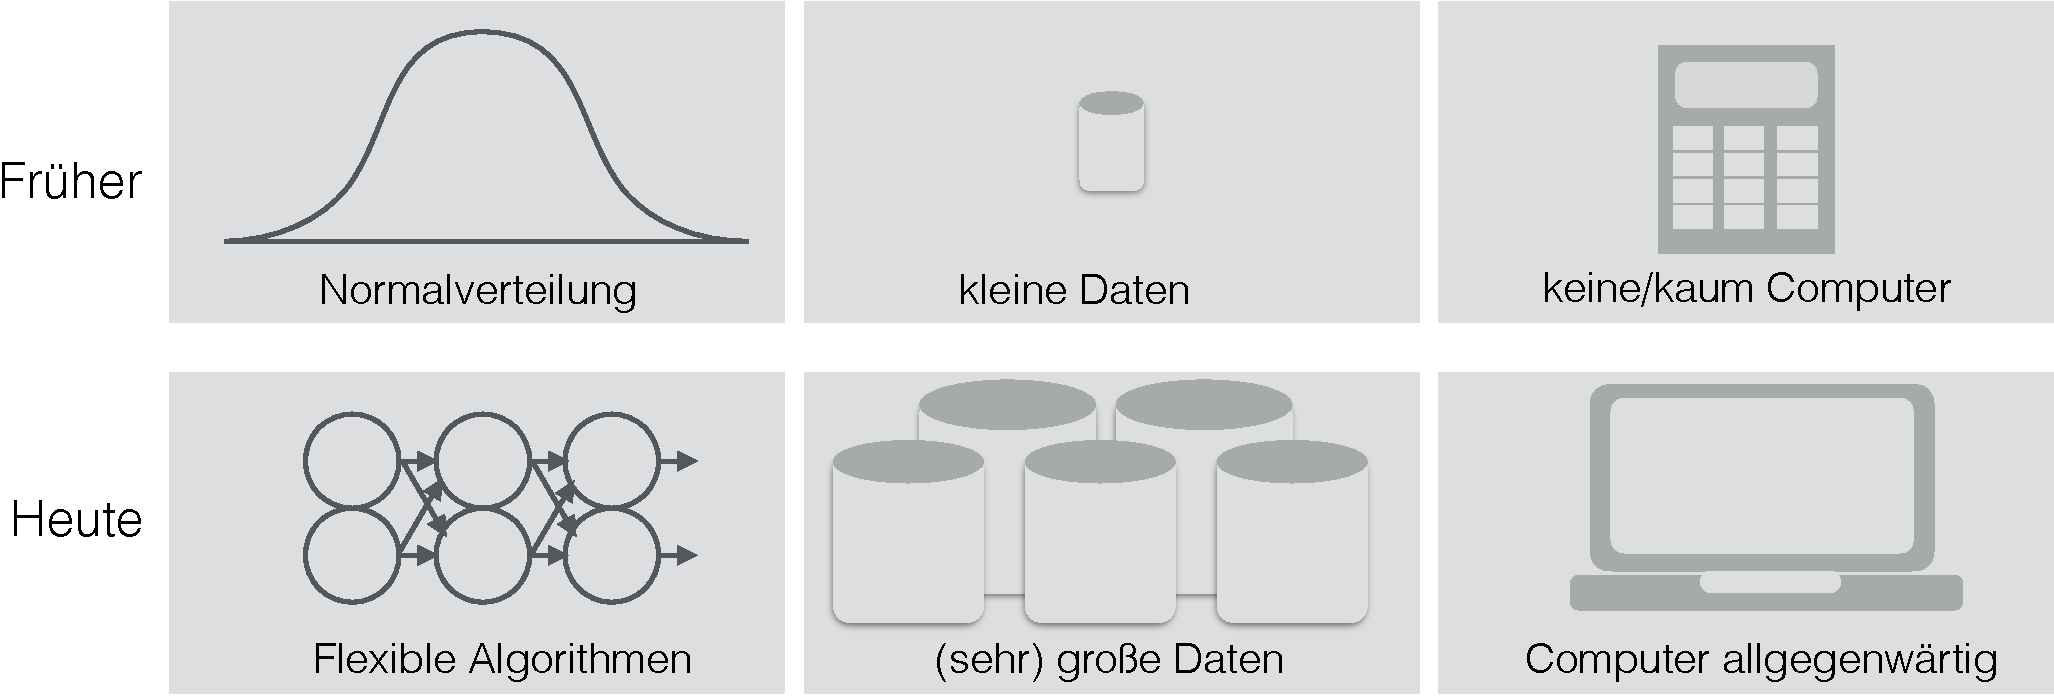
\includegraphics{images/Forschung_frueher_heute.pdf}

Zu Themen, die heute zu den dynamischten Gebieten der Datenanalyse
gehören, die aber früher keine große Rolle spielten, gehören (Hardin et
al. \protect\hyperlink{ref-hardin2015data}{2015}):

\begin{itemize}
\tightlist
\item
  Nutzung von Datenbanken und anderen Data Warehouses
\item
  Daten aus dem Internet automatisch einlesen (``scraping'')
\item
  Genanalysen mit Tausenden von Variablen
\item
  Gesichtserkennung
\end{itemize}

Es gibt bisher noch relativ wenig \emph{deutschsprachige} Bücher für
moderne Datenanalyse; es ist zu erwarten, dass sich dies bald ändert.
Dieses Buch soll beitragen, diese Lücke zu füllen. Sie werden einige
praktische Aspekte der modernen Datenanalyse lernen. Es ist ein
Grundlagenkurs; dieses Buch ist nicht für Experten geschrieben und durch
das Lesen wird man auch kein Experte. Aber man erwirbt Grundkenntnisse.
Das didaktische Konzept beruht auf einem induktiven, intuitiven
Lehr-Lern-Ansatz. Auf Formeln und mathematische Hintergründe wurde
weitestgehend verzichtet.

Im Gegensatz zu anderen Statistik-Büchern steht hier die Umsetzung mit R
deutlich stärker im Vordergrund. Dies hat pragmatische Gründe: Möchte
man Daten einer statistischen Analyse unterziehen, so muss man sie
zumeist erst aufbereiten; oft mühselig aufbereiten. Selten kann man den
Luxus genießen, einfach ``nur'', nach Herzenslust sozusagen, ein
Feuerwerk an multivariater Statistik zu entzünden. Zuvor gilt es, die
Daten aufzubereiten, umzuformen, zu prüfen und zusammenzufassen. Diesem
Teil ist hier recht ausführlich Rechnung getragen.

``Statistical thinking'' sollte, so eine verbreitete Idee, im Zentrum
oder als Ziel einer Statistik-Ausbildung stehen (Wild and Pfannkuch
\protect\hyperlink{ref-wild1999statistical}{1999}). Es ist die Hoffnung
der Autoren dieses Buches, dass das praktische Arbeiten (im Gegensatz zu
einer theoretischen Fokus) zur Entwicklung einer Kompetenz im
statistischen Denken beiträgt.‹

Außerdem spielt die Visualisierung von Daten eine große Rolle. Zum einen
könnte der Grund einfach sein, dass Diagramme ansprechen und gefallen
(einige/n Menschen). Zum anderen bieten Diagramme bei umfangreichen
Daten Einsichten, die sonst leicht wortwörtlich überersehen würden.

\emph{R-Pseudo-Syntax}: R ist (momentan) die führende Umgebung für
Datenanalyse. Entsprechend zentral ist R in diesem Kurs. Zugebenermaßen
braucht es etwas Zeit, bis man ein paar Brocken ``Errisch'' spricht. Um
den Einstieg zu erleichern, ist Errisch auf Deutsch übersetzt an einigen
Stellen, wo mir dies besonders hilfreich erschien. Diese Stellen sind
mit diesem Symbol

\includegraphics[width=0.05000\textwidth]{images/pseudocode.png}
gekennzeichnet (für R-Pseudo-Syntax).

\emph{Achtung, Falle}: Schwierige oder fehlerträchtige Stellen sind mit
diesem Symbol

\includegraphics[width=0.05000\textwidth]{images/caution.png} markiert.

\emph{Übungsaufgaben}: Das Skript beinhaltet pro Kapitel Übungsaufgaben
oder/und Testfragen. Auf diese wird so

\includegraphics[width=0.05000\textwidth]{images/exercises.png}
verwiesen.

Ansonsten: Wenn Ihnen R diesen Smiley präsentiert, dann sind Sie am Ziel
Ihrer Träume:

\includegraphics[width=0.05000\textwidth]{images/love.png}.

Dieses Skript wurde mit dem Paket \texttt{bookdown} (Xie
\protect\hyperlink{ref-xie2015}{2015}) erstellt, welches wiederum stark
auf den Paketen \texttt{knitr} (Xie
\protect\hyperlink{ref-xie2015}{2015}) und \texttt{rmarkdown} (Allaire
et al.
\protect\hyperlink{ref-rmarkdown}{2016}\protect\hyperlink{ref-rmarkdown}{a})
beruht. Diese Pakete stellen verblüffende Funktionalität zur Verfügung
als freie Software (frei wie in Bier und frei wie in Freiheit).

Aus Gründen des Lesbarkeit wird das männliche Generikum verwendet,
welches Frauen und Männer in gleichen Maßen ansprechen soll.

Die Bildnachweise sind in folgenden Muster aufgebaut: Nummer (Verweis)
des Bildes, Names des Autors, Titel, Quelle (URL), Lizenz, Abrufdatum.

\begin{itemize}
\tightlist
\item
  @ref(fig:modellieren\_plot), Sebastian Unrau, ohne Titel,
  \url{https://unsplash.com/photos/CoD2Q92UaEg}, CC0, 2017-02-12
\end{itemize}

Alle verwendeten Datensätze und R-Pakete finden sich im
Literaturverzeichnis; im Text werden Pakete nicht zitiert.

\pagenumbering{arabic}

\chapter*{I GRUNDLAGEN}\label{i-grundlagen}
\addcontentsline{toc}{chapter}{I GRUNDLAGEN}

\chapter{Rahmen}\label{rahmen}

In diesem Skript geht es um die Praxis der Datenanalyse. Mit Rahmen ist
das ``Drumherum'' oder der Kontext der eigentlichen Datenanalyse
gemeint. Dazu gehören einige praktische Vorbereitungen und ein paar
Überlegungen. Zum Beispiel brauchen wir einen Überblick über das Thema.
Voila:

\begin{center}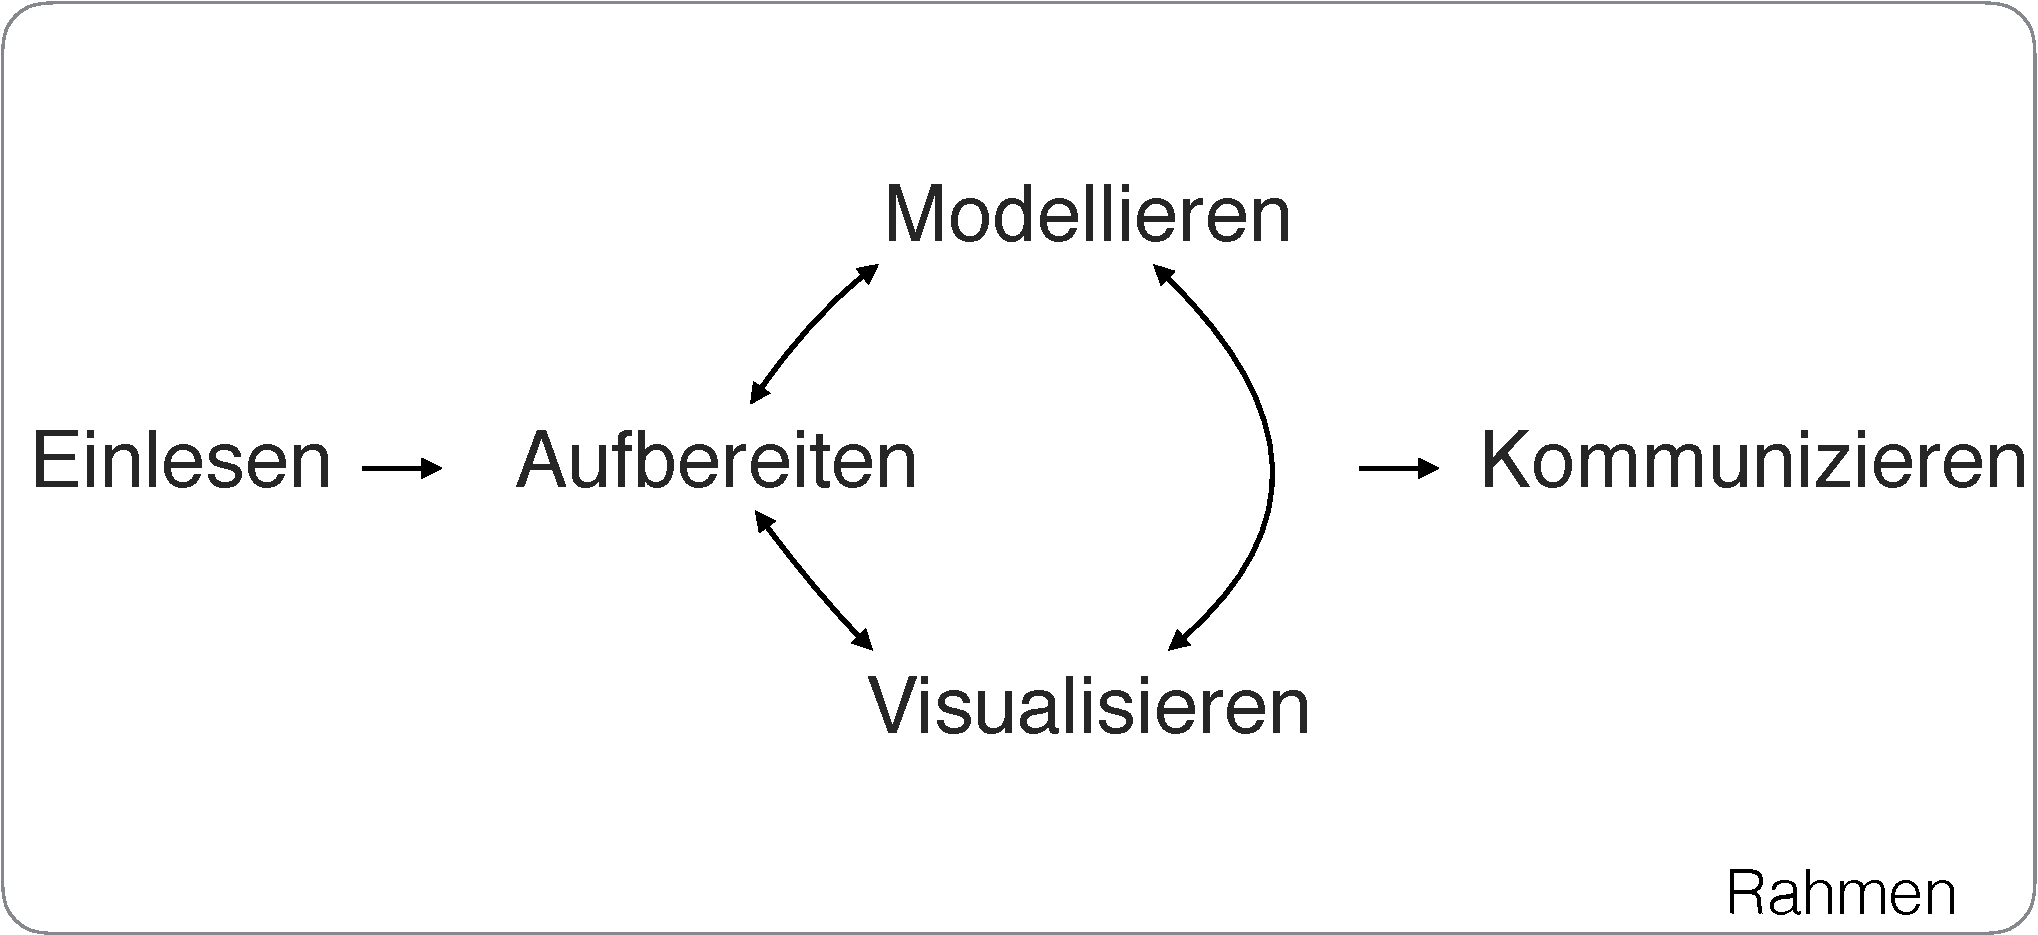
\includegraphics[width=0.7\linewidth]{images/Prozess_Datenanalyse} \end{center}

Datenanalyse, praktisch betrachtet, kann man in fünf Schritte einteilen
(Wickham and Grolemund \protect\hyperlink{ref-r4ds}{2016}). Zuerst muss
man die Daten \emph{einlesen}, die Daten also in R (oder einer anderen
Software) verfügbar machen (laden). Fügen wir hinzu: In \emph{schöner
Form} verfügbar machen; man nennt dies auch \emph{tidy data}{[}hört sich
cooler an.{]}. Sobald die Daten in geeigneter Form in R geladen sind,
folgt das \emph{Aufbereiten}. Das beinhaltet Zusammenfassen, Umformen
oder Anreichern je nach Bedarf. Ein nächster wesentlicher Schritt ist
das \emph{Visualisieren} der Daten. Ein Bild sagt bekanntlich mehr als
viele Worte. Schließlich folgt das \emph{Modellieren} oder das
Hypothesen prüfen: Man überlegt sich, wie sich die Daten erklären lassen
könnten. Zu beachten ist, dass diese drei Schritte - Aufbereiten,
Visualisieren, Modellieren - keine starre Abfolge sind, sondern eher ein
munteres Hin-und-Her-Springen, ein aufbauendes Abwechseln. Der letzte
Schritt ist das \emph{Kommunizieren} der Ergebnisse der Analyse - nicht
der Daten. Niemand ist an Zahlenwüsten interessiert; es gilt, spannende
Einblicke zu vermitteln.

Der Prozess der Datenanalyse vollzieht sich nicht im luftleeren Raum,
sondern ist in einem \emph{Rahmen} eingebettet. Dieser beinhaltet
praktische Aspekte - wie Software, Datensätze - und grundsätzliche
Überlegungen - wie Ziele und Grundannahmen.

\section{Software}\label{software}

Als Haupt-Analysewerkzeug nutzen wir R; daneben wird uns die sog.
``Entwicklungsumgebung'' RStudio einiges an komfortabler Funktionalität
bescheren. Eine Reihe von R-Paketen (``Packages''; d.h. Erweiterungen)
werden wir auch nutzen. R ist eine recht alte Sprache; viele Neuerungen
finden in Paketen Niederschlag, da der ``harte Kern'' von R lieber nicht
so stark geändert wird. Stellen Sie sich vor: Seit 29 Jahren nutzen Sie
eine Befehl, der Ihnen einen Mittelwert ausrechnet, sagen wir die
mittlere Anzahl von Tassen Kaffee am Tag. Und auf einmal wird der
Mittelwert anders berechnet?! Eine Welt stürzt ein! Naja, vielleicht
nicht ganz so tragisch in dem Beispiel, aber grundsätzlich sind
Änderungen in viel benutzen Befehlen potenziell problematisch. Das ist
wohl ein Grund, warum sich am ``R-Kern'' nicht so viel ändert. Die
Innovationen in R passieren in den Paketen. Und es gibt viele davon; als
ich diese Zeilen schreibe, sind es fast schon 10.000! Genauer: 9937 nach
dieser Quelle: \url{https://cran.r-project.org/web/packages/}.

\subsection{R und RStudio
installieren}\label{r-und-rstudio-installieren}

Setzt natürlich voraus, dass R installiert ist. Sie können R unter
\url{https://cran.r-project.org} herunterladen und installieren (für
Windows, Mac oder Linux). RStudio finden Sie auf der gleichnamigen
Homepage: \url{https://www.rstudio.com}; laden Sie die
``Desktop-Version'' für Ihr Betriebssystem herunter.

Die Oberfläche von R, die ``Console'', sieht so aus:

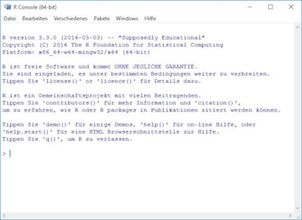
\includegraphics{images/R-small.jpg}
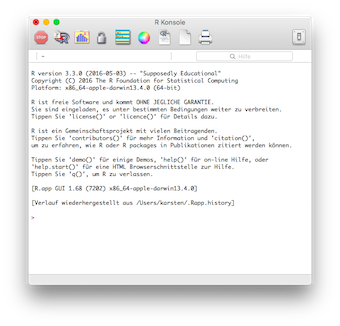
\includegraphics{images/R-Mac-small.png}

Die Oberfläche von RStudio sieht (unter allen Betriebssystemen etwa
gleich) so aus:

\begin{center}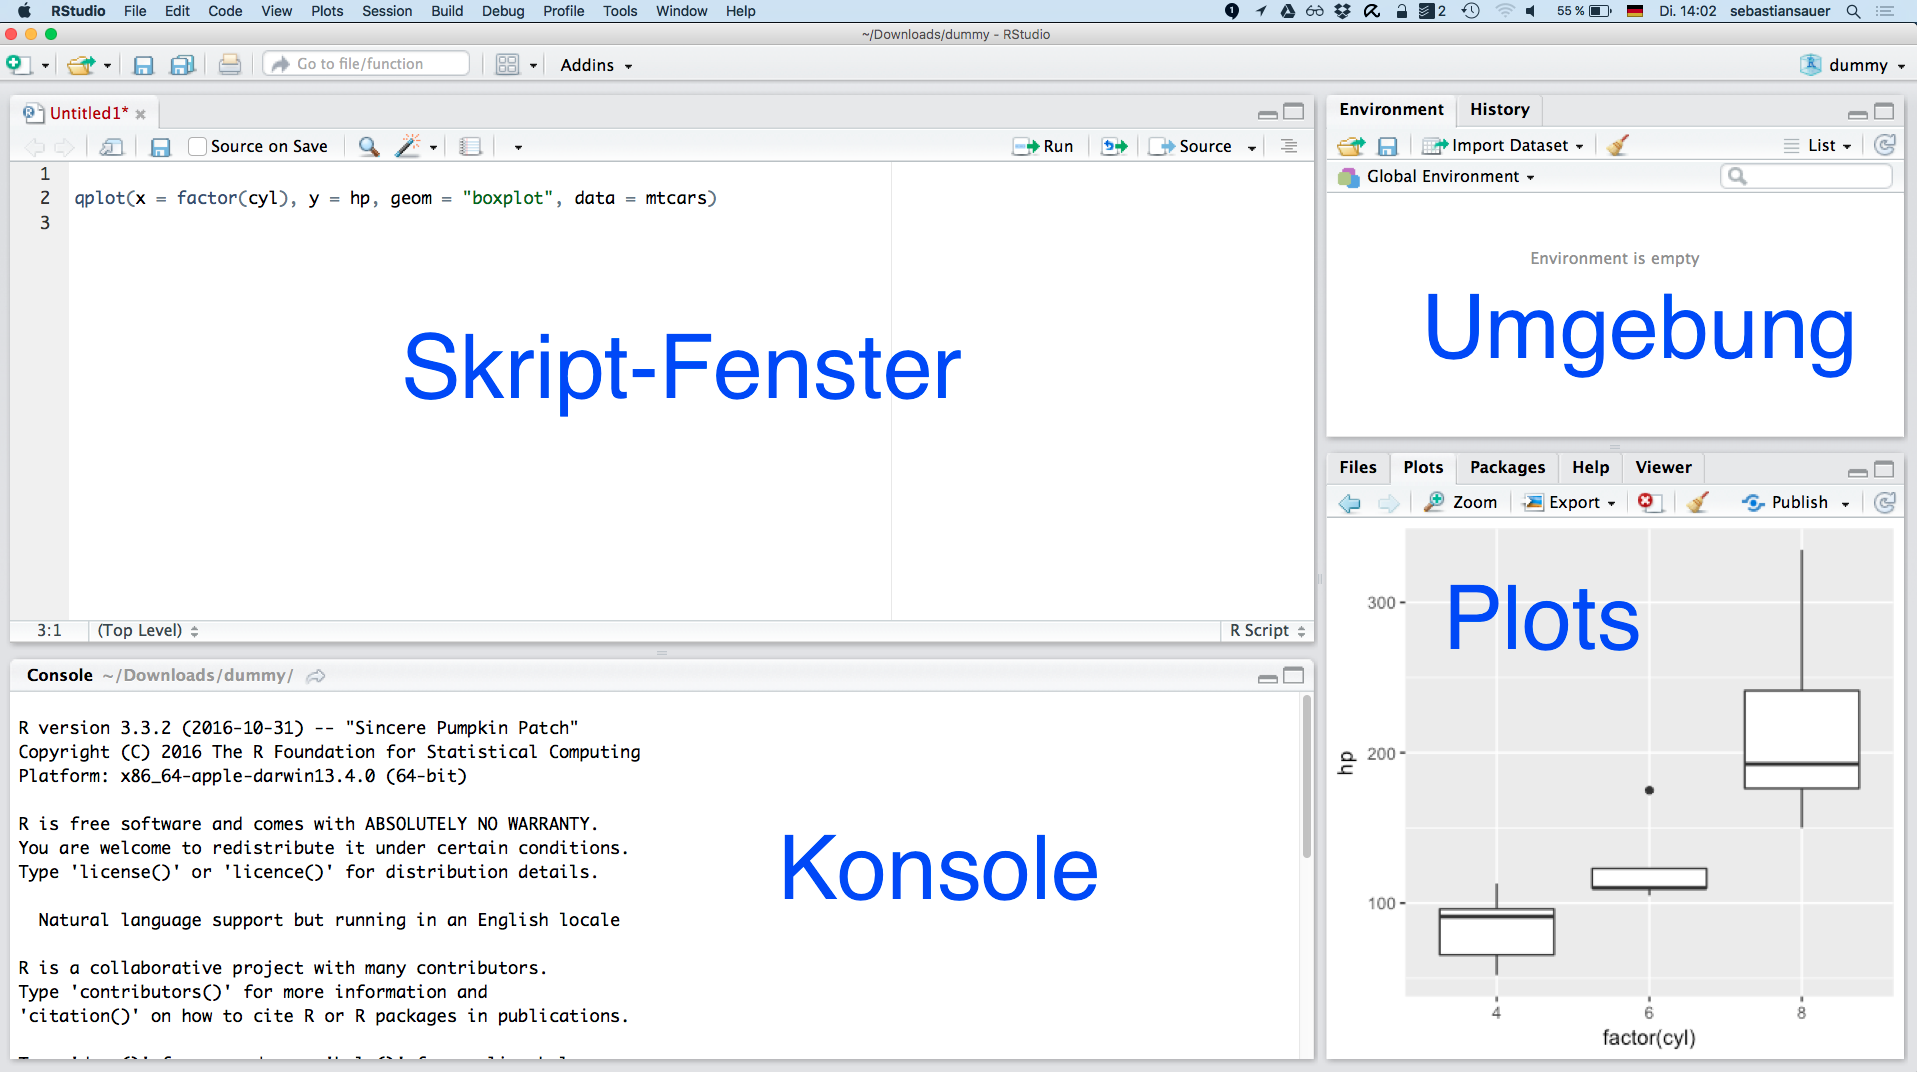
\includegraphics[width=0.7\linewidth]{images/RStudio-Screenshot} \end{center}

\subsection{Hilfe! R tut nicht so wie ich das
will}\label{hilfe-r-tut-nicht-so-wie-ich-das-will}

\begin{quote}
Manntje, Manntje, Timpe Te,\\
Buttje, Buttje inne See,\\
myne Fru de Ilsebill\\
will nich so, as ik wol will.
\end{quote}

\emph{Gebrüder Grimm, Märchen vom Fischer und seiner Frau\footnote{\url{https://de.wikipedia.org/wiki/Vom_Fischer_und_seiner_Frau}}}

Ihr R startet nicht oder nicht richtig? Die drei wichtigsten Heilmittel
sind:

\begin{enumerate}
\def\labelenumi{\arabic{enumi}.}
\tightlist
\item
  Schließen Sie die Augen für eine Minute. Denken Sie an etwas Schönes
  und was Rs Problem sein könnte.
\item
  Schalten Sie den Rechner aus und probieren Sie es morgen noch einmal.
\item
  Googeln.
\end{enumerate}

Sorry für die schnottrigen Tipps. Aber: Es passiert allzu leicht, dass
man Fehler wie diese macht:

\begin{itemize}
\tightlist
\item
  \texttt{install.packages(dplyr)}
\item
  \texttt{install.packages("dliar")}
\item
  \texttt{install.packages("derpyler")}
\item
  \texttt{install.packages("dplyr")\ \ \#\ dependencies\ vergessen}
\item
  Keine Internet-Verbindung
\item
  \texttt{library(dplyr)\ \ \#\ ohne\ vorher\ zu\ installieren}
\end{itemize}

Wenn R oder RStudio dann immer noch nicht starten oder nicht richtig
laufen, probieren Sie dieses:

\begin{itemize}
\item
  Sehen Sie eine Fehlermeldung, die von einem fehlenden Paket spricht
  (z.B. ``Package `Rcpp' not available'') oder davon spricht, dass ein
  Paket nicht installiert werden konnte (z.B. ``Package `Rcpp' could not
  be installed'' oder ``es gibt kein Paket namens `Rcpp'\,'' oder
  ``unable to move temporary installation XXX to YYY''), dann tun Sie
  folgendes:
\item
  Schließen Sie R und starten Sie es neu. - Installieren Sie das oder
  die angesprochenen Pakete mit
  \texttt{install.packages("name\_des\_pakets",\ dependencies\ =\ \ TRUE)}
  oder mit dem entsprechenden Klick in RStudio. - Starten Sie das
  entsprechende Paket mit \texttt{library(paket\_name)}.
\item
  Gerade bei Windows 10 scheinen die Schreibrechte für R (und damit
  RStudio oder RComannder) eingeschränkt zu sein. Ohne Schreibrechte
  kann R aber nicht die Pakete (``packages'') installieren, die Sie für
  bestimmte R-Funktionen benötigen. Daher schließen Sie R bzw. RStudio
  und suchen Sie das Icon von R oder wenn Sie RStudio verwenden von
  RStudio. Rechtsklicken Sie das Icon und wählen Sie ``als Administrator
  ausführen''. Damit geben Sie dem Programm Schreibrechte. Jetzt können
  Sie etwaige fehlende Pakete installieren.
\item
  Ein weiterer Grund, warum R bzw. RStudio die Schreibrechte verwehrt
  werden könnnten (und damit die Installation von Paketen), ist ein
  Virenscanner. Der Virenscanner sagt, nicht ganz zu Unrecht: ``Moment,
  einfach hier Software zu installieren, das geht nicht, zu
  gefährlich''. Grundsätzlich gut, in diesem Fall unnötig. Schließen Sie
  R/RStudio und schalten Sie dann den Virenscanner \emph{komplett} (!)
  aus. Öffnen Sie dann R/RStudio wieder und versuchen Sie fehlende
  Pakete zu installieren.
\item
  Läuft der RCommander unter Mac nicht, dann prüfen Sie, ob Sie X11
  (synonym: XQuartz) installiert haben. X11 muss installiert sein, damit
  der RCommander unter Mac läuft.
\item
  Die ``app nap'' Funktion beim Mac kann den RCommander empfindlich
  ausbremsen. Schalten Sie diese Funktion aus z.B. im RCommander über
  \texttt{Tools\ -\ Manage\ Mac\ OS\ X\ app\ nap\ for\ R.app}.
\end{itemize}

\subsection{Hier werden Sie geholfen}\label{hier-werden-sie-geholfen}

Es ist keine Schande, nicht alle Befehle der ca. 10,000 R-Pakete
auswendig zu wissen. Schlauer ist, zu wissen, wo man Antworten findet.
Hier eine Auswahl:

\begin{itemize}
\item
  Zu diesen Paketen gibt es gute ``Spickzettel'' (cheatsheets): ggplot2,
  RMarkdown, dplyr, tidyr. Klicken Sie dazu in RStudio auf \emph{Help
  \textgreater{} Cheatsheets \textgreater{} \ldots{}} oder gehen Sie auf
  \url{https://www.rstudio.com/resources/cheatsheets/}.
\item
  In RStudio gibt es eine Reihe (viele) von Tastaturkürzlen (Shortcuts),
  die Sie hier finden: \emph{Tools \textgreater{} Keyboard Shortcuts
  Help}.
\item
  Für jeden Befehl (d.i. Funktion) können Sie mit \texttt{?} Hilfe
  erhalten; probieren Sie z.B. \texttt{?mean}.
\item
  Im Internet finden sich zuhauf Tutorials.
\item
  Die bekannteste Seite, um Fragen rund um R zu diskutieren ist:
  \url{http://stackoverflow.com}.
\end{itemize}

\subsection{Die Denk- und Gefühlswelt von
R}\label{die-denk--und-gefuhlswelt-von-r}

\begin{itemize}
\item
  Wenn Sie RStudio starten, startet R automatisch auch. Starten Sie
  daher, wenn Sie RStudio gestartet haben, \emph{nicht} noch extra R.
  Damit hätten Sie sonst zwei Instanzen von R laufen, was zu
  Verwirrungen (bei R und beim Nutzer) führen kann.
\item
  Ein neues R-Skript im RStudio können Sie z.B. öffnen mit
  \texttt{File-New\ File-R\ \ Script}.
\item
  R-Skripte können Sie speichern (\texttt{File-Save}) und öffnen.
\item
  R-Skripte sind einfache Textdateien, die jeder Texteditor verarbeiten
  kann. Nur statt der Endung \texttt{txt}, sind R-Skripte stolzer Träger
  der Endung \texttt{R}. Es bleibt aber eine schnöde Textdatei.
\item
  Bei der Installation von Paketen mit
  \texttt{install.packages("name\_des\_pakets")} sollte stets der
  Parameter \texttt{dependencies\ =\ TRUE} angefügt werden. Also
  \texttt{install.packages("name\_des\_pakets",\ dependencies\ =\ TRUE)}.
  Hintergrund ist: Falls das zu installierende Paket seinerseits Pakete
  benötigt, die noch nicht installiert sind (gut möglich), dann werden
  diese sog. ``dependencies'' gleich mitinstalliert (wenn Sie
  \texttt{dependencies\ =\ TRUE} setzen).
\item
  Hier finden Sie weitere Hinweise zur Installation des RCommanders:
  \url{http://socserv.socsci.mcmaster.ca/jfox/Misc/Rcmdr/installation-notes.html}.
\item
  Sie müssen online sein, um Packages zu installieren.
\item
  Die ``app nap'' Funktion beim Mac kann den RCommander empfindlich
  ausbremsen. Schalten Sie diese Funktion aus z.B. im RCommander über
  \texttt{Tools\ -\ Manage\ Mac\ OS\ X\ app\ nap\ for\ R.app}.
\end{itemize}

Verwenden Sie möglichst die neueste Version von R, RStudio und Ihres
Betriebssystems. Ältere Versionen führen u.U. zu Problemen; je älter,
desto Problem\ldots{} Updaten Sie Ihre Packages regelmäßig z.B. mit
\texttt{update.packages()} oder dem Button ``Update'' bei RStudio
(Reiter \texttt{Packages}).

R zu lernen kann hart sein. Ich weiß, wovon ich spreche. Wahrscheinlich
eine spirituelle Prüfung in Geduld und Hartnäckigkeit\ldots{} Tolle
Gelegenheit, sich in diesen Tugenden zu trainieren :-)

\subsection{Pakete installieren}\label{pakete-installieren}

Ein R-Paket, welches für die praktische Datenanalyse praktisch ist,
heißt \texttt{dplyr}. Wir werden viel mit diesem Paket arbeiten. Bitte
installieren Sie es schon einmal, sofern noch nicht geschehen:

\begin{Shaded}
\begin{Highlighting}[]
\KeywordTok{install.packages}\NormalTok{(}\StringTok{"dplyr"}\NormalTok{, }\DataTypeTok{dependencies =} \OtherTok{TRUE}\NormalTok{) }
\end{Highlighting}
\end{Shaded}

Übrigens, das \texttt{dependencies\ =\ TRUE} sagt sinngemäß ``Wenn das
Funktionieren von dplyr noch von anderen Paketen abhängig ist (es also
Abhängigkeiten (dependencies) gibt), dann installiere die gleich mal
mit''.

\BeginKnitrBlock{rmdcaution}
Beim Installieren von R-Paketen könnten Sie gefragt werden, welchen
``Mirror'' Sie verwenden möchten. Das hat folgenden Hintergrund:
R-Pakete sind in einer Art ``App-Store'', mit Namen CRAN (Comprehense R
Archive Network) gespeichert. Damit nicht ein armer, kleiner Server
überlastet wird, wenn alle Studis dieser Welt just gerade beschließen,
ein Paket herunterzuladen, gibt es viele Kopien dieses Servers - die
``Mirrors'', Spiegelbilder. Suchen Sie sich einfach einen aus, der in
der Nähe ist.
\EndKnitrBlock{rmdcaution}

Nicht vergessen: Installieren muss man eine Software \emph{nur einmal};
\emph{starten} (laden) muss man sie jedes Mal, wenn man sie vorher
geschlossen hat und wieder nutzen möchte:

\begin{Shaded}
\begin{Highlighting}[]
\KeywordTok{library}\NormalTok{(dplyr) }
\end{Highlighting}
\end{Shaded}

Der Befehl bedeutet sinngemäß: ``Hey R, geh in die Bücherei (library)
und hole das Buch (package) dplyr!''.

\BeginKnitrBlock{rmdcaution}
Wann benutzt man bei R Anführungszeichen? Das ist etwas verwirrend im
Detail, aber die Grundegel lautet: wenn man Text anspricht. Im Beispiel
oben ``library(dplyr)'' ist ``dplyr'' hier erst mal für R nichts
Bekanntes, weil noch nicht geladen. Demnach müssten \emph{eigentlich}
Anführungsstriche stehen. Allerdings meinte ein Programmierer, dass es
doch so bequemer ist. Hat er Recht. Aber bedenken Sie, dass es sich um
die Ausnahme einer Regel handelt. Sie können also auch schreiben:
library(``dplyr'') oder library(`dplyr'); geht beides.
\EndKnitrBlock{rmdcaution}

Das Installieren und Starten anderer Pakete läuft genauso ab. Am besten
installieren Sie alle Pakete, die wir in diesem Buch benötigen auf
einmal, dann haben Sie Ruhe.

\subsection{R-Pakete für dieses Buch In diesem Buch verwenden wir die
folgenden}\label{r-pakete-fur-dieses-buch-in-diesem-buch-verwenden-wir-die-folgenden}

R-Pakete; diese müssen installiert{[}Ggf. benötigen Sie
Administrator-Rechte, um Pakete zu installieren.{]} sein und geladen:

\begin{Shaded}
\begin{Highlighting}[]
\NormalTok{Pakete }
\CommentTok{#>  [1] "tidyverse"     "readr"         "knitr"         "stringr"      }
\CommentTok{#>  [5] "car"           "nycflights13"  "ISLR"          "pdftools"     }
\CommentTok{#>  [9] "downloader"    "ggdendro"      "gridExtra"     "tm"           }
\CommentTok{#> [13] "tidytext"      "lsa"           "SnowballC"     "wordcloud"    }
\CommentTok{#> [17] "RColorBrewer"  "okcupiddata"   "reshape2"      "wesanderson"  }
\CommentTok{#> [21] "GGally"        "titanic"       "compute.es"    "corrr"        }
\CommentTok{#> [25] "rpart"         "rpart.plot"    "MASS"          "titanic"      }
\CommentTok{#> [29] "arules"        "arulesViz"     "SDMTools"      "corrplot"     }
\CommentTok{#> [33] "gplots"        "corrplot"      "scatterplot3d" "BaylorEdPsych"}
\CommentTok{#> [37] "nFactors"      "rmarkdown"     "methods"}
\end{Highlighting}
\end{Shaded}

Anstelle alle einzeln zu laden (\texttt{library} verdaut nur ein Paket
auf einmal), können wir mit etwas R-Judo alle auf einen Haps laden:

\begin{Shaded}
\begin{Highlighting}[]
\KeywordTok{lapply}\NormalTok{(Pakete, require, }\DataTypeTok{character.only =} \OtherTok{TRUE}\NormalTok{) }
\end{Highlighting}
\end{Shaded}

Der Befehl heißt auf Deutsch: ``Wende auf jedes Element von
\texttt{Pakete} den Befehl \texttt{library} an''\footnote{\url{http://stackoverflow.com/questions/8175912/load-multiple-packages-at-once}}.

Hin und wieder ist es sinnvoll, die Pakete auf den neuesten Stand zu
bringen; das geht mit \texttt{update.packages()}.

\subsection{Datensätze}\label{datensatze}

\begin{itemize}
\tightlist
\item
  Datensatz \texttt{profiles} aus dem R-Paket \{okcupiddata\} (Kim and
  Escobedo-Land \protect\hyperlink{ref-kim2015okcupid}{2015}); es
  handelt sich um Daten von einer Online-Singlebörse
\item
  Datensatz \texttt{Wage} aus dem R-Paket \{ISLR\} (James, Witten,
  Hastie, and Tibshirani
  \protect\hyperlink{ref-introstatlearning}{2013}\protect\hyperlink{ref-introstatlearning}{b});
  es handelt sich um Gehaltsdaten von US-amerikanischen Männern
\item
  Datensatz \texttt{inf\_test\_short}, hier herunterzuladen:
  \textless{}osf.io/sjhu\textgreater{} (Sauer
  \protect\hyperlink{ref-Sauer_2017}{2017}\protect\hyperlink{ref-Sauer_2017}{a});
  es handelt sich um Ergebnisse einer Statistikklausur
\item
  Datensatz \texttt{flights} aus dem R-Paket \{nycflights13\} (RITA
  \protect\hyperlink{ref-nycflights13}{2013}); es handelt sich um
  Abflüge von den New Yorker Flughäfen
\item
  Datensatz 'wo\_men`, hier herunterzuladen:
  \textless{}osf.io/ja9dw\textgreater{} (Sauer
  \protect\hyperlink{ref-Sauer_2017a}{2017}\protect\hyperlink{ref-Sauer_2017a}{b});
  es handelt sich um Körper- und Schuhgröße von Studierenden
\item
  Datensatz \texttt{tips} aus dem R-Paket \{reshape2\} (Bryant and Smith
  \protect\hyperlink{ref-bryant1995practical}{1995}); es handelt sich um
  Trinkgelder in einem Restaurant
\item
  Datensatz \texttt{extra}, hier herunterzuladen:
  \textless{}osf.io/4kgzh\textgreater{} (Sauer
  \protect\hyperlink{ref-Sauer_2016}{2016}); es handelt sich die
  Ergebnisse einer Umfrage zu Extraversion
\end{itemize}

Wir verwenden zwei Methoden, um Datensätze in R zu laden.

\begin{itemize}
\tightlist
\item
  Zum einen laden wir Datensätze aus R-Paketen, z.B. aus dem Paket
  \texttt{okcupiddata}. Dazu muss das entsprechende Paket installiert
  und geladen sein. Mit dem Befehl
  \texttt{data(name\_des\_datensatzes,\ package\ =\ "name\_des\_paketes")},
  kann man dann die Daten laden. Das Laden eines Pakets lädt noch
  \emph{nicht} die Daten des Paektes; dafür ist der Befehl \texttt{data}
  zuständig.
\end{itemize}

\begin{Shaded}
\begin{Highlighting}[]
\KeywordTok{library}\NormalTok{(okcupiddata) }\KeywordTok{data}\NormalTok{(profiles, }\DataTypeTok{package =} \StringTok{"okcupiddata"}\NormalTok{)}
\end{Highlighting}
\end{Shaded}

\begin{itemize}
\tightlist
\item
  Alternativ kann man die Daten als CSV- oder als XLS(X)-Datei
  importieren. Die Datei darf dabei sowohl auf einer Webseite als auch
  lokal (Festplatte, Stic\ldots{}) liegen.
\end{itemize}

\begin{Shaded}
\begin{Highlighting}[]
\NormalTok{Daten <-}\StringTok{ }
\KeywordTok{read.csv}\NormalTok{(}\StringTok{"https://sebastiansauer.github.io/data/tips.csv"}\NormalTok{) }
\end{Highlighting}
\end{Shaded}

Wir werden mit beiden Methoden arbeiten und ``on the job'' Details
besprechen.

\section{ERRRstkontakt}\label{errrstkontakt}

Unser erster Kontakt mit R! Ein paar Anmerkungen vorweg:

\begin{itemize}
\tightlist
\item
  R unterscheidet zwischen Groß- und Kleinbuchstaben, d.h. \texttt{Oma}
  und \texttt{oma} sind zwei verschiedene Dinge für R!
\item
  R verwendet den Punkt \texttt{.} als Dezimaltrennzeichen.
\item
  Fehlende Werte werden in R durch \texttt{NA} kodiert.
\item
  Kommentare werden mit dem Rautezeichen \texttt{\#} eingeleitet; der
  Rest der Zeile von von R dann ignoriert.
\item
  R wendet Befehle direkt an.
\item
  R ist objektorientiert, d. h. dieselbe Funktion hat evtl. je nach
  Funktionsargument unterschiedliche Rückgabewerte.
\item
  Hilfe zu einem Befehl erhält man über ein vorgestelltes Fragezeichen
  \texttt{?}.
\item
  Zusätzliche Funktionalität kann über Zusatzpakete hinzugeladen werden.
  Diese müssen ggf. zunächst installiert werden.
\item
  Mit der Pfeiltaste ``nach oben'' können Sie in der Konsole einen
  vorherigen Befehl wieder aufrufen.
\item
  Sofern Sie das Skriptfenster verwenden: einzelne Befehle aus dem
  Skriptfenster in R Studio können Sie auch mit \texttt{Str} und
  \texttt{Enter} an die Console schicken.
\end{itemize}

\subsection{R als Taschenrechner Auch wenn Statistik nicht Mathe ist, so
kann man mit
R}\label{r-als-taschenrechner-auch-wenn-statistik-nicht-mathe-ist-so-kann-man-mit-r}

auch rechnen. Geben Sie zum Üben die Befehle in der R Konsole hinter der
Eingabeaufforderung \texttt{\textgreater{}} ein und beenden Sie die
Eingabe mit \texttt{Return} bzw. \texttt{Enter}.

\begin{Shaded}
\begin{Highlighting}[]
\DecValTok{4+2} 
\CommentTok{#> [1] 6}
\end{Highlighting}
\end{Shaded}

Das Ergebnis wird direkt angezeigt. Bei

\begin{Shaded}
\begin{Highlighting}[]
\NormalTok{x <-}\StringTok{ }\DecValTok{4+2} 
\end{Highlighting}
\end{Shaded}

erscheint zunächst kein Ergebnis. Über \texttt{\textless{}-} wird der
Variable \texttt{x} der Wert \texttt{4+2} zugewiesen. Wenn Sie jetzt

\begin{Shaded}
\begin{Highlighting}[]
\NormalTok{x }
\end{Highlighting}
\end{Shaded}

eingeben, wird das Ergebnis

\begin{verbatim}
#> [1] 6
\end{verbatim}

angezeigt. Sie können jetzt auch mit \texttt{x} weiterrechnen, z.B.:

\begin{Shaded}
\begin{Highlighting}[]
\NormalTok{x/}\DecValTok{4} 
\CommentTok{#> [1] 1.5}
\end{Highlighting}
\end{Shaded}

Vielleicht fragen Sie sich was die \texttt{{[}1{]}} vor dem Ergebnis
bedeutet. R arbeitet vektororientiert, und die \texttt{{[}1{]}} zeigt
an, dass es sich um das erste (und hier auch letzte) Element des Vektors
handelt.

\section{Was ist Statistik? Wozu ist sie
gut?}\label{was-ist-statistik-wozu-ist-sie-gut}

Zwei Fragen bieten sich sich am Anfang der Beschäftigung mit jedem Thema
an: Was ist die Essenz des Themas? Warum ist das Thema (oder die
Beschäftigung damit) wichtig?

Was ist Stististik? \emph{Eine} Antwort dazu ist, dass Statistik die
Wissenschaft von Sammlung, Analyse, Interpretation und Kommunikation von
Daten ist mithilfe mathematischer Verfahren ist und zur
Entscheidungshilfe beitragen solle (\emph{The Oxford Dictionary of
Statistical Terms} \protect\hyperlink{ref-oxford}{2006}; Romeijn
\protect\hyperlink{ref-sep-statistics}{2016}). Damit hätten wir auch den
Unterschied zur schnöden Datenanalyse (ein Teil der Statistik)
herausgemeiselt. Statistik wird häufig in die zwei Gebiete
\emph{deskriptive} und \emph{inferierende} Statistik eingeteilt. Erstere
fasst viele Zahlen zusammen, so dass wir den Wald statt vieler Bäume
sehen. Letztere verallgemeinert von den vorliegenden (sog.
``Stichproben-'')Daten auf eine zugrunde liegende Grundmenge
(Population). Dabei spielt die Wahrscheinlichkeitsrechnung (Stochastik)
eine große Rolle.

Aufgabe der deskriptiven Statistik ist es primär, Daten prägnant
zusammenzufassen. Aufgabe der Inferenzstatistik ist es, zu prüfen, ob
Daten einer Stichprobe auf eine Grundgesamtheit verallgemeinert werden
können.

Dabei lässt sich der Begriff ``Statistik'' als Überbegriff von
``Datenanalyse'' verstehen, wenn diese Sicht auch nicht von allen
geteilt wird (Grolemund and Wickham
\protect\hyperlink{ref-grolemund2014cognitive}{2014}). In diesem Buch
steht die Aufbereitung, Analyse, Interpretation und Kommunikation von
Daten im Vordergrund. Liegt der Schwerpunkt dieser Aktivitäten bei
computerintensiven Methoden, so wird auch von \emph{Data Science}
gesprochen, wobei der Begriff nicht einheitlich verwendet wird (Wickham
and Grolemund \protect\hyperlink{ref-r4ds}{2016}; Hardin et al.
\protect\hyperlink{ref-hardin2015data}{2015})

\emph{Daten} kann man definieren als \emph{Informationen, die in einem
Kontext stehen} (Moore
\protect\hyperlink{ref-moore1990uncertainty}{1990}), wobei eine
numerische Konnotation mitschwingt.

\emph{Modellieren} kann man als \emph{zentrale Aufgabe von Statistik}
begreifen (Cobb \protect\hyperlink{ref-cobb2007introductory}{2007};
Grolemund and Wickham
\protect\hyperlink{ref-grolemund2014cognitive}{2014}). Einfach
gesprochen, bedeutet Modellieren in diesem Sinne, ein mathematisches
Narrativ (``Geschichte'') zu finden, welches als Erklärung für gewisse
Muster in den Daten fungiert; vgl. Kap. @ref\{mod1\}.

Statistisches Modellieren läuft gewöhnlich nach folgendem Muster ab
(Grolemund and Wickham
\protect\hyperlink{ref-grolemund2014cognitive}{2014}):

\begin{verbatim}
Prämisse 1: Wenn Modell M wahr ist, dann sollten die Daten das Muster D aufweisen.
Prämisse 2: Die Daten weisen das Muster D auf.

---

Konklusion: Daher muss das Modell M wahr sein.
\end{verbatim}

Die Konklusion ist \emph{nicht} zwangsläufig richtig. Es ist falsch zu
sagen, dass dieses Argumentationsmuster - Abduktion (Peirce
\protect\hyperlink{ref-peirce1955abduction}{1955}) genannt - wahre,
sichere Schlüsse (Konklusionen) liefert. Die Konklusion \emph{kann, muss
aber nicht}, zutreffen.

Ein Beispiel: Auf dem Nachhauseweg eines langen Arbeitstags wartet, in
einer dunklen Ecke, ein Mann, der sich als Statistik-Professor vorstellt
und Sie zu einem Glücksspiel einlädt. Sofort sagen Sie zu. Der
Statistiker will 10 Mal eine Münze werfen, er setzt auf Zahl (versteht
sich). Wenn er gewinnt, bekommt er 10\euro{} von Ihnen; gewinnen Sie,
bekommen Sie 11\euro{} von ihm. Hört sich gut an, oder? Nun wirft er die
Münze zehn Mal. Was passiert? Er gewinnt 10 Mal, natürlich (so will es
die Geschichte). Sollten wir glauben, dass er ein Betrüger ist?

Ein Modell, welches wir hier verwenden könnten, lautet: Wenn die Münze
gezinkt ist (Modell M zutrifft), dann wäre diese Datnlage D (10 von 10
Treffern) wahrscheinlich - Prämisse 1. Datenlage D ist tatsächlich der
Fall; der Statistiker hat 10 von 10 Treffer erzielt - Prämisse 2. Die
Daten D ``passen'' also zum Modell M; man entscheidet sich, dass der
Professor ein Falschspieler ist.

Wichtig zu erkennen ist, dass Abduktion mit dem Wörtchen \emph{wenn}
beginnt. Also davon \emph{ausgeht}, dass ein Modell M der Fall ist (der
Professor also tatsächlich ein Betrüger ist). Dass, worüber wir
entscheiden wollen, wird also bereits vorausgesetzt. Gilt also M, wie
gut passen dann die Daten dazu?

\begin{quote}
Wie gut passen die Daten D zum Modell M?
\end{quote}

Das ist die Frage, die hier tatsächlich gestellt bzw. beantwortet wird.

Natürlich ist es keineswegs sicher, \emph{dass} das Modell gilt. Darüber
macht die Abduktion auch keine Aussage. Es könnte also sein, dass ein
anderes Modell zutrifft: Der Professor könnte ein Heiliger sein, der uns
auf etwas merkwürdige Art versucht, Geld zuzuschanzen\ldots{} Oder er
hat einfach Glück gehabt.

\begin{quote}
Statistische Modelle beantworten i.d.R. nicht, wie wahrsheinlich es ist,
dass ein Modell gilt. Statistische Modelle beurteilen, wie gut Daten zu
einem Modell passen.
\end{quote}

Häufig trifft ein Modell eine Reihe von Annahmen, die nicht immer
explizit gemacht werden, aber die klar sein sollten. Z.B. sind die
Münzwürfe unabhängig voneinander? Oder kann es sein, dass sich die Münze
``einschießt'' auf eine Seite? Dann wären die Münzwürfe nicht unabhängig
voneinander. In diesem Fall klingt das reichlich unplausibel; in anderen
Fällen kann dies eher der Fall sein\footnote{Sind z.B. die
  Prüfungsergebnisse von Schülern unabhängig voneinander? Möglicherweise
  haben sie von einem ``Superschüler'' abgeschrieben. Wenn der
  Superschüler viel weiß, dann zeigen die Abschreiber auch gute
  Leistung.}. Auch wenn die Münzwürfe unabhängig voneinander sind, ist
die Wahrscheinlichkeit für Zahl jedes Mal gleich? Hier ist es wiederum
unwahrscheinlich, dass sich die Münze verändert, ihre Masse verlagert,
so dass eine Seite Unwucht bekommt. In anderen Situationen können sich
Untersuchungsobjekte verändern (Menschen lernen manchmal etwas, sagt
man), so dass die Wahrscheinlichkeiten für ein Ereignis unterschiedlich
sein können, man dies aber nicht berücksichtigt.

\section{Verweise}\label{verweise}

\begin{itemize}
\item
  Chester Ismay erläutert einige Grundlagen von R und RStudio, die für
  Datenanalyse hilfreich sind:
  \url{https://bookdown.org/chesterismay/rbasics/}.
\item
  Roger Peng und Kollegen bieten hier einen Einstieg in Data Science mit
  R: \url{https://bookdown.org/rdpeng/artofdatascience/}
\item
  Wickam und Grolemund (\protect\hyperlink{ref-r4ds}{2016}) geben einen
  hervorragenden Überblick in das Thema dieses Buches; ihr Buch ist sehr
  zu empfehlen.
\item
  Wer einen stärker an der Statistik orientierten Zugang sucht, aber
  ``mathematisch sanft'' behandelt werden möchte, wird bei James et al.
  (\protect\hyperlink{ref-introstatlearning}{2013}\protect\hyperlink{ref-introstatlearning}{b})
  glücklich oder zumindest fündig werden.
\end{itemize}

\section{Versionshinweise}\label{versionshinweise}

\begin{Shaded}
\begin{Highlighting}[]
\KeywordTok{sessionInfo}\NormalTok{() }
\CommentTok{#> R version 3.3.2 (2016-10-31)}
\CommentTok{#> Platform: x86_64-apple-darwin13.4.0 (64-bit)}
\CommentTok{#> Running under: macOS Sierra 10.12.3}
\CommentTok{#> }
\CommentTok{#> locale:}
\CommentTok{#> [1] en_US.UTF-8/en_US.UTF-8/en_US.UTF-8/C/en_US.UTF-8/en_US.UTF-8}
\CommentTok{#> }
\CommentTok{#> attached base packages:}
\CommentTok{#> [1] grid      methods   stats     graphics  grDevices utils     datasets }
\CommentTok{#> [8] base     }
\CommentTok{#> }
\CommentTok{#> other attached packages:}
\CommentTok{#>  [1] rmarkdown_1.3        nFactors_2.3.3       lattice_0.20-34     }
\CommentTok{#>  [4] boot_1.3-18          psych_1.6.12         BaylorEdPsych_0.5   }
\CommentTok{#>  [7] scatterplot3d_0.3-38 gplots_3.0.1         corrplot_0.77       }
\CommentTok{#> [10] SDMTools_1.1-221     arulesViz_1.2-0      arules_1.5-0        }
\CommentTok{#> [13] Matrix_1.2-8         MASS_7.3-45          rpart.plot_2.1.1    }
\CommentTok{#> [16] rpart_4.1-10         corrr_0.2.1          compute.es_0.2-4    }
\CommentTok{#> [19] titanic_0.1.0        GGally_1.3.0         wesanderson_0.3.2   }
\CommentTok{#> [22] reshape2_1.4.2       okcupiddata_0.1.0    wordcloud_2.5       }
\CommentTok{#> [25] RColorBrewer_1.1-2   lsa_0.73.1           SnowballC_0.5.1     }
\CommentTok{#> [28] tidytext_0.1.2       tm_0.6-2             NLP_0.1-10          }
\CommentTok{#> [31] gridExtra_2.2.1      ggdendro_0.1-20      downloader_0.4      }
\CommentTok{#> [34] pdftools_1.0         ISLR_1.0             nycflights13_0.2.2  }
\CommentTok{#> [37] car_2.1-4            stringr_1.2.0        knitr_1.15.1        }
\CommentTok{#> [40] dplyr_0.5.0          purrr_0.2.2.9000     readr_1.0.0         }
\CommentTok{#> [43] tidyr_0.6.1          tibble_1.2           ggplot2_2.2.1       }
\CommentTok{#> [46] tidyverse_1.1.1     }
\CommentTok{#> }
\CommentTok{#> loaded via a namespace (and not attached):}
\CommentTok{#>  [1] readxl_0.1.1        backports_1.0.5     plyr_1.8.4         }
\CommentTok{#>  [4] lazyeval_0.2.0.9000 splines_3.3.2       digest_0.6.12      }
\CommentTok{#>  [7] foreach_1.4.3       htmltools_0.3.5     viridis_0.3.4      }
\CommentTok{#> [10] gdata_2.17.0        magrittr_1.5        cluster_2.0.5      }
\CommentTok{#> [13] gclus_1.3.1         modelr_0.1.0        R.utils_2.5.0      }
\CommentTok{#> [16] colorspace_1.3-2    rvest_0.3.2         haven_1.0.0        }
\CommentTok{#> [19] jsonlite_1.3        lme4_1.1-12         zoo_1.7-14         }
\CommentTok{#> [22] iterators_1.0.8     registry_0.3        gtable_0.2.0       }
\CommentTok{#> [25] MatrixModels_0.4-1  kernlab_0.9-25      prabclus_2.2-6     }
\CommentTok{#> [28] DEoptimR_1.0-8      SparseM_1.74        scales_0.4.1       }
\CommentTok{#> [31] mvtnorm_1.0-5       DBI_0.5-1           Rcpp_0.12.9        }
\CommentTok{#> [34] viridisLite_0.1.3   foreign_0.8-67      mclust_5.2.2       }
\CommentTok{#> [37] stats4_3.3.2        DT_0.2              vcd_1.4-3          }
\CommentTok{#> [40] htmlwidgets_0.8     httr_1.2.1          fpc_2.1-10         }
\CommentTok{#> [43] modeltools_0.2-21   reshape_0.8.6       R.methodsS3_1.7.1  }
\CommentTok{#> [46] flexmix_2.3-13      nnet_7.3-12         munsell_0.4.3      }
\CommentTok{#> [49] tools_3.3.2         broom_0.4.2         evaluate_0.10      }
\CommentTok{#> [52] yaml_2.1.14         robustbase_0.92-7   caTools_1.17.1     }
\CommentTok{#> [55] dendextend_1.4.0    nlme_3.1-130        whisker_0.3-2      }
\CommentTok{#> [58] quantreg_5.29       slam_0.1-40         R.oo_1.21.0        }
\CommentTok{#> [61] xml2_1.1.1          tokenizers_0.1.4    pbkrtest_0.4-6     }
\CommentTok{#> [64] plotly_4.5.6        stringi_1.1.2       forcats_0.2.0      }
\CommentTok{#> [67] trimcluster_0.1-2   nloptr_1.0.4        lmtest_0.9-35      }
\CommentTok{#> [70] bitops_1.0-6        seriation_1.2-1     R6_2.2.0           }
\CommentTok{#> [73] bookdown_0.3        TSP_1.1-5           KernSmooth_2.23-15 }
\CommentTok{#> [76] janeaustenr_0.1.4   codetools_0.2-15    gtools_3.5.0       }
\CommentTok{#> [79] assertthat_0.1      rprojroot_1.2       mnormt_1.5-5       }
\CommentTok{#> [82] diptest_0.75-7      mgcv_1.8-16         parallel_3.3.2     }
\CommentTok{#> [85] hms_0.3             class_7.3-14        minqa_1.2.4        }
\CommentTok{#> [88] lubridate_1.6.0     base64enc_0.1-3}
\end{Highlighting}
\end{Shaded}

\chapter{Tidy Data - Daten sauber
einlesen}\label{tidy-data---daten-sauber-einlesen}

\begin{figure}

{\centering 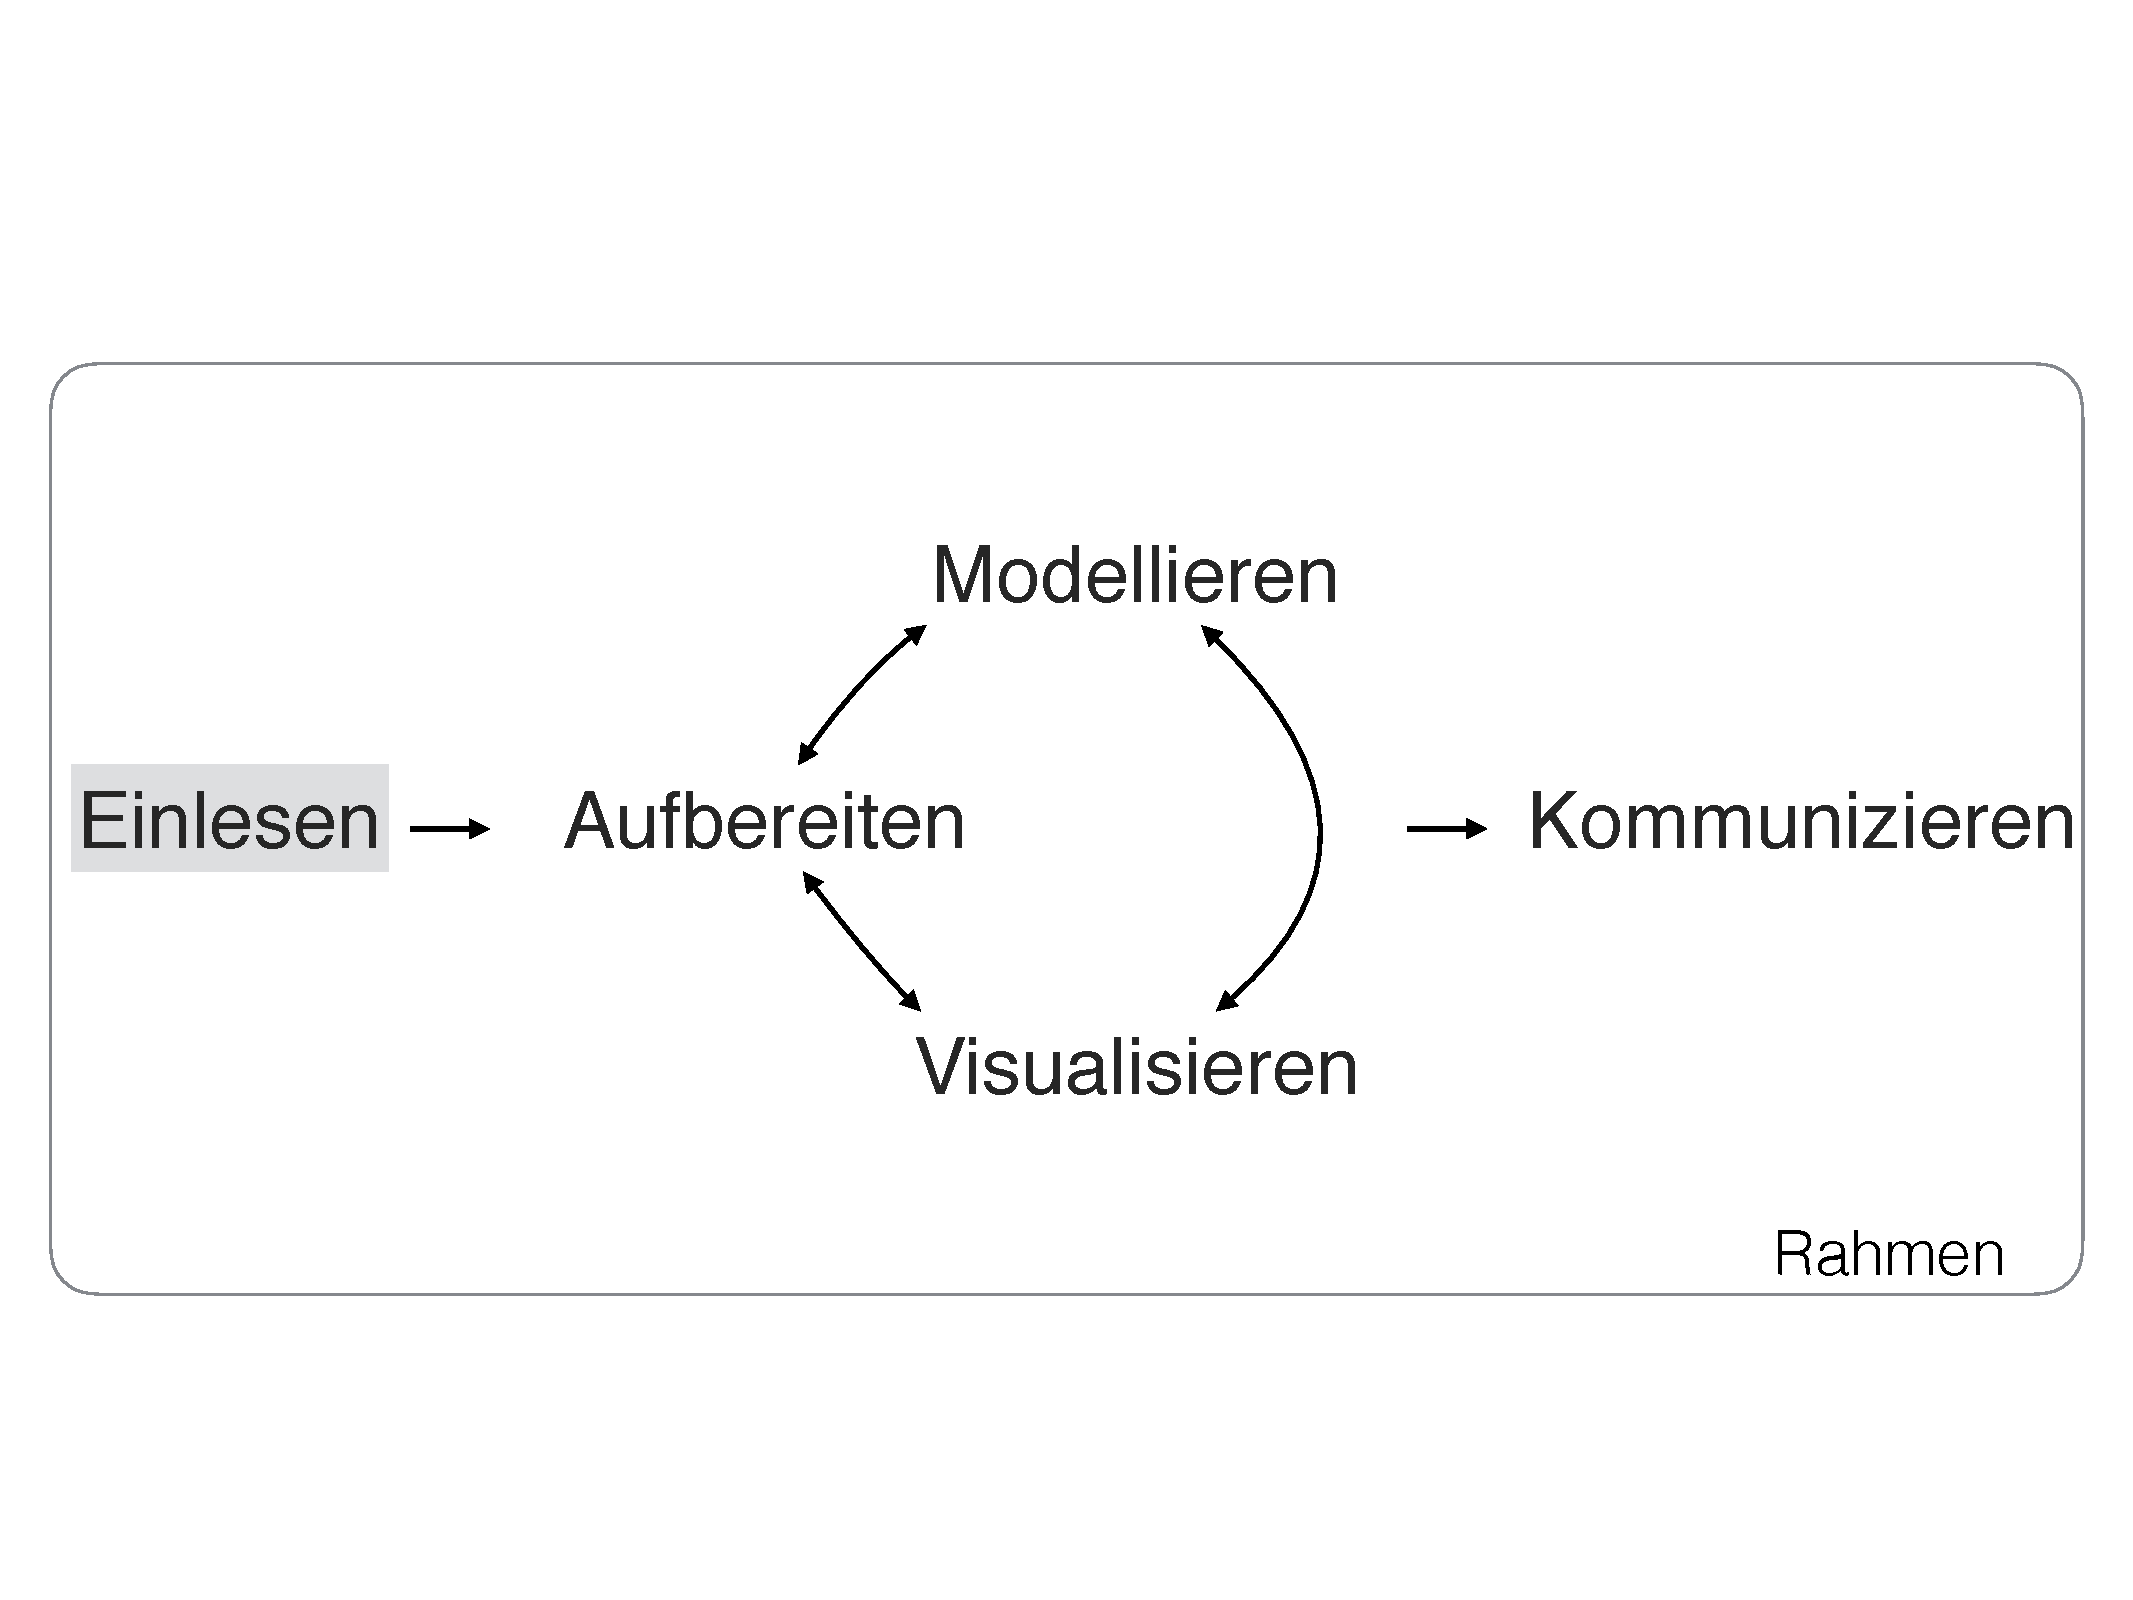
\includegraphics[width=0.7\linewidth]{images/Einlesen} 

}

\caption{Daten sauber einlesen}\label{fig:step-Einlesen}
\end{figure}

\section{Daten in R importieren}\label{daten-in-r-importieren}

In R kann man ohne Weiteres verschiedene, gebräuchliche (Excel) oder
weniger gebräuchliche (Feather\footnote{\url{https://cran.r-project.org/web/packages/feather/index.html}})
Datenformate einlesen. In RStudio lässt sich dies z.B. durch einen
schnellen Klick auf \texttt{Import\ Dataset} im Reiter
\texttt{Environment} erledigen. Dabei wird im Hintergrund das Paket
\texttt{readr} verwendet (Wickham, Hester, and Francois
\protect\hyperlink{ref-readr}{2016}\protect\hyperlink{ref-readr}{a})
(die entsprechende Syntax wird in der Konsole ausgegeben, so dass man
sie sich anschauen und weiterverwenden kann).

Am einfachsten ist es, eine Excel-Datei über die RStudio-Oberfläche zu
importieren; das ist mit ein paar Klicks geschehen:

\begin{figure}

{\centering 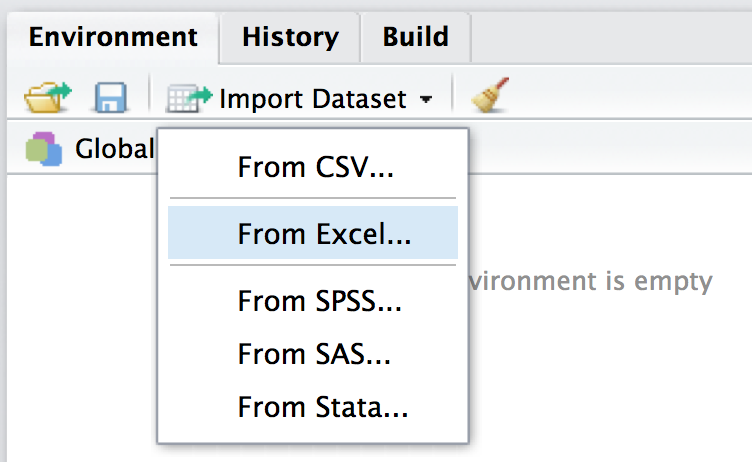
\includegraphics[width=0.5\linewidth]{images/import_RStudio} 

}

\caption{Daten einlesen (importieren) mit RStudio}\label{fig:data-import-RStudio}
\end{figure}

Es ist für bestimmte Zwecke sinnvoll, nicht zu klicken, sondern die
Syntax einzutippen. Zum Beispiel: Wenn Sie die komplette Analyse als
Syntax in einer Datei haben (eine sog. ``Skriptdatei''), dann brauchen
Sie (in RStudio) nur alles auszuwählen und auf \texttt{Run} zu klicken,
und die komplette Analyse läuft durch! Die Erfahrung zeigt, dass das ein
praktisches Vorgehen ist.

Die gebräuchlichste Form von Daten für statistische Analysen ist
wahrscheinlich das CSV-Format. Das ist ein einfahes Format, basierend
auf einer Textdatei. Schauen Sie sich mal diesen Auszug aus einer
CSV-Datei an.

\begin{verbatim}
"ID","time","sex","height","shoe_size"
"1","04.10.2016 17:58:51",NA,160.1,40
"2","04.10.2016 17:58:59","woman",171.2,39
"3","04.10.2016 18:00:15","woman",174.2,39
"4","04.10.2016 18:01:17","woman",176.4,40
"5","04.10.2016 18:01:22","man",195.2,46
\end{verbatim}

Erkenenn Sie das Muster? Die erste Zeile gibt die ``Spaltenköpfe''
wieder, also die Namen der Variablen. Hier sind es 5 Spalten; die vierte
heißt ``shoe\_size''. Die Spalten sind offenbar durch Komma \texttt{,}
voneinander getrennt. Dezimalstellen sind in amerikanischer Manier mit
einem Punkt \texttt{.} dargestellt. Die Daten sind ``rechteckig''; alle
Spalten haben gleich viele Zeilen und umgekehrt alle Spalten gleich
viele Zeilen. Man kann sich diese Tabelle gut als Excel-Tabelle mit
Zellen vorstellen, in denen z.B. ``ID'' (Zelle oben links) oder ``46''
(Zelle unten rechts) steht.

An einer Stelle steht \texttt{NA}. Das ist Errisch für ``fehlender
Wert''. Häufig wird die Zelle auch leer gelassen, um auszudrücken, dass
ein Wert hier fehlt (hört sich nicht ganz doof an). Aber man findet alle
möglichen Ideen, um fehlende Werte darzustellen. Ich rate von allen
anderen ab; führt nur zu Verwirrung.

Lesen wir diese Daten jetzt ein:

\begin{Shaded}
\begin{Highlighting}[]
\NormalTok{if (!}\KeywordTok{file.exists}\NormalTok{(}\StringTok{"./data/wo_men.csv"}\NormalTok{))\{}
  \NormalTok{daten <-}\StringTok{ }\KeywordTok{read.csv}\NormalTok{(}\StringTok{"https://sebastiansauer.github.io/data/wo_men.csv"}\NormalTok{)}
\NormalTok{\} else \{}
  \NormalTok{daten <-}\StringTok{ }\KeywordTok{read.csv}\NormalTok{(}\StringTok{"./data/wo_men.csv"}\NormalTok{)}
\NormalTok{\}}
\KeywordTok{head}\NormalTok{(daten)}
\CommentTok{#>   X                time   sex height shoe_size}
\CommentTok{#> 1 1 04.10.2016 17:58:51 woman    160        40}
\CommentTok{#> 2 2 04.10.2016 17:58:59 woman    171        39}
\CommentTok{#> 3 3 04.10.2016 18:00:15 woman    174        39}
\CommentTok{#> 4 4 04.10.2016 18:01:17 woman    176        40}
\CommentTok{#> 5 5 04.10.2016 18:01:22   man    195        46}
\CommentTok{#> 6 6 04.10.2016 18:01:53 woman    157        37}
\end{Highlighting}
\end{Shaded}

Wir haben zuerst geprüft, ob die Datei (\texttt{wo\_men.csv}) im
entsprechenden Ordner existiert oder nicht (das \texttt{!}-Zeichen heißt
auf Errisch ``nicht''). Falls die Datei nicht im Ordner existiert, laden
wir sie mit \texttt{read.csv} herunter und direkt ins R hinein.
Andernfalls (\texttt{else}) lesen wir sie direkt ins R hinein.

Der Befehl \texttt{read.csv} liest also eine CSV-Datei, was uns jetzt
nicht übermäßig überrascht. Aber Achtung: Wenn Sie aus einem Excel mit
deutscher Einstellung eine CSV-Datei exportieren, wird diese CSV-Datei
als Trennzeichen \texttt{;} (Strichpunkt) und als Dezimaltrennzeichen
\texttt{,} verwenden. Da der Befehl \texttt{read.csv} als Standard mit
Komma und Punkt arbeitet, müssen wir die deutschen Sonderlocken explizit
angeben, z.B. so:

\begin{Shaded}
\begin{Highlighting}[]
\CommentTok{# daten_deutsch <- read.csv("daten_deutsch.csv", sep = ";", dec = ".")}
\end{Highlighting}
\end{Shaded}

Dabei steht \texttt{sep} (separator) für das Trennzeichen zwischen den
Spalten und \texttt{dec} für das Dezimaltrennzeichen. R bietet eine
Kurzfassung für \texttt{read.csv} mit diesen Parametern:
\texttt{read.csv2("daten\_deutsch.csv")}.

Übrigens: Wenn Sie keinen Pfad angeben, so geht R davon aus, dass die
Daten im aktuellen Verzeichnis liegen. Das aktuelle Verzeichnis kann man
mit \texttt{getwd()} erfragen und mit \texttt{setwd()} einstellen.
Komfortabler ist es aber, das aktuelle Verzeichnis per Menü zu ändern.
In RStudio:
\texttt{Session\ \textgreater{}\ Set\ Working\ Directory\ \textgreater{}\ Choose\ Directory\ ...}
(oder per Shortcut, der dort angezeigt wird).

\section{Normalform einer Tabelle}\label{normalform-einer-tabelle}

Tabellen in R werden als \texttt{data\ frames} (``Dataframe'' auf
Denglisch; moderner: als \texttt{tibble}, Tibble kurz für ``Table-df'')
bezeichnet. Tabellen sollten in ``Normalform'' vorliegen, bevor wir
weitere Analysen starten. Unter Normalform verstehen sich folgende
Punkte:

\begin{itemize}
\tightlist
\item
  Es handelt sich um einen data frame, also Spalten mit Namen und
  gleicher Länge; eine Datentabelle in rechteckiger Form
\item
  In jeder Zeile steht eine Beobachtung, in jeder Spalte eine Variable
\item
  Fehlende Werte sollten sich in \emph{leeren} Tabellen niederschlagen
\item
  Daten sollten nicht mit Farkbmarkierungen o.ä. kodiert werden
\item
  keine Leerzeilen, keine Leerspalten
\item
  am besten keine Sonderzeichen verwenden und keine Leerzeichen in
  Variablennamen und -werten, am besten nur Ziffern und Buchstaben und
  Unterstriche
\item
  Variablennamen dürfen nicht mit einer Zahl beginnen
\end{itemize}

Der Punkt ``Jede Zeile eine Beobachtung, jede Spalte eine Variable''
verdient besondere Beachtung. Betrachen Sie dieses Beispiel:

\begin{Shaded}
\begin{Highlighting}[]
\NormalTok{knitr::}\KeywordTok{include_graphics}\NormalTok{(}\StringTok{"./images/breit_lang.pdf"}\NormalTok{)}
\end{Highlighting}
\end{Shaded}

\begin{center}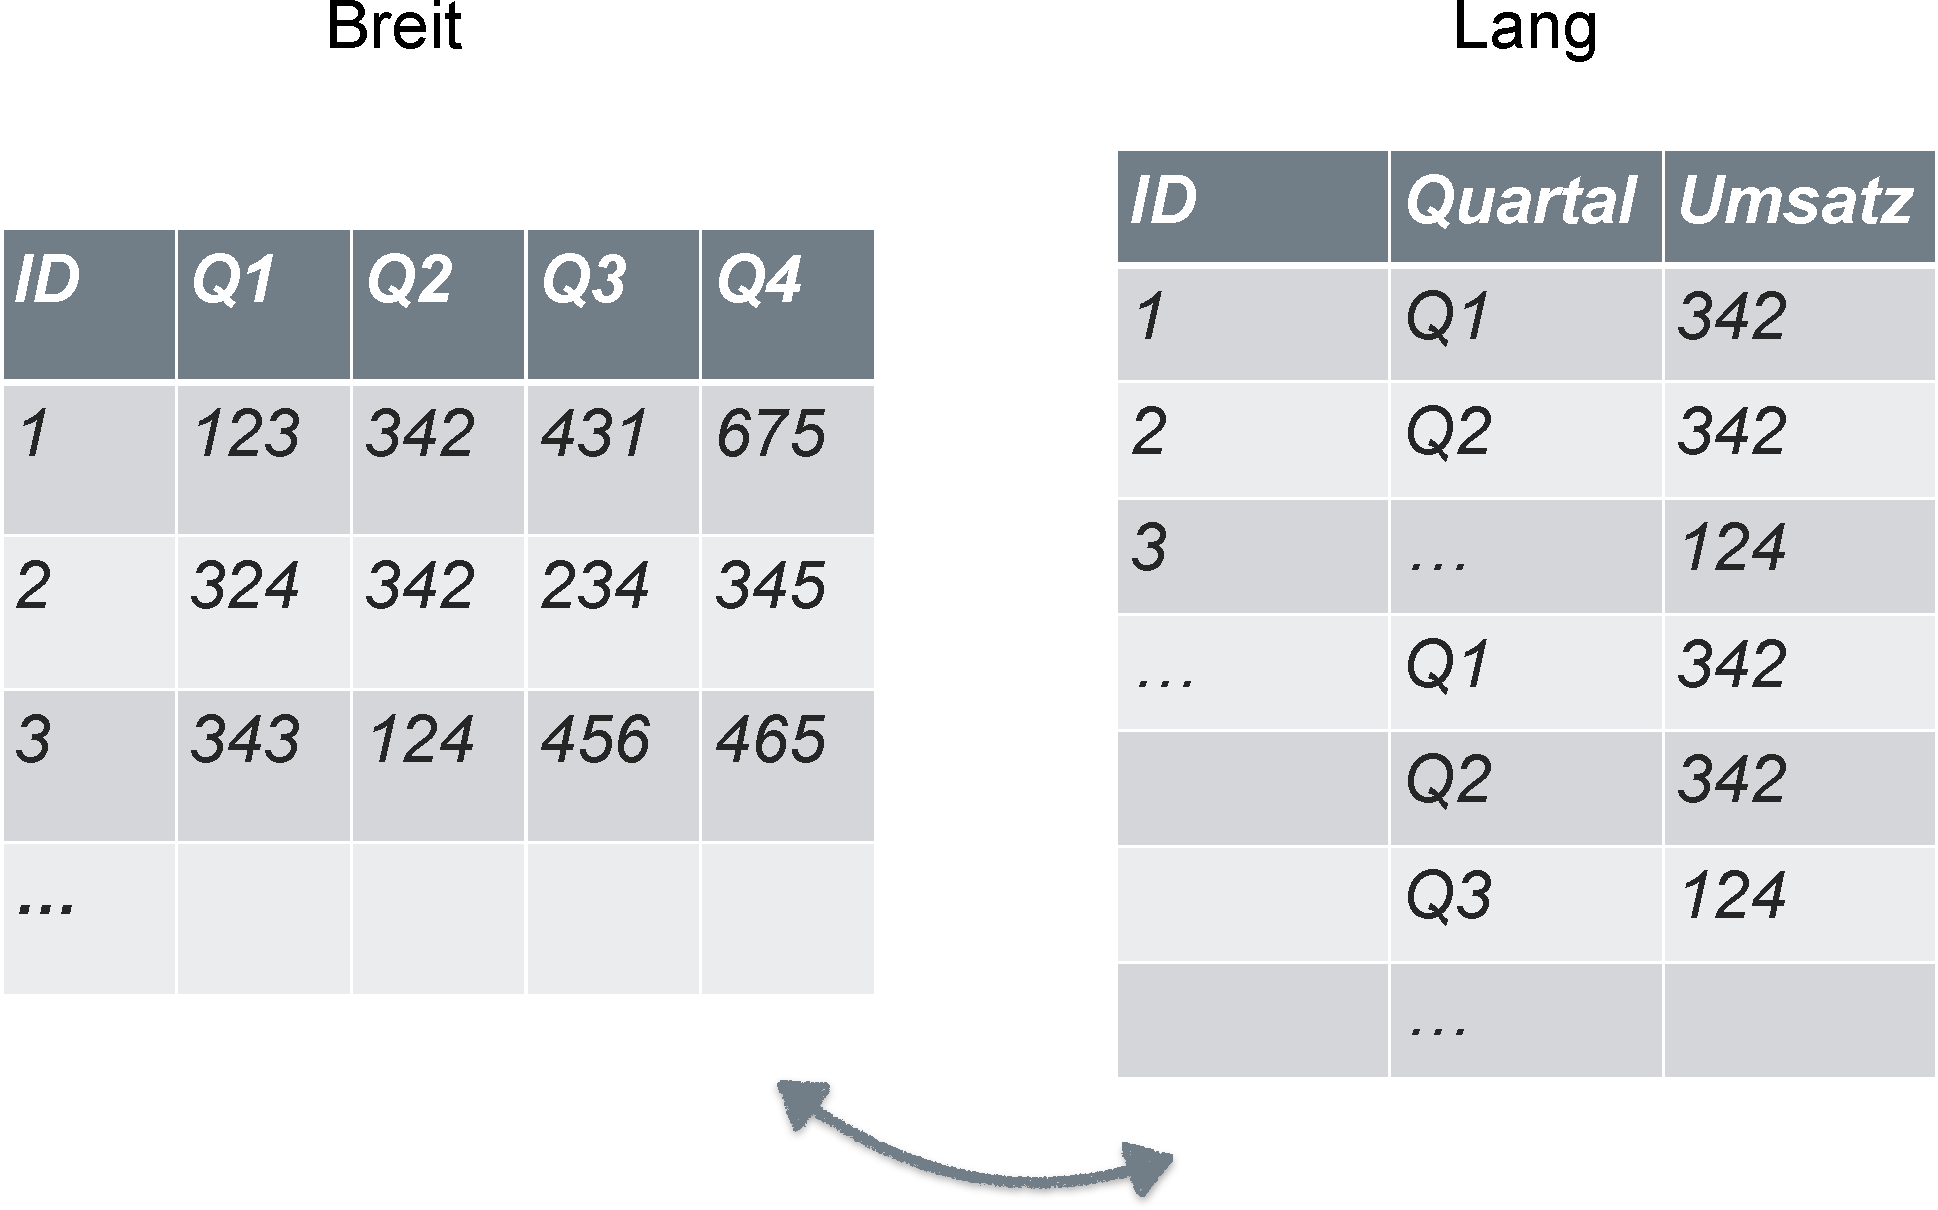
\includegraphics[width=0.7\linewidth]{./images/breit_lang} \end{center}

In der rechten Tabelle sind die Variablen \texttt{Quartal} und
\texttt{Umsatz} klar getrennt; jede hat ihre eigene Spalte. In der
linken Tabelle hingegen sind die beiden Variablen vermischt. Sie haben
nicht mehr ihre eigene Spalte, sondern sind über vier Spalten verteilt.
Die rechte Tabelle ist ein Beispiel für eine Tabelle in Normalform, die
linke nicht.

\begin{figure}

{\centering 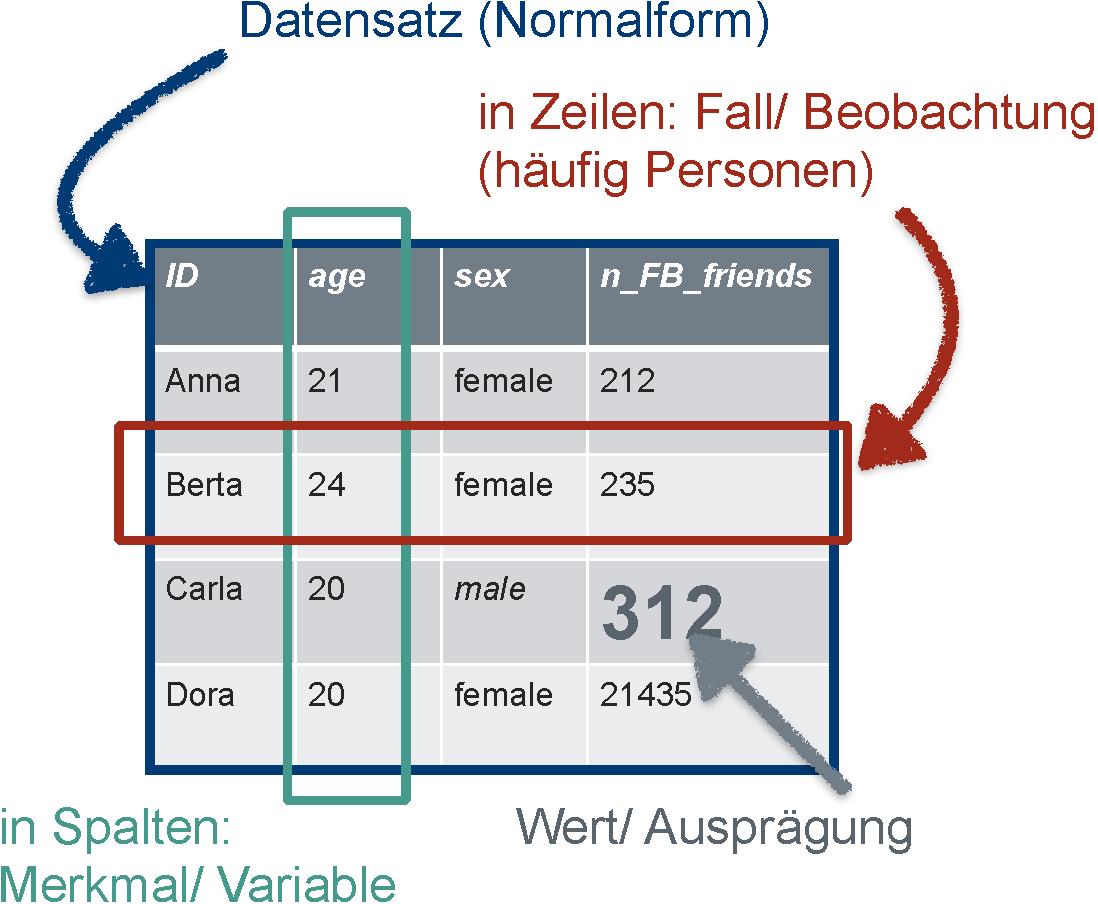
\includegraphics[width=0.7\linewidth]{images/Normalform} 

}

\caption{Illustration eines Datensatzes in Normalform}\label{fig:fig-Normalform}
\end{figure}

Eine der ersten Aktionen einer Datenanalyse sollte also die
``Normalisierung'' Ihrer Tabelle sein. In R bietet sich dazu das Paket
\texttt{tidyr} an, mit dem die Tabelle von Breit- auf Langformat (und
wieder zurück) geschoben werden kann.

Ein Beispiel dazu:

\begin{Shaded}
\begin{Highlighting}[]
\NormalTok{meindf <-}\StringTok{ }\KeywordTok{read.csv}\NormalTok{(}\StringTok{"http://stanford.edu/~ejdemyr/r-tutorials/data/unicef-u5mr.csv"}\NormalTok{)}

\NormalTok{df_lang <-}\StringTok{ }\KeywordTok{gather}\NormalTok{(meindf, year, u5mr, U5MR}\FloatTok{.1950}\NormalTok{:U5MR}\FloatTok{.2015}\NormalTok{)}

\NormalTok{df_lang <-}\StringTok{ }\KeywordTok{separate}\NormalTok{(df_lang, year, }\DataTypeTok{into =} \KeywordTok{c}\NormalTok{(}\StringTok{"U5MR"}\NormalTok{, }\StringTok{"year"}\NormalTok{), }\DataTypeTok{sep =} \StringTok{"."}\NormalTok{)}
\end{Highlighting}
\end{Shaded}

\begin{itemize}
\tightlist
\item
  Die erste Zeile liest die Daten aus einer CSV-Datei ein;
  praktischerweise direkt von einer Webseite.\\
\item
  Die zweite Zeile formt die Daten von breit nach lang um. Die neuen
  Spalten, nach der Umformung heißen dann \texttt{year} und
  \texttt{u5mr} (Sterblichkeit bei Kindern unter fünf Jahren). In die
  Umformung werden die Spalten \texttt{U5MR\ 1950} bis
  \texttt{U5MR\ 2015} einbezogen.
\item
  Die dritte Zeile ``entzerrt'' die Werte der Spalte \texttt{year}; hier
  stehen die ehemaligen Spaltenköpfe. Man nennt sie auch \texttt{key}
  Spalte daher. Steht in einer Zelle von \texttt{year} bspw.
  \texttt{U5MR\ 1950}, so wird \texttt{U5MR} in eine Spalte mit Namen
  \texttt{U5MR} und \texttt{1950} in eine Spalte mit Namen \texttt{year}
  geschrieben.
\end{itemize}

\section{Verweise}\label{verweise-1}

\begin{itemize}
\tightlist
\item
  \emph{R for Data Science} bietet umfangreiche Unterstützung zu diesem
  Thema (Wickham and Grolemund \protect\hyperlink{ref-r4ds}{2016}).
\end{itemize}

\chapter{Daten aufbereiten}\label{daten-aufbereiten}

\begin{figure}

{\centering 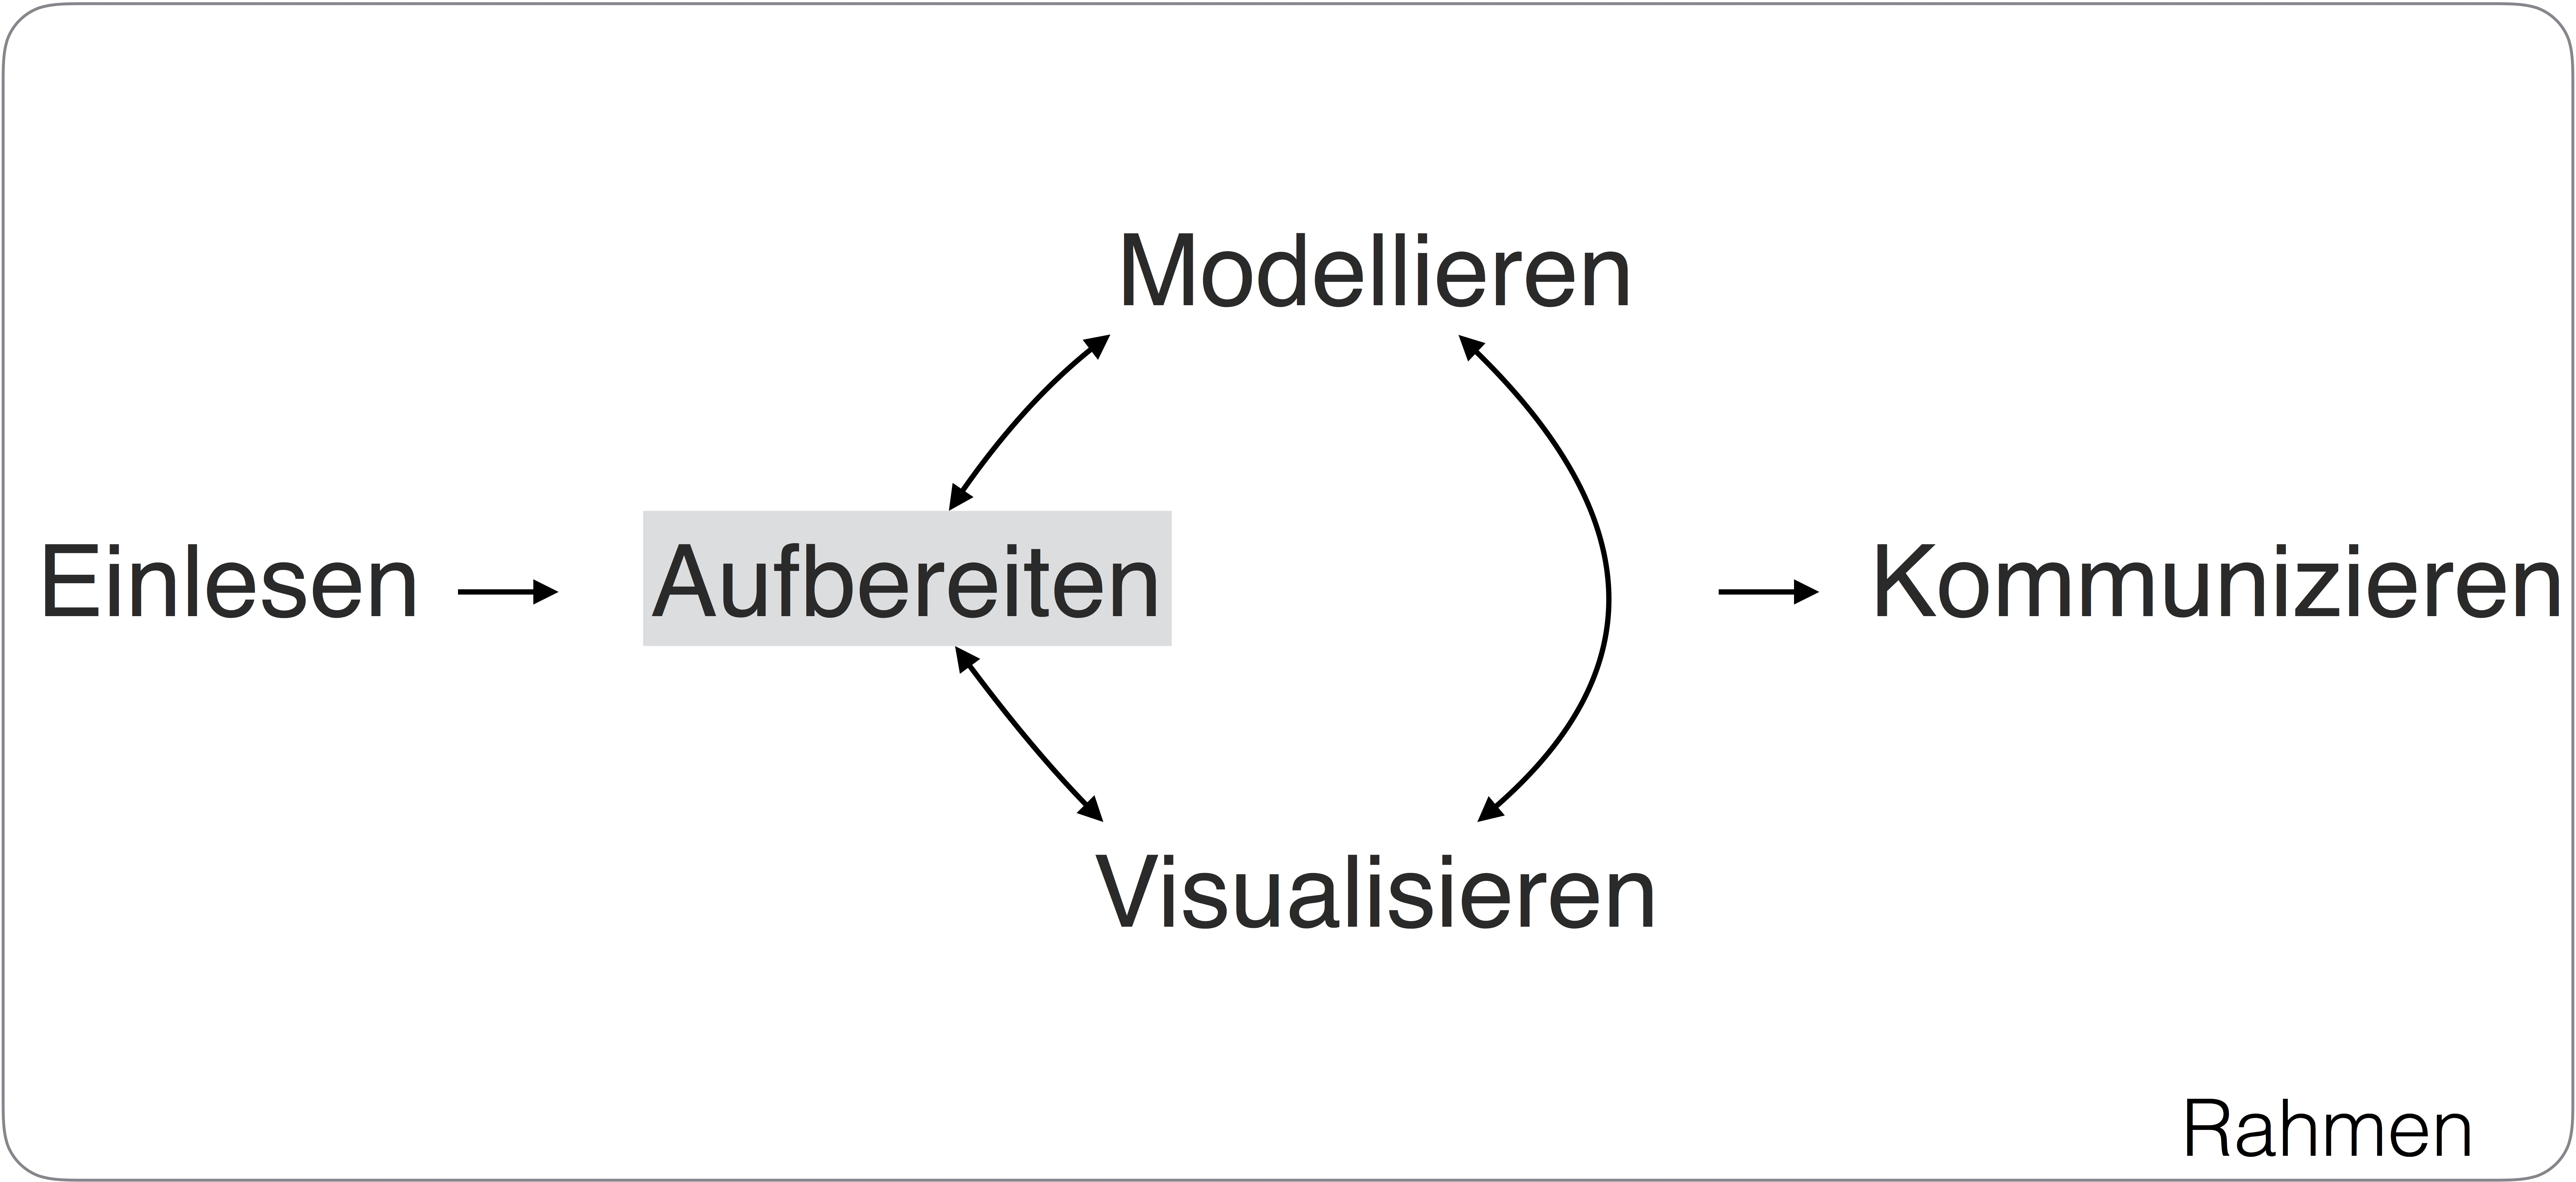
\includegraphics[width=0.7\linewidth]{images/Aufbereiten} 

}

\caption{Daten aufbereiten}\label{fig:unnamed-chunk-2}
\end{figure}

In diesem Kapitel benötigte Pakete:

\begin{Shaded}
\begin{Highlighting}[]
\KeywordTok{library}\NormalTok{(tidyverse)  }\CommentTok{# Datenjudo}
\KeywordTok{library}\NormalTok{(corrr)  }\CommentTok{# Korrelationen berechnen mit der Pfeife}
\KeywordTok{library}\NormalTok{(stringr)   }\CommentTok{# Texte bearbeiten}
\KeywordTok{library}\NormalTok{(car)  }\CommentTok{# für 'recode'}
\KeywordTok{library}\NormalTok{(nycflights13)  }\CommentTok{# Datensatz 'flights'}
\KeywordTok{library}\NormalTok{(knitr)  }\CommentTok{# für HTML-Tabellen}
\KeywordTok{library}\NormalTok{(gridExtra)  }\CommentTok{# für Mehrfachplots}
\end{Highlighting}
\end{Shaded}

Unter Daten aufbereiten im engeren Sinne ist gemeint, die Daten einer
``Grundreinigung'' zu unterziehen, dass sie für weitere Analysen in
geeigneter Form sind. Daten zusammenfassen meint die deskriptive
Statistik; Daten visualisieren ist das Erstellen von Diagrammen. Im
Anschluss kann man die Daten modellieren.

Ist das Explorieren von Daten auch nicht statistisch anspruchsvoll, so
ist es trotzdem von großer Bedeutung und häufig recht zeitintensiv, vor
allem das Daten aufbereiten. Eine Anekdote zur Relevanz der Exploration,
die (so will es die Geschichte) mir an einer Bar nach einer
einschlägigen Konferenz erzählt wurde (daher keine Quellenangebe, Sie
verstehen\ldots{}). Eine Computerwissenschaftlerin aus den USA
(deutschen Ursprungs) hatte einen beeindruckenden ``Track Record'' an
Siegen in Wettkämpfen der Datenanalyse. Tatsächlich hatte sie keine
besonderen, raffinierten Modellierungstechniken eingesetzt; klassische
Regression war ihre Methode der Wahl. Bei einem Wettkampf, bei dem es
darum ging, Krebsfälle aus Krankendaten vorherzusagen (z.B.
Röntgenbildern) fand sie nach langem Datenjudo heraus, dass in die
``ID-Variablen'' Information gesickert war, die dort nicht hingehörte
und die sie nutzen konnte für überraschend (aus Sicht der Mitstreiter)
gute Vorhersagen zu Krebsfällen. Wie war das möglich? Die Daten stammten
aus mehreren Kliniken, jede Klinik verwendete ein anderes System, um IDs
für Patienten zu erstellen. Überall waren die IDs stark genug, um die
Anonymität der Patienten sicherzustellen, aber gleich wohl konnte man
(nach einigem Judo) unterscheiden, welche ID von welcher Klinik stammte.
Was das bringt? Einige Kliniken waren reine Screening-Zentren, die die
Normalbevölkerung versorgte. Dort sind wenig Krebsfälle zu erwarten.
Andere Kliniken jedoch waren Onkologie-Zentren für bereits bekannte
Patienten oder für Patienten mit besonderer Risikolage. Wenig
überraschen, dass man dann höhere Krebsraten vorhersagen kann.
Eigentlich ganz einfach; besondere Mathe steht hier (zumindest in dieser
Geschichte) nicht dahinter. Und, wenn man den Trick kennt, ganz einfach.
Aber wie so oft ist es nicht leicht, den Trick zu finden. Sorgfältiges
Datenjudo hat hier den Schlüssel zum Erfolg gebracht.

\section{Typische Probleme}\label{typische-probleme}

Bevor man seine Statistik-Trickkiste so richtig schön aufmachen kann,
muss man die Daten häufig erst noch in Form bringen. Das ist nicht
schwierig in dem Sinne, dass es um komplizierte Mathe ginge. Allerdings
braucht es mitunter recht viel Zeit und ein paar (oder viele)
handwerkliche Tricks sind hilfreich. Hier soll das folgende Kapitel
helfen.

Mit ``Datenjudo'' (ein Fachbegriff aus der östlichen Zahlentheorie) ist
gemeint, die Daten so ``umzuformen'', ``aufzubereiten'', oder
``reinigen'' , dass sie passend für statistische Analysen sind.

Typische Probleme, die immer wieder auftreten, sind:

\begin{itemize}
\tightlist
\item
  Fehlende Werte: Irgend jemand hat auf eine meiner schönen Fragen in
  der Umfrage nicht geantwortet!
\item
  Unerwartete Daten: Auf die Frage, wie viele Facebook-Freunde er oder
  sie habe, schrieb die Person ``I like you a lot''. Was tun???
\item
  Daten müssen umgeformt werden: Für jede der beiden Gruppen seiner
  Studie hat Joachim einen Google-Forms-Fragebogen aufgesetzt. Jetzt hat
  er zwei Tabellen, die er ``verheiraten'' möchte. Geht das?
\item
  Neue Spalten berechnen: Ein Student fragt nach der Anzahl der
  richtigen Aufgaben in der Statistik-Probeklausur. Wir wollen helfen
  und im entsprechenden Datensatz eine Spalte erzeugen, in der pro
  Person die Anzahl der richtig beantworteten Fragen steht.
\end{itemize}

\section{\texorpdfstring{Daten aufbereiten mit
\texttt{dplyr}}{Daten aufbereiten mit dplyr}}\label{daten-aufbereiten-mit-dplyr}

Es gibt viele Möglichkeiten, Daten mit R aufzubereiten; \texttt{dplyr}
ist ein populäres Paket dafür. Eine zentrale Idee von \texttt{dplyr}
ist, dass es nur ein paar wenige Grundbausteine geben sollte, die sich
gut kombinieren lassen. Sprich: Wenige grundlegende Funktionen mit eng
umgrenzter Funktionalität. Der Autor, Hadley Wickham, sprach einmal in
einem Forum (citation needed), dass diese Befehle wenig können, das
Wenige aber gut. Ein Nachteil dieser Konzeption kann sein, dass man
recht viele dieser Bausteine kombinieren muss, um zum gewünschten
Ergebnis zu kommen. Außerdem muss man die Logik des Baukastens gut
verstanden habe - die Lernkurve ist also erstmal steiler. Dafür ist man
dann nicht darauf angewiesen, dass es irgendwo ``Mrs Right'' gibt, die
genau das kann, so wie ich das will. Außerdem braucht man sich auch
nicht viele Funktionen merken. Es reicht einen kleinen Satz an
Funktionen zu kennen (die praktischerweise konsistent in Syntax und
Methodik sind).

Willkommen in der Welt von \texttt{dyplr}! \texttt{dplyr} hat seinen
Namen, weil es sich ausschließlich um \emph{D}ataframes bemüht; es
erwartet einen Dataframe als Eingabe und gibt einen Dataframe zurück
(zumindest bei den meisten Befehlen).

Diese Bausteine sind typische Tätigkeiten im Umgang mit Daten; nichts
Überraschendes. Schauen wir uns diese Bausteine näher an.

\subsection{\texorpdfstring{Zeilen filtern mit
\texttt{filter}}{Zeilen filtern mit filter}}\label{zeilen-filtern-mit-filter}

Häufig will man bestimmte Zeilen aus einer Tabelle filtern. Zum Beispiel
man arbeitet für die Zigarettenindustrie und ist nur an den Rauchern
interessiert (die im Übrigen unser Gesundheitssystem retten (Krämer
\protect\hyperlink{ref-kraemer2011wir}{2011})), nicht an Nicht-Rauchern;
es sollen die nur Umsatzzahlen des letzten Quartals untersucht werden,
nicht die vorherigen Quartale; es sollen nur die Daten aus Labor X
(nicht Labor Y) ausgewertet werden etc.

Ein Sinnbild:

\begin{figure}

{\centering 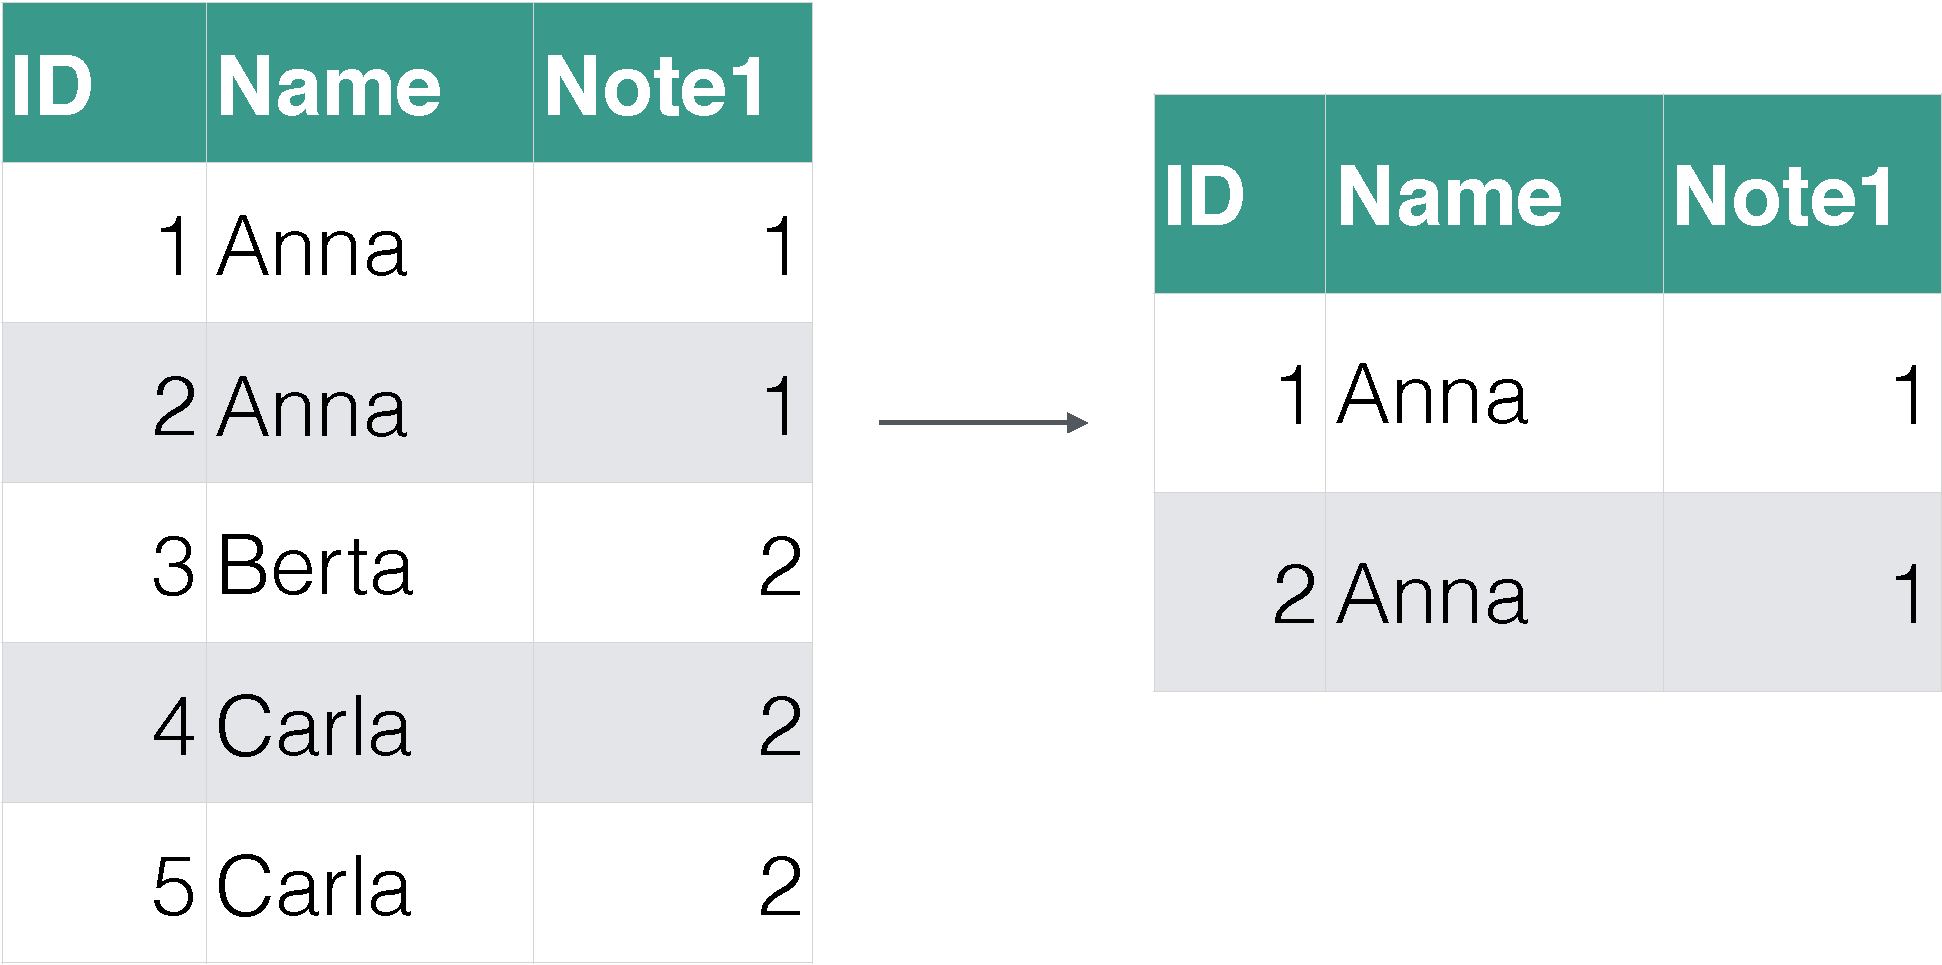
\includegraphics[width=0.7\linewidth]{./images/filter} 

}

\caption{Zeilen filtern}\label{fig:fig-filter}
\end{figure}

Merke:

\begin{quote}
Die Funktion \texttt{filter} filtert Zeilen aus einem Dataframe.
\end{quote}

Schauen wir uns einige Beispiel an; zuerst die Daten laden nicht
vergessen. Achtung: ``Wohnen'' die Daten in einem Paket, muss dieses
Paket installiert sein, damit man auf die Daten zugreifen kann.

\begin{Shaded}
\begin{Highlighting}[]
\KeywordTok{data}\NormalTok{(profiles, }\DataTypeTok{package =} \StringTok{"okcupiddata"}\NormalTok{)  }\CommentTok{# Das Paket muss installiert sein}
\end{Highlighting}
\end{Shaded}

\begin{Shaded}
\begin{Highlighting}[]
\NormalTok{df_frauen <-}\StringTok{ }\KeywordTok{filter}\NormalTok{(profiles, sex ==}\StringTok{ "f"}\NormalTok{)  }\CommentTok{# nur die Frauen}
\NormalTok{df_alt <-}\StringTok{ }\KeywordTok{filter}\NormalTok{(profiles, age >}\StringTok{ }\DecValTok{70}\NormalTok{)  }\CommentTok{# nur die alten}
\NormalTok{df_alte_frauen <-}\StringTok{ }\KeywordTok{filter}\NormalTok{(profiles, age >}\StringTok{ }\DecValTok{70}\NormalTok{, sex ==}\StringTok{ "f"}\NormalTok{)  }\CommentTok{# nur die alten Frauen, d.h. UND-Verknüpfung}
\NormalTok{df_nosmoke_nodrinks <-}\StringTok{ }\KeywordTok{filter}\NormalTok{(profiles, smokes ==}\StringTok{ "no"} \NormalTok{|}\StringTok{ }\NormalTok{drinks ==}\StringTok{ "not at all"}\NormalTok{) }
\CommentTok{# liefert alle Personen, die Nicht-Raucher *oder* Nicht-Trinker sind}
\end{Highlighting}
\end{Shaded}

Gar nicht so schwer, oder? Allgemeiner gesprochen werden diejenigen
Zeilen gefiltert (also behalten bzw. zurückgeliefert), für die das
Filterkriterium \texttt{TRUE} ist.

\BeginKnitrBlock{rmdcaution}
Manche Befehle wie \texttt{filter} haben einen Allerweltsnamen; gut
möglich, dass ein Befehl mit gleichem Namen in einem anderen (geladenen)
Paket existiert. Das kann dann zu Verwirrungen führen - und kryptischen
Fehlern. Im Zweifel den Namen des richtigen Pakets ergänzen, und zwar
zum Beispiel so: \texttt{dplyr::filter(...)}.
\EndKnitrBlock{rmdcaution}

Einige fortgeschrittene Beispiele für \texttt{filter}:

Man kann alle Elemente (Zeilen) filtern, die zu einer Menge gehören und
zwar mit diesem Operator: \texttt{\%in\%}:

\begin{Shaded}
\begin{Highlighting}[]
\KeywordTok{filter}\NormalTok{(profiles, body_type %in%}\StringTok{ }\KeywordTok{c}\NormalTok{(}\StringTok{"a little extra"}\NormalTok{, }\StringTok{"average"}\NormalTok{))}
\end{Highlighting}
\end{Shaded}

Besonders Textdaten laden zu einigen Extra-Überlegungen ein; sagen wir,
wir wollen alle Personen filtern, die Katzen bei den Haustieren
erwähnen. Es soll reichen, wenn \texttt{cat} ein Teil des Textes ist;
also \texttt{likes\ dogs\ and\ likes\ cats} wäre OK (soll gefiltert
werden). Dazu nutzen wir ein Paket zur Bearbeitung von Strings
(Textdaten):

\begin{Shaded}
\begin{Highlighting}[]

\KeywordTok{filter}\NormalTok{(profiles, }\KeywordTok{str_detect}\NormalTok{(pets, }\StringTok{"cats"}\NormalTok{))}
\end{Highlighting}
\end{Shaded}

Ein häufiger Fall ist, Zeilen \emph{ohne} fehlende Werte (\texttt{NA}s)
zu filtern. Das geht einfach:

\begin{Shaded}
\begin{Highlighting}[]
\NormalTok{profiles_keine_nas <-}\StringTok{ }\KeywordTok{na.omit}\NormalTok{(profiles)}
\end{Highlighting}
\end{Shaded}

Aber was ist, wenn wir nur bei bestimmten Spalten wegen fehlender Werte
besorgt sind? Sagen wir bei \texttt{income} und bei \texttt{sex}:

\begin{Shaded}
\begin{Highlighting}[]
\KeywordTok{filter}\NormalTok{(profiles, !}\KeywordTok{is.na}\NormalTok{(income) |}\StringTok{ }\NormalTok{!}\KeywordTok{is.na}\NormalTok{(sex))}
\end{Highlighting}
\end{Shaded}

\subsection{\texorpdfstring{Spalten wählen mit
\texttt{select}}{Spalten wählen mit select}}\label{spalten-wahlen-mit-select}

Das Gegenstück zu \texttt{filter} ist \texttt{select}; dieser Befehl
liefert die gewählten Spalten zurück. Das ist häufig praktisch, wenn der
Datensatz sehr ``breit'' ist, also viele Spalten enthält. Dann kann es
übersichtlicher sein, sich nur die relevanten auszuwählen. Das Sinnbild
für diesen Befehl:

\begin{figure}

{\centering 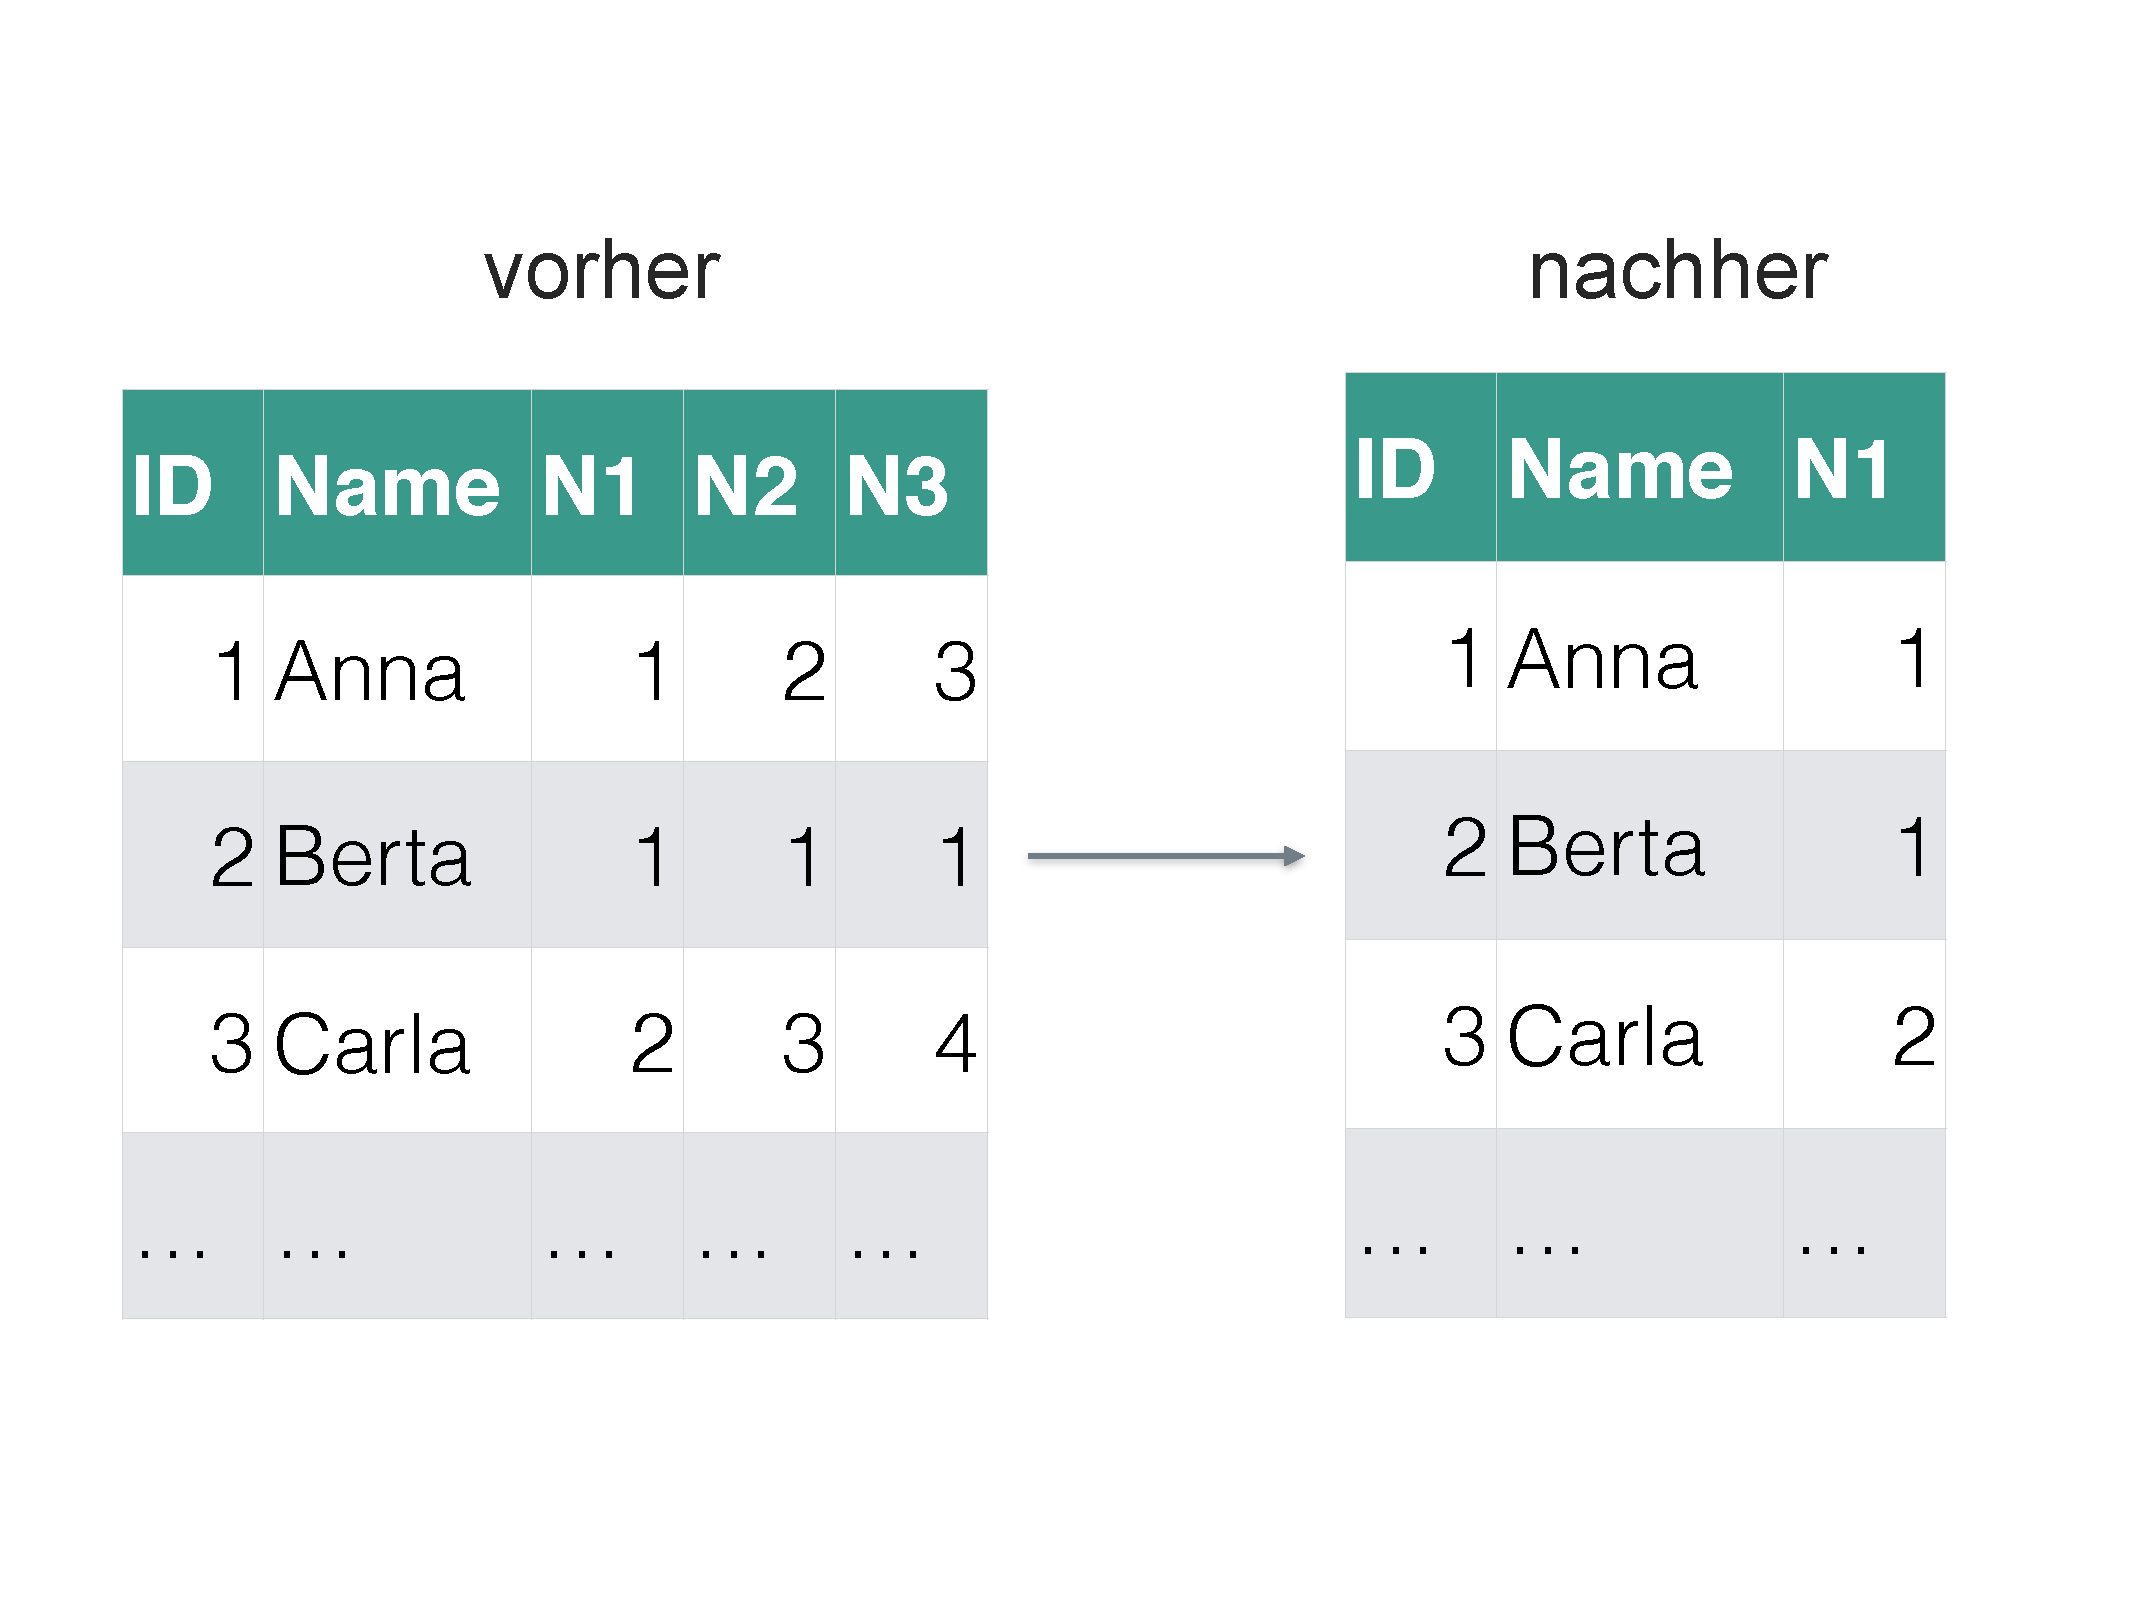
\includegraphics[width=0.7\linewidth]{images/select} 

}

\caption{Spalten auswählen}\label{fig:fig-select}
\end{figure}

Merke:

\begin{quote}
Die Funktion select wählt Spalten aus einem Dataframe aus.
\end{quote}

\begin{Shaded}
\begin{Highlighting}[]
\NormalTok{if (!}\KeywordTok{file.exists}\NormalTok{(}\StringTok{"./data/test_inf_short.csv"}\NormalTok{)) \{}
  \NormalTok{stats_test <-}\StringTok{ }\KeywordTok{read.csv}\NormalTok{(}\StringTok{"https://sebastiansauer.github.io/data/test_inf_short.csv"}\NormalTok{) }
\NormalTok{\} else \{}
  \NormalTok{stats_test <-}\StringTok{ }\KeywordTok{read.csv}\NormalTok{(}\StringTok{"./data/test_inf_short.csv"}\NormalTok{)}
\NormalTok{\}}
\end{Highlighting}
\end{Shaded}

Hier haben wir erst geprüft, ob die Datei \texttt{test\_inf\_short.csv}
existiert; falls nein, laden wir sie herunter. Andernfalls lesen wir sie
aus dem lokalen Verzeichnis.

\begin{Shaded}
\begin{Highlighting}[]
\KeywordTok{select}\NormalTok{(stats_test, score)  }\CommentTok{# Spalte `score` auswählen}
\KeywordTok{select}\NormalTok{(stats_test, score, study_time)  }\CommentTok{# Splaten `score` und `study_time` auswählen}
\KeywordTok{select}\NormalTok{(stats_test, score:study_time) }\CommentTok{# dito}
\KeywordTok{select}\NormalTok{(stats_test, }\DecValTok{5}\NormalTok{:}\DecValTok{6}\NormalTok{) Spalten }\DecValTok{5} \NormalTok{bis }\DecValTok{6} \NormalTok{auswählen}
\end{Highlighting}
\end{Shaded}

Tatsächlich ist der Befehl \texttt{select} sehr flexibel; es gibt viele
Möglichkeiten, Spalten auszuwählen. Im \texttt{dplyr}-Cheatsheet findet
sich ein guter Überblick dazu.

\subsection{\texorpdfstring{Zeilen sortieren mit
\texttt{arrange}}{Zeilen sortieren mit arrange}}\label{zeilen-sortieren-mit-arrange}

Man kann zwei Arten des Umgangs mit R unterscheiden: Zum einen der
``interaktive Gebrauch'' und zum anderen ``richtiges Programmieren''. Im
interaktiven Gebrauch geht es uns darum, die Fragen zum aktuell
vorliegenden Datensatz (schnell) zu beantworten. Es geht nicht darum,
eine allgemeine Lösung zu entwickeln, die wir in die Welt verschicken
können und die dort ein bestimmtes Problem löst, ohne dass der
Entwickler (wir) dabei Hilfestellung geben muss. ``Richtige'' Software,
wie ein R-Paket oder Microsoft Powerpoint, muss diese Erwartung
erfüllen; ``richtiges Programmieren'' ist dazu vonnöten. Natürlich sind
in diesem Fall die Ansprüche an die Syntax (der ``Code'', hört sich
cooler an) viel höher. In dem Fall muss man alle Eventualitäten
voraussehen und sicherstellen, dass das Programm auch beim
merkwürdigsten Nutzer brav seinen Dienst tut. Wir haben hier, beim
interaktiven Gebrauch, niedrigere Ansprüche bzw. andere Ziele.

Beim interaktiven Gebrauch von R (oder beliebigen Analyseprogrammen) ist
das Sortieren von Zeilen eine recht häufige Tätigkeit. Typisches
Beispiel wäre der Lehrer, der eine Tabelle mit Noten hat und wissen
will, welche Schüler die schlechtesten oder die besten sind in einem
bestimmten Fach. Oder bei der Prüfung der Umsätze nach Filialen möchten
wir die umsatzstärksten sowie -schwächsten Niederlassungen kennen.

Ein R-Befehl hierzu ist \texttt{arrange}; einige Beispiele zeigen die
Funktionsweise am besten:

\begin{Shaded}
\begin{Highlighting}[]

\KeywordTok{arrange}\NormalTok{(stats_test, score)  %>%}\StringTok{ }\KeywordTok{head}\NormalTok{() }\CommentTok{# liefert die *schlechtesten* Noten zurück}
\CommentTok{#>     X                 V_1 study_time self_eval interest score}
\CommentTok{#> 1 234 23.01.2017 18:13:15          3         1        1    17}
\CommentTok{#> 2   4 06.01.2017 09:58:05          2         3        2    18}
\CommentTok{#> 3 131 19.01.2017 18:03:45          2         3        4    18}
\CommentTok{#> 4 142 19.01.2017 19:02:12          3         4        1    18}
\CommentTok{#> 5  35 12.01.2017 19:04:43          1         2        3    19}
\CommentTok{#> 6  71 15.01.2017 15:03:29          3         3        3    20}
\KeywordTok{arrange}\NormalTok{(stats_test, -score) %>%}\StringTok{ }\KeywordTok{head}\NormalTok{() }\CommentTok{# liefert die *besten* Noten zurück}
\CommentTok{#>    X                 V_1 study_time self_eval interest score}
\CommentTok{#> 1  3 05.01.2017 23:33:47          5        10        6    40}
\CommentTok{#> 2  7 06.01.2017 14:25:49         NA        NA       NA    40}
\CommentTok{#> 3 29 12.01.2017 09:48:16          4        10        3    40}
\CommentTok{#> 4 41 13.01.2017 12:07:29          4        10        3    40}
\CommentTok{#> 5 58 14.01.2017 15:43:01          3         8        2    40}
\CommentTok{#> 6 83 16.01.2017 10:16:52         NA        NA       NA    40}
\KeywordTok{arrange}\NormalTok{(stats_test, interest, score) %>%}\StringTok{ }\KeywordTok{head}\NormalTok{()}
\CommentTok{#>     X                 V_1 study_time self_eval interest score}
\CommentTok{#> 1 234 23.01.2017 18:13:15          3         1        1    17}
\CommentTok{#> 2 142 19.01.2017 19:02:12          3         4        1    18}
\CommentTok{#> 3 221 23.01.2017 11:40:30          1         1        1    23}
\CommentTok{#> 4 230 23.01.2017 16:27:49          1         1        1    23}
\CommentTok{#> 5  92 17.01.2017 17:18:55          1         1        1    24}
\CommentTok{#> 6 107 18.01.2017 16:01:36          3         2        1    24}
\end{Highlighting}
\end{Shaded}

Einige Anmerkungen. Die generelle Syntax lautet
\texttt{arrange(df,\ Spalte1,\ ...)}, wobei \texttt{df} den Dataframe
bezeichnet und \texttt{Spalte1} die erste zu sortierende Spalte; die
Punkte \texttt{...} geben an, dass man weitere Parameter übergeben kann.
Am wichtigsten ist hier, dass man weitere Spalten übergeben kann. Dazu
gleich mehr.

Standardmäßig sortiert \texttt{arrange} \emph{aufsteigend} (weil kleine
Zahlen im Zahlenstrahl vor den großen Zahlen kommen). Möchte man diese
Reihenfolge umdrehen (große Werte zuert), so kann man ein Minuszeichen
vor den Namen der Spalte setzen.

Gibt man \emph{zwei oder mehr} Spalten an, so werden pro Wert von
\texttt{Spalte1} die Werte von \texttt{Spalte2} sortiert etc; man
betrachte den Output des Beispiels oben dazu.

Aber was heißt dieses komisch Symbol: \texttt{\%\textgreater{}\%}? Diese
sogenannte ``Pfeife'' lässt sich mit ``und dann'' ins Deutshce
übersetzen. Also:

\begin{verbatim}
sortiere(diese_Tabelle, nach_dieser_Spalte) UND DANN zeig_die_ersten_Zeilen
\end{verbatim}

Der Befehl \texttt{head} zeigt dier ersten paar Zeilen eines
Dataframes.\footnote{In der Regel 10 Zeilen, wobei ich irgendwo
  versteckt gesagt habe, es sollen nur 6 Zeilen am Bildschirm gedruckt
  werden.}

Merke:

\begin{quote}
Die Funktion arrange sortiert die Zeilen eines Datafames.
\end{quote}

Ein Sinnbild zur Verdeutlichung:

\begin{figure}

{\centering 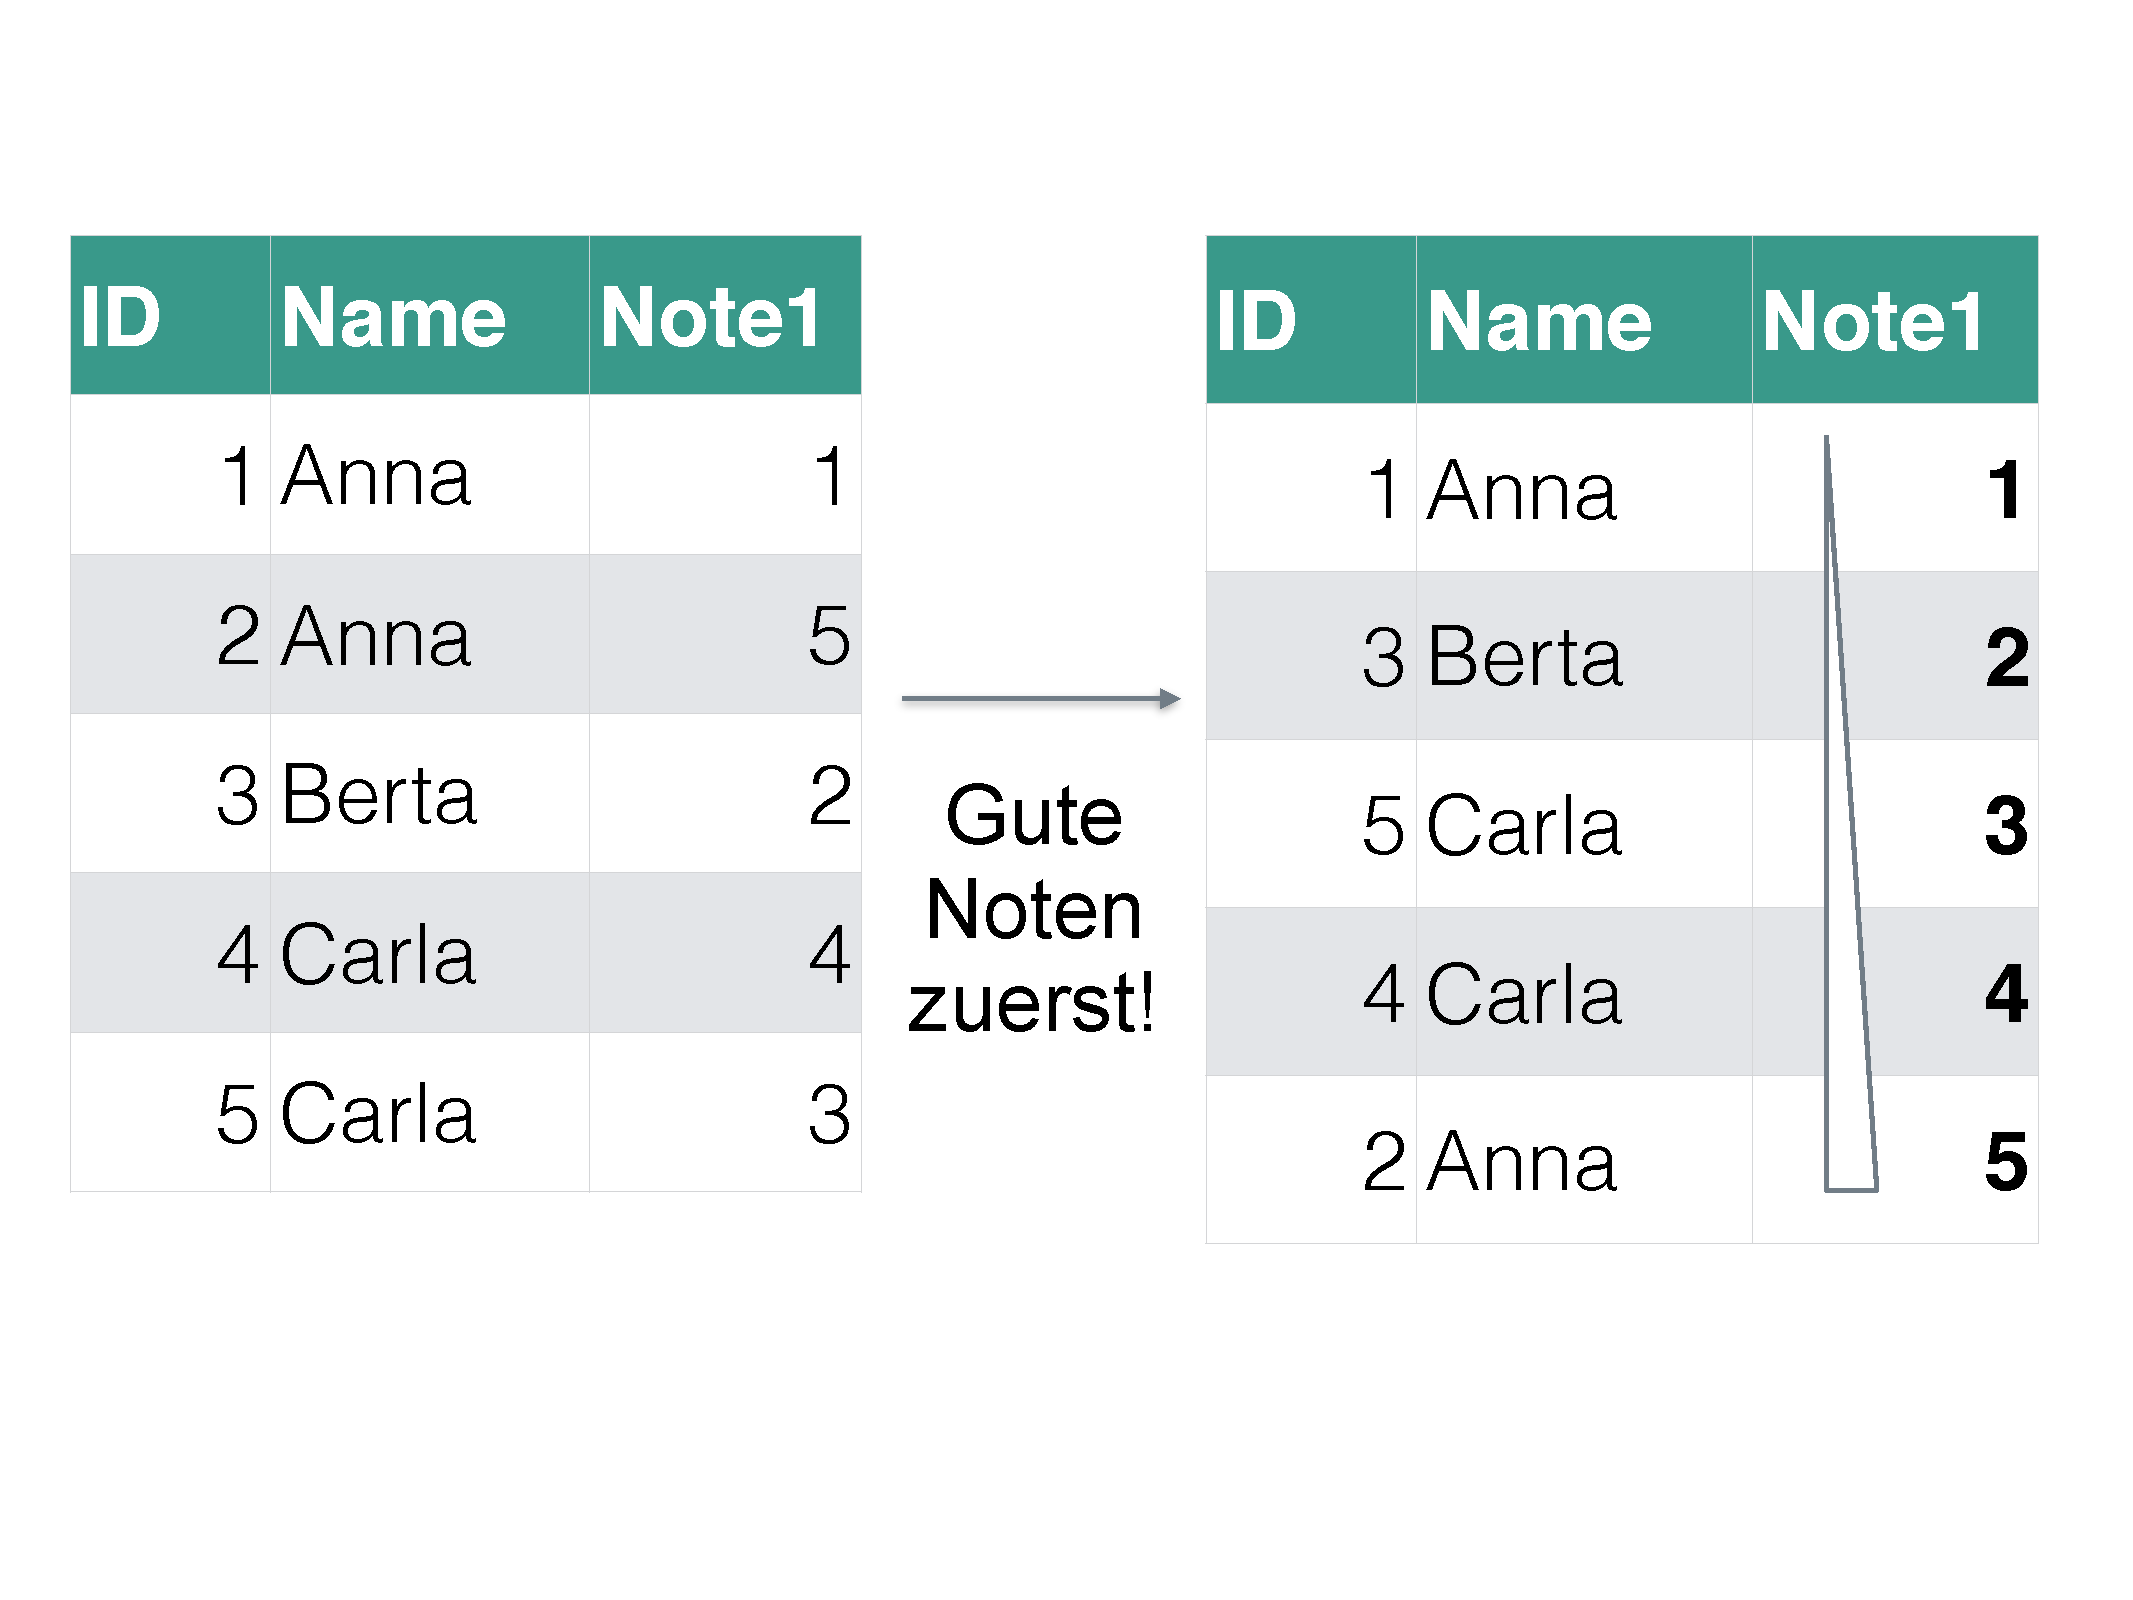
\includegraphics[width=0.7\linewidth]{./images/arrange} 

}

\caption{Spalten sortieren}\label{fig:fig-arrange}
\end{figure}

Ein ähnliches Ergebnis erhält mit man \texttt{top\_n()}, welches die
\texttt{n} \emph{größten} \emph{Ränge} widergibt:

\begin{Shaded}
\begin{Highlighting}[]

\KeywordTok{top_n}\NormalTok{(stats_test, }\DecValTok{3}\NormalTok{)}
\CommentTok{#>      X                 V_1 study_time self_eval interest score}
\CommentTok{#> 1    3 05.01.2017 23:33:47          5        10        6    40}
\CommentTok{#> 2    7 06.01.2017 14:25:49         NA        NA       NA    40}
\CommentTok{#> 3   29 12.01.2017 09:48:16          4        10        3    40}
\CommentTok{#> 4   41 13.01.2017 12:07:29          4        10        3    40}
\CommentTok{#> 5   58 14.01.2017 15:43:01          3         8        2    40}
\CommentTok{#> 6   83 16.01.2017 10:16:52         NA        NA       NA    40}
\CommentTok{#> 7  116 18.01.2017 23:07:32          4         8        5    40}
\CommentTok{#> 8  119 19.01.2017 09:05:01         NA        NA       NA    40}
\CommentTok{#> 9  132 19.01.2017 18:22:32         NA        NA       NA    40}
\CommentTok{#> 10 175 20.01.2017 23:03:36          5        10        5    40}
\CommentTok{#> 11 179 21.01.2017 07:40:05          5         9        1    40}
\CommentTok{#> 12 185 21.01.2017 15:01:26          4        10        5    40}
\CommentTok{#> 13 196 22.01.2017 13:38:56          4        10        5    40}
\CommentTok{#> 14 197 22.01.2017 14:55:17          4        10        5    40}
\CommentTok{#> 15 248 24.01.2017 16:29:45          2        10        2    40}
\CommentTok{#> 16 249 24.01.2017 17:19:54         NA        NA       NA    40}
\CommentTok{#> 17 257 25.01.2017 10:44:34          2         9        3    40}
\CommentTok{#> 18 306 27.01.2017 11:29:48          4         9        3    40}
\KeywordTok{top_n}\NormalTok{(stats_test, }\DecValTok{3}\NormalTok{, interest)}
\CommentTok{#>     X                 V_1 study_time self_eval interest score}
\CommentTok{#> 1   3 05.01.2017 23:33:47          5        10        6    40}
\CommentTok{#> 2   5 06.01.2017 14:13:08          4         8        6    34}
\CommentTok{#> 3  43 13.01.2017 14:14:16          4         8        6    36}
\CommentTok{#> 4  65 15.01.2017 12:41:27          3         6        6    22}
\CommentTok{#> 5 110 18.01.2017 18:53:02          5         8        6    37}
\CommentTok{#> 6 136 19.01.2017 18:22:57          3         1        6    39}
\CommentTok{#> 7 172 20.01.2017 20:42:46          5        10        6    34}
\CommentTok{#> 8 214 22.01.2017 21:57:36          2         6        6    31}
\CommentTok{#> 9 301 27.01.2017 08:17:59          4         8        6    33}
\end{Highlighting}
\end{Shaded}

Gibt man \emph{keine} Spalte an, so bezieht sich \texttt{top\_n} auf die
letzte Spalte im Datensatz.

Da sich hier mehrere Personen den größten Rang (Wert 40) teilen,
bekommen wir \emph{nicht} 3 Zeilen zurückgeliefert, sondern entsprechend
mehr.

\subsection{\texorpdfstring{Datensatz gruppieren mit
\texttt{group\_by}}{Datensatz gruppieren mit group\_by}}\label{datensatz-gruppieren-mit-group_by}

Einen Datensatz zu gruppieren ist ebenfalls eine häufige Angelegenheit:
Was ist der mittlere Umsatz in Region X im Vergleich zu Region Y? Ist
die Reaktionszeit in der Experimentalgruppe kleiner als in der
Kontrollgruppe? Können Männer schneller ausparken als Frauen? Man sieht,
dass das Gruppieren v.a. in Verbindung mit Mittelwerten oder anderen
Zusammenfassungen sinnvol ist; dazu im nächsten Abschnitt mehr.

\begin{figure}

{\centering 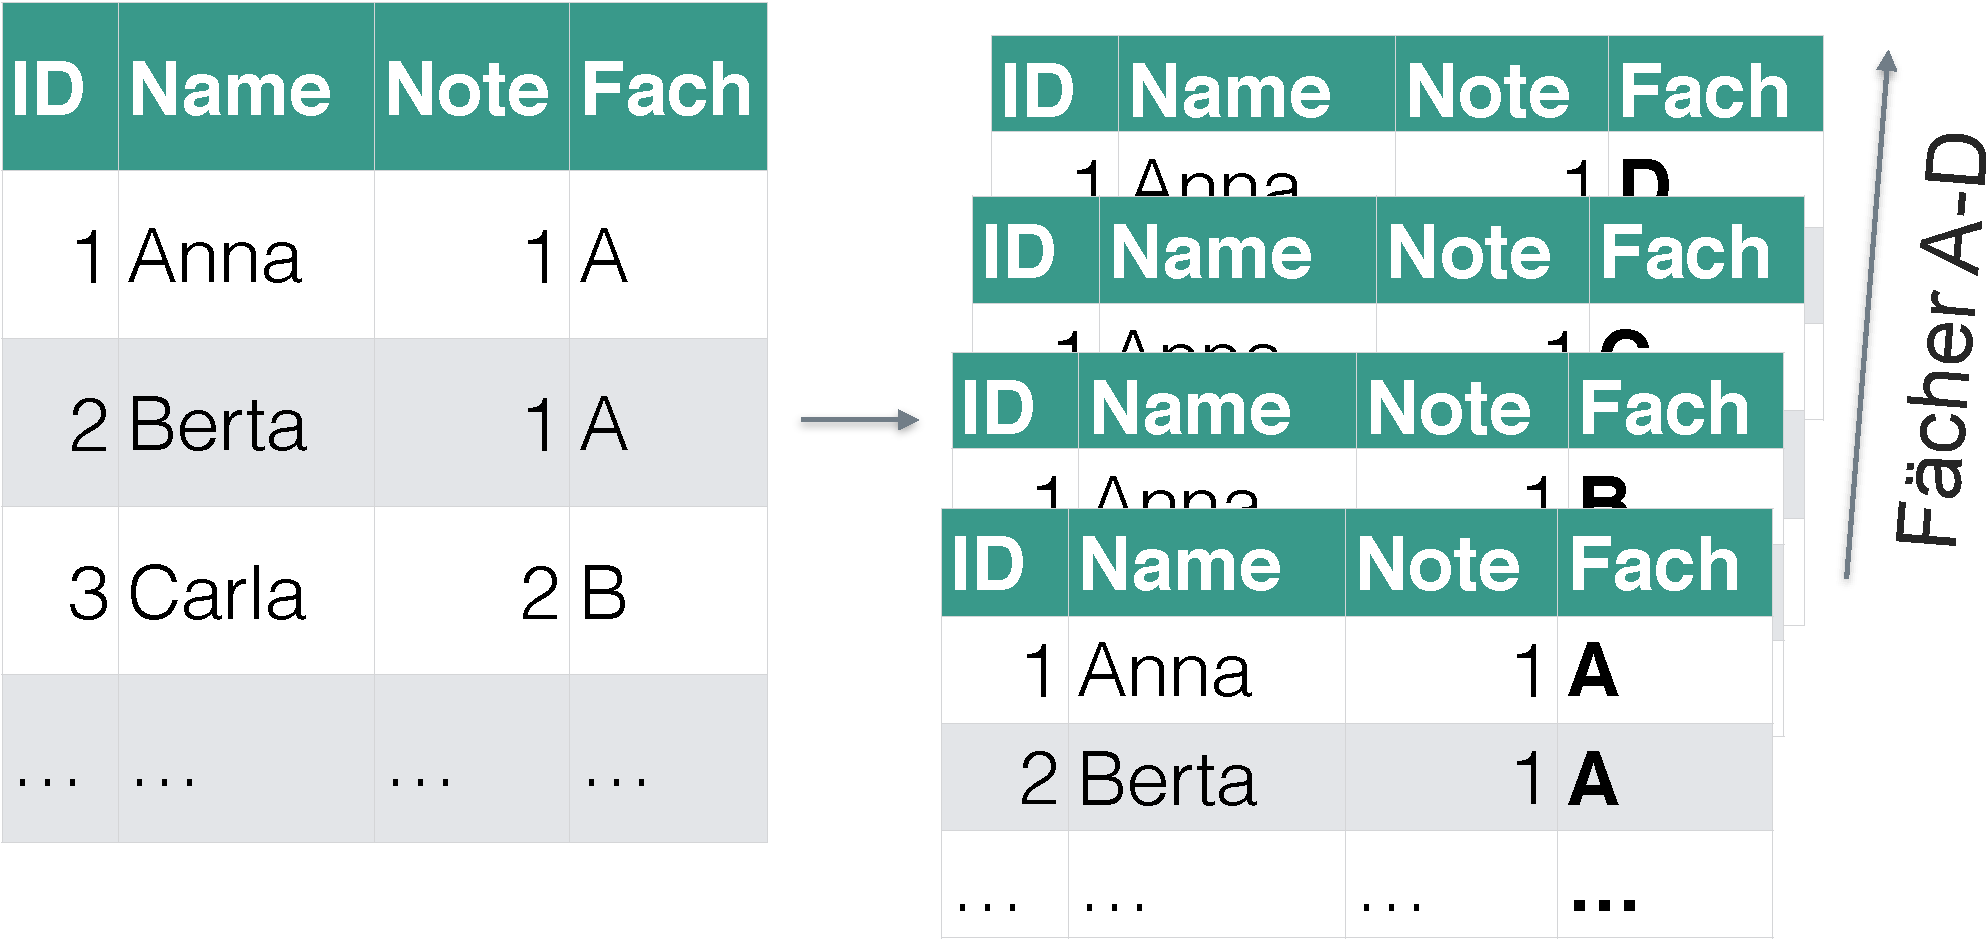
\includegraphics[width=0.7\linewidth]{./images/group_by} 

}

\caption{Datensätze nach Subgruppen aufteilen}\label{fig:fig-groupby}
\end{figure}

In der Abbildung wurde der Datensatz anhand der Spalte \texttt{Fach} in
mehrere Gruppen geteilt. Wir könnten uns als nächstes z.B. Mittelwerte
pro Fach - d.h. pro Gruppe (pro Ausprägung von \texttt{Fach}) - ausgeben
lassen; in diesem Fall vier Gruppen (Fach A bis D).

\begin{Shaded}
\begin{Highlighting}[]
\NormalTok{test_gruppiert <-}\StringTok{ }\KeywordTok{group_by}\NormalTok{(stats_test, interest)}
\NormalTok{test_gruppiert}
\CommentTok{#> Source: local data frame [306 x 6]}
\CommentTok{#> Groups: interest [7]}
\CommentTok{#> }
\CommentTok{#>        X                 V_1 study_time self_eval interest score}
\CommentTok{#>    <int>              <fctr>      <int>     <int>    <int> <int>}
\CommentTok{#> 1      1 05.01.2017 13:57:01          5         8        5    29}
\CommentTok{#> 2      2 05.01.2017 21:07:56          3         7        3    29}
\CommentTok{#> 3      3 05.01.2017 23:33:47          5        10        6    40}
\CommentTok{#> 4      4 06.01.2017 09:58:05          2         3        2    18}
\CommentTok{#> 5      5 06.01.2017 14:13:08          4         8        6    34}
\CommentTok{#> 6      6 06.01.2017 14:21:18         NA        NA       NA    39}
\CommentTok{#> 7      7 06.01.2017 14:25:49         NA        NA       NA    40}
\CommentTok{#> 8      8 06.01.2017 17:24:53          2         5        3    24}
\CommentTok{#> 9      9 07.01.2017 10:11:17          2         3        5    25}
\CommentTok{#> 10    10 07.01.2017 18:10:05          4         5        5    33}
\CommentTok{#> # ... with 296 more rows}
\end{Highlighting}
\end{Shaded}

Schaut man sich nun den Datensatz an, sieht man erstmal wenig Effekt der
Gruppierung. R teilt uns lediglich mit
\texttt{Groups:\ interest\ {[}7{]}}, dass es die Gruppen gibt, aber es
gibt keine extra Spalte oder sonstige Anzeichen der Gruppierung. Aber
keine Sorge, wenn wir gleich einen Mittelwert ausrechnen, bekommen wir
den Mittelwert pro Gruppe!

Merke:

\begin{quote}
Mit group\_by teilt man einen Datensatz in Gruppen ein, entsprechend der
Werte einer mehrerer Spalten.
\end{quote}

\subsection{\texorpdfstring{Eine Spalte zusammenfassen mit
\texttt{summarise}}{Eine Spalte zusammenfassen mit summarise}}\label{eine-spalte-zusammenfassen-mit-summarise}

Vielleicht die wichtigste oder häufigte Tätigkeit in der Analyse von
Daten ist es, eine Spalte zu \emph{einem} Wert zusammenzufassen. Anders
gesagt: Einen Mittelwert berechnen, den größten (kleinsten) Wert
heraussuchen, die Korrelation berechnen oder eine beliebige andere
Statistik ausgeben lassen. Die Gemeinsamkeit dieser Operaitonen ist,
dass sie eine Spalte zu einem Wert zusammenfassen, ``aus Spalte mach
Zahl'', sozusagen. Daher ist der Name des Befehls \texttt{summarise}
ganz passend. Genauer gesagt fasst dieser Befehl eine Spalte zu einer
Zahl zusammen \emph{anhand} einer Funktion wie \texttt{mean} oder
\texttt{max}. Hierbei ist jede Funktion erlaubt, die eine Spalte als
Input verlangt und eine Zahl zurückgibt; andere Funktionen sind bei
\texttt{summarise} nicht erlaubt.

\begin{figure}

{\centering 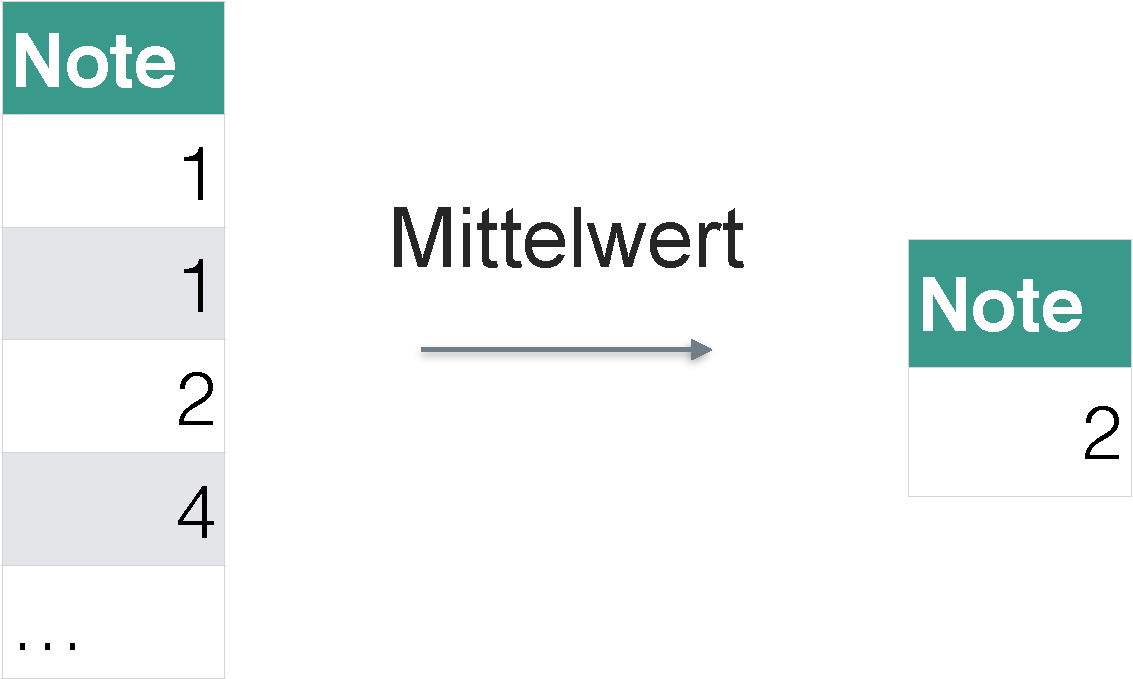
\includegraphics[width=0.7\linewidth]{images/summarise} 

}

\caption{Spalten zu einer Zahl zusammenfassen}\label{fig:fig-summarise}
\end{figure}

\begin{Shaded}
\begin{Highlighting}[]
\KeywordTok{summarise}\NormalTok{(stats_test, }\KeywordTok{mean}\NormalTok{(score))}
\CommentTok{#>   mean(score)}
\CommentTok{#> 1        31.1}
\end{Highlighting}
\end{Shaded}

Man könnte diesen Befehl so ins Deutsche übersetzen:
\texttt{Fasse\ aus\ Tabelle\ stats\_test\ die\ Spalte\ score\ anhand\ des\ Mittelwerts\ zusammen}.
Nicht vergessen, wenn die Spalte \texttt{score} fehlende Werte hat, wird
der Befehl \texttt{mean} standardmäßig dies mit \texttt{NA} quittieren.

Jetzt können wir auch die Gruppierung nutzen:

\begin{Shaded}
\begin{Highlighting}[]
\NormalTok{test_gruppiert <-}\StringTok{ }\KeywordTok{group_by}\NormalTok{(stats_test, interest)}
\KeywordTok{summarise}\NormalTok{(test_gruppiert, }\KeywordTok{mean}\NormalTok{(score))}
\CommentTok{#> # A tibble: 7 × 2}
\CommentTok{#>   interest `mean(score)`}
\CommentTok{#>      <int>         <dbl>}
\CommentTok{#> 1        1          28.3}
\CommentTok{#> 2        2          29.7}
\CommentTok{#> 3        3          30.8}
\CommentTok{#> 4        4          29.9}
\CommentTok{#> 5        5          32.5}
\CommentTok{#> 6        6          34.0}
\CommentTok{#> 7       NA          33.1}
\end{Highlighting}
\end{Shaded}

Der Befehl \texttt{summarise} erkennt also, wenn eine (mit
\texttt{group\_by}) gruppierte Tabelle vorliegt. Jegliche
Zusammenfassung, die wir anfordern, wird anhand der
Gruppierungsinformation aufgeteilt werden. In dem Beispiel bekommen wir
einen Mittelwert für jeden Wert von \texttt{interest}.
Interessanterweise sehen wir, dass der Mittelwert tendenziell größer
wird, je größer \texttt{interest} wird.

Alle diese \texttt{dplyr}-Befehle geben einen Dataframe zurück, was
praktisch ist für weitere Verarbeitung. In diesem Fall heißen die
Spalten \texttt{interst} und \texttt{mean(score)}. Zweiter Name ist
nicht so schön, daher ändern wir den wie folgt:

Jetzt können wir auch die Gruppierung nutzen:

\begin{Shaded}
\begin{Highlighting}[]
\NormalTok{test_gruppiert <-}\StringTok{ }\KeywordTok{group_by}\NormalTok{(stats_test, interest)}
\KeywordTok{summarise}\NormalTok{(test_gruppiert, }\DataTypeTok{mw_pro_gruppe =} \KeywordTok{mean}\NormalTok{(score, }\DataTypeTok{na.rm =} \OtherTok{TRUE}\NormalTok{))}
\CommentTok{#> # A tibble: 7 × 2}
\CommentTok{#>   interest mw_pro_gruppe}
\CommentTok{#>      <int>         <dbl>}
\CommentTok{#> 1        1          28.3}
\CommentTok{#> 2        2          29.7}
\CommentTok{#> 3        3          30.8}
\CommentTok{#> 4        4          29.9}
\CommentTok{#> 5        5          32.5}
\CommentTok{#> 6        6          34.0}
\CommentTok{#> 7       NA          33.1}
\end{Highlighting}
\end{Shaded}

Nun heißt die zweite Spalte \texttt{mw\_pro\_Gruppe}.
\texttt{na.rm\ =\ TRUE} veranlasst, bei fehlenden Werten trotzdem einen
Mittelwert zurückzuliefern (die Zeilen mit fehlenden Werten werden in
dem Fall ignoriert).

Grundsätzlich ist die Philosophie der \texttt{dplyr}-Befehle: ``Mach nur
eine Sache, aber die dafür gut''. Entsprechend kann \texttt{summarise}
nur \emph{Spalten} zusammenfassen, aber keine \emph{Zeilen}.

Merke:

\begin{quote}
Mit summarise kann man eine Spalte eines Dataframes zu einem Wert
zusammenfassen.
\end{quote}

\subsection{\texorpdfstring{Zeilen zählen mit \texttt{n} und
\texttt{count}}{Zeilen zählen mit n und count}}\label{zeilen-zahlen-mit-n-und-count}

Ebenfalls nützlich ist es, Zeilen zu zählen. Im Gegensatz zum
Standardbefehle \texttt{nrow} versteht der \texttt{dyplr}-Befehl
\texttt{n}auch Gruppierungen. \texttt{n} darf nur innerhalb von
\texttt{summarise} oder ähnlichen \texttt{dplyr}-Befehlen verwendet
werden.

\begin{Shaded}
\begin{Highlighting}[]
\KeywordTok{summarise}\NormalTok{(stats_test, }\KeywordTok{n}\NormalTok{())}
\CommentTok{#>   n()}
\CommentTok{#> 1 306}
\KeywordTok{summarise}\NormalTok{(test_gruppiert, }\KeywordTok{n}\NormalTok{())}
\CommentTok{#> # A tibble: 7 × 2}
\CommentTok{#>   interest `n()`}
\CommentTok{#>      <int> <int>}
\CommentTok{#> 1        1    30}
\CommentTok{#> 2        2    47}
\CommentTok{#> 3        3    66}
\CommentTok{#> 4        4    41}
\CommentTok{#> 5        5    45}
\CommentTok{#> 6        6     9}
\CommentTok{#> 7       NA    68}
\KeywordTok{nrow}\NormalTok{(stats_test)}
\CommentTok{#> [1] 306}
\end{Highlighting}
\end{Shaded}

Außerhalb von gruppierten Datensätzen ist \texttt{nrow} meist
praktischer.

Praktischer ist der Befehl \texttt{count}, der nichts anderes ist als
die Hintereinanderschaltung von \texttt{group\_by} und \texttt{n}. Mit
\texttt{count} zählen wir die Häufigkeiten nach Gruppen; Gruppen sind
hier zumeist die Werte einer auszuzählenden Variablen (oder mehrerer
auszuzählender Variablen). Das macht \texttt{count} zu einem wichtigen
Helfer bei der Analyse von Häufigkeitsdaten.

\begin{Shaded}
\begin{Highlighting}[]
\NormalTok{dplyr::}\KeywordTok{count}\NormalTok{(stats_test, interest)}
\CommentTok{#> # A tibble: 7 × 2}
\CommentTok{#>   interest     n}
\CommentTok{#>      <int> <int>}
\CommentTok{#> 1        1    30}
\CommentTok{#> 2        2    47}
\CommentTok{#> 3        3    66}
\CommentTok{#> 4        4    41}
\CommentTok{#> 5        5    45}
\CommentTok{#> 6        6     9}
\CommentTok{#> 7       NA    68}
\NormalTok{dplyr::}\KeywordTok{count}\NormalTok{(stats_test, study_time)}
\CommentTok{#> # A tibble: 6 × 2}
\CommentTok{#>   study_time     n}
\CommentTok{#>        <int> <int>}
\CommentTok{#> 1          1    31}
\CommentTok{#> 2          2    49}
\CommentTok{#> 3          3    85}
\CommentTok{#> 4          4    56}
\CommentTok{#> 5          5    17}
\CommentTok{#> 6         NA    68}
\NormalTok{dplyr::}\KeywordTok{count}\NormalTok{(stats_test, interest, study_time)}
\CommentTok{#> Source: local data frame [29 x 3]}
\CommentTok{#> Groups: interest [?]}
\CommentTok{#> }
\CommentTok{#>    interest study_time     n}
\CommentTok{#>       <int>      <int> <int>}
\CommentTok{#> 1         1          1    12}
\CommentTok{#> 2         1          2     7}
\CommentTok{#> 3         1          3     8}
\CommentTok{#> 4         1          4     2}
\CommentTok{#> 5         1          5     1}
\CommentTok{#> 6         2          1     9}
\CommentTok{#> 7         2          2    15}
\CommentTok{#> 8         2          3    16}
\CommentTok{#> 9         2          4     6}
\CommentTok{#> 10        2          5     1}
\CommentTok{#> # ... with 19 more rows}
\end{Highlighting}
\end{Shaded}

Allgemeiner formuliert lautet die Syntax:
\texttt{count(df,\ Spalte1,\ ...)}, wobei \texttt{df} der Dataframe ist
und \texttt{Spalte1} die erste (es können mehrere sein) auszuzählende
Spalte. Gibt man z.B. zwei Spalten an, so wird pro Wert der 1. Spalte
die Häufigkeiten der 2. Spalte ausgegeben.

Merke:

\begin{quote}
n und count zählen die Anzahl der Zeilen, d.h. die Anzahl der Fälle.
\end{quote}

\subsection{Die Pfeife}\label{die-pfeife}

Die zweite Idee kann man salopp als ``Durchpfeifen'' bezeichnen;
ikonographisch mit diesem Symbol dargestellt
\texttt{\%\textgreater{}\%}\footnote{Eine Art Smiley für Nerds.}. Der
Begriff ``Durchpfeifen'' ist frei vom Englischen ``to pipe'' übernommen.
Hierbei ist gemeint, einen Datensatz sozusagen auf ein Fließband zu
legen und an jedem Arbeitsplatz einen Arbeitsschritt auszuführen. Der
springende Punkt ist, dass ein Dataframe als ``Rohstoff'' eingegeben
wird und jeder Arbeitsschritt seinerseits wieder einen Datafram
ausgiebt. Damit kann man sehr schön, einen ``Flow'' an Verarbeitung
erreichen, außerdem spart man sich Tipparbeit und die Syntax wird
lesbarer. Damit das Durchpfeifen funktioniert, benötigt man Befehle, die
als Eingabe einen Dataframe erwarten und wieder einen Dataframe
zurückliefern. Das Schaubild verdeutlich beispielhaft eine Abfolge des
Durchpfeifens.

\begin{figure}

{\centering 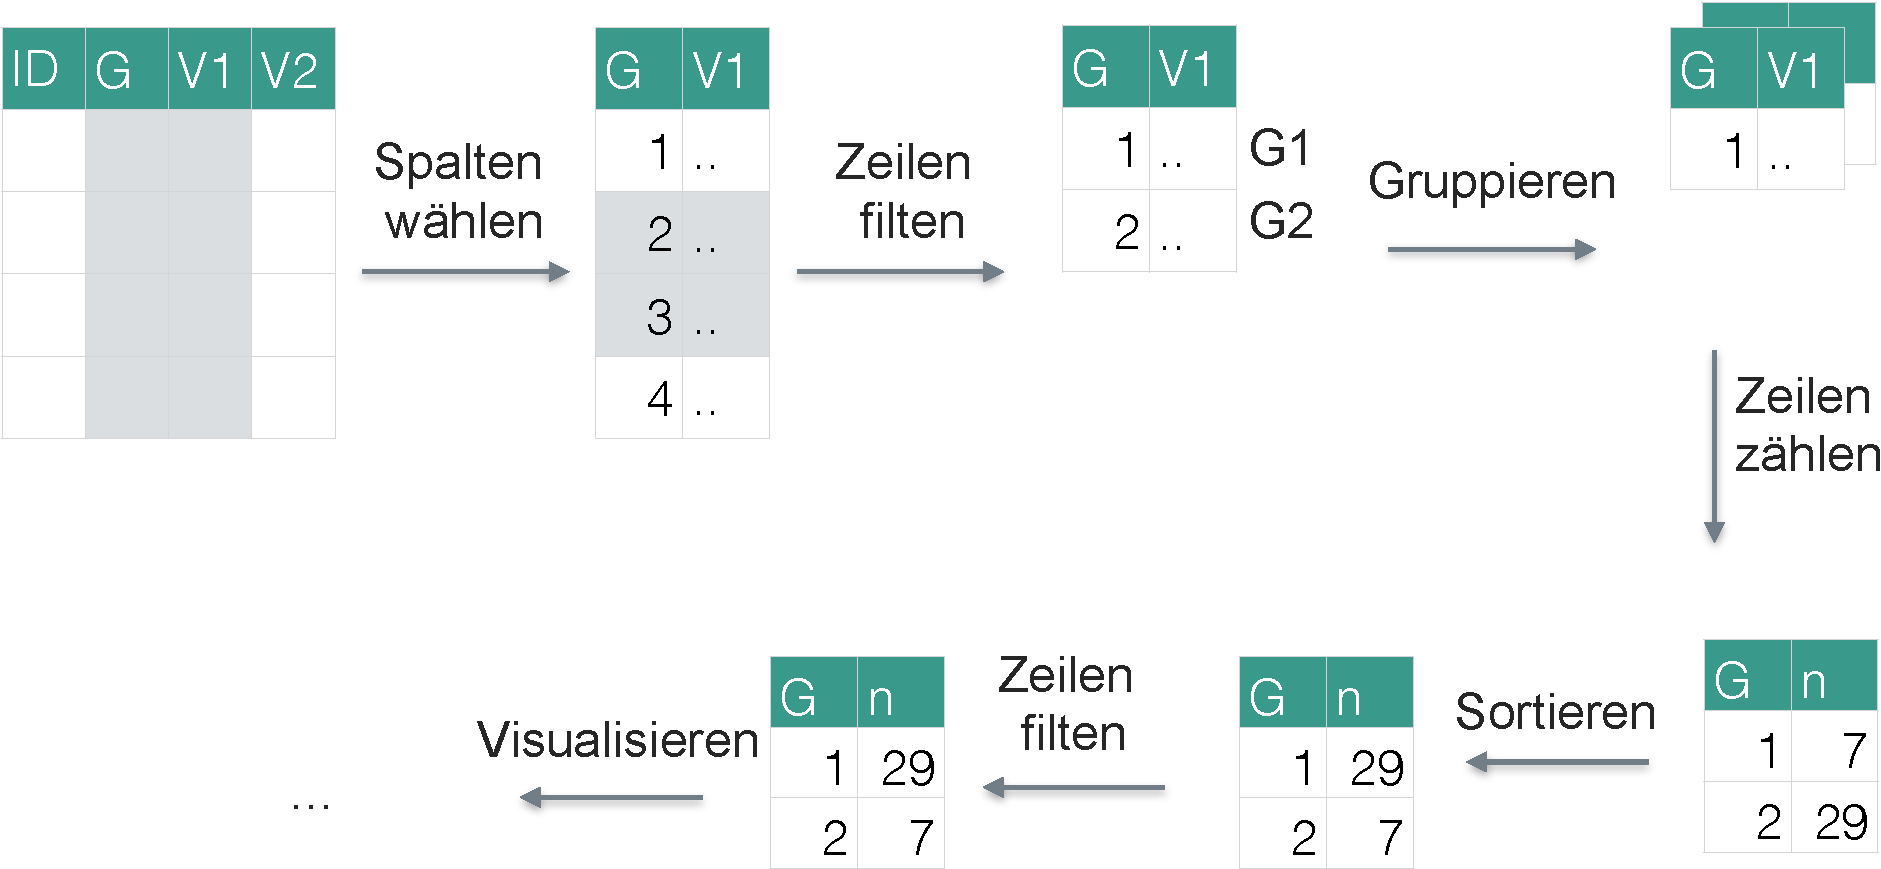
\includegraphics[width=0.8\linewidth]{images/durchpfeifen} 

}

\caption{Das 'Durchpeifen'}\label{fig:fig-durchpreifen}
\end{figure}

Die sog. ``Pfeife'' (pipe: \texttt{\%\textgreater{}\%}) in Anspielung an
das berühmte Bild von René Magritte, verkettet Befehle hintereinander.
Das ist praktisch, da es die Syntax vereinfacht. Vergleichen Sie mal
diese Syntax

\begin{Shaded}
\begin{Highlighting}[]
\KeywordTok{filter}\NormalTok{(}\KeywordTok{summarise}\NormalTok{(}\KeywordTok{group_by}\NormalTok{(}\KeywordTok{filter}\NormalTok{(stats_test, !}\KeywordTok{is.na}\NormalTok{(score)), interest), }\DataTypeTok{mw =} \KeywordTok{mean}\NormalTok{(score)), mw >}\StringTok{ }\DecValTok{30}\NormalTok{)}
\end{Highlighting}
\end{Shaded}

mit dieser

\begin{Shaded}
\begin{Highlighting}[]
\NormalTok{stats_test %>%}\StringTok{ }
\StringTok{  }\KeywordTok{filter}\NormalTok{(!}\KeywordTok{is.na}\NormalTok{(score)) %>%}\StringTok{ }
\StringTok{  }\KeywordTok{group_by}\NormalTok{(interest) %>%}\StringTok{ }
\StringTok{  }\KeywordTok{summarise}\NormalTok{(}\DataTypeTok{mw =} \KeywordTok{mean}\NormalTok{(score)) %>%}\StringTok{ }
\StringTok{  }\KeywordTok{filter}\NormalTok{(mw >}\StringTok{ }\DecValTok{30}\NormalTok{)}
\CommentTok{#> # A tibble: 4 × 2}
\CommentTok{#>   interest    mw}
\CommentTok{#>      <int> <dbl>}
\CommentTok{#> 1        3  30.8}
\CommentTok{#> 2        5  32.5}
\CommentTok{#> 3        6  34.0}
\CommentTok{#> 4       NA  33.1}
\end{Highlighting}
\end{Shaded}

Es ist hilfreich, diese ``Pfeifen-Syntax'' in deutschen Pseudo-Code zu
übersetzen.

\BeginKnitrBlock{rmdpseudocode}
Nimm die Tabelle ``stats\_test'' UND DANN\\
filtere alle nicht-fehlenden Werte UND DANN\\
gruppiere die verbleibenden Werte nach ``interest'' UND DANN\\
bilde den Mittelwert (pro Gruppe) für ``score'' UND DANN\\
liefere nur die Werte größer als 30 zurück.
\EndKnitrBlock{rmdpseudocode}

Die Pfeife zerlegt die ``russische Puppe'', also ineinander
verschachelteten Code, in sequenzielle Schritte und zwar in der
richtigen Reihenfolge (entsprechend der Abarbeitung). Wir müssen den
Code nicht mehr von innen nach außen lesen (wie das bei einer
mathematischen Formel der Fall ist), sondern können wie bei einem
Kochrezept ``erstens \ldots{}, zweitens .., drittens \ldots{}'' lesen.
Die Pfeife macht die Syntax einfacher. Natürlich hätten wir die
verschachtelte Syntax in viele einzelne Befehle zerlegen können und
jeweils eine Zwischenergebnis speichern mit dem Zuweisungspfeil
\texttt{\textless{}-} und das Zwischenergebnis dann explizit an den
nächsten Befehl weitergeben. Eigentlich macht die Pfeife genau das - nur
mit weniger Tipparbeit. Und auch einfacher zu lesen. Flow!

\subsection{\texorpdfstring{Werte umkodieren und
``binnen''}{Werte umkodieren und binnen}}\label{werte-umkodieren-und-binnen}

\subsubsection{\texorpdfstring{\texttt{car::recode}}{car::recode}}\label{carrecode}

Manchmal möchte man z.B. negativ gepolte Items umdrehen oder bei
kategoriellen Variablen kryptische Bezeichnungen in sprechendere
umwandeln (ein Klassiker ist \texttt{1} in \texttt{maennlich} bzw.
\texttt{2} in \texttt{weiblich} oder umgekehrt, kann sich niemand
merken). Hier gibt es eine Reihe praktischer Befehle, z.B.
\texttt{recode} aus dem Paket \texttt{car}. Übrigens: Wenn man explizit
angeben möchte, aus welchem Paket ein Befehl stammt (z.B. um
Verwechslungen zu vermeiden), gibt man \texttt{Paketnamen::Befehlnamen}
an. Schauen wir uns ein paar Beispiele zum Umkodieren an.

\begin{Shaded}
\begin{Highlighting}[]

\NormalTok{stats_test$score_fac <-}\StringTok{ }\NormalTok{car::}\KeywordTok{recode}\NormalTok{(stats_test$study_time, }\StringTok{"5 = 'sehr viel'; 2:4 = 'mittel'; 1 = 'wenig'"}\NormalTok{, }\DataTypeTok{as.factor.result =} \OtherTok{TRUE}\NormalTok{)}
\NormalTok{stats_test$score_fac <-}\StringTok{ }\NormalTok{car::}\KeywordTok{recode}\NormalTok{(stats_test$study_time, }\StringTok{"5 = 'sehr viel'; 2:4 = 'mittel'; 1 = 'wenig'"}\NormalTok{, }\DataTypeTok{as.factor.result =} \OtherTok{FALSE}\NormalTok{)}

\NormalTok{stats_test$study_time <-}\StringTok{ }\NormalTok{car::}\KeywordTok{recode}\NormalTok{(stats_test$study_time, }\StringTok{"5 = 'sehr viel'; 4 = 'wenig'; else = 'Hilfe'"}\NormalTok{, }\DataTypeTok{as.factor.result =} \OtherTok{TRUE}\NormalTok{)}

\KeywordTok{head}\NormalTok{(stats_test$study_time)}
\CommentTok{#> [1] sehr viel Hilfe     sehr viel Hilfe     wenig     Hilfe    }
\CommentTok{#> Levels: Hilfe sehr viel wenig}
\end{Highlighting}
\end{Shaded}

Der Befehle \texttt{recode} ist wirklich sehr prkatisch; mit \texttt{:}
kann man ``von bis'' ansprechen (das ginge mit \texttt{c()} übrigens
auch); \texttt{else} für ``ansonsten'' ist möglich und mit
\texttt{as.factor.result} kann man entweder einen Faktor oder eine
Text-Variable zurückgeliefert bekommen. Der ganze ``Wechselterm'' steht
in Anführungsstrichen (\texttt{"}). Einzelne Teile des Wechselterms sind
mit einem Strichpunkt (\texttt{;}) voneinander getrennt.

Das klassiche Umkodieren von Items aus Fragebögen kann man so anstellen;
sagen wir \texttt{interest} soll umkodiert werden:

\begin{Shaded}
\begin{Highlighting}[]
\NormalTok{stats_test$no_interest <-}\StringTok{ }\NormalTok{car::}\KeywordTok{recode}\NormalTok{(stats_test$interest, }\StringTok{"1 = 6; 2 = 5; 3 = 4; 4 = 3; 5 = 2; 6 = 1; else = NA"}\NormalTok{)}
\KeywordTok{glimpse}\NormalTok{(stats_test$no_interest)}
\CommentTok{#>  num [1:306] 2 4 1 5 1 NA NA 4 2 2 ...}
\end{Highlighting}
\end{Shaded}

Bei dem Wechselterm muss man aufpassen, nichts zu verwechseln; die
Zahlen sehen alle ähnlich aus\ldots{}

Testen kann man den Erfolg des Umpolens mit

\begin{Shaded}
\begin{Highlighting}[]
\NormalTok{dplyr::}\KeywordTok{count}\NormalTok{(stats_test, interest)}
\CommentTok{#> # A tibble: 7 × 2}
\CommentTok{#>   interest     n}
\CommentTok{#>      <int> <int>}
\CommentTok{#> 1        1    30}
\CommentTok{#> 2        2    47}
\CommentTok{#> 3        3    66}
\CommentTok{#> 4        4    41}
\CommentTok{#> 5        5    45}
\CommentTok{#> 6        6     9}
\CommentTok{#> 7       NA    68}
\NormalTok{dplyr::}\KeywordTok{count}\NormalTok{(stats_test, no_interest)}
\CommentTok{#> # A tibble: 7 × 2}
\CommentTok{#>   no_interest     n}
\CommentTok{#>         <dbl> <int>}
\CommentTok{#> 1           1     9}
\CommentTok{#> 2           2    45}
\CommentTok{#> 3           3    41}
\CommentTok{#> 4           4    66}
\CommentTok{#> 5           5    47}
\CommentTok{#> 6           6    30}
\CommentTok{#> 7          NA    68}
\end{Highlighting}
\end{Shaded}

Scheint zu passen. Noch praktischer ist, dass man so auch numerische
Variablen in Bereiche aufteilen kann (``binnen''):

\begin{Shaded}
\begin{Highlighting}[]
\NormalTok{stats_test$Ergebnis <-}\StringTok{ }\NormalTok{car::}\KeywordTok{recode}\NormalTok{(stats_test$score, }\StringTok{"1:38 = 'durchgefallen'; else = 'bestanden'"}\NormalTok{)}
\end{Highlighting}
\end{Shaded}

Natürlich gibt es auch eine Pfeifen komptatible Version, um Variablen
umzukodieren bzw. zu binnen: \texttt{dplyr::recode}\footnote{\url{https://blog.rstudio.org/2016/06/27/dplyr-0-5-0/}.}.
Die Syntax ist allerdings etwas weniger komfortabel (da strenger), so
dass wir an dieser Stelle bei \texttt{car::recode} bleiben.

\subsubsection{\texorpdfstring{Numerische Werte in Klassen gruppieren
mit
\texttt{cut}}{Numerische Werte in Klassen gruppieren mit cut}}\label{numerische-werte-in-klassen-gruppieren-mit-cut}

Numerische Werte in Klassen zu gruppieren (``to bin'', denglisch:
``binnen'') kann mit dem Befehl \texttt{cut} (and friends) besorgt
werden.

Es lassen sich drei typische Anwendungsformen unterscheiden:

Eine numerische Variable \ldots{}

\begin{enumerate}
\def\labelenumi{\arabic{enumi}.}
\tightlist
\item
  in \emph{k} gleich große Klassen grupieren (gleichgroße Intervalle)
\item
  so in Klassen gruppieren, dass in jeder Klasse \emph{n} Beobachtungen
  sind (gleiche Gruppengrößen)
\item
  in beliebige Klassen gruppieren
\end{enumerate}

\paragraph{gleichgroße Intervalle}\label{gleichgroe-intervalle}

Nehmen wir an, wir möchten die numerische Variable ``Körpergröße'' in
drei Gruppen einteilen: ``klein'', ``mittel'' und ``groß''. Der Range
von Körpergröße soll gleichmäßig auf die drei Gruppen aufgeteilt werden,
d.h. der Range (Interval) der drei Gruppen soll gleich groß sein. Dazu
kann man \texttt{cut\_interval} aus \texttt{ggplot2} nehmen {[}\^{}d.h.
\texttt{ggplot2} muss geladen sein; wenn man \texttt{tidyverse} lädt,
wird \texttt{ggplot2} automatisch auch geladen{]}.

\begin{Shaded}
\begin{Highlighting}[]
\NormalTok{wo_men <-}\StringTok{ }\KeywordTok{read_csv}\NormalTok{(}\StringTok{"data/wo_men.csv"}\NormalTok{)}

\NormalTok{wo_men %>%}\StringTok{ }
\StringTok{  }\KeywordTok{filter}\NormalTok{(height >}\StringTok{ }\DecValTok{150}\NormalTok{, height <}\StringTok{ }\DecValTok{220}\NormalTok{) ->}\StringTok{ }\NormalTok{wo_men2}

\NormalTok{temp <-}\StringTok{ }\KeywordTok{cut_interval}\NormalTok{(}\DataTypeTok{x =} \NormalTok{wo_men2$height, }\DataTypeTok{n =} \DecValTok{3}\NormalTok{)}

\KeywordTok{levels}\NormalTok{(temp)}
\CommentTok{#> [1] "[155,172]" "(172,189]" "(189,206]"}
\end{Highlighting}
\end{Shaded}

\texttt{cut\_interval} liefert eine Variabel vom Typ \texttt{factor}
zurück.

\paragraph{gleiche Gruppengrößen}\label{gleiche-gruppengroen}

\begin{Shaded}
\begin{Highlighting}[]
\NormalTok{temp <-}\StringTok{ }\KeywordTok{cut_number}\NormalTok{(wo_men2$height, }\DataTypeTok{n =} \DecValTok{2}\NormalTok{)}
\KeywordTok{str}\NormalTok{(temp)}
\CommentTok{#>  Factor w/ 2 levels "[155,169]","(169,206]": 1 2 2 2 2 1 1 2 1 2 ...}
\end{Highlighting}
\end{Shaded}

Mit \texttt{cut\_number} (aus ggplot2) kann man einen Vektor in
\texttt{n} Gruppen mit (etwa) gleich viel Observationen einteilen.

\begin{quote}
Teilt man einen Vektor in zwei gleich große Gruppen, so entspricht das
einer Aufteilung am Median (Median-Split).
\end{quote}

\subparagraph{In beliebige Klassen
gruppieren}\label{in-beliebige-klassen-gruppieren}

\begin{Shaded}
\begin{Highlighting}[]
\NormalTok{wo_men$groesse_gruppe <-}\StringTok{ }\KeywordTok{cut}\NormalTok{(wo_men$height, }
                             \DataTypeTok{breaks =} \KeywordTok{c}\NormalTok{(-}\OtherTok{Inf}\NormalTok{, }\DecValTok{100}\NormalTok{, }\DecValTok{150}\NormalTok{, }\DecValTok{170}\NormalTok{, }\DecValTok{200}\NormalTok{, }\DecValTok{230}\NormalTok{, }\OtherTok{Inf}\NormalTok{))}

\KeywordTok{count}\NormalTok{(wo_men, groesse_gruppe)}
\CommentTok{#> # A tibble: 6 × 2}
\CommentTok{#>   groesse_gruppe     n}
\CommentTok{#>           <fctr> <int>}
\CommentTok{#> 1     (-Inf,100]     4}
\CommentTok{#> 2      (150,170]    55}
\CommentTok{#> 3      (170,200]    38}
\CommentTok{#> 4      (200,230]     2}
\CommentTok{#> 5     (230, Inf]     1}
\CommentTok{#> 6             NA     1}
\end{Highlighting}
\end{Shaded}

\texttt{cut} ist im Standard-R (Paket ``base'') enthalten. Mit
\texttt{breaks} gibt man die Intervallgrenzen an. Zu beachten ist, dass
man eine Unter- bzw. Obergrenze angeben muss. D.h. der kleinste Wert
wird nicht automatisch als unterste Intervallgrenze herangezogen.

\section{\texorpdfstring{Fallstudie
\texttt{nycflights13}}{Fallstudie nycflights13}}\label{fallstudie-nycflights13}

Schauen wir uns einige Beispiele der Datenaufbereitung mittels
\texttt{dplyr} an. Wir verwenden hier den Datensatz \texttt{flights}aus
dem Package \texttt{nycflights13}. Der Datensatz ist recht groß
(\textasciitilde{}300.000 Zeilen und 19 Spalten); wenn man ihn als Excel
importiert, kann eine alte Möhre von Computer schon in die Knie gehen.
Beim Import als CSV habe ich noch nie von Problemen gehört; beim Import
via Package ebenfalls nicht. Werfen wir einen ersten Blick in die Daten:

\begin{Shaded}
\begin{Highlighting}[]
\KeywordTok{data}\NormalTok{(flights)}
\KeywordTok{glimpse}\NormalTok{(flights)}
\CommentTok{#> Observations: 336,776}
\CommentTok{#> Variables: 19}
\CommentTok{#> $ year           <int> 2013, 2013, 2013, 2013, 2013, 2013, 2013, 2013,...}
\CommentTok{#> $ month          <int> 1, 1, 1, 1, 1, 1, 1, 1, 1, 1, 1, 1, 1, 1, 1, 1,...}
\CommentTok{#> $ day            <int> 1, 1, 1, 1, 1, 1, 1, 1, 1, 1, 1, 1, 1, 1, 1, 1,...}
\CommentTok{#> $ dep_time       <int> 517, 533, 542, 544, 554, 554, 555, 557, 557, 55...}
\CommentTok{#> $ sched_dep_time <int> 515, 529, 540, 545, 600, 558, 600, 600, 600, 60...}
\CommentTok{#> $ dep_delay      <dbl> 2, 4, 2, -1, -6, -4, -5, -3, -3, -2, -2, -2, -2...}
\CommentTok{#> $ arr_time       <int> 830, 850, 923, 1004, 812, 740, 913, 709, 838, 7...}
\CommentTok{#> $ sched_arr_time <int> 819, 830, 850, 1022, 837, 728, 854, 723, 846, 7...}
\CommentTok{#> $ arr_delay      <dbl> 11, 20, 33, -18, -25, 12, 19, -14, -8, 8, -2, -...}
\CommentTok{#> $ carrier        <chr> "UA", "UA", "AA", "B6", "DL", "UA", "B6", "EV",...}
\CommentTok{#> $ flight         <int> 1545, 1714, 1141, 725, 461, 1696, 507, 5708, 79...}
\CommentTok{#> $ tailnum        <chr> "N14228", "N24211", "N619AA", "N804JB", "N668DN...}
\CommentTok{#> $ origin         <chr> "EWR", "LGA", "JFK", "JFK", "LGA", "EWR", "EWR"...}
\CommentTok{#> $ dest           <chr> "IAH", "IAH", "MIA", "BQN", "ATL", "ORD", "FLL"...}
\CommentTok{#> $ air_time       <dbl> 227, 227, 160, 183, 116, 150, 158, 53, 140, 138...}
\CommentTok{#> $ distance       <dbl> 1400, 1416, 1089, 1576, 762, 719, 1065, 229, 94...}
\CommentTok{#> $ hour           <dbl> 5, 5, 5, 5, 6, 5, 6, 6, 6, 6, 6, 6, 6, 6, 6, 5,...}
\CommentTok{#> $ minute         <dbl> 15, 29, 40, 45, 0, 58, 0, 0, 0, 0, 0, 0, 0, 0, ...}
\CommentTok{#> $ time_hour      <dttm> 2013-01-01 05:00:00, 2013-01-01 05:00:00, 2013...}
\end{Highlighting}
\end{Shaded}

Der Befehl \texttt{data} lädt Daten aus einem zuvor gestarteten Paket.

Achtung, Fallstudie. Sie sind der/die Assistent\_in des Chefs der New
Yorker Flughäfen. Ihr Chef kommt gut gelaunt ins Büro und sagt, dass er
diesen Schnarchnasen einheizen wolle und sagt, sie sollen ihm mal
schnell die Flüge mit der größten Verspätung raussuchen. Nix schickes,
aber zacki-zacki\ldots{}

\begin{Shaded}
\begin{Highlighting}[]
\NormalTok{flights %>%}\StringTok{ }
\StringTok{  }\KeywordTok{arrange}\NormalTok{(arr_delay)}
\CommentTok{#> # A tibble: 336,776 × 19}
\CommentTok{#>     year month   day dep_time sched_dep_time dep_delay arr_time}
\CommentTok{#>    <int> <int> <int>    <int>          <int>     <dbl>    <int>}
\CommentTok{#> 1   2013     5     7     1715           1729       -14     1944}
\CommentTok{#> 2   2013     5    20      719            735       -16      951}
\CommentTok{#> 3   2013     5     2     1947           1949        -2     2209}
\CommentTok{#> 4   2013     5     6     1826           1830        -4     2045}
\CommentTok{#> 5   2013     5     4     1816           1820        -4     2017}
\CommentTok{#> 6   2013     5     2     1926           1929        -3     2157}
\CommentTok{#> 7   2013     5     6     1753           1755        -2     2004}
\CommentTok{#> 8   2013     5     7     2054           2055        -1     2317}
\CommentTok{#> 9   2013     5    13      657            700        -3      908}
\CommentTok{#> 10  2013     1     4     1026           1030        -4     1305}
\CommentTok{#> # ... with 336,766 more rows, and 12 more variables: sched_arr_time <int>,}
\CommentTok{#> #   arr_delay <dbl>, carrier <chr>, flight <int>, tailnum <chr>,}
\CommentTok{#> #   origin <chr>, dest <chr>, air_time <dbl>, distance <dbl>, hour <dbl>,}
\CommentTok{#> #   minute <dbl>, time_hour <dttm>}
\end{Highlighting}
\end{Shaded}

Hm, übersichtlicher wäre es wahrscheinllich, wenn wir weniger Spalten
anschauen müssten. Am besten neben der Verspätung nur die Information,
die wir zur Identifizierung der Schuldigen\ldots{} will sagen der
gesuchten Flüge benötigen

\begin{Shaded}
\begin{Highlighting}[]
\NormalTok{flights %>%}\StringTok{ }
\StringTok{  }\KeywordTok{arrange}\NormalTok{(arr_delay) %>%}\StringTok{ }
\StringTok{  }\KeywordTok{select}\NormalTok{(arr_delay, carrier, month, day, dep_time, tailnum, flight, dest)}
\CommentTok{#> # A tibble: 336,776 × 8}
\CommentTok{#>    arr_delay carrier month   day dep_time tailnum flight  dest}
\CommentTok{#>        <dbl>   <chr> <int> <int>    <int>   <chr>  <int> <chr>}
\CommentTok{#> 1        -86      VX     5     7     1715  N843VA    193   SFO}
\CommentTok{#> 2        -79      VX     5    20      719  N840VA     11   SFO}
\CommentTok{#> 3        -75      UA     5     2     1947  N851UA    612   LAX}
\CommentTok{#> 4        -75      AA     5     6     1826  N3KCAA    269   SEA}
\CommentTok{#> 5        -74      AS     5     4     1816  N551AS      7   SEA}
\CommentTok{#> 6        -73      UA     5     2     1926  N24212   1628   SFO}
\CommentTok{#> 7        -71      DL     5     6     1753  N3760C   1394   PDX}
\CommentTok{#> 8        -71      UA     5     7     2054  N806UA    622   SFO}
\CommentTok{#> 9        -71      B6     5    13      657  N805JB    671   LAX}
\CommentTok{#> 10       -70      VX     1     4     1026  N855VA     23   SFO}
\CommentTok{#> # ... with 336,766 more rows}
\end{Highlighting}
\end{Shaded}

Da Zahlen in ihrer natürlichen Form von klein nach groß sortiert sind,
sortiert \texttt{arrange} in ebendieser Richtung. Wir können das
umdrehen mit einem Minuszeichen vor der zu sortierenden Spalte:

\begin{Shaded}
\begin{Highlighting}[]
\NormalTok{flights %>%}\StringTok{ }
\StringTok{  }\KeywordTok{arrange}\NormalTok{(-arr_delay) %>%}\StringTok{ }
\StringTok{  }\KeywordTok{select}\NormalTok{(arr_delay, carrier, month, day, dep_time, tailnum, flight, dest)}
\CommentTok{#> # A tibble: 336,776 × 8}
\CommentTok{#>    arr_delay carrier month   day dep_time tailnum flight  dest}
\CommentTok{#>        <dbl>   <chr> <int> <int>    <int>   <chr>  <int> <chr>}
\CommentTok{#> 1       1272      HA     1     9      641  N384HA     51   HNL}
\CommentTok{#> 2       1127      MQ     6    15     1432  N504MQ   3535   CMH}
\CommentTok{#> 3       1109      MQ     1    10     1121  N517MQ   3695   ORD}
\CommentTok{#> 4       1007      AA     9    20     1139  N338AA    177   SFO}
\CommentTok{#> 5        989      MQ     7    22      845  N665MQ   3075   CVG}
\CommentTok{#> 6        931      DL     4    10     1100  N959DL   2391   TPA}
\CommentTok{#> 7        915      DL     3    17     2321  N927DA   2119   MSP}
\CommentTok{#> 8        895      DL     7    22     2257  N6716C   2047   ATL}
\CommentTok{#> 9        878      AA    12     5      756  N5DMAA    172   MIA}
\CommentTok{#> 10       875      MQ     5     3     1133  N523MQ   3744   ORD}
\CommentTok{#> # ... with 336,766 more rows}
\end{Highlighting}
\end{Shaded}

Eine kleine Zugabe: Mit dem Befehl \texttt{knitr::kable} kann man einen
Dateframe automatisch in eine (einigermaßen) schöne Tabelle ausgeben
lassen. Oh halt, wir wollen keine Tabelle mit 300.000 Zeilen (der Chef
ist kein Freund von Details). Also begrenzen wir die Ausgabe auf die
ersten 10 Plätze.

\begin{Shaded}
\begin{Highlighting}[]
\NormalTok{flights %>%}\StringTok{ }
\StringTok{  }\KeywordTok{arrange}\NormalTok{(-arr_delay) %>%}\StringTok{ }
\StringTok{  }\KeywordTok{select}\NormalTok{(arr_delay, carrier, month, day, dep_time, tailnum, flight, dest) %>%}\StringTok{ }
\StringTok{  }\KeywordTok{filter}\NormalTok{(}\KeywordTok{row_number}\NormalTok{() <}\StringTok{ }\DecValTok{11}\NormalTok{) %>%}\StringTok{ }
\StringTok{  }\KeywordTok{kable}\NormalTok{()}
\end{Highlighting}
\end{Shaded}

\begin{tabular}{r|l|r|r|r|l|r|l}
\hline
arr\_delay & carrier & month & day & dep\_time & tailnum & flight & dest\\
\hline
1272 & HA & 1 & 9 & 641 & N384HA & 51 & HNL\\
\hline
1127 & MQ & 6 & 15 & 1432 & N504MQ & 3535 & CMH\\
\hline
1109 & MQ & 1 & 10 & 1121 & N517MQ & 3695 & ORD\\
\hline
1007 & AA & 9 & 20 & 1139 & N338AA & 177 & SFO\\
\hline
989 & MQ & 7 & 22 & 845 & N665MQ & 3075 & CVG\\
\hline
931 & DL & 4 & 10 & 1100 & N959DL & 2391 & TPA\\
\hline
915 & DL & 3 & 17 & 2321 & N927DA & 2119 & MSP\\
\hline
895 & DL & 7 & 22 & 2257 & N6716C & 2047 & ATL\\
\hline
878 & AA & 12 & 5 & 756 & N5DMAA & 172 & MIA\\
\hline
875 & MQ & 5 & 3 & 1133 & N523MQ & 3744 & ORD\\
\hline
\end{tabular}

``Geht doch'', war die Antwort des Chefs, als sie die Tabelle rübergeben
(er mag auch keine Emails). ``Ach ja'', raunt der Chef, als Sie das
Zimmer verlassen wollen, ``hatte ich erwähnt, dass ich die gleiche
Auswertung für jeden Carrier brauche? Reicht bis in einer halben
Stunde''.

Wir gruppieren also den Datensatz nach der Fluggesellschaft
(\texttt{carrier}) und filtern dann die ersten 3 Zeilen (damit die
Tabelle für den Chef nicht zu groß wird). Wie jeder
\texttt{dplyr}-Befehl wird die vorherige Gruppierung berücksichtigt und
daher die Top-3-Zeilen \emph{pro Gruppe}, d.h. pro Fluggesellschaft,
ausgegeben.

\begin{Shaded}
\begin{Highlighting}[]
\NormalTok{flights %>%}\StringTok{ }
\StringTok{  }\KeywordTok{arrange}\NormalTok{(-arr_delay) %>%}\StringTok{ }
\StringTok{  }\KeywordTok{select}\NormalTok{(arr_delay, carrier, month, day, dep_time, tailnum, flight, dest) %>%}\StringTok{ }
\StringTok{  }\KeywordTok{group_by}\NormalTok{(carrier) %>%}\StringTok{ }
\StringTok{  }\KeywordTok{filter}\NormalTok{(}\KeywordTok{row_number}\NormalTok{() <}\StringTok{ }\DecValTok{4}\NormalTok{) }
\CommentTok{#> Source: local data frame [48 x 8]}
\CommentTok{#> Groups: carrier [16]}
\CommentTok{#> }
\CommentTok{#>    arr_delay carrier month   day dep_time tailnum flight  dest}
\CommentTok{#>        <dbl>   <chr> <int> <int>    <int>   <chr>  <int> <chr>}
\CommentTok{#> 1       1272      HA     1     9      641  N384HA     51   HNL}
\CommentTok{#> 2       1127      MQ     6    15     1432  N504MQ   3535   CMH}
\CommentTok{#> 3       1109      MQ     1    10     1121  N517MQ   3695   ORD}
\CommentTok{#> 4       1007      AA     9    20     1139  N338AA    177   SFO}
\CommentTok{#> 5        989      MQ     7    22      845  N665MQ   3075   CVG}
\CommentTok{#> 6        931      DL     4    10     1100  N959DL   2391   TPA}
\CommentTok{#> 7        915      DL     3    17     2321  N927DA   2119   MSP}
\CommentTok{#> 8        895      DL     7    22     2257  N6716C   2047   ATL}
\CommentTok{#> 9        878      AA    12     5      756  N5DMAA    172   MIA}
\CommentTok{#> 10       852      AA     5    19      713  N3HEAA    257   LAS}
\CommentTok{#> # ... with 38 more rows}
\end{Highlighting}
\end{Shaded}

Vielleicht gefällt dem Chef diese Darstellung (sortiert nach
\texttt{carrier}) besser:

\begin{Shaded}
\begin{Highlighting}[]
\NormalTok{flights %>%}\StringTok{ }
\StringTok{  }\KeywordTok{arrange}\NormalTok{(-arr_delay) %>%}\StringTok{ }
\StringTok{  }\KeywordTok{select}\NormalTok{(arr_delay, carrier, month, day, dep_time, tailnum, flight, dest) %>%}\StringTok{ }
\StringTok{  }\KeywordTok{group_by}\NormalTok{(carrier) %>%}\StringTok{ }
\StringTok{  }\KeywordTok{filter}\NormalTok{(}\KeywordTok{row_number}\NormalTok{() <}\StringTok{ }\DecValTok{4}\NormalTok{) %>%}\StringTok{ }
\StringTok{  }\KeywordTok{arrange}\NormalTok{(carrier)}
\CommentTok{#> Source: local data frame [48 x 8]}
\CommentTok{#> Groups: carrier [16]}
\CommentTok{#> }
\CommentTok{#>    arr_delay carrier month   day dep_time tailnum flight  dest}
\CommentTok{#>        <dbl>   <chr> <int> <int>    <int>   <chr>  <int> <chr>}
\CommentTok{#> 1        744      9E     2    16      757  N8940E   3798   CLT}
\CommentTok{#> 2        458      9E     7    24     1525  N927XJ   3538   MSP}
\CommentTok{#> 3        421      9E     7    10     2054  N937XJ   3325   DFW}
\CommentTok{#> 4       1007      AA     9    20     1139  N338AA    177   SFO}
\CommentTok{#> 5        878      AA    12     5      756  N5DMAA    172   MIA}
\CommentTok{#> 6        852      AA     5    19      713  N3HEAA    257   LAS}
\CommentTok{#> 7        198      AS     3     8     1012  N587AS     11   SEA}
\CommentTok{#> 8        196      AS     1    20     2157  N305AS      7   SEA}
\CommentTok{#> 9        188      AS     5    23     2205  N516AS      7   SEA}
\CommentTok{#> 10       497      B6     1    16     1622  N661JB    517   MCO}
\CommentTok{#> # ... with 38 more rows}
\end{Highlighting}
\end{Shaded}

Da Sie den Chef gut kennen, berechnen Sie gleich noch die
durchschnittliche Verspätung pro Fluggesellschaft.

\begin{Shaded}
\begin{Highlighting}[]
\NormalTok{flights %>%}\StringTok{ }
\StringTok{  }\KeywordTok{select}\NormalTok{(arr_delay, carrier, month, day, dep_time, tailnum, flight, dest) %>%}\StringTok{ }
\StringTok{  }\KeywordTok{group_by}\NormalTok{(carrier) %>%}\StringTok{ }
\StringTok{  }\KeywordTok{summarise}\NormalTok{(}\DataTypeTok{delay_mean =} \KeywordTok{mean}\NormalTok{(arr_delay, }\DataTypeTok{na.rm =} \OtherTok{TRUE}\NormalTok{)) %>%}\StringTok{ }
\StringTok{  }\KeywordTok{arrange}\NormalTok{(-delay_mean) %>%}\StringTok{ }
\StringTok{  }\KeywordTok{kable}\NormalTok{()}
\end{Highlighting}
\end{Shaded}

\begin{tabular}{l|r}
\hline
carrier & delay\_mean\\
\hline
F9 & 21.921\\
\hline
FL & 20.116\\
\hline
EV & 15.796\\
\hline
YV & 15.557\\
\hline
OO & 11.931\\
\hline
MQ & 10.775\\
\hline
WN & 9.649\\
\hline
B6 & 9.458\\
\hline
9E & 7.380\\
\hline
UA & 3.558\\
\hline
US & 2.130\\
\hline
VX & 1.764\\
\hline
DL & 1.644\\
\hline
AA & 0.364\\
\hline
HA & -6.915\\
\hline
AS & -9.931\\
\hline
\end{tabular}

Der Chef ist zufrieden. Sie können sich wieder wichtigeren Aufgaben
zuwenden\ldots{}

\section{Checkliste zum Datenjudo}\label{checkliste-zum-datenjudo}

Fassen wir einige wesentliche Arbeitsschritte der Datenaufbereitung
zusammen{[}\^{}10{]}.

\subsection{Auf fehlende Werte prüfen*}\label{auf-fehlende-werte-prufen}

Das geht recht einfach mit \texttt{summarise(meine\_daten)}. Der Befehl
liefert für jede Spalte die Anzahl der fehlenden Werte zurück.

\begin{Shaded}
\begin{Highlighting}[]
\NormalTok{wo_men <-}\StringTok{ }\KeywordTok{read.csv}\NormalTok{(}\StringTok{"https://sebastiansauer.github.io/data/wo_men.csv"}\NormalTok{)}
\KeywordTok{summary}\NormalTok{(wo_men)}
\CommentTok{#>                   time       sex         height      shoe_size   }
\CommentTok{#>  11.10.2016 12:31:59: 2   man  :18   Min.   :  2   Min.   :35.0  }
\CommentTok{#>  11.10.2016 12:32:10: 2   woman:82   1st Qu.:163   1st Qu.:38.0  }
\CommentTok{#>  11.10.2016 12:32:32: 2   NA's : 1   Median :168   Median :39.0  }
\CommentTok{#>  11.10.2016 12:32:33: 2              Mean   :165   Mean   :39.8  }
\CommentTok{#>  11.10.2016 12:32:42: 2              3rd Qu.:174   3rd Qu.:40.0  }
\CommentTok{#>  04.10.2016 17:58:51: 1              Max.   :364   Max.   :88.0  }
\CommentTok{#>  (Other)            :90              NA's   :1     NA's   :1}
\end{Highlighting}
\end{Shaded}

\subsection{Fälle mit fehlenden Werte
löschen}\label{falle-mit-fehlenden-werte-loschen}

Weist eine Variable (Spalte) ``wenig'' fehlende Werte auf, so kann es
schlau sein, nichts zu tun. Eine andere Möglichkeit besteht darin, alle
entsprechenden Zeilen zu löschen. Man sollte aber schauen, wie viele
Zeilen dadurch verloren gehen.

\begin{Shaded}
\begin{Highlighting}[]
\KeywordTok{nrow}\NormalTok{(wo_men)}
\CommentTok{#> [1] 101}
\NormalTok{wo_men %>%}\StringTok{ }
\StringTok{  }\NormalTok{na.omit %>%}\StringTok{ }
\StringTok{  }\NormalTok{nrow}
\CommentTok{#> [1] 100}
\end{Highlighting}
\end{Shaded}

Hier verlieren wir nur 1 Zeile, das verschmerzen wir. Welche eigentlich?

\begin{Shaded}
\begin{Highlighting}[]
\NormalTok{wo_men %>%}\StringTok{ }
\StringTok{  }\NormalTok{rownames_to_column %>%}\StringTok{  }\CommentTok{# Zeilennummer werden eine eigene Spalte}
\StringTok{  }\KeywordTok{filter}\NormalTok{(!}\KeywordTok{complete.cases}\NormalTok{(.))  }\CommentTok{# Nur die nicht-kompletten Fälle filtern}
\CommentTok{#>   rowname                time  sex height shoe_size}
\CommentTok{#> 1      86 11.10.2016 12:44:06 <NA>     NA        NA}
\end{Highlighting}
\end{Shaded}

Man beachte, dass der Punkt \texttt{.} für den Datensatz steht, wie er
vom letzten Schritt weitergegeben wurde. Natürlich könnten wir diesen
Datensatz jetzt als neues Objekt speichern und damit weiter arbeiten.

\subsection{Fehlende Werte ggf.
ersetzen}\label{fehlende-werte-ggf.-ersetzen}

Ist die Anzahl der fehlenden Werte zu groß, als dass wir es verkraften
könnten, die Zeilen zu löschen, so können wir die fehlenden Werte
ersetzen. Allein, das ist ein weites Feld und übersteigt den Anspruch
dieses Kurses{[}\^{}Das sagen Autoren, wenn sie nicht genau wissen, wie
etwas funktioniert.{]}. Eine einfache, aber nicht die beste Möglichkeit,
besteht darin, die fehlenden Werte durch einen repräsentativen Wert,
z.B. den Mittelwert der Spalte, zu ersetzen.

\begin{Shaded}
\begin{Highlighting}[]
\NormalTok{wo_men$height <-}\StringTok{ }\KeywordTok{replace}\NormalTok{(wo_men$height, }\KeywordTok{is.na}\NormalTok{(wo_men$height), }\KeywordTok{mean}\NormalTok{(wo_men$height, }\DataTypeTok{na.rm =} \OtherTok{TRUE}\NormalTok{))}
  
\end{Highlighting}
\end{Shaded}

\texttt{replace} ersetzt Werte aus dem Vektor \texttt{wo\_men\$height}
alle Werte, für die \texttt{is.na(wo\_men\$height)} wahr ist. Diese
Werte werden durch den Mittelwert der Spalte ersetzt\footnote{Hier
  findet sich eine ausführliche Darstellung:
  \url{https://sebastiansauer.github.io/checklist_data_cleansing/index.html}}.

\subsection{Nach Fehlern suchen}\label{nach-fehlern-suchen}

Leicht schleichen sich Tippfehler oder andere Fehler ein. Man sollte
darauf prüfen; so könnte man sich ein Histogramm ausgeben lassen pro
Variable, um ``ungewöhnliche'' Werte gut zu erkennen. Meist geht das
besser als durch das reine Betrachten von Zahlen. Gibt es wenig
unterschiedliche Werte, so kann man sich auch die unterschiedlichen
Werte ausgeben lassen.

\begin{Shaded}
\begin{Highlighting}[]
\NormalTok{wo_men %>%}\StringTok{ }
\StringTok{  }\KeywordTok{count}\NormalTok{(shoe_size) %>%}\StringTok{ }
\StringTok{  }\NormalTok{head  }\CommentTok{# nur die ersten paar Zeilen}
\CommentTok{#> # A tibble: 6 × 2}
\CommentTok{#>   shoe_size     n}
\CommentTok{#>       <dbl> <int>}
\CommentTok{#> 1      35.0     1}
\CommentTok{#> 2      36.0     6}
\CommentTok{#> 3      36.5     1}
\CommentTok{#> 4      37.0    14}
\CommentTok{#> 5      38.0    26}
\CommentTok{#> 6      39.0    18}
\end{Highlighting}
\end{Shaded}

\subsection{Ausreiser identifizieren}\label{ausreiser-identifizieren}

Ähnlich zu Fehlern, steht man Ausreisern häufig skeptisch gegenüber.
Allerdings kann man nicht pauschal sagen, das Extremwerte entfernt
werden sollen: Vielleicht war jemand in der Stichprobe wirklich nur
1.20m groß? Hier gilt es, begründet und nachvollziehbar im Einzelfall zu
entscheiden. Histogramme und Boxplots sind wieder ein geeignetes Mittel,
um Ausreiser zu finden.

\subsection{Hochkorrelierte Variablen
finden}\label{hochkorrelierte-variablen-finden}

Haben zwei Leute die gleiche Meinung, so ist einer von beiden
überflüssig - wird behauptet. Ähnlich bei Variablen; sind zwei Variablen
sehr hoch korreliert (\textgreater{}.9, als grober (!) Richtwert), so
bringt die zweite kaum Informationszuwachs zur ersten. Und kann
ausgeschlossen werden. Oder man fasst ähnliche Variablen zusammen.

\begin{Shaded}
\begin{Highlighting}[]
\NormalTok{wo_men %>%}\StringTok{ }
\StringTok{  }\KeywordTok{select}\NormalTok{(height, shoe_size) %>%}\StringTok{ }
\StringTok{  }\KeywordTok{correlate}\NormalTok{() ->}\StringTok{ }\NormalTok{km   }\CommentTok{# Korrelationsmatrix berechnen}
\NormalTok{km  }
\CommentTok{#> # A tibble: 2 × 3}
\CommentTok{#>     rowname height shoe_size}
\CommentTok{#>       <chr>  <dbl>     <dbl>}
\CommentTok{#> 1    height     NA     0.553}
\CommentTok{#> 2 shoe_size  0.553        NA}

\NormalTok{km %>%}\StringTok{ }
\StringTok{  }\KeywordTok{shave}\NormalTok{() %>%}\StringTok{ }\CommentTok{# Oberes Dreieck ist redundant, wird "abrasiert"}
\StringTok{  }\KeywordTok{rplot}\NormalTok{()  }\CommentTok{# Korrelationsplot}
\end{Highlighting}
\end{Shaded}

\begin{center}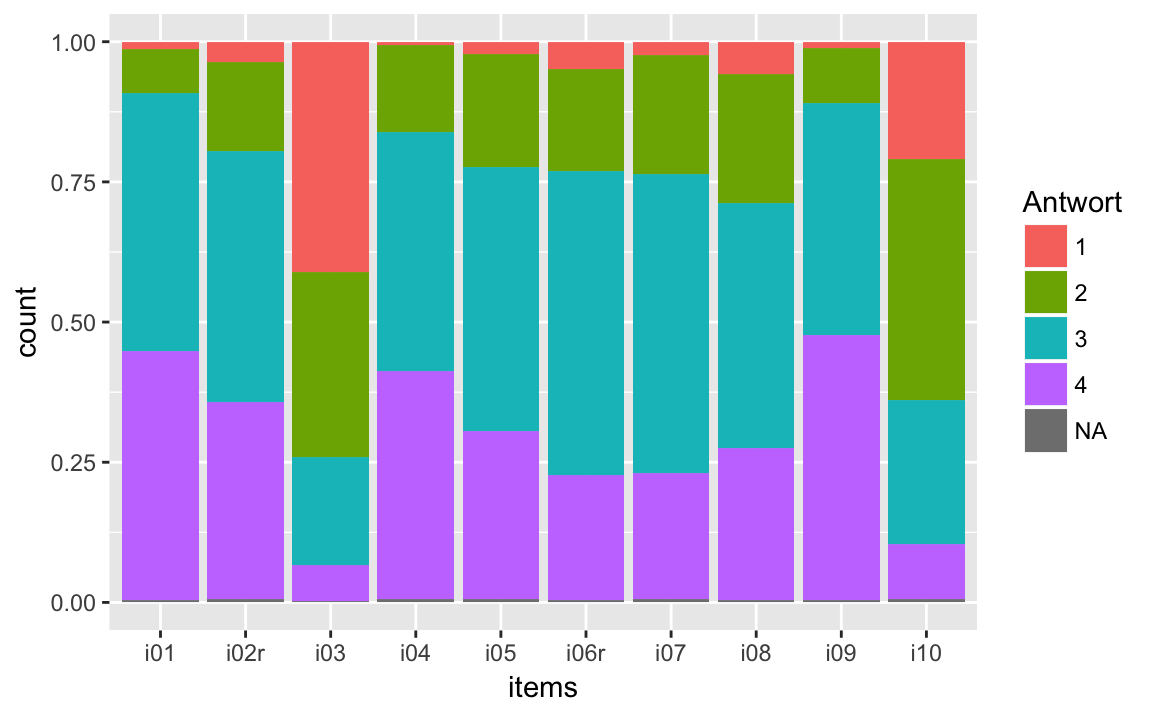
\includegraphics[width=0.7\linewidth]{040_Datenjudo_files/figure-latex/unnamed-chunk-38-1} \end{center}

Die Funktion \texttt{correlate} stammt aus dem Paket
\texttt{corrr}\footnote{\url{https://github.com/drsimonj/corrr}},
welches vorher installiert und geladen sein muss. Hier ist die
Korrelation nicht zu groß, so dass wir keine weiteren Schritte
unternehmen.

\subsection{z-Standardisieren}\label{z-standardisieren}

Für eine Reihe von Analysen ist es wichtig, die Skalierung der Variablen
zur vereinheitlichen. Die z-Standardisierung ist ein übliches Vorgehen.
Dabei wird der Mittelwert auf 0 transformiert und die SD auf 1; man
spricht - im Falle von (hinreichend) normalverteilten Variablen - jetzt
von der \emph{Standardnormalverteilung}\index{Standardnormalverteilung}.
Unterscheiden sich zwei Objekte A und B in einer
standardnormalverteilten Variablen, so sagt dies nur etwas zur relativen
Position von A zu B innerhalb ihrer Verteilung aus - im Gegensatz zu den
Rohwerten.

\begin{Shaded}
\begin{Highlighting}[]
\NormalTok{wo_men %>%}\StringTok{ }
\StringTok{  }\KeywordTok{select_if}\NormalTok{(is.numeric) %>%}\StringTok{  }\CommentTok{# Spalte nur auswählen, wenn numerisch}
\StringTok{  }\KeywordTok{scale}\NormalTok{() %>%}\StringTok{  }\CommentTok{# z-standardisieren}
\StringTok{  }\KeywordTok{head}\NormalTok{()  }\CommentTok{# nur die ersten paar Zeilen abdrucken}
\CommentTok{#>      height shoe_size}
\CommentTok{#> [1,] -0.132    0.0405}
\CommentTok{#> [2,]  0.146   -0.1395}
\CommentTok{#> [3,]  0.221   -0.1395}
\CommentTok{#> [4,]  0.272    0.0405}
\CommentTok{#> [5,]  0.751    1.1204}
\CommentTok{#> [6,] -0.208   -0.4994}
\end{Highlighting}
\end{Shaded}

Dieser Befehl liefert zwei z-standardisierte Spalten zurück. Kommoder
ist es aber, alle Spalten des Datensatzes zurück zu bekommen, wobei
zusätzlich die z-Werte aller numerischen Variablen hinzugekommen sind:

\begin{Shaded}
\begin{Highlighting}[]
\NormalTok{wo_men %>%}\StringTok{ }
\StringTok{  }\KeywordTok{mutate_if}\NormalTok{(is.numeric, }\KeywordTok{funs}\NormalTok{(}\StringTok{"z"} \NormalTok{=}\StringTok{ }\NormalTok{scale)) %>%}\StringTok{ }
\StringTok{  }\NormalTok{head}
\CommentTok{#>                  time   sex height shoe_size height_z shoe_size_z}
\CommentTok{#> 1 04.10.2016 17:58:51 woman    160        40   -0.132      0.0405}
\CommentTok{#> 2 04.10.2016 17:58:59 woman    171        39    0.146     -0.1395}
\CommentTok{#> 3 04.10.2016 18:00:15 woman    174        39    0.221     -0.1395}
\CommentTok{#> 4 04.10.2016 18:01:17 woman    176        40    0.272      0.0405}
\CommentTok{#> 5 04.10.2016 18:01:22   man    195        46    0.751      1.1204}
\CommentTok{#> 6 04.10.2016 18:01:53 woman    157        37   -0.208     -0.4994}
\end{Highlighting}
\end{Shaded}

Der Befehl \texttt{mutate} berechnet eine neue Spalte;
\texttt{mutate\_if} tut dies, wenn die Spalte numerisch ist. Die neue
Spalte wird berechnet als z-Transformierung der alten Spalte; zum
Spaltenname wird ein ``\_z" hinzugefügt. Natürlich hätten wir auch mit
\texttt{select} ``händisch'' die relevanten Spalten auswählen können.

\subsection{Quasi-Konstante finden}\label{quasi-konstante-finden}

Hat eine Variable nur einen Wert, so verdient sie die Ehrenbezeichnung
``Variable'' nicht wirklich. Haben wir z.B. nur Männer im Datensatz, so
kann das Geschlecht nicht für Unterschiede im Einkommen verantwortlich
sein. Besser die Variable Geschlecht dann zu entfernen. Auch hier sind
Histogramme oder Boxplots von Nutzen zur Identifiktion von
(Quasi-)Konstanten. Alternativ kann man sich auch pro die Streuung
(numerische Variablen) oder die Anzahl unterschiedlicher Werte
(qualitative Variablen) ausgeben lassen.

\subsection{Auf Normalverteilung
prüfen}\label{auf-normalverteilung-prufen}

Einige statistische Verfahren gehen von normalverteilten Variablen aus,
daher macht es Sinn, Normalverteilung zu prüfen. \emph{Perfekte}
Normalverteilung ist genau so häufig, wie \emph{perfekte} Kreise in der
Natur. Entsprechend werden Signifikanztests, die ja auf perfekte
Normalverteilung prüfen, immer signifikant sein, sofern die Stichrprobe
groß genug ist. Daher ist meist zweckmäßiger, einen graphischen ``Test''
durchzuführen: Histogramm oder eine Dichte-Diagramm als ``glatt
geschmiergelte'' Variante des Histogramms bieten sich an.

\begin{Shaded}
\begin{Highlighting}[]
\NormalTok{wo_men %>%}\StringTok{ }
\StringTok{  }\KeywordTok{ggplot}\NormalTok{() +}
\StringTok{  }\KeywordTok{aes}\NormalTok{(}\DataTypeTok{x =} \NormalTok{height) +}
\StringTok{  }\KeywordTok{geom_density}\NormalTok{() ->}\StringTok{ }\NormalTok{p1}

\NormalTok{wo_men %>%}\StringTok{ }
\StringTok{  }\KeywordTok{ggplot}\NormalTok{() +}
\StringTok{  }\KeywordTok{aes}\NormalTok{(}\DataTypeTok{x =} \NormalTok{shoe_size) +}
\StringTok{  }\KeywordTok{geom_density}\NormalTok{() ->}\StringTok{ }\NormalTok{p2}

\KeywordTok{grid.arrange}\NormalTok{(p1, p2, }\DataTypeTok{ncol =} \DecValTok{2}\NormalTok{)}
\end{Highlighting}
\end{Shaded}

\begin{center}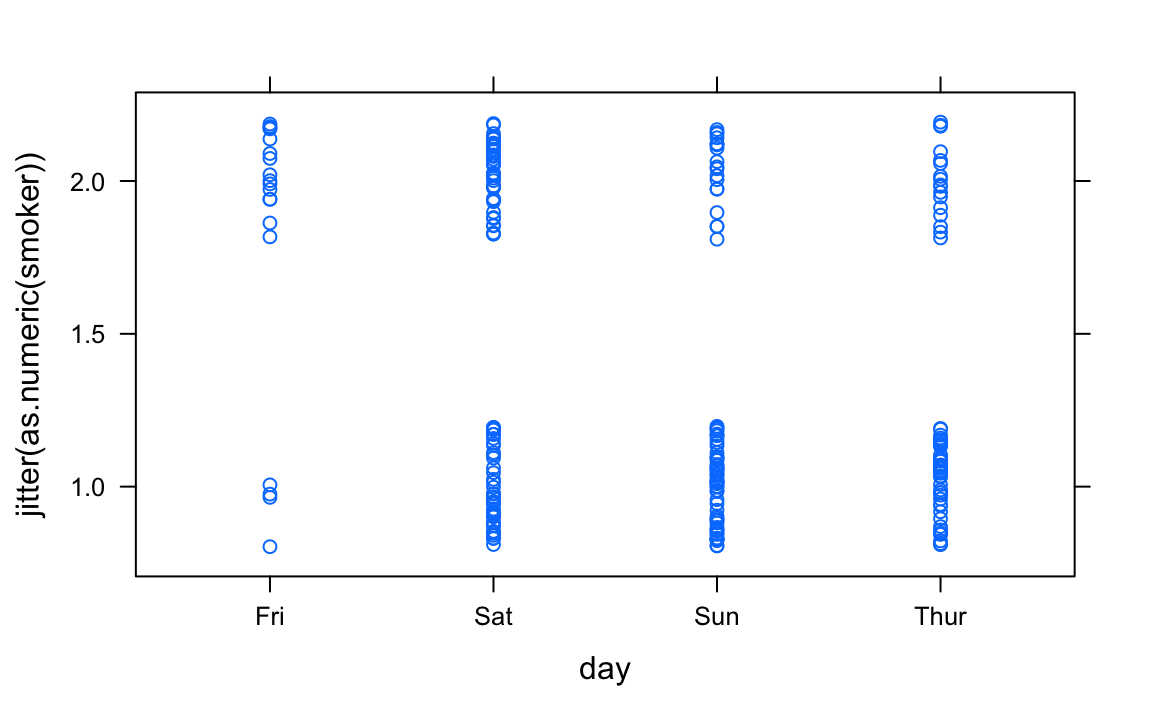
\includegraphics[width=0.7\linewidth]{040_Datenjudo_files/figure-latex/unnamed-chunk-41-1} \end{center}

Während die Körpergröße sehr deutlich normalverteilt ist, ist die
Schuhgröße recht schief. Bei schiefen Verteilung können Transformationen
Abhilfe schaffen. Hier erscheint die Schiefe noch erträglich, so dass
wir keine weiteren Maßnahmen einleiten.

\subsection{Mittelwerte pro Zeile
berechnen}\label{mittelwerte-pro-zeile-berechnen}

Um Umfragedaten auszuwerten, will man häufig einen Mittelwert \emph{pro
Zeile} berechnen. Normalerweise fasst man eine \emph{Spalte} zu einer
Zahl zusammen; aber jetzt, fassen wir eine \emph{Zeile} zu einer Zahl
zusammen. Der häufigste Fall ist, wie gesagt, einen Mittelwert zu bilden
für jede Person. Nehmen wir an, wir haben eine Befragung zur
Extraversion durchgeführt und möchten jetzt den mittleren
Extraversions-Wert pro Person (d.h. pro Zeile) berechnen.

\begin{Shaded}
\begin{Highlighting}[]
\NormalTok{extra <-}\StringTok{ }\KeywordTok{read.csv}\NormalTok{(}\StringTok{"data/extra.csv"}\NormalTok{)}

\NormalTok{extra_items <-}\StringTok{ }\NormalTok{extra %>%}\StringTok{ }
\StringTok{  }\KeywordTok{select}\NormalTok{(i01:i10)}

\NormalTok{extra$extra_mw <-}\StringTok{ }\KeywordTok{rowMeans}\NormalTok{(extra_items)}
\end{Highlighting}
\end{Shaded}

Da der Datensatz über 28 Spalten verfügt, wir aber nur 10 Spalten
heranziehen möchten, um Zeilen auf eine Zahl zusammenzufassen, bilden
wir als Zwischenschritt einen ``schmäleren'' Datensatz,
\texttt{extra\_items}. Im Anschluss berechnen wir mit \texttt{rowMeans}
die Mittelwerte pro Zeile (engl. ``row'').

\subsection{U}\label{u}

\begin{Shaded}
\begin{Highlighting}[]
\NormalTok{extra %>%}\StringTok{ }
\StringTok{  }\KeywordTok{count}\NormalTok{(n_faceb)}
\end{Highlighting}
\end{Shaded}

\section{Verweise}\label{verweise-2}

\begin{itemize}
\item
  Eine schöne Demonstration der Mächtigkeit von \texttt{dplyr} findet
  sich hier\footnote{\url{http://bit.ly/2kX9lvC}.}.
\item
  Die GUI ``exploratory'' ist ein ``klickbare'' Umsetzung von
  \texttt{dplyr}, mächtig, modern und sieht cool aus:
  \url{https://exploratory.io}.
\item
  \emph{R for Data Science} bietet umfangreiche Unterstützung zu diesem
  Thema (Wickham and Grolemund \protect\hyperlink{ref-r4ds}{2016}).
\end{itemize}

\chapter{Daten visualisieren}\label{daten-visualisieren}

Benötigte Pakete:

\begin{Shaded}
\begin{Highlighting}[]
\KeywordTok{library}\NormalTok{(tidyverse)  }\CommentTok{# Zum Plotten}
\KeywordTok{library}\NormalTok{(wesanderson)  }\CommentTok{# Farb-Palette von Wes Anderson}
\KeywordTok{library}\NormalTok{(car)  }\CommentTok{# Umkodieren}
\KeywordTok{library}\NormalTok{(RColorBrewer)  }\CommentTok{# Farb-Palette von Cynthia Breewr}
\KeywordTok{library}\NormalTok{(GGally)  }\CommentTok{# Scatterplot-Matrizen}
\KeywordTok{library}\NormalTok{(knitr)  }\CommentTok{# HTML-Tabellen}
\KeywordTok{library}\NormalTok{(gridExtra)  }\CommentTok{# Mehrere Plots in einem erstellen}
\KeywordTok{library}\NormalTok{(corrr)  }\CommentTok{# Korrelationsplots}
\end{Highlighting}
\end{Shaded}

\begin{center}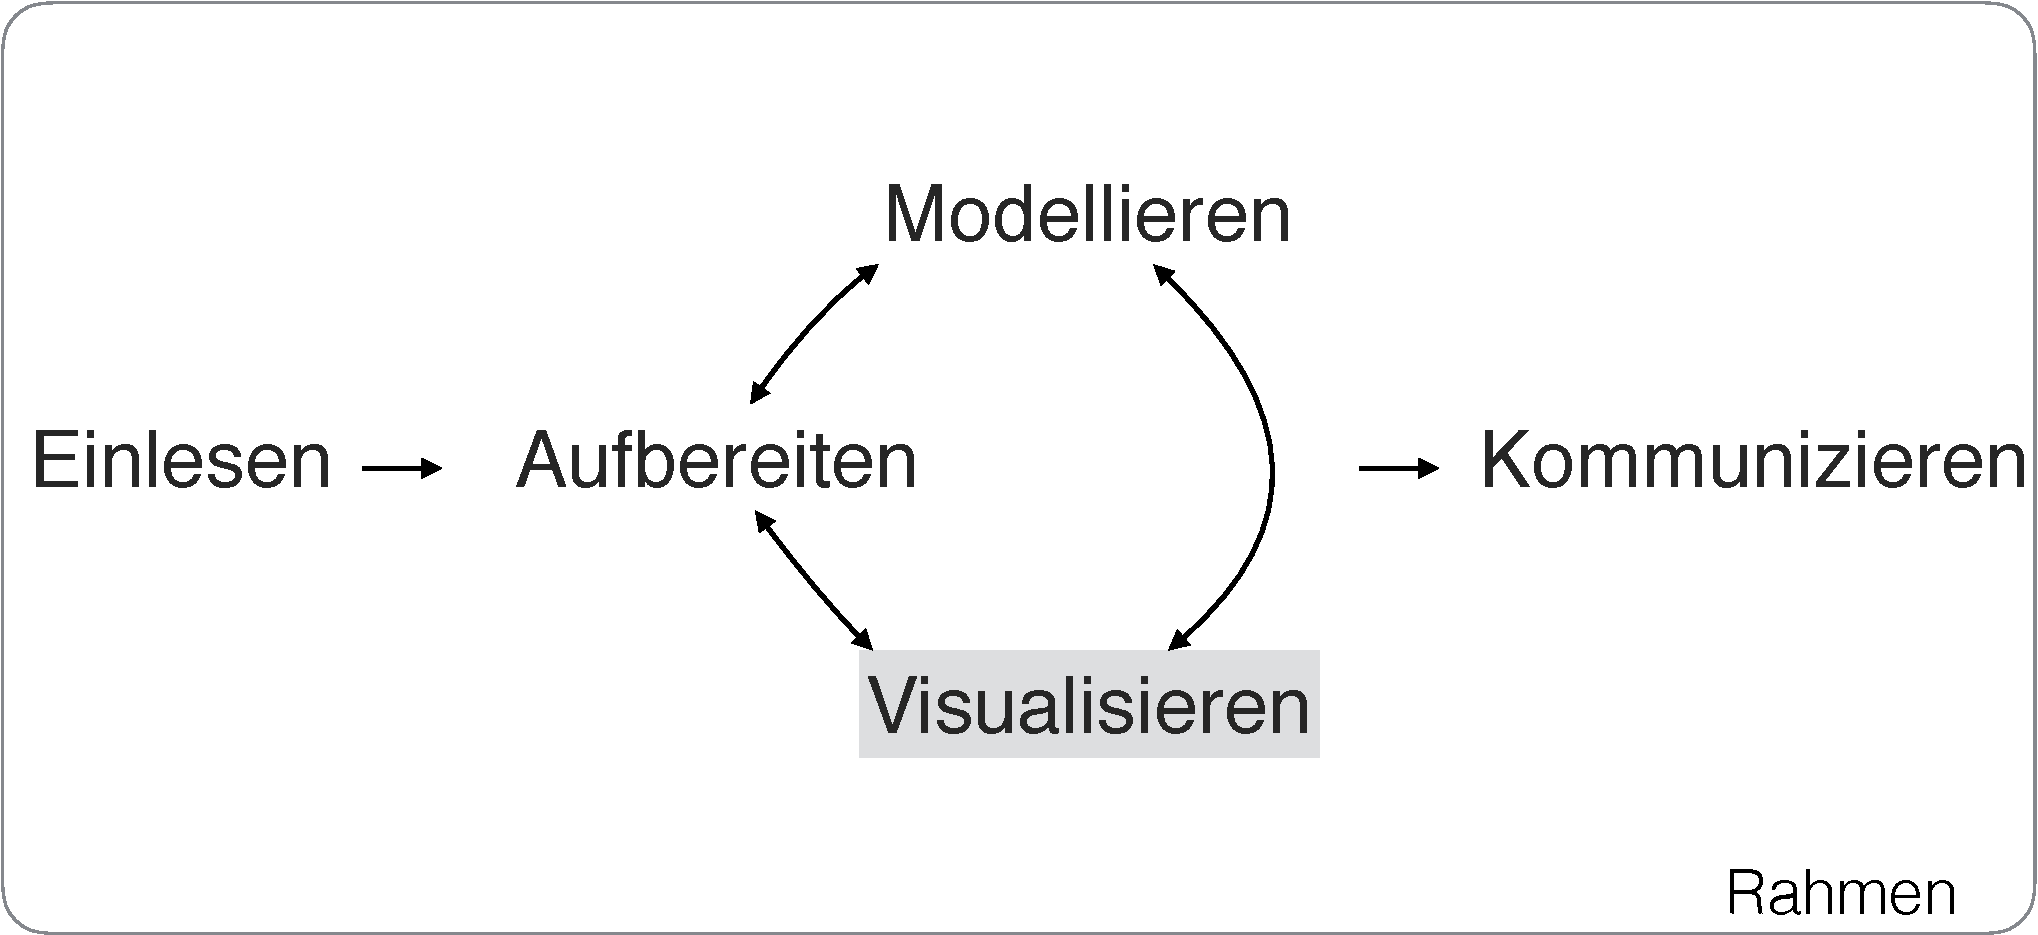
\includegraphics[width=0.7\linewidth]{images/Visualisieren} \end{center}

Ein Bild sagt bekanntlich mehr als 1000 Worte. Schauen wir uns zur
Verdeutlichung das berühmte Beispiel von
Anscombe{[}\^{}https://de.wikipedia.org/wiki/Anscombe-Quartett{]} an. Es
geht hier um vier Datensätze mit zwei Variablen (Spalten; X und Y).
Offenbar sind die Datensätze praktisch identisch: Alle X haben den
gleichen Mittelwert und die gleiche Varianz; dasselbe gilt für die Y.
Die Korrelation zwischen X und Y ist in allen vier Datensätzen gleich.
Allerdings erzählt eine Visualisierung der vier Datensätze eine ganz
andere Geschichte.

\begin{center}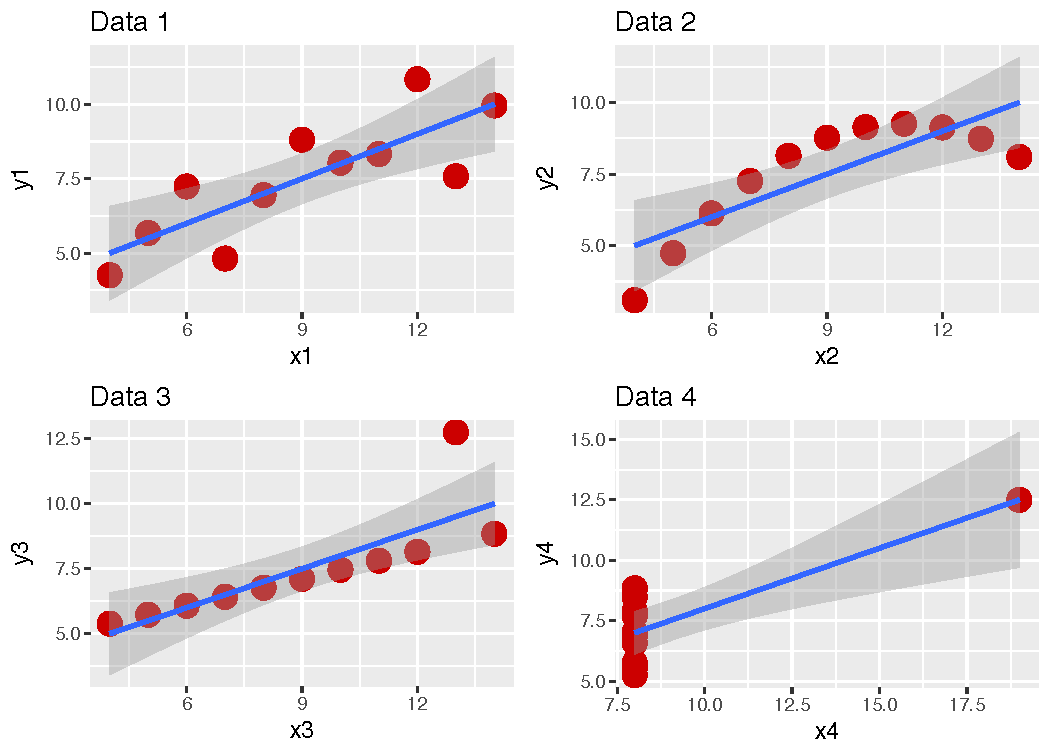
\includegraphics[width=0.7\linewidth]{images/anscombe} \end{center}

Offenbar ``passieren'' in den vier Datensätzen gänzlich unterschiedliche
Dinge. Dies haben die Statistiken nicht aufgedeckt; erst die
Visualisierung erhellte uns\ldots{} Kurz: Die Visualisierung ist ein
unverzichtbares Werkzeug, um zu verstehen, was in einem Datensatz (und
damit in der zugrundeliengenden ``Natur'') passiert.

Es gibt viele Möglichkeiten, Daten zu visualieren (in R). Wir werden uns
hier auf einen Weg bzw. ein Paket konzentrieren, der komfortabel, aber
mächtig ist und gut zum Prinzip des Durchpfeifens passt:
\texttt{ggplot2}{[}\^{}``gg'' steht für ``grammer of graphics'' nach
einem Buch von
Wilkinson(\protect\hyperlink{ref-wilkinson2006grammar}{2006}); ``plot''
steht für ``to plot'' also ein Diagramm erstellen (``plotten''); vgl.
\url{https://en.wikipedia.org/wiki/Ggplot2}{]}.

Laden wir dazu den Datensatz \texttt{nycflights::flights}.

\begin{Shaded}
\begin{Highlighting}[]
\KeywordTok{data}\NormalTok{(flights, }\DataTypeTok{package =} \StringTok{"nycflights13"}\NormalTok{)}
\end{Highlighting}
\end{Shaded}

\begin{Shaded}
\begin{Highlighting}[]
\KeywordTok{qplot}\NormalTok{(}\DataTypeTok{x =} \NormalTok{carrier, }\DataTypeTok{y =} \NormalTok{arr_delay, }\DataTypeTok{geom =} \StringTok{"boxplot"}\NormalTok{, }\DataTypeTok{data =} \NormalTok{flights)}
\end{Highlighting}
\end{Shaded}

\begin{center}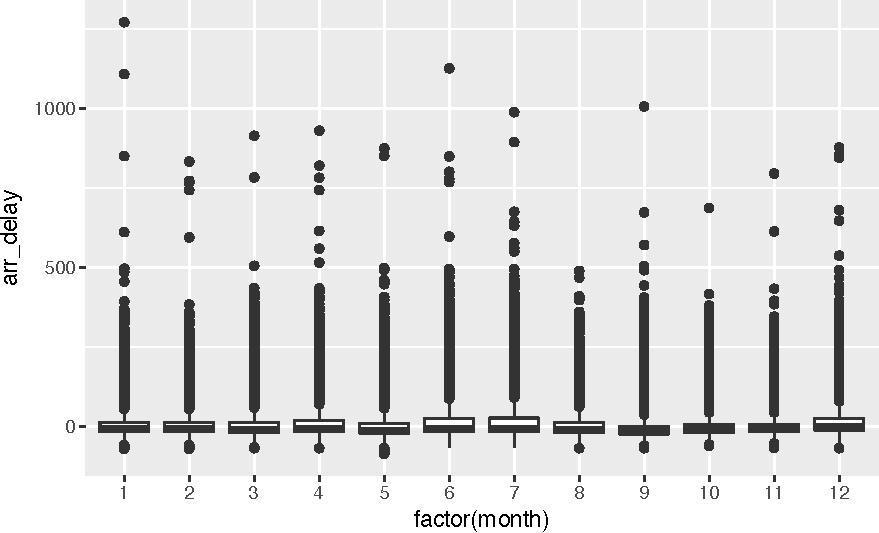
\includegraphics[width=0.7\linewidth]{050_Daten_visualisieren_files/figure-latex/unnamed-chunk-6-1} \end{center}

Schauen wir uns den Befehl \texttt{qplot} etwas näher an. Wie ist er
aufgebaut?

\BeginKnitrBlock{rmdpseudocode}
\texttt{qplot}: Erstelle schnell (q wie quick in \texttt{qplot}) mal
einen Plot (engl. ``plot'': Diagramm).\\
\texttt{x}: Der X-Achse soll die Variable ``carrier'' zugeordnet
werden.\\
\texttt{y}: Der Y-Achse soll die Variable ``arr\_dely'' zugeorndet
werden.\\
\texttt{geom}: (``geometriches Objekt'') Gemalt werden soll ein Boxplot,
nicht etwa Punkte, Linien oder sonstiges.\\
\texttt{data}: Als Datensatz bitte \texttt{flights} verwenden.
\EndKnitrBlock{rmdpseudocode}

Offenbar gibt es viele Extremwerte, was die Verspätung betrifft. Das
erscheint mir nicht unplausibel (Schneesturm im Winter, Flugzeug
verschwunden\ldots{}). Vor dem Hintergrund der Extremwerte erscheinen
die mittleren Verspätungen (Mediane) in den Boxplots als ähnlich.
Vielleicht ist der Unterschied zwischen den Monaten ausgeprägter?

\begin{Shaded}
\begin{Highlighting}[]
\KeywordTok{qplot}\NormalTok{(}\DataTypeTok{x =} \KeywordTok{factor}\NormalTok{(month), }\DataTypeTok{y =} \NormalTok{arr_delay, }\DataTypeTok{geom =} \StringTok{"boxplot"}\NormalTok{, }\DataTypeTok{data =} \NormalTok{flights)}
\end{Highlighting}
\end{Shaded}

\begin{center}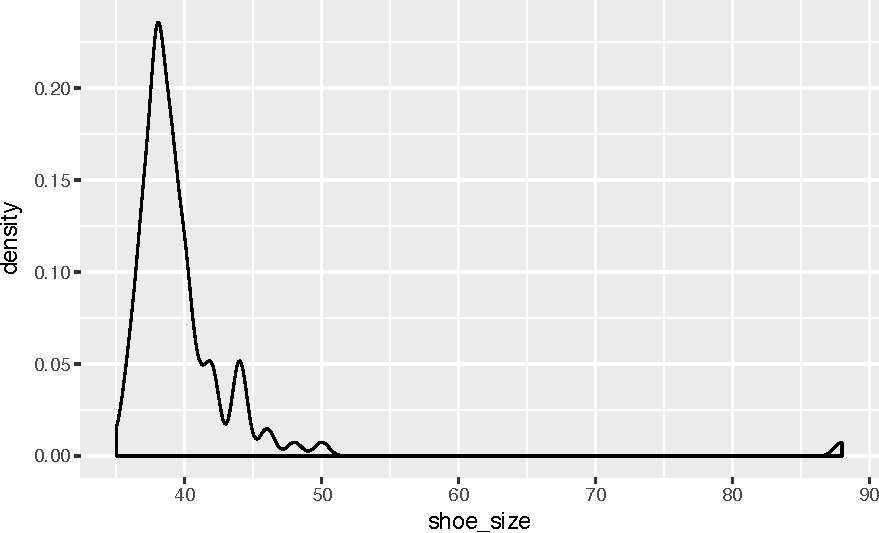
\includegraphics[width=0.7\linewidth]{050_Daten_visualisieren_files/figure-latex/unnamed-chunk-7-1} \end{center}

Kaum Unterschied; das spricht gegen die Schneesturm-Idee als Grund für
Verspätung. Aber schauen wir uns zuerst die Syntax von \texttt{qplot}
näher an. ``q'' in \texttt{qplot} steht für ``quick''. Tatsächlich hat
\texttt{qplot} einen großen Bruder, \texttt{ggplot}\footnote{Achtung:
  Nicht \texttt{qqplot}, nicht \texttt{ggplot2}, nicht
  \texttt{gplot}\ldots{}}, der deutlich mehr Funktionen aufweist - und
daher auch die umfangreichere (=komplexere) Syntax. Fangen wir mit
\texttt{qplot} an.

Diese Syntax des letzten Beispiels ist recht einfach, nämlich:

\begin{Shaded}
\begin{Highlighting}[]
\KeywordTok{qplot} \NormalTok{(}\DataTypeTok{x =} \NormalTok{X_Achse, }\DataTypeTok{y =} \NormalTok{Y_Achse, }\DataTypeTok{data =} \NormalTok{mein_dataframe, }\DataTypeTok{geom =} \StringTok{"ein_geom"}\NormalTok{)}
\end{Highlighting}
\end{Shaded}

Wir definieren mit \texttt{x}, welche Variable der X-Achse des Diagramms
zugewiesen werden soll, z.B. \texttt{month}; analog mit Y-Achse. Mit
\texttt{data} sagen wir, in welchem Dataframe die Spalten ``wohnen'' und
als ``geom'' ist die Art des statistischen ``\emph{geom}etrischen
Objects'' gemeint, also Punkte, Linien, Boxplots, Balken\ldots{}

\section{Häufige Arten von
Diagrammen}\label{haufige-arten-von-diagrammen}

Unter den vielen Arten von Diagrammen und vielen Arten, diese zu
klassifizieren greifen wir uns ein paar häufige Diagramme heraus und
schauen uns diese der Reihe nach an.

\subsection{Eine kontinuierliche
Variable}\label{eine-kontinuierliche-variable}

Schauen wir uns die Verteilung der Schuhgrößen von Studierenden an.

\begin{Shaded}
\begin{Highlighting}[]
\NormalTok{wo_men <-}\StringTok{ }\KeywordTok{read.csv}\NormalTok{(}\StringTok{"data/wo_men.csv"}\NormalTok{)}

\KeywordTok{qplot}\NormalTok{(}\DataTypeTok{x =} \NormalTok{shoe_size, }\DataTypeTok{data =} \NormalTok{wo_men)}
\end{Highlighting}
\end{Shaded}

\begin{center}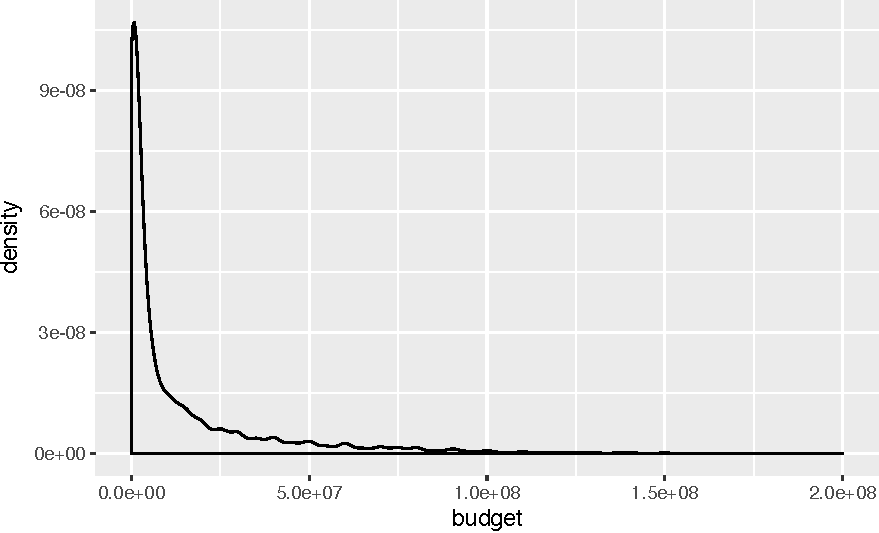
\includegraphics[width=0.7\linewidth]{050_Daten_visualisieren_files/figure-latex/unnamed-chunk-9-1} \end{center}

Weisen wir nur der X-Achse (aber nicht der Y-Achse) eine kontinuierliche
Variable zu, so wählt \texttt{ggplot2} automatisch als Geom automatisch
ein Histogramm; wir müssen daher nicht explizieren, dass wir ein
Histogramm als Geom wünschen (aber wir könnten es hinzufügen).
Alternativ wäre ein Dichtediagramm hier von Interesse:

\begin{Shaded}
\begin{Highlighting}[]
\CommentTok{# qplot(x = shoe_size, data = wo_men)  wie oben}

\KeywordTok{qplot}\NormalTok{(}\DataTypeTok{x =} \NormalTok{shoe_size, }\DataTypeTok{data =} \NormalTok{wo_men, }\DataTypeTok{geom =} \StringTok{"density"}\NormalTok{)}
\end{Highlighting}
\end{Shaded}

\begin{center}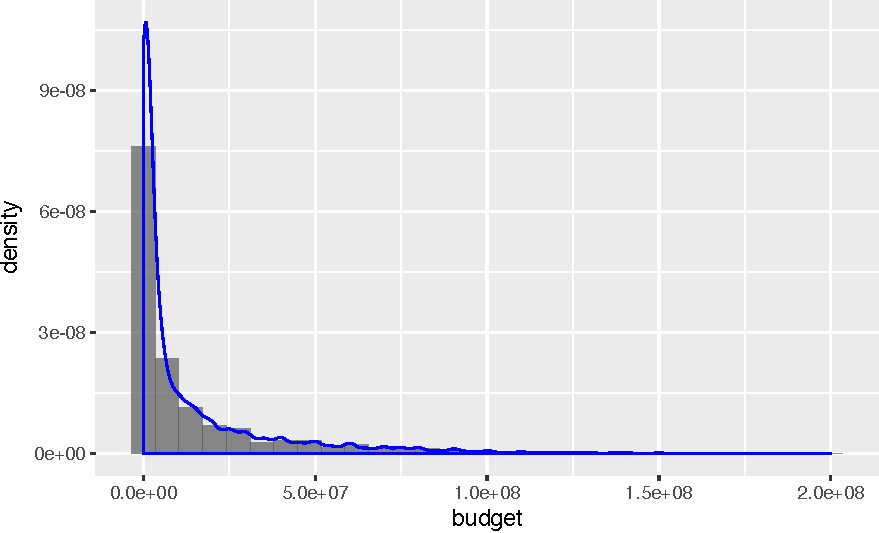
\includegraphics[width=0.7\linewidth]{050_Daten_visualisieren_files/figure-latex/unnamed-chunk-10-1} \end{center}

Was man sich merken muss, ist, dass hier nur das Geom mit
Anführungsstrichen zu benennen ist, die übrigen Parameter \emph{ohne}.

Vielleicht wäre es noch schön, beide Geome zu kombinieren in einem
Diagramm. Das ist etwas komplizierter; wir müssen zum großen Bruder
\texttt{ggplot} umsteigen, da \texttt{qplot} nicht diese Funktionen
anbietet.

\begin{Shaded}
\begin{Highlighting}[]
\KeywordTok{ggplot}\NormalTok{(}\DataTypeTok{data =} \NormalTok{wo_men) +}
\StringTok{  }\KeywordTok{aes}\NormalTok{(}\DataTypeTok{x =} \NormalTok{shoe_size) +}
\StringTok{  }\KeywordTok{geom_histogram}\NormalTok{(}\KeywordTok{aes}\NormalTok{(}\DataTypeTok{y =} \NormalTok{..density..), }\DataTypeTok{alpha =} \NormalTok{.}\DecValTok{7}\NormalTok{) +}
\StringTok{  }\KeywordTok{geom_density}\NormalTok{(}\DataTypeTok{color =} \StringTok{"blue"}\NormalTok{)}
\end{Highlighting}
\end{Shaded}

\begin{center}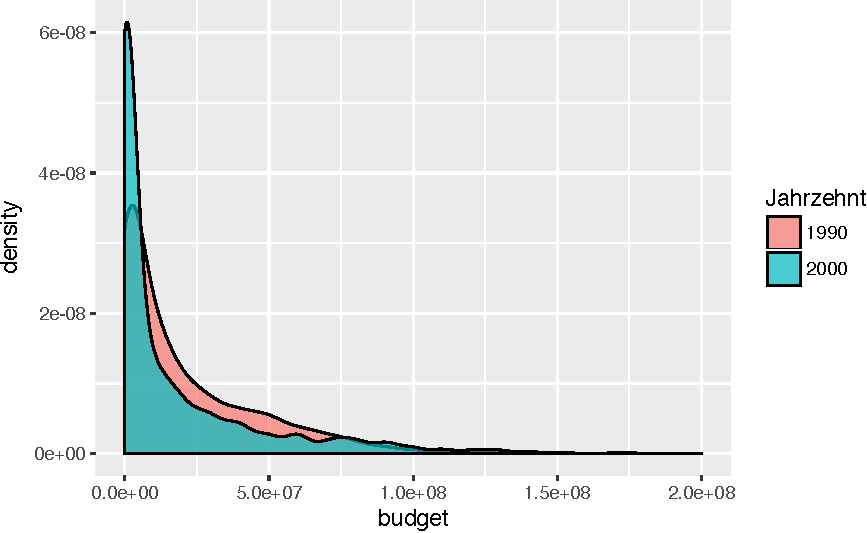
\includegraphics[width=0.7\linewidth]{050_Daten_visualisieren_files/figure-latex/unnamed-chunk-11-1} \end{center}

Zuerst haben wir mit dem Parameter \texttt{data} den Dateframe benannt.
\texttt{aes} definiert, welche Variablen welchen Achsen (oder auch z.B.
Füllfarben) zugewiesen werden. Hier sagen wir, dass die Schuhgröße auf
X-Achse stehen soll. Das \texttt{+}-Zeichen trennt die einzelnen
Bestandteile des \texttt{ggplot}-Aufrufs voneinander. Als nächstes sagen
wir, dass wir gerne ein Histogram hätten: \texttt{geom\_histogram}.
Dabei soll aber nicht wie gewöhnlich auf der X-Achse die Häufigkeit
stehen, sondern die Dichte. \texttt{ggplot} berechnet selbständig die
Dichte und nennt diese Variable \texttt{..density..}; die vielen Punkte
sollen wohl klar machen, dass es sich nicht um eine ``normale'' Variable
aus dem eigenen Dateframe handelt, sondern um eine ``interne'' Varialbe
von \texttt{ggplot} - die wir aber nichtsdestotrotz verwenden können.
\texttt{alpha} bestimmt die ``Durchsichtigkeit'' eines Geoms; spielen
Sie mal etwas damit herum. Schließlich malen wir noch ein blaues
Dichtediagramm \emph{übe}r das Histogramm.

Wünsche sind ein Fass ohne Boden\ldots{} Wäre es nicht schön, ein
Diagramm für Männer und eines für Frauen zu haben, um die Verteilungen
vergleichen zu können?

\begin{Shaded}
\begin{Highlighting}[]
\KeywordTok{qplot}\NormalTok{(}\DataTypeTok{x =} \NormalTok{shoe_size, }\DataTypeTok{data =} \NormalTok{wo_men, }\DataTypeTok{geom =} \StringTok{"density"}\NormalTok{, }\DataTypeTok{color =} \NormalTok{sex)}
\KeywordTok{qplot}\NormalTok{(}\DataTypeTok{x =} \NormalTok{shoe_size, }\DataTypeTok{data =} \NormalTok{wo_men, }\DataTypeTok{geom =} \StringTok{"density"}\NormalTok{, }\DataTypeTok{fill =} \NormalTok{sex, }\DataTypeTok{alpha =} \KeywordTok{I}\NormalTok{(.}\DecValTok{7}\NormalTok{))}
\end{Highlighting}
\end{Shaded}

\begin{center}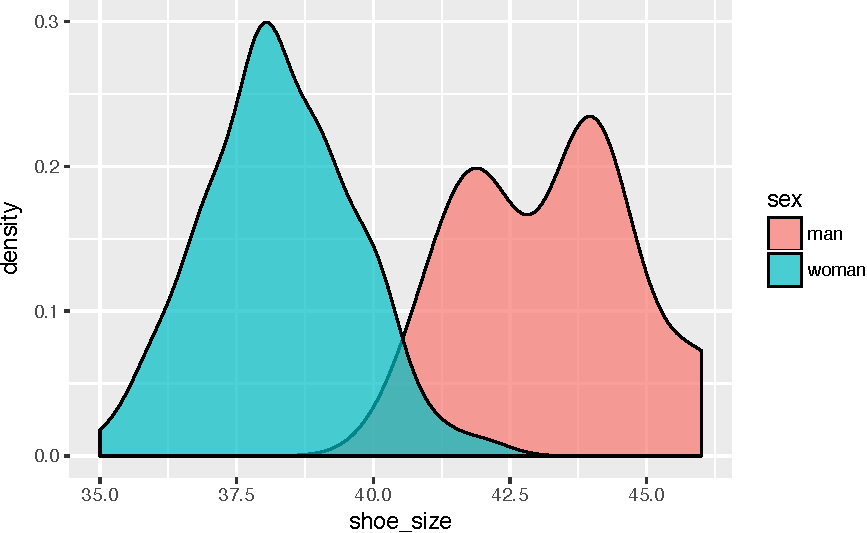
\includegraphics[width=0.7\linewidth]{050_Daten_visualisieren_files/figure-latex/unnamed-chunk-12-1} 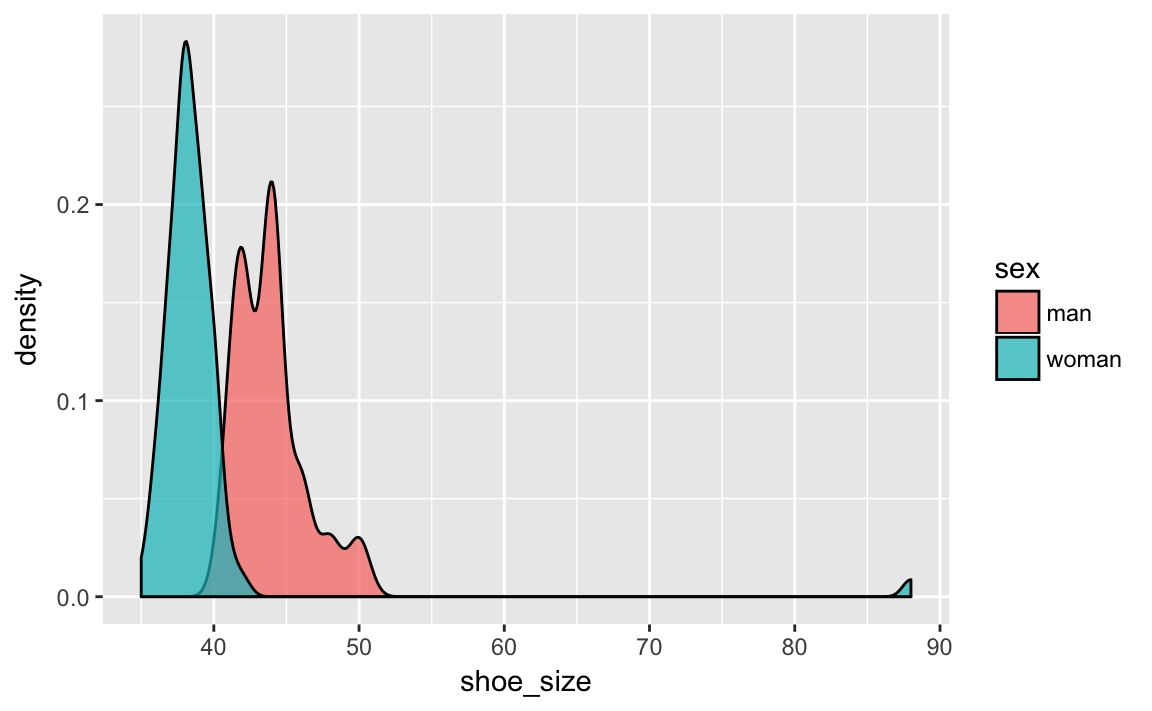
\includegraphics[width=0.7\linewidth]{050_Daten_visualisieren_files/figure-latex/unnamed-chunk-12-2} \end{center}

Hier sollten vielleicht noch die Extremwerte entfernt werden, um den
Blick auf das Gros der Werte nicht zu verstellen:

\begin{Shaded}
\begin{Highlighting}[]

\NormalTok{wo_men %>%}\StringTok{ }
\StringTok{  }\KeywordTok{filter}\NormalTok{(shoe_size <=}\StringTok{ }\DecValTok{47}\NormalTok{) ->}\StringTok{ }\NormalTok{wo_men2}

\KeywordTok{qplot}\NormalTok{(}\DataTypeTok{x =} \NormalTok{shoe_size, }\DataTypeTok{data =} \NormalTok{wo_men2, }\DataTypeTok{geom =} \StringTok{"density"}\NormalTok{, }\DataTypeTok{fill =} \NormalTok{sex, }\DataTypeTok{alpha =} \KeywordTok{I}\NormalTok{(.}\DecValTok{7}\NormalTok{))}
\end{Highlighting}
\end{Shaded}

\begin{center}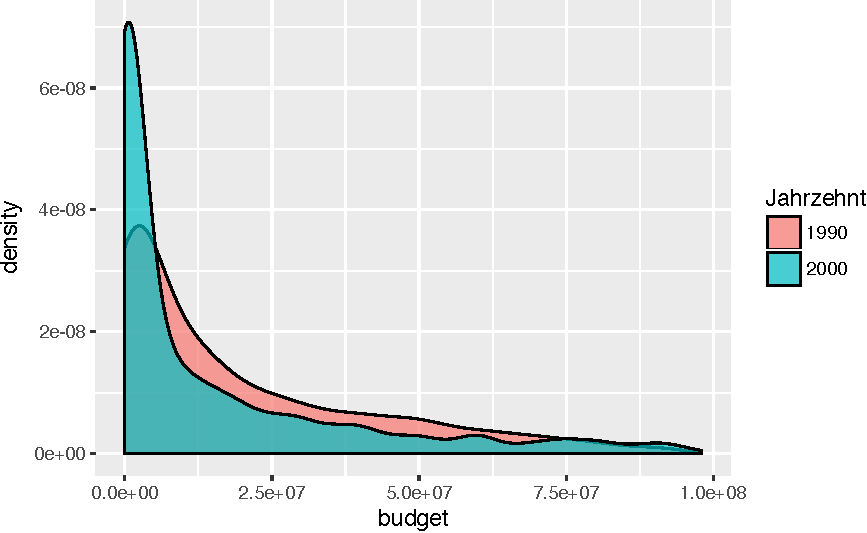
\includegraphics[width=0.7\linewidth]{050_Daten_visualisieren_files/figure-latex/unnamed-chunk-13-1} \end{center}

Besser. Man kann das Durchpfeifen auch bis zu \texttt{qplot}
weiterführen:

\begin{Shaded}
\begin{Highlighting}[]
\NormalTok{wo_men %>%}\StringTok{ }
\StringTok{  }\KeywordTok{filter}\NormalTok{(shoe_size <=}\StringTok{ }\DecValTok{47}\NormalTok{) %>%}\StringTok{ }
\StringTok{  }\KeywordTok{qplot}\NormalTok{(}\DataTypeTok{x =} \NormalTok{shoe_size, }\DataTypeTok{data =} \NormalTok{., }\DataTypeTok{geom =} \StringTok{"density"}\NormalTok{, }\DataTypeTok{fill =} \NormalTok{sex, }\DataTypeTok{alpha =} \KeywordTok{I}\NormalTok{(.}\DecValTok{7}\NormalTok{))}
\end{Highlighting}
\end{Shaded}

\begin{center}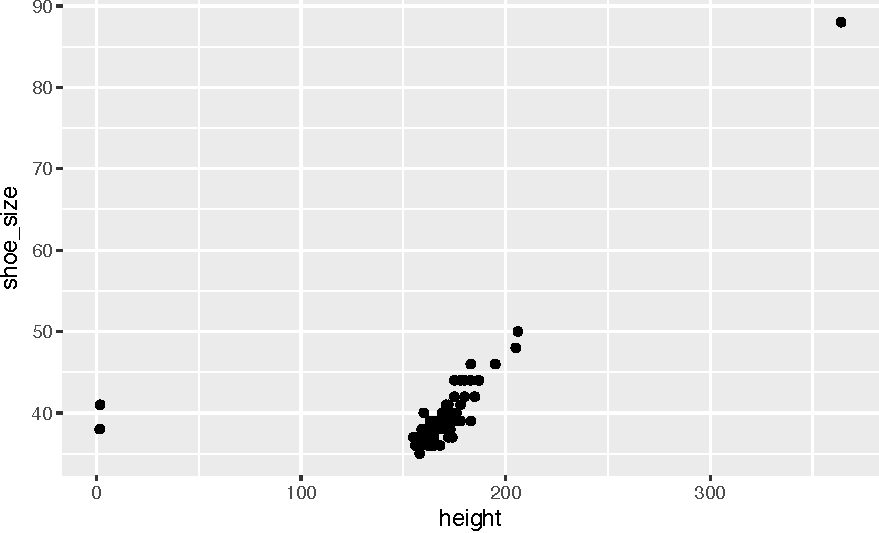
\includegraphics[width=0.7\linewidth]{050_Daten_visualisieren_files/figure-latex/unnamed-chunk-14-1} \end{center}

Die Pfeife versucht im Standard, das Endprodukt des lezten
Arbeitsschritts an den \emph{ersten} Parameter des nächsten Befehls
weiterzugeben. Ein kurzer Blick in die Hilfe von \texttt{qplot} zeigt,
dass der erste Parameter nicht \texttt{data} ist, sondern \texttt{x}.
Daher müssen wir explizit sagen, an welchen Parameter wir das Endprodukt
des lezten Arbeitsschritts geben wollen. Netterweise müssen wir dafür
nicht viel tippen: Mit einem schlichten Punkt \texttt{.} können wir
sagen ``nimm den Dataframe, so wie er vom letzten Arbeitsschritt
ausgegeben wurde''.

Mit \texttt{fill\ =\ sex} sagen wir \texttt{qplot}, dass er für Männer
und Frauen jeweils ein Dichtediagramm erzeugen soll; jedem
Dichtediagramm wird dabei eine Farbe zugewiesen (die uns
\texttt{ggplot2} im Standard voraussucht). Mit anderen Worten: Die Werte
von \texttt{sex} werden der Füllfarbe der Histogramme zugeordnet.
Anstelle der Füllfarbe hätten wir auch die Linienfarbe verwenden können;
die Syntax wäre dann: \texttt{color\ =\ sex}.

\subsection{Zwei kontinuierliche
Variablen}\label{zwei-kontinuierliche-variablen}

Ein Streudiagramm ist die klassiche Art, zwei metrische Variablen
darzustellen. Das ist mit \texttt{qplot} einfach:

\begin{Shaded}
\begin{Highlighting}[]
\KeywordTok{qplot}\NormalTok{(}\DataTypeTok{x =} \NormalTok{height, }\DataTypeTok{y =} \NormalTok{shoe_size, }\DataTypeTok{data =} \NormalTok{wo_men)}
\end{Highlighting}
\end{Shaded}

\begin{center}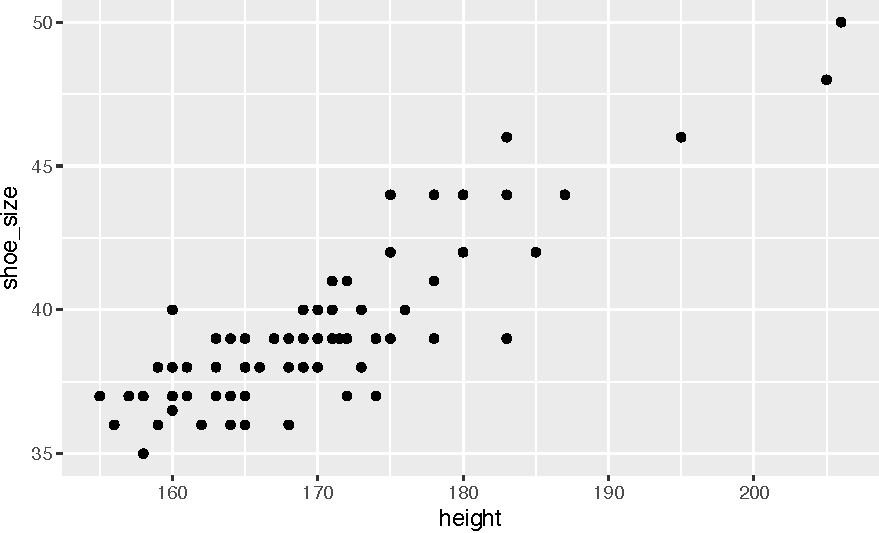
\includegraphics[width=0.7\linewidth]{050_Daten_visualisieren_files/figure-latex/unnamed-chunk-15-1} \end{center}

Wir weisen wieder der X-Achse und der Y-Achse eine Variable zu; handelt
es sich in beiden Fällen um Zahlen, so wählt \texttt{ggplot2}
automatisch ein Streudiagramm - d.h. Punkte als Geom
(\texttt{geom\ =\ "point"}). Wir sollten aber noch die Extremwerte
herausnehmen:

\begin{Shaded}
\begin{Highlighting}[]
\NormalTok{wo_men %>%}\StringTok{ }
\StringTok{  }\KeywordTok{filter}\NormalTok{(height >}\StringTok{ }\DecValTok{150}\NormalTok{, height <}\StringTok{ }\DecValTok{210}\NormalTok{, shoe_size <}\StringTok{ }\DecValTok{55}\NormalTok{) %>%}\StringTok{ }
\StringTok{  }\KeywordTok{qplot}\NormalTok{(}\DataTypeTok{x =} \NormalTok{height, }\DataTypeTok{y =} \NormalTok{shoe_size, }\DataTypeTok{data =} \NormalTok{.)}
\end{Highlighting}
\end{Shaded}

\begin{center}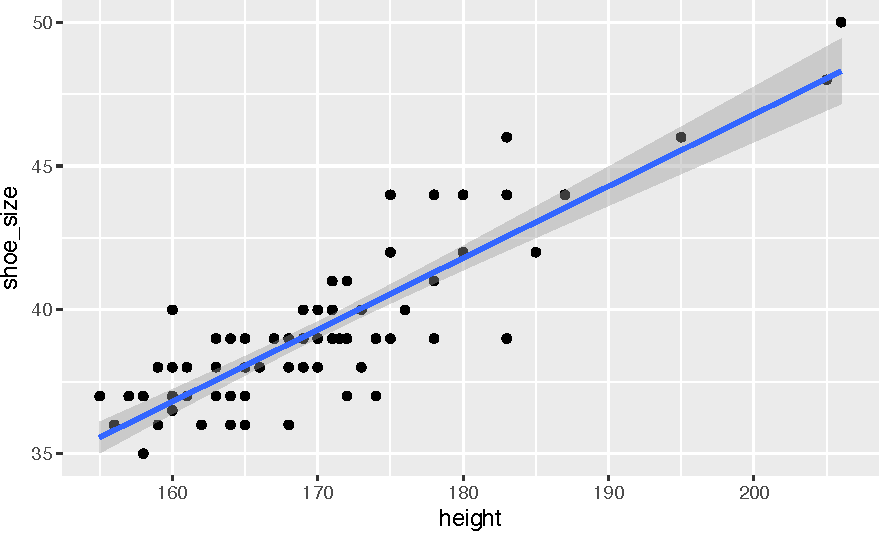
\includegraphics[width=0.7\linewidth]{050_Daten_visualisieren_files/figure-latex/unnamed-chunk-16-1} \end{center}

Der Trend ist deutlich erkennbar: Je größer die Person, desto länger die
Füß´. Zeichnen wir noch eine Trendgerade ein.

\begin{Shaded}
\begin{Highlighting}[]
\NormalTok{wo_men %>%}\StringTok{ }
\StringTok{  }\KeywordTok{filter}\NormalTok{(height >}\StringTok{ }\DecValTok{150}\NormalTok{, height <}\StringTok{ }\DecValTok{210}\NormalTok{, shoe_size <}\StringTok{ }\DecValTok{55}\NormalTok{) %>%}\StringTok{ }
\StringTok{  }\KeywordTok{qplot}\NormalTok{(}\DataTypeTok{x =} \NormalTok{height, }\DataTypeTok{y =} \NormalTok{shoe_size, }\DataTypeTok{data =} \NormalTok{.) +}
\StringTok{  }\KeywordTok{geom_smooth}\NormalTok{(}\DataTypeTok{method =} \StringTok{"lm"}\NormalTok{)}
\end{Highlighting}
\end{Shaded}

\begin{center}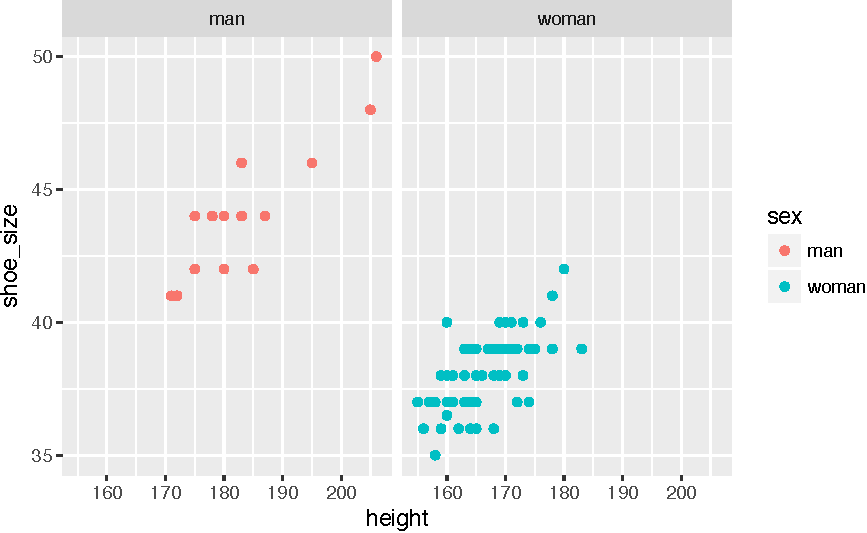
\includegraphics[width=0.7\linewidth]{050_Daten_visualisieren_files/figure-latex/unnamed-chunk-17-1} \end{center}

Synonym könnten wir auch schreiben:

\begin{Shaded}
\begin{Highlighting}[]
\NormalTok{wo_men %>%}\StringTok{ }
\StringTok{  }\KeywordTok{filter}\NormalTok{(height >}\StringTok{ }\DecValTok{150}\NormalTok{, height <}\StringTok{ }\DecValTok{210}\NormalTok{, shoe_size <}\StringTok{ }\DecValTok{55}\NormalTok{) %>%}\StringTok{ }
\StringTok{  }\KeywordTok{ggplot}\NormalTok{() +}
\StringTok{  }\KeywordTok{aes}\NormalTok{(}\DataTypeTok{x =} \NormalTok{height, }\DataTypeTok{y =} \NormalTok{shoe_size) +}
\StringTok{  }\KeywordTok{geom_point}\NormalTok{() +}
\StringTok{  }\KeywordTok{geom_smooth}\NormalTok{(}\DataTypeTok{method =} \StringTok{"lm"}\NormalTok{)}
\end{Highlighting}
\end{Shaded}

Da \texttt{ggplot} als \emph{ersten} Parameter die Daten erwartet, kann
die Pfeife hier problemlos durchgereicht werden. \emph{Innerhalb} eines
\texttt{ggplot}-Aufrufs werden die einzelen Teile durch ein Pluszeichen
\texttt{+} voneinander getrennt. Nachdem wir den Dataframe benannt
haben, definieren wir die Zuweisung der Variablen zu den Achsen mit
\texttt{aes} (``aes'' wie ``aesthetics'', also das ``Sichtbare'' eines
Diagramms, die Achsen etc., werden definiert). Ein ``Smooth-Geom'' ist
eine Linie, die sich schön an die Punkte anschmiegt, in diesem Falls als
Gerade (lineares Modell, \texttt{lm}).

Bei sehr großen Datensätze, sind Punkte unpraktisch, da sie sich
überdecken (``overplotting''). Ein Abhilfe ist es, die Punkte nur
``schwach'' zu färben. Dazu stellt man die ``Füllstärke'' der Punkte
über \texttt{alpha} ein: \texttt{geom\_point(alpha\ =\ 1/100)}. Um einen
passablen Alpha-Wert zu finden, bedarf es häufig etwas Probierens. Zu
beachten ist, dass es mitunter recht lange dauert, wenn \texttt{ggplot}
viele (\textgreater{}100.000) Punkte malen soll.

Bei noch größeren Datenmengen bietet sich an, den Scatterplot als
``Schachbrett'' aufzufassen, und das Raster einzufärben, je nach Anzahl
der Punkte pro Schachfeld; zwei Geome dafür sind \texttt{geom\_hex()}
und \texttt{geom\_bin2d()}.

\begin{Shaded}
\begin{Highlighting}[]
\KeywordTok{data}\NormalTok{(flights, }\DataTypeTok{package =} \StringTok{"nycflights13"}\NormalTok{)}
\KeywordTok{nrow}\NormalTok{(flights)  }\CommentTok{# groß!}
\CommentTok{#> [1] 336776}

\KeywordTok{ggplot}\NormalTok{(flights) +}
\StringTok{  }\KeywordTok{aes}\NormalTok{(}\DataTypeTok{x =} \NormalTok{distance, }\DataTypeTok{y =} \NormalTok{air_time) +}
\StringTok{  }\KeywordTok{geom_hex}\NormalTok{()}
\end{Highlighting}
\end{Shaded}

\begin{center}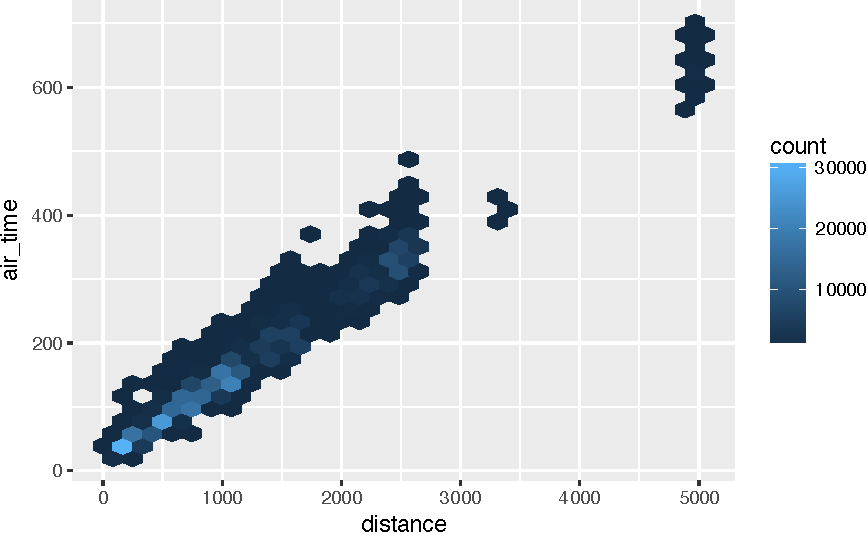
\includegraphics[width=0.7\linewidth]{050_Daten_visualisieren_files/figure-latex/flights_hexbin-1} \end{center}

Wenn man dies verdaut hat, wächst der Hunger nach einer Aufteilung in
Gruppen.

\begin{Shaded}
\begin{Highlighting}[]
\NormalTok{wo_men %>%}\StringTok{ }
\StringTok{  }\KeywordTok{filter}\NormalTok{(height >}\StringTok{ }\DecValTok{150}\NormalTok{, height <}\StringTok{ }\DecValTok{210}\NormalTok{, shoe_size <}\StringTok{ }\DecValTok{55}\NormalTok{) %>%}\StringTok{ }
\StringTok{  }\KeywordTok{qplot}\NormalTok{(}\DataTypeTok{x =} \NormalTok{height, }\DataTypeTok{y =} \NormalTok{shoe_size, }\DataTypeTok{color =} \NormalTok{sex, }\DataTypeTok{data =} \NormalTok{.)}
\end{Highlighting}
\end{Shaded}

\begin{center}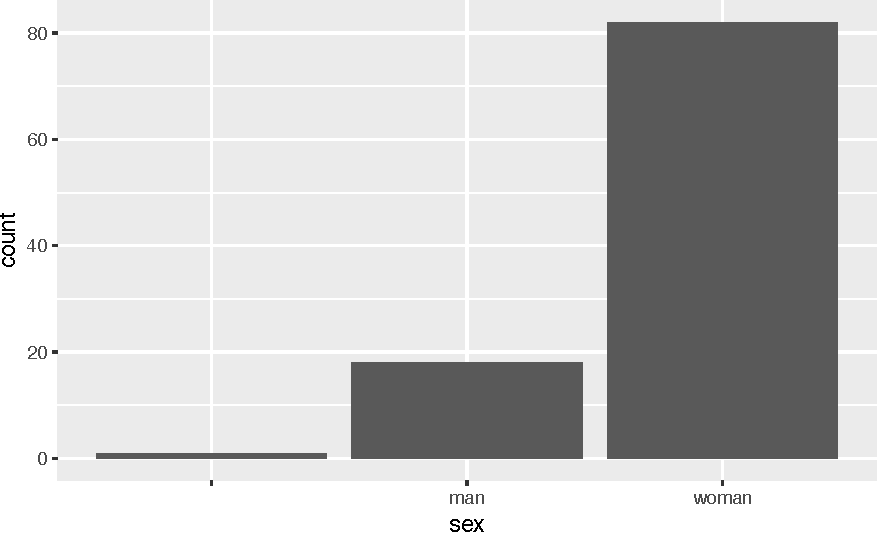
\includegraphics[width=0.7\linewidth]{050_Daten_visualisieren_files/figure-latex/unnamed-chunk-19-1} \end{center}

Mit \texttt{color\ =\ sex} sagen wir, dass die Linienfarbe (der Punkte)
entsprechend der Stufen von \texttt{sex} eingefärbt werden sollen. Die
genaue Farbwahl übernimmt \texttt{ggplot2} für uns.

\subsection{Eine diskrete Variable}\label{eine-diskrete-variable}

Bei diskreten Variablen, vor allem nominalen Variablen, geht es in der
Regel darum, Häufigkeiten auszuzählen. Wie viele Männer und Frauen sind
in dem Datensatz?

\begin{Shaded}
\begin{Highlighting}[]
\KeywordTok{qplot}\NormalTok{(}\DataTypeTok{x =} \NormalTok{sex, }\DataTypeTok{data =} \NormalTok{wo_men)}
\end{Highlighting}
\end{Shaded}

\begin{center}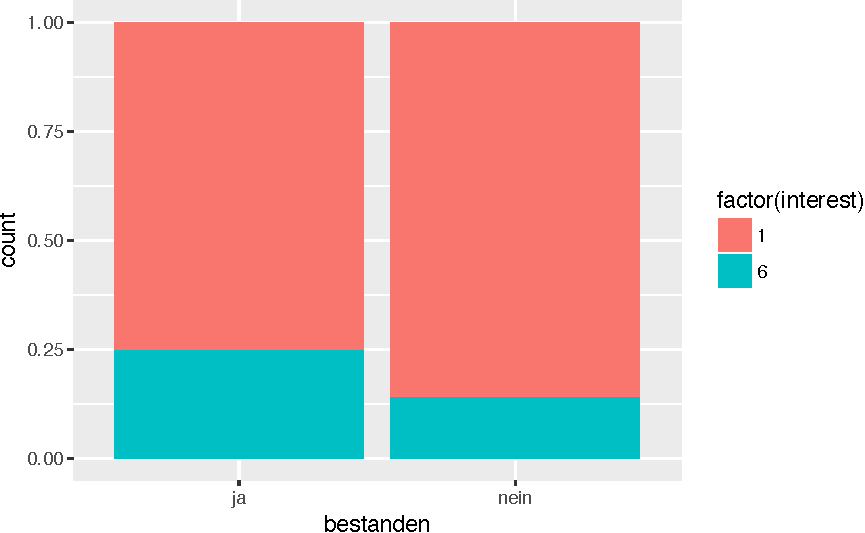
\includegraphics[width=0.7\linewidth]{050_Daten_visualisieren_files/figure-latex/unnamed-chunk-20-1} \end{center}

Falls nur die X-Achse definiert ist und dort eine Faktorvariable oder
eine Text-Variable steht, dann nimmt \texttt{qplot} automatisch ein
Balkendiagramm als Geom.

Entfernen wir vorher noch die fehlenden Werte:

\begin{Shaded}
\begin{Highlighting}[]
\NormalTok{wo_men %>%}\StringTok{ }
\StringTok{  }\KeywordTok{na.omit}\NormalTok{() %>%}\StringTok{ }
\StringTok{  }\KeywordTok{qplot}\NormalTok{(}\DataTypeTok{x =} \NormalTok{sex, }\DataTypeTok{data =} \NormalTok{.)}
\end{Highlighting}
\end{Shaded}

\begin{center}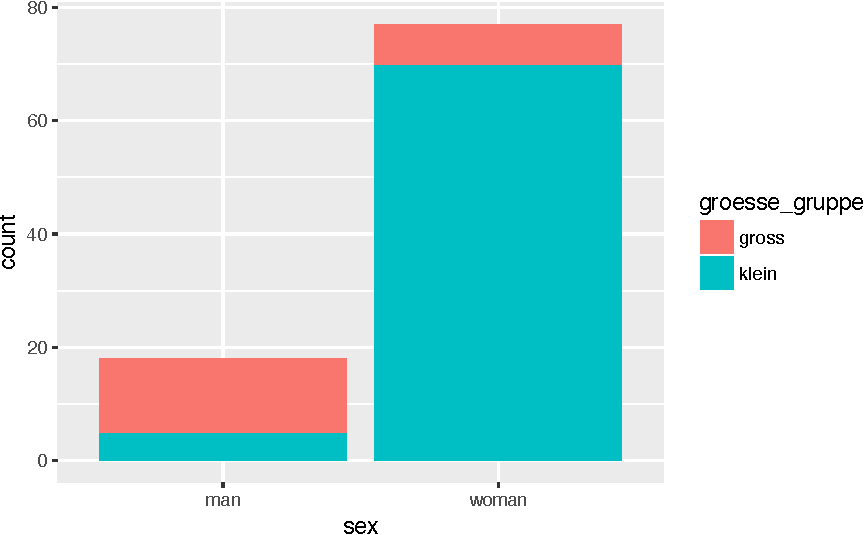
\includegraphics[width=0.7\linewidth]{050_Daten_visualisieren_files/figure-latex/unnamed-chunk-21-1} \end{center}

Wir könnten uns jetzt die Frage stellen, wie viele kleine und viele
große Menschen es bei Frauen und bei den Männern gibt. Dazu müssen wir
zuerst eine Variable wie ``Größe gruppiert'' erstellen mit zwei Werten:
``klein'' und ``groß''. Nennen wir sie \texttt{groesse\_gruppe}

\begin{Shaded}
\begin{Highlighting}[]
\NormalTok{wo_men$groesse_gruppe <-}\StringTok{ }\NormalTok{car::}\KeywordTok{recode}\NormalTok{(wo_men$height, }\StringTok{"lo:175 = 'klein'; else = 'gross'"}\NormalTok{)}

\NormalTok{wo_men %>%}\StringTok{ }
\StringTok{  }\KeywordTok{filter}\NormalTok{(height >}\StringTok{ }\DecValTok{150}\NormalTok{, height <}\StringTok{ }\DecValTok{210}\NormalTok{, shoe_size <}\StringTok{ }\DecValTok{55}\NormalTok{) %>%}\StringTok{ }
\StringTok{  }\NormalTok{na.omit ->}\StringTok{ }\NormalTok{wo_men2}
  
\KeywordTok{qplot}\NormalTok{(}\DataTypeTok{x =} \NormalTok{sex, }\DataTypeTok{fill =} \NormalTok{groesse_gruppe, }\DataTypeTok{data =} \NormalTok{wo_men2)}
\end{Highlighting}
\end{Shaded}

\begin{center}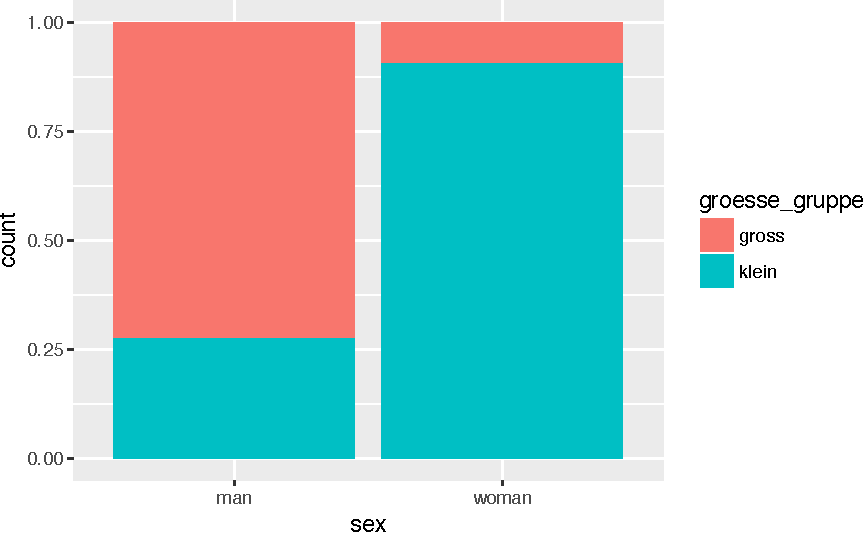
\includegraphics[width=0.7\linewidth]{050_Daten_visualisieren_files/figure-latex/unnamed-chunk-22-1} \end{center}

In Worten sagt der \texttt{recode}-Befehl hier in etwa: ``Kodiere
\texttt{wo\_men\$height} um, und zwar vom kleinsten (\texttt{lo}) Wert
bis 170 soll den Wert \texttt{klein} bekommen, ansonsten bekommt eine
Größe den Wert \texttt{gross}''.

Hier haben wir \texttt{qplot} gesagt, dass der die Balken entsprechend
der Häufigkeit von \texttt{groesse\_gruppe} füllen soll. Und bei den
Frauen sind bei dieser Variablen die Wete \texttt{klein} häufig; bei den
Männern hingegen die Werte \texttt{gross}.

Schön wäre noch, wenn die Balken Prozentwerte angeben würden. Das geht
mit \texttt{qplot} (so) nicht; wir schwenken auf \texttt{ggplot}
um\footnote{Cleveland fände diese Idee nicht so gut.}.

\begin{Shaded}
\begin{Highlighting}[]
\NormalTok{wo_men2 %>%}\StringTok{ }
\StringTok{  }\KeywordTok{ggplot}\NormalTok{() +}
\StringTok{  }\KeywordTok{aes}\NormalTok{(}\DataTypeTok{x =} \NormalTok{sex, }\DataTypeTok{fill =} \NormalTok{groesse_gruppe) +}
\StringTok{  }\KeywordTok{geom_bar}\NormalTok{(}\DataTypeTok{position =} \StringTok{"fill"}\NormalTok{)}
\end{Highlighting}
\end{Shaded}

\begin{center}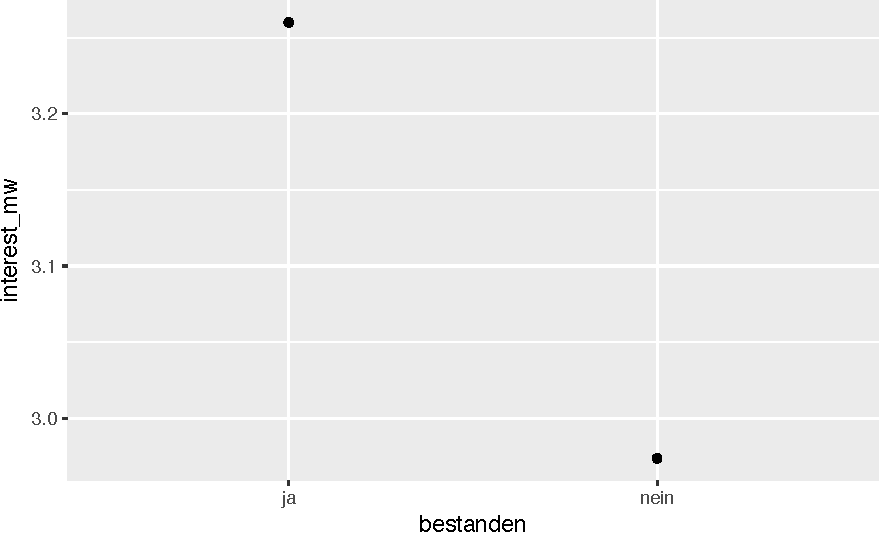
\includegraphics[width=0.7\linewidth]{050_Daten_visualisieren_files/figure-latex/unnamed-chunk-23-1} \end{center}

Schauen wir uns die Struktur des Befehls \texttt{ggplot} näher an.

\BeginKnitrBlock{rmdpseudocode}
\texttt{wo\_men2}: Hey R, nimm den Datensatz \texttt{wo\_men2} UND
DANN\ldots{}\\
\texttt{ggpplot()} : Hey R, male ein Diagramm von Typ ggplot (mit dem
Datensatz aus dem vorherigen Pfeifen-Schritt, d.h. aus der vorherigen
Zeile, also \texttt{wo\_men2})!\\
\texttt{+}: Das Pluszeichen grenzt die Teile eines ggplot-Befehls
voneinander ab.\\
\texttt{aes}: von ``aethetics'', also welche Variablen des Datensatzes
den sichtbaren Aspekten (v.a. Achsen, Farben) zugeordnet werden.\\
\texttt{x}: Der X-Achse (Achtung, \texttt{x} wird klein geschrieben
hier) wird die Variable \texttt{sex} zugeordnet.\\
\texttt{y}: gibt es nicht??? Wenn in einem ggplot-Diagramm \emph{keine}
Y-Achse definiert wird, wird ggplot automatisch ein Histogramm bzw. ein
Balkendiagramm erstellen. Bei diesen Arten von Diagrammen steht auf der
Y-Achse keine eigene Variable, sondern meist die Häufigkeit des
entsprechenden X-Werts (oder eine Funktion der Häufigkeit, wie relative
Häufigkeit).\\
\texttt{fill} Das Diagramm (die Balken) sollen so gefüllt werden, dass
sich die Häufigkeit der Werte von \texttt{groesse\_gruppe} darin
widerspiegelt.\\
\texttt{geom\_XYZ}: Als ``Geom'' soll ein Balken (``bar'') gezeichnet
werden. Ein Geom ist in ggplot2 das zu zeichnende Objekt, also ein
Boxplot, ein Balken, Punkte, Linien etc. Entsprechend wird gewünschte
Geom mit \texttt{geom\_bar}, \texttt{geom\_boxplot},
geom\_point\texttt{etc.\ gewählt.}position =
fill\texttt{:}position\_fill\texttt{will\ sagen,\ dass\ die\ Balken\ alls\ eine\ Höhe\ von\ 100\%\ (1)\ haben.\ Die\ Balken\ zeigen\ also\ nur\ die\ Anteile\ der\ Werte\ der}fill`-Variablen.
\EndKnitrBlock{rmdpseudocode}

Die einzige Änderung in den Parametern ist \texttt{position\ =\ "fill"}.
Dieser Parameter weist \texttt{ggplot} an, die Positionierung der Balken
auf die Darstellung von Anteilen auszulegen. Damit haben alle Balken die
gleiche Höhe, nämlich 100\% (1). Aber die ``Füllung'' der Balken
schwankt je nach der Häufigkeit der Werte von \texttt{groesse\_gruppe}
pro Balken (d.h. pro Wert von \texttt{sex}).

Wir sehen, dass die Anteile von großen bzw. kleinen Menschen bei den
beiden Gruppen (Frauen vs.~Männer) \emph{unterschiedlich hoch} ist. Dies
spricht für einen \emph{Zusammenhang} der beiden Variablen; man sagt,
die Variablen sind \emph{abhängig} (im statistischen Sinne).

\begin{quote}
Je unterschiedlicher die ``Füllhöhe'', desto stärker sind die Variablen
(X-Achse vs.~Füllfarbe) voneinander abhängig (bzw. desto stärker der
Zusammenhang).
\end{quote}

\subsection{Zwei diskrete Variablen}\label{zwei-diskrete-variablen}

Arbeitet man mit nominalen Variablen, so sind Kontingenztabellen Täglich
Brot. Z.B.: Welche Produkte wurden wie häufig an welchem Standort
verkauft? Wie ist die Verteilung von Alkoholkonsum und Körperform bei
Menschen einer Single-Börse. Bleiben wir bei letztem Beispiel.

\begin{Shaded}
\begin{Highlighting}[]
\KeywordTok{data}\NormalTok{(profiles, }\DataTypeTok{package =} \StringTok{"okcupiddata"}\NormalTok{)}

\NormalTok{profiles %>%}\StringTok{ }
\StringTok{  }\KeywordTok{count}\NormalTok{(drinks, body_type) %>%}\StringTok{ }
\StringTok{  }\NormalTok{ggplot +}
\StringTok{  }\KeywordTok{aes}\NormalTok{(}\DataTypeTok{x =} \NormalTok{drinks, }\DataTypeTok{y =} \NormalTok{body_type, }\DataTypeTok{fill =} \NormalTok{n) +}
\StringTok{  }\KeywordTok{geom_tile}\NormalTok{() +}
\StringTok{  }\KeywordTok{theme}\NormalTok{(}\DataTypeTok{axis.text.x =} \KeywordTok{element_text}\NormalTok{(}\DataTypeTok{angle =} \DecValTok{90}\NormalTok{))}
\end{Highlighting}
\end{Shaded}

\begin{center}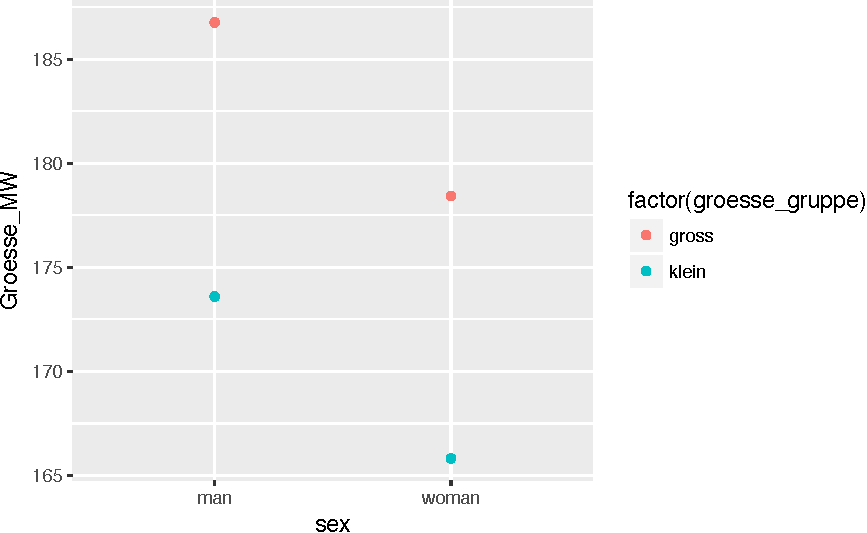
\includegraphics[width=0.7\linewidth]{050_Daten_visualisieren_files/figure-latex/unnamed-chunk-24-1} \end{center}

Was haben wir gemacht? Also:

\BeginKnitrBlock{rmdpseudocode}
Nehme den Datensatz ``profiles'' UND DANN\\
Zähle die Kombinationen von ``drinks'' und ``body\_type'' UND DANN\\
Erstelle ein ggplot-Plot UND DANN\\
Weise der X-Achse ``drinks'' zu, der Y-Achse ``body\_type'' und der
Füllfarbe ``n'' UND DANN\\
Male Fliesen UND DANN\\
Passe das Thema so an, dass der Winkel für Text der X-Achse auf 90 Grad
steht.
\EndKnitrBlock{rmdpseudocode}

Was sofort ins Auge sticht, ist dass ``soziales Trinken'', nennen wir es
mal so, am häfigsten ist, unabhängig von der Körperformm. Ansonsten
scheinen die Zusammenhäng nicht sehr stark zu sein.

\subsection{Zusammenfassungen zeigen}\label{zusammenfassungen-zeigen}

Manchmal möchten wir \emph{nicht} die Rohwerte einer Variablen
darstellen, sondern z.B. die Mittelwerte pro Gruppe. Mittelwerte sind
eine bestimmte \emph{Zusammenfassung} einer Spalte; also fassen wir
zuerst die Körpergröße zum Mittelwert zusammen - gruppiert nach
Geschlecht.

\begin{Shaded}
\begin{Highlighting}[]
\NormalTok{wo_men2 %>%}\StringTok{ }
\StringTok{  }\KeywordTok{group_by}\NormalTok{(sex) %>%}\StringTok{ }
\StringTok{  }\KeywordTok{summarise}\NormalTok{(}\DataTypeTok{Groesse_MW =} \KeywordTok{mean}\NormalTok{(height)) ->}\StringTok{ }\NormalTok{wo_men3}

\NormalTok{wo_men3}
\CommentTok{#> # A tibble: 2 × 2}
\CommentTok{#>      sex Groesse_MW}
\CommentTok{#>   <fctr>      <dbl>}
\CommentTok{#> 1    man        183}
\CommentTok{#> 2  woman        167}
\end{Highlighting}
\end{Shaded}

Diese Tabelle schieben wir jetzt in \texttt{ggplot2}; natürlich hätten
wir das gleich in einem Rutsch durchpfeifen können.

\begin{Shaded}
\begin{Highlighting}[]
\NormalTok{wo_men3 %>%}\StringTok{ }
\StringTok{  }\KeywordTok{qplot}\NormalTok{(}\DataTypeTok{x =} \NormalTok{sex, }\DataTypeTok{y =} \NormalTok{Groesse_MW, }\DataTypeTok{data =} \NormalTok{.)}
\end{Highlighting}
\end{Shaded}

\begin{center}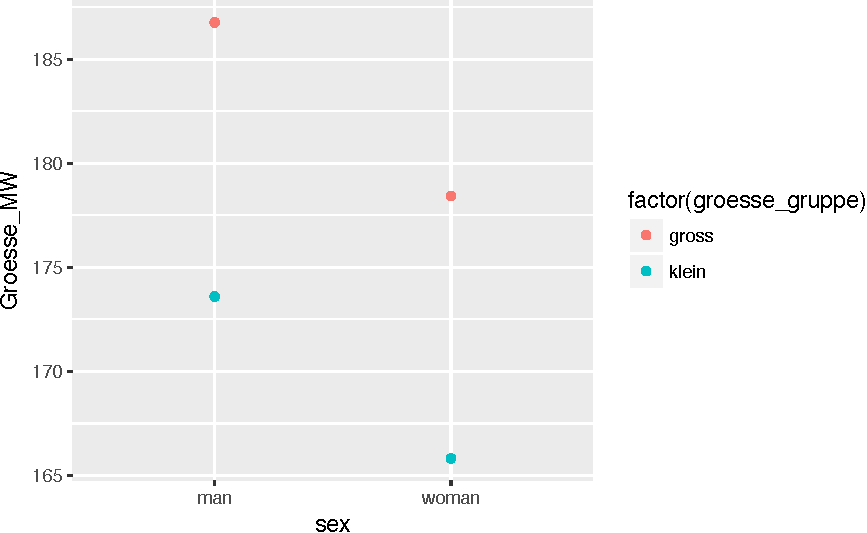
\includegraphics[width=0.7\linewidth]{050_Daten_visualisieren_files/figure-latex/unnamed-chunk-26-1} \end{center}

Das Diagramm besticht nicht durch die Tiefe und Detaillierung. Wenn wir
noch zusätzlich die Mittelwerte nach \texttt{Groesse\_Gruppe} ausweisen,
wird das noch überschaubar bleiben.

\begin{Shaded}
\begin{Highlighting}[]
\NormalTok{wo_men2 %>%}\StringTok{ }
\StringTok{  }\KeywordTok{group_by}\NormalTok{(sex, groesse_gruppe) %>%}\StringTok{ }
\StringTok{  }\KeywordTok{summarise}\NormalTok{(}\DataTypeTok{Groesse_MW =} \KeywordTok{mean}\NormalTok{(height)) %>%}\StringTok{ }
\StringTok{  }\KeywordTok{qplot}\NormalTok{(}\DataTypeTok{x =} \NormalTok{sex, }\DataTypeTok{color =} \KeywordTok{factor}\NormalTok{(groesse_gruppe), }\DataTypeTok{y =} \NormalTok{Groesse_MW, }\DataTypeTok{data =} \NormalTok{.)}
\end{Highlighting}
\end{Shaded}

\begin{center}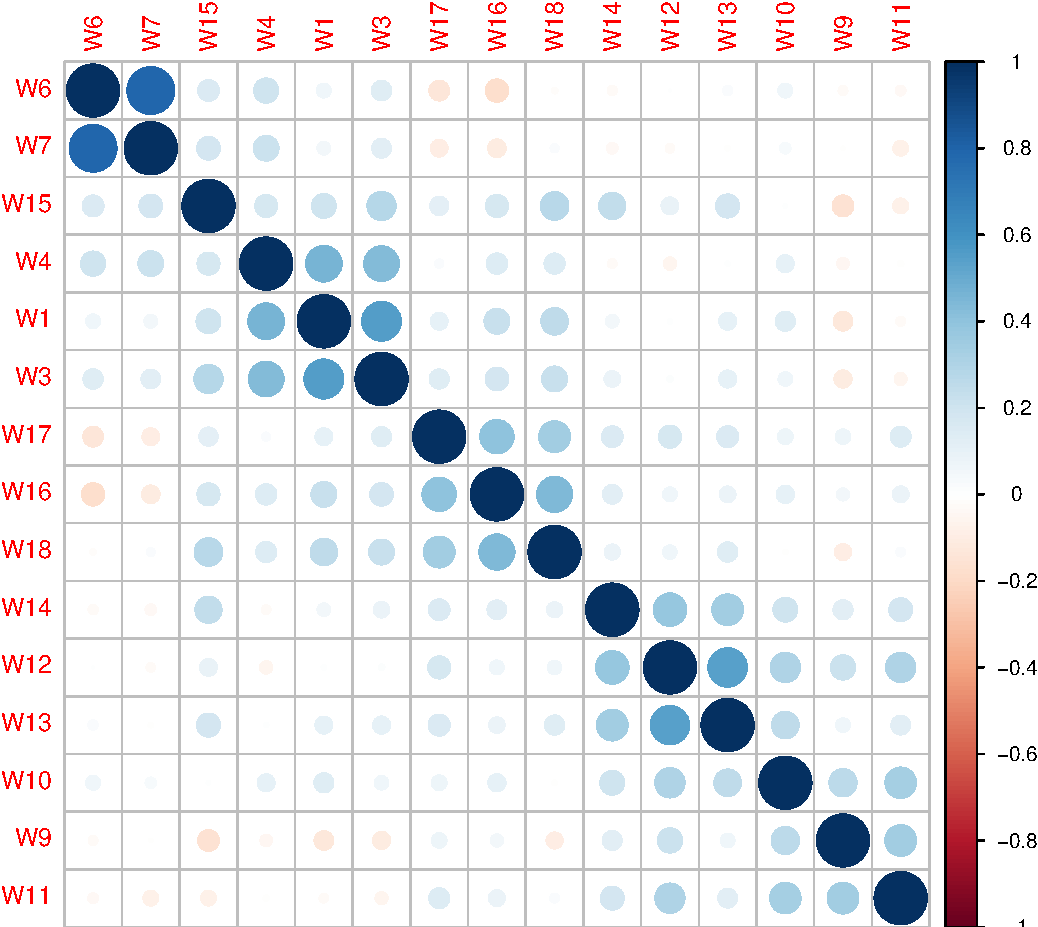
\includegraphics[width=0.7\linewidth]{050_Daten_visualisieren_files/figure-latex/unnamed-chunk-27-1} \end{center}

\section{Farblehre}\label{farblehre}

Erstens, nicht schaden - so könnte hier die Maßregel sein. Es ist
leicht, zu grelle oder wenig kontrastierende Farben auszuwählen. Eine
gute Farbauswahl (Palette) ist nicht so leicht und hängt vom Zweck der
Darstellung ab.

Cynthia Brewer\footnote{\url{http://colorbrewer2.org/\#type=sequential\&scheme=BuGn\&n=3}}
hat einige schöne Farbpaletten zusammengestellt; diese sind in R und in
ggplot2 über das Paket \texttt{RcolorBrewer} verfügbar.

\begin{Shaded}
\begin{Highlighting}[]
\NormalTok{brewer.pal.info %>%}\StringTok{ }\NormalTok{rownames_to_column %>%}\StringTok{ }\KeywordTok{rename}\NormalTok{(}\DataTypeTok{Name =} \NormalTok{rowname) %>%}\StringTok{ }\NormalTok{kable}
\end{Highlighting}
\end{Shaded}

\begin{tabular}{l|r|l|l}
\hline
Name & maxcolors & category & colorblind\\
\hline
BrBG & 11 & div & TRUE\\
\hline
PiYG & 11 & div & TRUE\\
\hline
PRGn & 11 & div & TRUE\\
\hline
PuOr & 11 & div & TRUE\\
\hline
RdBu & 11 & div & TRUE\\
\hline
RdGy & 11 & div & FALSE\\
\hline
RdYlBu & 11 & div & TRUE\\
\hline
RdYlGn & 11 & div & FALSE\\
\hline
Spectral & 11 & div & FALSE\\
\hline
Accent & 8 & qual & FALSE\\
\hline
Dark2 & 8 & qual & TRUE\\
\hline
Paired & 12 & qual & TRUE\\
\hline
Pastel1 & 9 & qual & FALSE\\
\hline
Pastel2 & 8 & qual & FALSE\\
\hline
Set1 & 9 & qual & FALSE\\
\hline
Set2 & 8 & qual & TRUE\\
\hline
Set3 & 12 & qual & FALSE\\
\hline
Blues & 9 & seq & TRUE\\
\hline
BuGn & 9 & seq & TRUE\\
\hline
BuPu & 9 & seq & TRUE\\
\hline
GnBu & 9 & seq & TRUE\\
\hline
Greens & 9 & seq & TRUE\\
\hline
Greys & 9 & seq & TRUE\\
\hline
Oranges & 9 & seq & TRUE\\
\hline
OrRd & 9 & seq & TRUE\\
\hline
PuBu & 9 & seq & TRUE\\
\hline
PuBuGn & 9 & seq & TRUE\\
\hline
PuRd & 9 & seq & TRUE\\
\hline
Purples & 9 & seq & TRUE\\
\hline
RdPu & 9 & seq & TRUE\\
\hline
Reds & 9 & seq & TRUE\\
\hline
YlGn & 9 & seq & TRUE\\
\hline
YlGnBu & 9 & seq & TRUE\\
\hline
YlOrBr & 9 & seq & TRUE\\
\hline
YlOrRd & 9 & seq & TRUE\\
\hline
\end{tabular}

\begin{itemize}
\tightlist
\item
  Kontrastierende Darstellung (nominale/ qualitative Variablen) - z.B.
  Männer vs.~Frauen
\end{itemize}

\begin{Shaded}
\begin{Highlighting}[]
\KeywordTok{display.brewer.all}\NormalTok{(}\DataTypeTok{type=}\StringTok{"qual"}\NormalTok{)}
\end{Highlighting}
\end{Shaded}

\begin{center}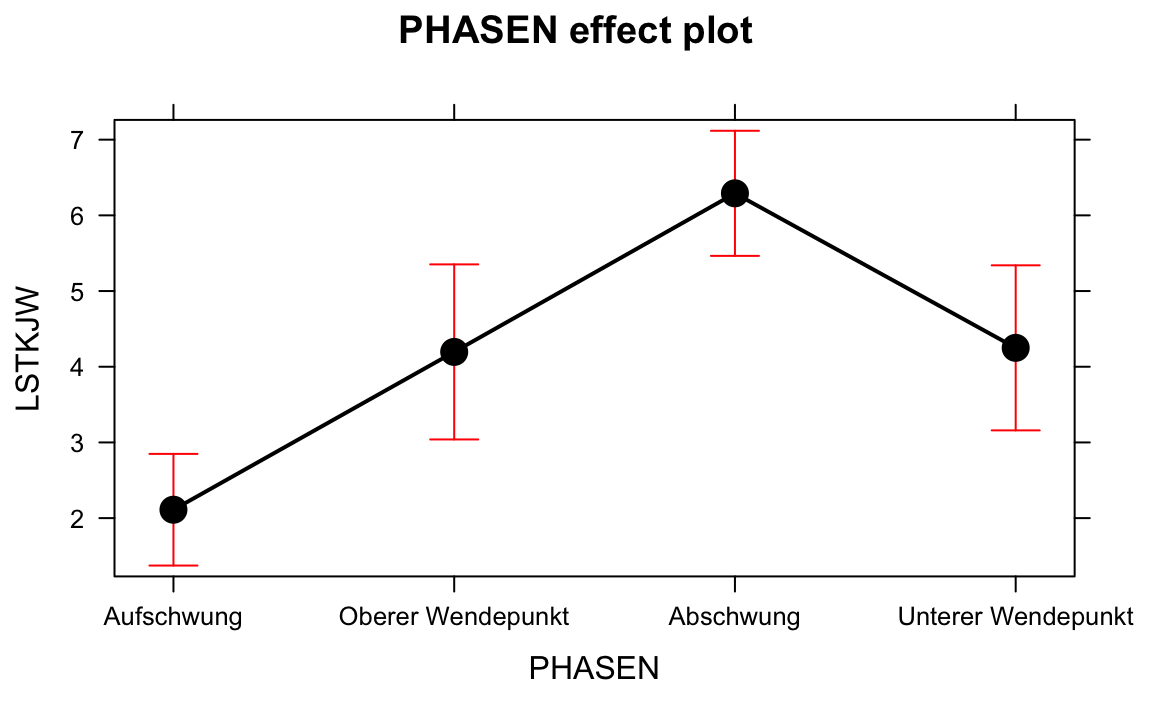
\includegraphics[width=1\linewidth]{050_Daten_visualisieren_files/figure-latex/unnamed-chunk-29-1} \end{center}

\begin{itemize}
\tightlist
\item
  Sequenzielle Darstellung (unipolare numerische Variablen) - z.B. Preis
  oder Häufigkeit
\end{itemize}

\begin{Shaded}
\begin{Highlighting}[]
\KeywordTok{display.brewer.all}\NormalTok{(}\DataTypeTok{type=}\StringTok{"seq"}\NormalTok{)}
\end{Highlighting}
\end{Shaded}

\begin{center}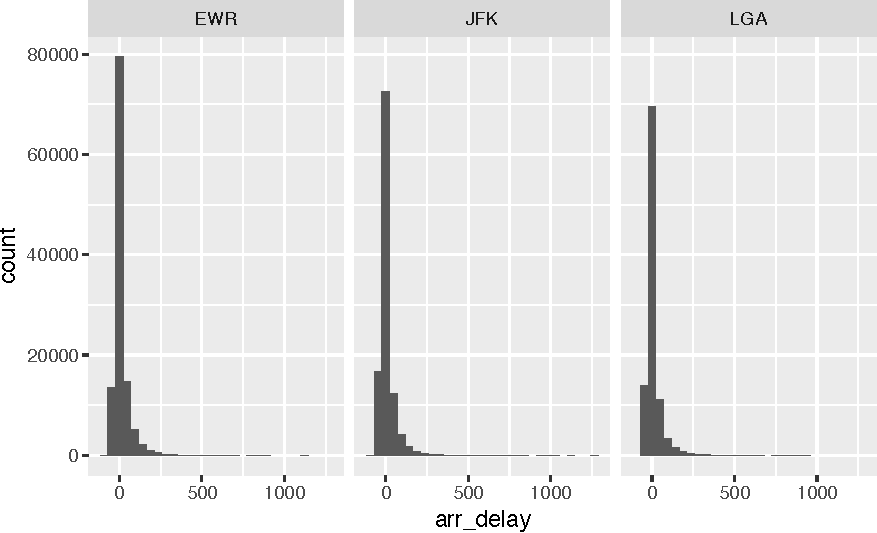
\includegraphics[width=1\linewidth]{050_Daten_visualisieren_files/figure-latex/unnamed-chunk-30-1} \end{center}

\begin{itemize}
\tightlist
\item
  Divergierende Darstellung (bipolare numerische Variablen) - z.B.
  semantische Potenziale oder Abstufung von ``stimme überhaupt nicht
  zu'' über ``neutral'' bis ``stimme voll und ganz zu''
\end{itemize}

\begin{Shaded}
\begin{Highlighting}[]
\KeywordTok{display.brewer.all}\NormalTok{(}\DataTypeTok{type=}\StringTok{"div"}\NormalTok{)}
\end{Highlighting}
\end{Shaded}

\begin{center}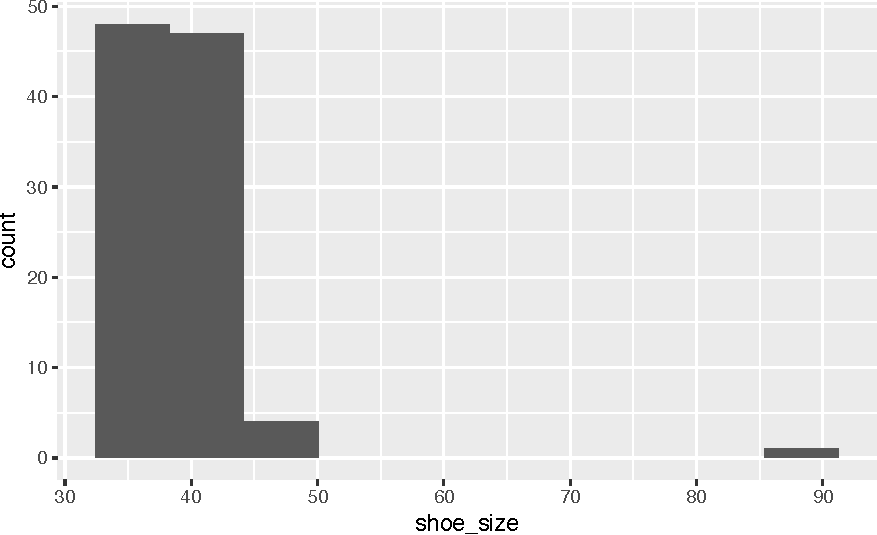
\includegraphics[width=1\linewidth]{050_Daten_visualisieren_files/figure-latex/unnamed-chunk-31-1} \end{center}

In \texttt{ggplot2} können wir folgendermaßen Paletten ändern.

\begin{Shaded}
\begin{Highlighting}[]

\NormalTok{flights %>%}\StringTok{ }
\StringTok{  }\KeywordTok{group_by}\NormalTok{(dest) %>%}\StringTok{ }
\StringTok{  }\KeywordTok{count}\NormalTok{(dest) %>%}\StringTok{ }
\StringTok{  }\KeywordTok{top_n}\NormalTok{(}\DecValTok{5}\NormalTok{)}
\CommentTok{#> # A tibble: 5 × 2}
\CommentTok{#>    dest     n}
\CommentTok{#>   <chr> <int>}
\CommentTok{#> 1   ATL 17215}
\CommentTok{#> 2   BOS 15508}
\CommentTok{#> 3   LAX 16174}
\CommentTok{#> 4   MCO 14082}
\CommentTok{#> 5   ORD 17283}

\NormalTok{p1 <-}\StringTok{ }\NormalTok{flights %>%}\StringTok{ }
\StringTok{  }\KeywordTok{filter}\NormalTok{(dest %in%}\StringTok{ }\KeywordTok{c}\NormalTok{(}\StringTok{"BOS"}\NormalTok{, }\StringTok{"ATL"}\NormalTok{, }\StringTok{"LAX"}\NormalTok{)) %>%}\StringTok{ }
\StringTok{  }\KeywordTok{ggplot}\NormalTok{() +}
\StringTok{  }\KeywordTok{aes}\NormalTok{(}\DataTypeTok{x =} \NormalTok{dest, }\DataTypeTok{y =} \NormalTok{arr_delay, }\DataTypeTok{color =} \NormalTok{dest) +}
\StringTok{  }\KeywordTok{geom_boxplot}\NormalTok{() +}
\StringTok{  }\KeywordTok{scale_color_brewer}\NormalTok{(}\DataTypeTok{palette =} \StringTok{"Set1"}\NormalTok{)}

\NormalTok{p2 <-}\StringTok{ }\NormalTok{flights %>%}\StringTok{ }
\StringTok{  }\KeywordTok{filter}\NormalTok{(dest %in%}\StringTok{ }\KeywordTok{c}\NormalTok{(}\StringTok{"BOS"}\NormalTok{, }\StringTok{"ATL"}\NormalTok{, }\StringTok{"LAX"}\NormalTok{, }\StringTok{"MCO"}\NormalTok{, }\StringTok{"ORD"}\NormalTok{)) %>%}\StringTok{ }
\StringTok{  }\KeywordTok{ggplot}\NormalTok{() +}
\StringTok{  }\KeywordTok{aes}\NormalTok{(}\DataTypeTok{x =} \NormalTok{dest, }\DataTypeTok{y =} \NormalTok{arr_delay, }\DataTypeTok{fill =} \NormalTok{dest) +}
\StringTok{  }\KeywordTok{geom_boxplot}\NormalTok{() +}
\StringTok{  }\KeywordTok{scale_fill_brewer}\NormalTok{(}\DataTypeTok{palette =} \StringTok{"Set1"}\NormalTok{)}

\KeywordTok{grid.arrange}\NormalTok{(p1, p2, }\DataTypeTok{ncol =} \DecValTok{2}\NormalTok{)}
\end{Highlighting}
\end{Shaded}

\begin{center}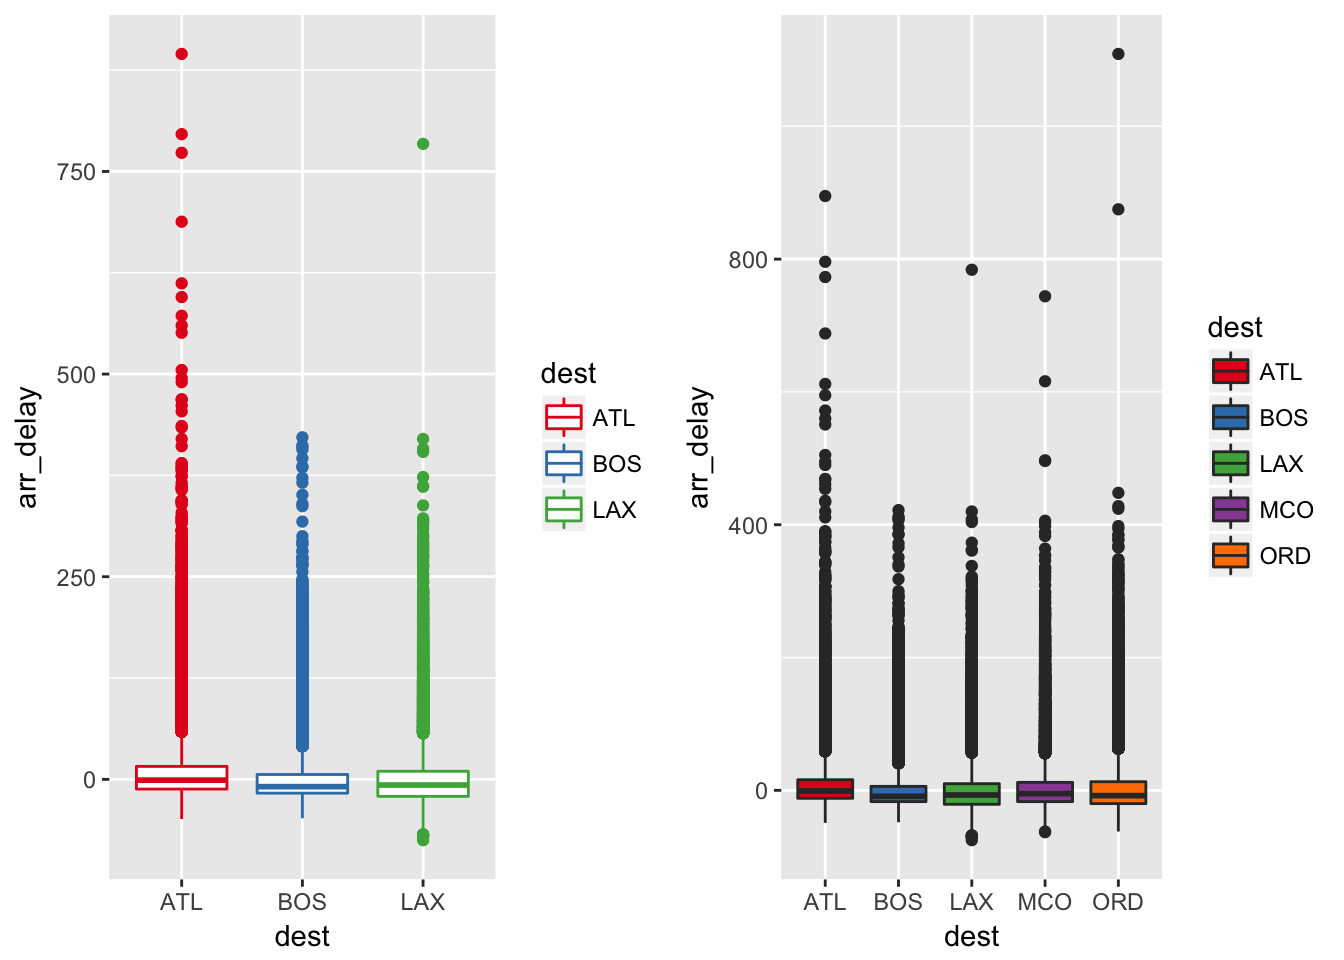
\includegraphics[width=1\linewidth]{050_Daten_visualisieren_files/figure-latex/brewerpal-1} \end{center}

\texttt{scale\_color\_brewer} meint hier: ``Ordne der Variablen, die für
`color' zuständig ist, hier \texttt{sex}, eine Farbe aus der
Brewer-Palette `Set1' zu''. Die Funktion wählt \emph{automatisch} die
richtige Anzahl von Farben.

Man beachte, dass die Linienfarbe über \texttt{color} und die Füllfarbe
über \texttt{fill} zugewiesen wird. Punkte haben nur eine Linienfarbe,
keine Füllfarbe.

Auch die Farbpaletten von Wes Anderson sind erbaulich\footnote{\url{https://github.com/karthik/wesanderson}}.
Diese sind nicht ``hart verdrahtet'' in ggplot2, sondern werden über
\texttt{scale\_XXX\_manual} zugewiesen (wobei XXX z.B. \texttt{color}
oder \texttt{fill} sein kann).

\begin{Shaded}
\begin{Highlighting}[]
\KeywordTok{data}\NormalTok{(tips, }\DataTypeTok{package =} \StringTok{"reshape2"}\NormalTok{)}

\NormalTok{p1 <-}\StringTok{ }\NormalTok{tips %>%}\StringTok{ }
\StringTok{  }\KeywordTok{ggplot}\NormalTok{() +}
\StringTok{  }\KeywordTok{aes}\NormalTok{(}\DataTypeTok{x =} \NormalTok{total_bill, }\DataTypeTok{y =} \NormalTok{tip, }\DataTypeTok{color =} \NormalTok{day) +}
\StringTok{  }\KeywordTok{geom_point}\NormalTok{() +}
\StringTok{  }\KeywordTok{scale_color_manual}\NormalTok{(}\DataTypeTok{values =} \KeywordTok{wes_palette}\NormalTok{(}\StringTok{"GrandBudapest"}\NormalTok{)) +}
\StringTok{  }\KeywordTok{theme}\NormalTok{(}\DataTypeTok{legend.position =} \StringTok{"bottom"}\NormalTok{)}

\NormalTok{p2 <-}\StringTok{ }\NormalTok{tips %>%}\StringTok{ }
\StringTok{  }\KeywordTok{ggplot}\NormalTok{() +}
\StringTok{  }\KeywordTok{aes}\NormalTok{(}\DataTypeTok{x =} \NormalTok{total_bill, }\DataTypeTok{y =} \NormalTok{tip, }\DataTypeTok{color =} \NormalTok{day) +}
\StringTok{  }\KeywordTok{geom_point}\NormalTok{() +}
\StringTok{  }\KeywordTok{scale_color_manual}\NormalTok{(}\DataTypeTok{values =} \KeywordTok{wes_palette}\NormalTok{(}\StringTok{"Chevalier"}\NormalTok{))  +}
\StringTok{  }\KeywordTok{theme}\NormalTok{(}\DataTypeTok{legend.position =} \StringTok{"bottom"}\NormalTok{)}

\NormalTok{meine_farben <-}\StringTok{ }\KeywordTok{c}\NormalTok{(}\StringTok{"red"}\NormalTok{, }\StringTok{"blue"}\NormalTok{, }\StringTok{"#009981"}\NormalTok{, }\StringTok{"#32F122"}\NormalTok{)}

\NormalTok{p3 <-}\StringTok{ }\NormalTok{tips %>%}\StringTok{ }
\StringTok{  }\KeywordTok{ggplot}\NormalTok{() +}
\StringTok{  }\KeywordTok{aes}\NormalTok{(}\DataTypeTok{x =} \NormalTok{total_bill, }\DataTypeTok{y =} \NormalTok{tip, }\DataTypeTok{color =} \NormalTok{day) +}
\StringTok{  }\KeywordTok{geom_point}\NormalTok{() +}
\StringTok{  }\KeywordTok{scale_color_manual}\NormalTok{(}\DataTypeTok{values =} \NormalTok{meine_farben)  +}
\StringTok{  }\KeywordTok{theme}\NormalTok{(}\DataTypeTok{legend.position =} \StringTok{"bottom"}\NormalTok{)}

\KeywordTok{grid.arrange}\NormalTok{(p1, p2, p3, }\DataTypeTok{ncol =} \DecValTok{3}\NormalTok{)}
\end{Highlighting}
\end{Shaded}

\begin{center}\includegraphics[width=0.7\linewidth]{050_Daten_visualisieren_files/figure-latex/unnamed-chunk-32-1} \end{center}

Wer sich berufen fühlt, eigene Farben (oder die seiner Organisation zu
verwenden), kommt auf ähnlichem Weg zu Ziel. Man definiere sich seine
Palette, wobei ausreichend Farben definiert sein müssen. Diese weist man
dann über \texttt{scale\_XXX\_manual} dann zu. Man kann einerseits aus
den in R definierten Farben auswählen\footnote{\url{http://sape.inf.usi.ch/quick-reference/ggplot2/colour}}
oder sich selber die RBG-Nummern (in Hexadezimal-Nummern) heraussuchen.

\section{Erweiterungen für ggplot}\label{erweiterungen-fur-ggplot}

\subsection{ggpairs}\label{ggpairs}

Um eine Streudiagramm-Matrix darzustellen, ist der Befehl
\texttt{GGally::ggpairs} praktisch:

\begin{Shaded}
\begin{Highlighting}[]

\NormalTok{tips %>%}\StringTok{ }
\StringTok{  }\KeywordTok{ggpairs}\NormalTok{(}\KeywordTok{aes}\NormalTok{(}\DataTypeTok{color =} \NormalTok{sex), }\DataTypeTok{columns =} \KeywordTok{c}\NormalTok{(}\StringTok{"total_bill"}\NormalTok{, }\StringTok{"smoker"}\NormalTok{, }\StringTok{"tip"}\NormalTok{))}
\end{Highlighting}
\end{Shaded}

\begin{center}\includegraphics[width=0.7\linewidth]{050_Daten_visualisieren_files/figure-latex/unnamed-chunk-33-1} \end{center}

Dabei gibt man an, welche Variable (hier \texttt{sex}) für die Farben im
Diagramm zuständig sein soll (wir ordnen den Werten von \texttt{sex}
jeweils eine Farbe zu). Mit \texttt{columns} sagen wir, welche Spalten
des Dataframes wir dargestellt haben möchten. Lassen wir diesen
Parameter weg, so werden alle Spaltne des Dataframes dargestellt.

\subsection{Correlationsplots}\label{correlationsplots}

Mit dem Paket \texttt{corrr} lassen sich mehrere
Korrelationskoeffizienten auf einmal visualisieren.

\begin{Shaded}
\begin{Highlighting}[]
\NormalTok{df <-}\StringTok{ }\KeywordTok{read.csv}\NormalTok{(}\StringTok{"https://osf.io/meyhp/?action=download"}\NormalTok{)}

\KeywordTok{library}\NormalTok{(corrr)}

\NormalTok{df %>%}\StringTok{ }
\StringTok{  }\KeywordTok{select}\NormalTok{(i01:i10) %>%}\StringTok{   }\CommentTok{# Spalten wählen}
\StringTok{  }\KeywordTok{correlate}\NormalTok{() %>%}\StringTok{   }\CommentTok{# Korrelationsmatrix berechnen}
\StringTok{  }\KeywordTok{rearrange}\NormalTok{() %>%}\StringTok{   }\CommentTok{# Korrelation der Stärke nach ordnen  }
\StringTok{  }\KeywordTok{shave}\NormalTok{() %>%}\StringTok{   }\CommentTok{# das obere Dreieck ist redundant, rasieren wir ab}
\StringTok{  }\KeywordTok{rplot}\NormalTok{()  }\CommentTok{# plotten}
\end{Highlighting}
\end{Shaded}

\begin{figure}

{\centering \includegraphics[width=0.7\linewidth]{050_Daten_visualisieren_files/figure-latex/unnamed-chunk-34-1} 

}

\caption{Korr}\label{fig:unnamed-chunk-34}
\end{figure}

\subsection{Weitere}\label{weitere}

Hier finden sich viele weitere Ergänzungen für ggplot2:
\url{https://www.ggplot2-exts.org}

\section{Fallstudie Extraversion}\label{fallstudie-extraversion}

Eine recht häufige Art von Daten in der Wirtschaft kommen von Umfragen
in der Belegschaft. Diese Daten gilt es dann aufzubereiten und graphisch
wiederzugeben.

\subsection{Daten einlesen}\label{daten-einlesen}

Hier laden wir einen Datensatz zu einer Online-Umfrage:

\begin{Shaded}
\begin{Highlighting}[]
\NormalTok{data <-}\StringTok{ }\KeywordTok{read.csv}\NormalTok{(}\StringTok{"https://osf.io/meyhp/?action=download"}\NormalTok{)}
\end{Highlighting}
\end{Shaded}

Der DOI für diesen Datensatz ist 10.17605/OSF.IO/4KGZH.

Der Datensatz besteht aus 10 Extraversions-Items (B5T nach
Satow\footnote{\url{https://www.zpid.de/pub/tests/PT_9006357_B5T_Forschungsbericht.pdf}})
sowie einigen Verhaltenskorrelaten (zumindest angenommenen). Uns
interessieren also hier nur die 10 Extraversions-Items, die zusammen
Extraversion als Persönlichkeitseigenschaft messen (sollen). Wir werden
die Antworte der Befragten darstelle, aber uns hier keine Gedanken über
Messqualität u.a. machen.

Die Umfrage kann hier\footnote{\url{https://docs.google.com/forms/d/e/1FAIpQLSfD4wQuhDV_edx1WBfN3Qos7XqoVbe41VpiKLRKtGLeuUD09Q/viewform}}
eingesehen werden. Schauen wir uns die Daten mal an:

\begin{Shaded}
\begin{Highlighting}[]
\KeywordTok{glimpse}\NormalTok{(data)}
\CommentTok{#> Observations: 501}
\CommentTok{#> Variables: 28}
\CommentTok{#> $ X                  <int> 1, 2, 3, 4, 5, 6, 7, 8, 9, 10, 11, 12, 13, ...}
\CommentTok{#> $ timestamp          <fctr> 11.03.2015 19:17:48, 11.03.2015 19:18:05, ...}
\CommentTok{#> $ code               <fctr> HSC, ERB, ADP, KHB, PTG, ABL, ber, hph, IH...}
\CommentTok{#> $ i01                <int> 3, 2, 3, 3, 4, 3, 4, 3, 4, 4, 3, 3, 4, 4, 3...}
\CommentTok{#> $ i02r               <int> 3, 2, 4, 3, 3, 2, 4, 3, 4, 4, 3, 4, 3, 3, 3...}
\CommentTok{#> $ i03                <int> 3, 1, 1, 2, 1, 1, 1, 2, 1, 2, 1, 1, 1, 4, 1...}
\CommentTok{#> $ i04                <int> 3, 2, 4, 4, 4, 4, 3, 3, 4, 4, 3, 3, 2, 4, 3...}
\CommentTok{#> $ i05                <int> 4, 3, 4, 3, 4, 2, 3, 2, 3, 3, 3, 2, 3, 3, 3...}
\CommentTok{#> $ i06r               <int> 4, 2, 1, 3, 3, 3, 3, 2, 4, 3, 3, 3, 3, 3, 3...}
\CommentTok{#> $ i07                <int> 3, 2, 3, 3, 4, 4, 2, 3, 3, 3, 2, 4, 2, 3, 3...}
\CommentTok{#> $ i08                <int> 2, 3, 2, 3, 2, 3, 3, 2, 3, 3, 3, 2, 3, 3, 4...}
\CommentTok{#> $ i09                <int> 3, 3, 3, 3, 3, 3, 3, 4, 4, 3, 4, 2, 4, 4, 4...}
\CommentTok{#> $ i10                <int> 1, 1, 1, 2, 4, 3, 2, 1, 2, 3, 1, 3, 2, 3, 2...}
\CommentTok{#> $ n_facebook_friends <int> 250, 106, 215, 200, 100, 376, 180, 432, 200...}
\CommentTok{#> $ n_hangover         <int> 1, 0, 0, 15, 0, 1, 1, 2, 5, 0, 1, 2, 20, 2,...}
\CommentTok{#> $ age                <int> 24, 35, 25, 39, 29, 33, 24, 28, 29, 38, 25,...}
\CommentTok{#> $ sex                <fctr> Frau, Frau, Frau, Frau, Frau, Mann, Frau, ...}
\CommentTok{#> $ extra_single_item  <int> 4, 3, 4, 3, 4, 4, 3, 3, 4, 4, 4, 4, 4, 4, 4...}
\CommentTok{#> $ time_conversation  <dbl> 10, 15, 15, 5, 5, 20, 2, 15, 10, 10, 1, 5, ...}
\CommentTok{#> $ presentation       <fctr> nein, nein, nein, nein, nein, ja, ja, ja, ...}
\CommentTok{#> $ n_party            <int> 20, 5, 3, 25, 4, 4, 3, 6, 12, 5, 10, 5, 10,...}
\CommentTok{#> $ clients            <fctr> , , , , , , , , , , , , , , , , , , , , , ...}
\CommentTok{#> $ extra_vignette     <fctr> , , , , , , , , , , , , , , , , , , , , , ...}
\CommentTok{#> $ extra_description  <int> NA, NA, NA, NA, NA, NA, NA, NA, NA, NA, NA,...}
\CommentTok{#> $ prop_na_per_row    <dbl> 0.0435, 0.0435, 0.0435, 0.0435, 0.0435, 0.0...}
\CommentTok{#> $ extra_mean         <dbl> 2.9, 2.1, 2.6, 2.9, 3.2, 2.8, 2.8, 2.5, 3.2...}
\CommentTok{#> $ extra_median       <dbl> 3.0, 2.0, 3.0, 3.0, 3.5, 3.0, 3.0, 2.5, 3.5...}
\CommentTok{#> $ client_freq        <int> NA, NA, NA, NA, NA, NA, NA, NA, NA, NA, NA,...}
\end{Highlighting}
\end{Shaded}

\subsection{Daten umstellen}\label{daten-umstellen}

Wir haben ein Diagramm vor Augen (s.u.), bei dem auf der X-Achse die
Items stehen (1,2,\ldots{},n) und auf der Y-Achse die Anzahl der Kreuze
nach Kategorien.

Viele Grafik-Funktionen sind nun so aufgebaut, dass auf der X-Achsen nur
\emph{eine} Variable steht. \texttt{ggplot2}, das wir hier verwenden,
ist da keine Ausnahme. Wir müssen also die ``breite'' Tabelle (10
Spalten, pro Item eine) in eine ``lange Spalte'' umbauen: Eine Spalte
heißt dann ``Itemnummer'' und die zweite ``Wert des Items'' oder so
ähnlich.

Also, los geht's: Zuerst wählen wir aus der Fülle der Daten, die
Spalten, die uns interessieren: Die 10 Extraversions-Items, in diesem
Fall.

\begin{Shaded}
\begin{Highlighting}[]
\NormalTok{data_items <-}\StringTok{ }\KeywordTok{select}\NormalTok{(data, i01:i10)}
\end{Highlighting}
\end{Shaded}

Dann stellen wir die Daten von ``breit'' nach ``lang'' um, so dass die
Items eine Variable bilden und damit für \texttt{ggplot2} gut zu
verarbeiten sind.

\begin{Shaded}
\begin{Highlighting}[]
\NormalTok{data_long <-}\StringTok{ }\KeywordTok{gather}\NormalTok{(data_items, }\DataTypeTok{key =} \NormalTok{items, }\DataTypeTok{value =} \NormalTok{Antwort)}

\NormalTok{data_long$Antwort <-}\StringTok{ }\KeywordTok{factor}\NormalTok{(data_long$Antwort)}
\end{Highlighting}
\end{Shaded}

Den Befehl mit \texttt{factor} brauchen wir für zum Diagramm erstellen
im Folgenden. Dieser Befehl macht aus den Zahlen bei der Variable
\texttt{Antwort} eine nominale Variable (in R: \texttt{factor}) mit
Text-Werten ``1'', ``2'' und so weiter. Wozu brauchen wir das? Der
Digrammbefehl unten kann nur mit nominalen Variablen Gruppierungen
durchführen. Wir werden in dem Diagramm die Anzahl der Antworten
darstellen - die Anzahl der Antworten nach Antwort-Gruppe (Gruppe mit
Antwort ``1'' etc.).

Keine Sorge, wenn sich das reichlich ungewöhnlich anhört. Sie müssen es
an dieser Stelle nicht erfinden :-)

Man gewöhnt sich daran einerseits; und andererseits ist es vielleicht
auch so, dass diese Funktionen nicht perfekt sind, oder nicht aus
unserer Sicht oder nur aus Sicht des Menschen, der die Funktion
geschrieben hat. Jedenfalls brauchen wir hier eine \texttt{factor}
Variable zur Gruppierung\ldots{}

Damit haben wir es schon! Jetzt wird gemalt.

\subsection{Diagramme für Anteile}\label{diagramme-fur-anteile}

Wir nutzen \texttt{ggplot2}, wie gesagt, und davon die Funktion
\texttt{qplot} (q wie quick, nehme ich an.).

\begin{Shaded}
\begin{Highlighting}[]
\KeywordTok{ggplot}\NormalTok{(}\DataTypeTok{data =} \NormalTok{data_long) +}
\StringTok{  }\KeywordTok{aes}\NormalTok{(}\DataTypeTok{x =} \NormalTok{items)  +}
\StringTok{  }\KeywordTok{geom_bar}\NormalTok{(}\KeywordTok{aes}\NormalTok{(}\DataTypeTok{fill =} \NormalTok{Antwort), }\DataTypeTok{position =} \StringTok{"fill"}\NormalTok{) }
\end{Highlighting}
\end{Shaded}

\begin{center}\includegraphics[width=0.7\linewidth]{050_Daten_visualisieren_files/figure-latex/unnamed-chunk-39-1} \end{center}

Was macht dieser \texttt{ggplot} Befehl? Schauen wir es uns in Einzelnen
an:

\begin{itemize}
\tightlist
\item
  \texttt{ggplot(data\ =\ ...)}: Wir sagen ``Ich möchte gern die
  Funktion ggplot nutzen, um den Datensatz \ldots{} zu plotten''.
\item
  \texttt{aes(...)}: Hier definieren wir die ``aesthetics'' des
  Diagramms, d.h. alles ``Sichtbare''. Wir ordnen in diesem Fall der
  X-Achse die Variable \texttt{items} zu. Per Standardeinstellung geht
  \texttt{ggplot} davon aus, dass sie die Häufigkeiten der X-Werte auf
  der Y-Achse haben wollen, wenn Sie nichts über die Y-Achse sagen.
  Jetzt haben wir ein Koordinatensystem definiert (das noch leer ist).
\item
  \texttt{geom\_bar()}: ``Hey R oder ggplot, jetzt male mal einen
  barplot in den ansonsten noch leeren plot''.
\item
  \texttt{aes(fill\ =\ Antwort)}: Genauer gesagt nutzen wir \texttt{aes}
  um einen sichtbaren Aspekte des Diagramms (wie die X-Achse) eine
  Variable des Datensatzes zuzuordnen. Jetzt sagen wir, dass die Füllung
  (im Balkendiagramm) durch die Werte von \texttt{Antwort} definiert
  sein sollen (also ``1'', ``2'' etc.).
\item
  \texttt{position\ =\ "fill"} sagt, dass die Gesamt-Höhe des Balken
  aufgeteilt werden soll mit den ``Teil-Höhen'' der Gruppen
  (Antwort-Kategorien 1 bis 4); wir hätten die Teil-Höhen auch
  nebeneinander stellen können.
\end{itemize}

Vielleicht ist es schöner, die NAs erst zu entfernen.

\begin{Shaded}
\begin{Highlighting}[]
\NormalTok{data_long <-}\StringTok{ }\KeywordTok{na.omit}\NormalTok{(data_long)}
\end{Highlighting}
\end{Shaded}

Und dann noch mal plotten:

\begin{Shaded}
\begin{Highlighting}[]
\KeywordTok{ggplot}\NormalTok{(}\DataTypeTok{data =} \NormalTok{data_long) +}
\StringTok{  }\KeywordTok{aes}\NormalTok{(}\DataTypeTok{x =} \NormalTok{items)  +}
\StringTok{  }\KeywordTok{geom_bar}\NormalTok{(}\KeywordTok{aes}\NormalTok{(}\DataTypeTok{fill =} \NormalTok{Antwort), }\DataTypeTok{position =} \StringTok{"fill"}\NormalTok{) }
\end{Highlighting}
\end{Shaded}

\begin{center}\includegraphics[width=0.7\linewidth]{050_Daten_visualisieren_files/figure-latex/unnamed-chunk-41-1} \end{center}

\subsection{Um 90° drehen}\label{um-90-drehen}

Dazu nehmen wir \texttt{+\ coord\_flip()}, also ``flippe das
Koordinatensystem''.

\begin{Shaded}
\begin{Highlighting}[]
\KeywordTok{ggplot}\NormalTok{(}\DataTypeTok{data =} \NormalTok{data_long) +}
\StringTok{  }\KeywordTok{aes}\NormalTok{(}\DataTypeTok{x =} \NormalTok{items)  +}
\StringTok{  }\KeywordTok{geom_bar}\NormalTok{(}\KeywordTok{aes}\NormalTok{(}\DataTypeTok{fill =} \NormalTok{Antwort), }\DataTypeTok{position =} \StringTok{"fill"}\NormalTok{) +}
\StringTok{  }\KeywordTok{coord_flip}\NormalTok{()}
\end{Highlighting}
\end{Shaded}

\begin{center}\includegraphics[width=0.7\linewidth]{050_Daten_visualisieren_files/figure-latex/unnamed-chunk-42-1} \end{center}

\subsection{Text-Labels für die Items}\label{text-labels-fur-die-items}

Wir definieren die Texte (``Labels'') für die Items:

\begin{Shaded}
\begin{Highlighting}[]
\NormalTok{item_labels <-}\StringTok{ }\KeywordTok{c}\NormalTok{(}\StringTok{"Ich bin das erste Item"}\NormalTok{,}
                 \StringTok{"Das zweite Item"}\NormalTok{,}
                 \StringTok{"Item 3 sdjfkladsjk"}\NormalTok{,}
                 \StringTok{"Ich bin ein krasser Couch-Potato UMKODIERT"}\NormalTok{,}
\StringTok{"i5 asf"}\NormalTok{, }\StringTok{"i6 sdf"}\NormalTok{, }\StringTok{"adfjks"}\NormalTok{, }\StringTok{"sfjlkd"}\NormalTok{, }\StringTok{"sdfkjl"}\NormalTok{, }\StringTok{"sdfjkl"}\NormalTok{)}
\end{Highlighting}
\end{Shaded}

Jetzt hängen wir die Labels an die Items im Diagramm:

\begin{Shaded}
\begin{Highlighting}[]
\KeywordTok{ggplot}\NormalTok{(}\DataTypeTok{data =} \NormalTok{data_long) +}
\StringTok{  }\KeywordTok{aes}\NormalTok{(}\DataTypeTok{x =} \NormalTok{items)  +}
\StringTok{  }\KeywordTok{geom_bar}\NormalTok{(}\KeywordTok{aes}\NormalTok{(}\DataTypeTok{fill =} \NormalTok{Antwort), }\DataTypeTok{position =} \StringTok{"fill"}\NormalTok{) +}
\StringTok{  }\KeywordTok{coord_flip}\NormalTok{() +}
\StringTok{  }\KeywordTok{scale_x_discrete}\NormalTok{(}\DataTypeTok{labels =} \NormalTok{item_labels)}
\end{Highlighting}
\end{Shaded}

\begin{center}\includegraphics[width=0.7\linewidth]{050_Daten_visualisieren_files/figure-latex/unnamed-chunk-44-1} \end{center}

Man kann auch einen Zeilenumbruch in den Item-Labels erzwingen\ldots{}
wobei das führt uns schon recht weit, aber gut, zum Abschluss :-)

\begin{Shaded}
\begin{Highlighting}[]
\NormalTok{item_labels <-}\StringTok{ }\KeywordTok{c}\NormalTok{(}\StringTok{"Ich bin das erste Item"}\NormalTok{,}
                 \StringTok{"Das zweite Item"}\NormalTok{,}
                 \StringTok{"Item 3 sdjfkladsjk"}\NormalTok{,}
                 \StringTok{"Ich bin ein krasser }\CharTok{\textbackslash{}n}\StringTok{Couch-Potato***mit Zeilenumbruch***"}\NormalTok{,}
\StringTok{"i5 asf"}\NormalTok{, }\StringTok{"i6 sdf"}\NormalTok{, }\StringTok{"adfjks"}\NormalTok{, }\StringTok{"sfjlkd"}\NormalTok{, }\StringTok{"sdfkjl"}\NormalTok{, }\StringTok{"sdfjkl"}\NormalTok{)}
\end{Highlighting}
\end{Shaded}

Und wieder plotten:

\begin{Shaded}
\begin{Highlighting}[]
\KeywordTok{ggplot}\NormalTok{(}\DataTypeTok{data =} \NormalTok{data_long) +}
\StringTok{  }\KeywordTok{aes}\NormalTok{(}\DataTypeTok{x =} \NormalTok{items)  +}
\StringTok{  }\KeywordTok{geom_bar}\NormalTok{(}\KeywordTok{aes}\NormalTok{(}\DataTypeTok{fill =} \NormalTok{Antwort), }\DataTypeTok{position =} \StringTok{"fill"}\NormalTok{) +}
\StringTok{  }\KeywordTok{coord_flip}\NormalTok{() +}
\StringTok{  }\KeywordTok{scale_x_discrete}\NormalTok{(}\DataTypeTok{labels =} \NormalTok{item_labels, }\DataTypeTok{name =} \StringTok{"Extraversionsitems"}\NormalTok{) +}
\StringTok{  }\KeywordTok{scale_y_continuous}\NormalTok{(}\DataTypeTok{name =} \StringTok{"Anteile"}\NormalTok{)}
\end{Highlighting}
\end{Shaded}

\begin{center}\includegraphics[width=0.7\linewidth]{050_Daten_visualisieren_files/figure-latex/unnamed-chunk-46-1} \end{center}

\subsection{Diagramm mit Häufigkeiten}\label{diagramm-mit-haufigkeiten}

Ach so, schön wäre noch die echten Zahlen an der Y-Achse, nicht Anteile.
Dafür müssen wir unseren Diagrammtyp ändern, bzw. die Art der Anordnung
ändern. Mit \texttt{position\ =\ "fill"} wird der Anteil (also mit einer
Summe von 100\%) dargestellt. Wir können auch einfach die
Zahlen/Häufigkeiten anzeigen, in dem wir die Kategorien ``aufeinander
stapeln''

\begin{Shaded}
\begin{Highlighting}[]
\KeywordTok{ggplot}\NormalTok{(}\DataTypeTok{data =} \NormalTok{data_long) +}
\StringTok{  }\KeywordTok{aes}\NormalTok{(}\DataTypeTok{x =} \NormalTok{items)  +}
\StringTok{  }\KeywordTok{geom_bar}\NormalTok{(}\KeywordTok{aes}\NormalTok{(}\DataTypeTok{fill =} \NormalTok{Antwort), }\DataTypeTok{position =} \StringTok{"stack"}\NormalTok{) +}
\StringTok{  }\KeywordTok{coord_flip}\NormalTok{() +}
\StringTok{  }\KeywordTok{scale_x_discrete}\NormalTok{(}\DataTypeTok{labels =} \NormalTok{item_labels) }
\end{Highlighting}
\end{Shaded}

\begin{center}\includegraphics[width=0.7\linewidth]{050_Daten_visualisieren_files/figure-latex/unnamed-chunk-47-1} \end{center}

\subsection{Farbschema}\label{farbschema}

Ja, die Wünsche hören nicht auf\ldots{} Also, noch ein anderes
Farbschema:

\begin{Shaded}
\begin{Highlighting}[]
\KeywordTok{ggplot}\NormalTok{(}\DataTypeTok{data =} \NormalTok{data_long) +}
\StringTok{  }\KeywordTok{aes}\NormalTok{(}\DataTypeTok{x =} \NormalTok{items)  +}
\StringTok{  }\KeywordTok{geom_bar}\NormalTok{(}\KeywordTok{aes}\NormalTok{(}\DataTypeTok{fill =} \NormalTok{Antwort), }\DataTypeTok{position =} \StringTok{"stack"}\NormalTok{) +}
\StringTok{  }\KeywordTok{coord_flip}\NormalTok{() +}
\StringTok{  }\KeywordTok{scale_x_discrete}\NormalTok{(}\DataTypeTok{labels =} \NormalTok{item_labels) +}
\StringTok{  }\KeywordTok{scale_fill_brewer}\NormalTok{(}\DataTypeTok{palette =} \DecValTok{17}\NormalTok{)}
\end{Highlighting}
\end{Shaded}

\begin{center}\includegraphics[width=0.7\linewidth]{050_Daten_visualisieren_files/figure-latex/unnamed-chunk-48-1} \end{center}

\section{Verweise}\label{verweise-3}

\begin{itemize}
\item
  Edward Tufte gilt als Grand Seigneur der Datenvisualisierung; er hat
  mehrere lesenswerte Bücher zu dem Thema geschrieben (Tufte
  \protect\hyperlink{ref-1930824130}{2001}; Tufte
  \protect\hyperlink{ref-1930824165}{2006}; Tufte
  \protect\hyperlink{ref-1930824149}{1990}).
\item
  William Cleveland, ein amerikanischer Statistiker ist bekannt für
  seine grundlegenden, und weithin akzeptierten Ansätze für Diagramme,
  die die wesentliche Aussage schnörkellos transportieren (Cleveland
  \protect\hyperlink{ref-Cleveland}{1993}).
\item
  Die Auswertung von Umfragedaten basiert häufig auf Likert-Skalen. Ob
  diese metrisches Niveau aufweisen, darf bezweifelt werden. Hier findet
  sich einige vertiefenden Überlegungen dazu und zur Frage, wie
  Likert-Daten ausgewertet werden könnten:
  \url{https://bookdown.org/Rmadillo/likert/}.
\end{itemize}

\chapter*{II STATISTISCHES
MODELLIEREN}\label{ii-statistisches-modellieren}
\addcontentsline{toc}{chapter}{II STATISTISCHES MODELLIEREN}

\chapter{Grundlagen des Modellierens}\label{mod1}

In diesem Kapitel benötigte Pakete:

\begin{Shaded}
\begin{Highlighting}[]
\KeywordTok{library}\NormalTok{(tidyverse)}
\KeywordTok{require}\NormalTok{(gridExtra)}
\end{Highlighting}
\end{Shaded}

\begin{center}\includegraphics[width=0.7\linewidth]{images/Modellieren} \end{center}

\section{Was ist ein Modell? Was ist Modellieren?}\label{Modellieren}

Das Leben ist schwer\ldots{} oder sagen wir: komplex. Um einen
Ausschnitt der Wirklichkeit\footnote{Unter ``Wirklichkeit'' sei hier ein
  beliebiges empirisches System vorhanden, mit einer Menge von Objekten
  \emph{O} und einer Menge von Beziehungen (Relationen) \emph{R}
  zwischen den Objekten.} zu verstehen, erscheint es sinnvoll, sich
einige als wesentlich erachteten Aspekte ``herauszugreifen'' bzw.
auszusuchen und sich nur noch deren Zusammenspiel näher anzuschauen.

Manche Aspekte der Wirklichkeit sind wirklicher als andere. Interessiert
man sich für den Zusammenhang von Temperatur und Grundwasserspiegel, so
sind diese Dinge direkt beobachtbar. Interessiert man sich hingegen für
Lebensqualität und Zufriedenheit, so muss man diese
Untersuchungsgegenstände erst konstruieren. Sprechen wir daher von
Wirklichkeit lieber vorsichtiger vom \emph{Gegenstandsbereich}, also den
\emph{konstruierten Auszug der Wirklichkeit} für den sich die forschende
Person interessiert. Bestenfalls (er)findet man eine \emph{Annäherung}
an die Wirklichkeit, schlechterenfalls eine \emph{verzerrte}, gar
\emph{grob falsche} Darstellung\footnote{Da keine Wiedergabe der
  Wirklichkeit perfekt ist, sind streng genommen alle Modelle ``falsch''
  in diesem Sinne.}.

\begin{figure}

{\centering \includegraphics[width=0.7\linewidth]{images/Modell} 

}

\caption{Modellieren}\label{fig:modellieren-plot}
\end{figure}

Damit verstehen wir Modellieren als eine typische Aktivität von Menschen
(Gigerenzer \protect\hyperlink{ref-9783497008957}{1980}), genauer eines
Menschen mit einem bestimmten Ziel. Wir können gar nicht anders, als nur
ein Modell unserer Umwelt zu machen. Vielfältige Medien kommen dazu in
Frage: Bilder, Geschichten, Logik, Gleichungen. Wir werden uns hier auf
\emph{numerische} Modelle konzentrieren, weil es dort am einfachsten
ist, die Informationen herauszuziehen.

Schauen wir uns ein Beispiel aus der Datenanalyse an; laden Sie dazu
zuerst den Datensatz \texttt{wo\_men}.

\begin{figure}

{\centering \includegraphics[width=0.9\linewidth]{060_Modellieren_files/figure-latex/plot-women-raster-1} 

}

\caption{Ein Beispiel für Modellieren}\label{fig:plot-women-raster}
\end{figure}

Im ersten Plot sehen wir - schon übersetzt in eine Datenvisualisierung -
den Gegenstandsbereich. Dort sind einige Objekte zusammen mit ihren
Relationen abgebildet (Gewicht vs.~Körpergröße). Im mittleren Plot sehen
wir ein (graphisches) Modell dazu. Noch ist das Modell recht
unspezifisch; es wird nur postuliert, dass Körpergröße auf Schuhgröße
einen Einfluss hat. Der rechte Plot spezifiziert nun diesen Einfluss: Es
wird ein linearer Einfluss (eine Gerade) zwischen Größe und Schuhgröße
unterstellt.

\begin{quote}
Bei einem linearen Modell ist der Zuwachs der Ausgabevariablen konstant.
Steigt eine Eingabevariable X um k, so steigt die Ausgabevariable
ebenfalls um einen b*k, unabhängig vom Wert von X.
\end{quote}

Ein etwas aufwändigeres Modell könnte so aussehen:

\begin{figure}

{\centering \includegraphics[width=0.7\linewidth]{images/Modellieren_Bsp2} 

}

\caption{Ein etwas aufwändigeres Modell}\label{fig:plot-modell-bsp2}
\end{figure}

Allgemeiner formuliert, haben wir einen oder mehrere
\emph{Eingabegrößen}\index{Einflussgrößen} bzw.
\emph{Prädiktoren}\index{Prädiktoren}, von denen wir annehmen, dass sie
einen Einfluss haben auf genau eine \emph{Zielgröße}
(\emph{Ausgabegröße}) bzw. \emph{Kriterium}\index{Kriterium}. Modelle,
wie wir sie betrachten werden, postulieren eine quantifizierbaren
Zusammenhang zwischen diesen beiden Arten von Größen. Wir gehen dabei
nicht davon aus, dass unsere Modelle perfekt sind, sondern dass Fehler
passieren. Damit lassen sich unsere Modelle in drei Aspekte gliedern.

\begin{figure}

{\centering \includegraphics[width=0.7\linewidth]{images/Modell_Blackbox} 

}

\caption{Modelle mit schwarzer Kiste}\label{fig:fig-blackbox}
\end{figure}

Die Einflussgrößen werden in einer ``schwarzen Kiste'', die wir hier
noch nicht näher benennen, irgendwie verwurstet, will sagen, verrechnet,
so dass ein \emph{geschätzter} Wert für das Kriterium, eine
\emph{Vorhersage} ``hinten bei rauskommt''. Mathematischer ausgedrückt:

\[Y = f(X) + \epsilon\]

Hier stehen \(Y\) für das Kriterium, \(X\) für den oder die Prädiktoren,
\(f\) für die ``schwarze Kiste'' und \(\epsilon\) für den Fehler, den
wir bei unserer Vorhersage begehen. Die schwarze Kiste könnte man auch
als die ``datengenerierende Maschine'' bezeichnen.

Übrigens: Auf das Skalenniveau der Eingabe- bzw. Ausgabegrößen
(qualitativ vs.~quantitativ) kommt es hier nicht grundsätzlich an; es
gibt Modelle für verschiedene Skalenniveaus bzw. Modelle, die recht
anspruchslos sind hinsichtlich des Skalenniveaus (sowohl für Eingabe-
als auch Ausgabegrößen). Was die Ausgabegröße (das Kriterium) betrifft,
so ``fühlen'' qualitative Variablen von quantitativen Variablen anders
an. Ein Beispiel zur Verdeutlichung: ``Gehört Herr Bussi-Ness zur Gruppe
der Verweigerer oder der Wichtigmacher?'' (qualitatives Kriterium);
``Wie hoch ist der Wichtigmacher-Score von Herrn Bussi-Ness?''
(quantitatives Kriterium). Ein Modell mit qualitativem Kriterium
bezeichnet man auch als \emph{Klassifikation}\index{Klassifikation}; ein
Modell mit quantitativem Kriterium bezeichnet man auch als
\emph{Regression}\index{Klassifikation}. Bei letzterem Begriff ist zu
beachten, dass er \emph{doppelt} verwendet wird. Neben der gerade
genannten Bedeutung steht er auch für ein häufig verwendetes Modell -
eigentlich das prototypische Modell - für quantitative Kriterien.

\section{Ziele des Modellierens}\label{ziele-des-modellierens}

Man kann drei Arten von Zielen abgrenzen: Vorhersagen, Erklären und
Reduzieren.

\begin{itemize}
\item
  \emph{Vorhersagen}\index{Vorhersagen} hat das Ziel, eine geschickte
  Black Box zu wählen (oder eine Black Box geschickt zu wählen), so dass
  der Vohersagefehler möglichst klein ist. Sicherlich wird der
  Vorhersagefehler nie Null sein. Das Innenleben der ``schwarzen Kiste''
  interessiert uns hier nicht.
\item
  \emph{Erklären}\index{Erklären} bedeutet, zu verstehen, \emph{wie}
  oder \emph{warum} sich der Kriteriumswert so verändert, wie er es tut.
  Auf \emph{welche Art} werden die Prädiktoren verrechnet, so dass eine
  bestimmter Kriteriumswert resultiert? Welche Präditkoren sind dabei
  (besonders) wichtig? Ist die Art der Verrechnung abhängig von den
  Werten der Prädiktoren? Hierbei interessiert uns vor allem die
  Beschaffenheit der schwarzen Kiste.
\item
  \emph{Reduzieren}\index{Reduzieren} meint, dass man die Fülle des
  Materials verringert, in dem man ähnliche Dinge zusammenfasst. Dabei
  kann man sowohl Observationen zusammen fassen (``Britta'', ``Carla''
  und ``Dina'' zu ``Frau'' und ``Joachim'', ``Alois'' und ``Casper'' zu
  ``Mann'') oder auch Variablen zusammen fassen (``Frage 1'', ``Frage
  2'' und ``Frage 3'' zu ``Markentreue'' etc.).
\end{itemize}

Vorhersagen und Erklären haben gemein, dass Eingabegrößen genutzt
werden, um Aussagen über einen Ausgabegröße zu treffen. Hat man einen
Datensatz, so kann man prüfen, \emph{wie gut} das Modell funktionert,
also wie genau man die Ausgabewerte vorhergesagt hat. Das ist also eine
Art ``Lernen mit Anleitung'' oder \emph{angeleitetes Lernen} oder
\emph{geleitetes Modellieren} (engl. \emph{supervised learning}).
Abbildung \ref{fig:fig-blackbox} gibt diesen Fall wieder. Soll dem
gegenüber das Ziel aber sein, die Daten zu reduzieren, also z.B. Kunden
nach Persönlichkeit zu gruppieren, so ist die Lage anders. Es gibt keine
Zielgröße. Wir wissen nicht, was die ``wahre Kundengruppe'' von Herrn
Casper Bussi-Ness ist. Wir sagen eher, ``OK, die drei Typen sind sich
irgendwie ähnlich, sie werden wohl zum selben Typen von Kunden
gehören''. Wir tappen in Dunkeln, was die ``Warheit'' ist. Unser Modell
muss ohne Hinweise darauf, was richtig ist auskommen. Man spricht daher
in diesem Fall von \emph{Lernen ohne
Anleitung}\index{Lernen ohne Anleitung} oder \emph{ungeleitetes
Modellieren} (engl. \emph{unsupervised
learning}\index{unsupervised learning}).

\subsection{Modelle zur Erklärung vs.~Modelle zur
Vorhersage}\label{modelle-zur-erklarung-vs.modelle-zur-vorhersage}

Man kann statistische Modelle danach unterscheiden, ob sie sich das
Innenleben der schwarzen Kiste interessieren oder nicht. Manchmal will
man einfach nur (möglichst) gute Vorhersagen treffen; in anderen
Situationen will man erklären, warum sich ``die Natur'' so verhält, wie
sie es tut.

Erklären wir das Innenleben der schwarzen Kiste genau, so spricht man
von einem \emph{Modell zur Erklärung}; spezifieren wir das Innenleben
der schwarzen Kiste nicht oder weniger genau sondern fokussieren und auf
die Vorhersagegüte, so kann man von einem \emph{Modell zur Vorhersage}
sprechen.

Ein Beispiel für ein einfaches ``erklärendes Modell'' ist:

\begin{quote}
Für je 5kg Körpergewicht steigt die Schuhgröße um 1 Nummer, wobei 50kg
bei Schuhgröße 36 aufgehangen ist.
\end{quote}

Was ist hier die Erklärung? Die Erklärung liegt darin, dass wir eine
mathematische Funktion unterstellen. Diese mathematische Funktion soll
``die Natur'', d.h. den Gegenstandsbereich, widerspiegeln, so unsere
Hoffnung.

Ein Beispiel für ein nicht-erkländeres Modell, das sich nur für
Vorhersagegüte interessiert, ist:

\begin{quote}
Schau mal, was die Schuhgröße von Leuten mit ähnlicher Größe ist. Bilde
den Mittelwert dieser Schuhgrößen. Gib diesen Mittelwert als Schätzwert
an.
\end{quote}

Dieses Modell liefert keine ``Erklärung'', in dem Sinn, dass eine
einfache mathematische Funktion, Eingabe- und Ausgabegröße verbindet. Es
werden lediglich Vorhersagen getroffen.

\section{Wann welches Modell?}\label{wann-welches-modell}

Tja, mit dieser Frage lässt sich ein Gutteil des Kopfzerbrechens in
diesem Metier erfassen. Die einfache Antwort lautet: Es gibt kein
``bestes Modell'', aber es mag für \emph{einen bestimmten
Gegenstandsbereich}, in \emph{einem bestimmten (historisch-kulturellen)
Kontext}, für \emph{ein bestimmtes Ziel} und mit \emph{einer bestimmten
Stichprobe} ein best mögliches Modell geben. Dazu einige Eckpfeiler:

\begin{itemize}
\item
  Unter sonst gleichen Umständen sind einfachere Modelle den komplexeren
  vorzuziehen. Gott sei Dank.
\item
  Je nach Ziel der Modellierung ist ein erklärendes Modell oder ein
  Modell mit reinem Vorhersge-Charakter vorzuziehen.
\item
  Man sollte stets mehrere Modelle vergleichen, um abzuschätzen, welches
  Modell in der aktuellen Situation geeigneter ist.
\end{itemize}

\section{Einfache vs.~komplexe Modelle: Unter-
vs.~Überanpassung}\label{einfache-vs.komplexe-modelle-unter--vs.uberanpassung}

Je komplexer ein Modell, desto besser passt sie meistens auf den
Gegenstandsbereich. Eine grobe, holzschnittsartige Theorie ist doch
schlechter als eine, die feine Nuancen berücksichtigt, oder nicht?
Einiges spricht dafür; aber auch einiges dagegen. Schauen wir uns ein
Problem mit komplexen Modellen an.

\begin{figure}

{\centering \includegraphics[width=0.9\linewidth]{060_Modellieren_files/figure-latex/overfitting-4-plots-1} 

}

\caption{Welches Modell passt am besten zu diesen Daten?}\label{fig:overfitting-4-plots}
\end{figure}

Der 1. Plot (links) zeigt den Datensatz ohne Modell; der 2. Plot legt
ein lineares Modell (rote Gerade) in die Daten. Der 3. Plot zeigt ein
Modell, welches die Daten exakt erklärt - die (blaue) Linie geht durch
alle Punkte. Der 4. Plot zeigt ein Modell (grüne Linie), welches die
Punkte gut beschreibt, aber nicht exakt trifft.

Welchem Modell würden Sie (am meisten) vertrauen? Das ``blaue'' Modell
beschreibt die Daten sehr gut, aber hat das Modell überhaupt eine
``Idee'' vom Gegenstandsbereich, eine ``Ahnung'', wie Y und X
zusammenhängen, bzw. wie X einen Einfluss auf Y ausübt? Offenbar nicht.
Das Modell ist ``übergenau'' oder zu komplex. Man spricht von
\emph{Überanpassung}\index{Überanpassung} (engl.
\emph{overfitting}\index{overfitting}). Das Modell scheint zufälliges,
bedeutungsloses Rauschen zu ernst zu nehmen. Das Resultat ist eine zu
wackelige Linie - ein schlechtes Modell, da wir wenig Anleitung haben,
auf welche Y-Werte wir tippen müssten, wenn wir neue, unbekannte X-Werte
bekämen.

Was das ``blaue Modell'' zu detailverliebt ist, ist das ``rote Modell''
zu simpel. Die Gerade beschreibt die Y-Werte nur sehr schlecht. Man
hätte gleich den Mittelwert von Y als Schätzwert für jedes einzelne
\(Y_i\) hernehmen können. Dieses lineare Modell ist
\emph{unterangepasst}\index{Unteranpassung}, könnte man sagen (engl.
\emph{underfittting}\index{underfitting}). Auch dieses Modell wird uns
wenig helfen können, wenn es darum geht, zukünftige Y-Werte
vorherzusagen (gegeben jeweils einen bestimmten X-Wert).

Ah! Das \emph{grüne Modell} scheint das Wesentliche, die ``Essenz'' der
``Punktebewegung'' zu erfassen. Nicht die Details, die kleinen
Abweichungen, aber die ``große Linie'' scheint gut getroffen. Dieses
Modell erscheint geeignet, zukünftige Werte gut zu beschreiben. Das
grüne Modell ist damit ein Kompromiss aus Einfachheit und Komplexität
und würde besonders passen, wenn es darum gehen sollte, zyklische
Veränderungen zu erklären\footnote{Tatsächlich wurden die Y-Werte als
  Sinus-Funktion plus etwas normalverteiltes Rauschen simuliert.}.

\begin{quote}
Je komplexer ein Modell ist, desto besser beschreibt es einen bekannten
Datensatz (Trainings-Stichprobe). Allerdings ist das Modell, welches den
Trainings-Datensatz am besten beschreibt, nicht zwangsläufig das Modell,
welches neue, unbekannte Daten am besten beschreibt. Oft im Gegenteil!
\end{quote}

Je komplexer das Modell, desto kleiner der Fehler im
Trainings-Datensatz. Allerdings: Die Fehler-Kurve im
\emph{Test-}Datensatz ist \emph{U-förmig}: Mit steigender Komplexität
wird der Fehler einige Zeit lang kleiner; ab einer gewissen Komplexität
steigt der Fehler im Test-Datensatz wieder!

\begin{center}\includegraphics[width=0.7\linewidth]{images/overfitting} \end{center}

\section{Bias-Varianz-Abwägung}\label{bias-varianz-abwagung}

Einfache Modelle bilden (oft) wesentliche Aspekte des Gegenstandsbereich
nicht ab; die Wirklichkeit ist komplex. Die resultierende
\emph{Verzerrung} in den vorhergesagten Werten nennt man auch
\emph{Bias}\index{Bias}. Mit anderen Worten: ist ein Modell zu einfach,
passt es zu wenig zu den Daten (engl. \emph{underfitting}). Auf der
anderen Seite ist das Modell aber \emph{robust}\index{robust} in dem
Sinne, dass sich die vorhergesagten Werte kaum ändern, falls sich der
Trainings-Datensatz etwas ändert.

Ist das Modell aber zu reichhaltig (``komplex''), bildet es alle Details
des Trainings-Datensatzes ab, wird es auch zufällige Variation des
Datensatzes vorhersagen; Variation, die nicht relevant ist, der nichts
Eigentliches abbildet. Das Modell ist ``überangepasst'' (engl.
\emph{overfitting}); geringfügige Änderungen im Datensatz können das
Modell stark verändern. Das Model ist nicht robust. Auf der positiven
Seite werden die Nuancen der Daten gut abgebildet; der Bias ist gering
bzw. tendenziell geringer als bei einfachen Modellen.

\begin{quote}
Einfache Modelle: Viel Bias, wenig Varianz. Komplexe Modelle: Wenig
Bias, viel Varianz.
\end{quote}

Dieser Sachverhalt ist in folgendem Diagramm dargestellt\footnote{Basierend
  auf (Kuhn and Johnson \protect\hyperlink{ref-kuhn2013applied}{2013})}.

\begin{center}\includegraphics[width=0.7\linewidth]{060_Modellieren_files/figure-latex/plot-bias-variance-1} \end{center}

Der linke Plot zeigt ein komplexes Modell\footnote{Genauer gesagt ein
  Polynom vom Grad 15.}; das Modell (blaue Linie) erscheint ``zittrig'';
kleine Änderungen in den Daten könnnen große Auswirkungen auf das Modell
(Verlauf der blauen Linie) haben. Darüber hinaus sind einige Details des
Modells unplausibel: es gibt viele kleine ``Hügel'', die nicht
augenscheinlich plausibel sind.

Der Plot auf der rechten Seiten hingegen ist sehr einfach und robust.
Änderungen in den Daten werden vergleichweise wenig Einfluss auf das
Modell (die beiden roten Linien) haben.

\section{Training-
vs.~Test-Stichprobe}\label{training--vs.test-stichprobe}

Wie wir gerade gesehen haben, kann man \emph{immer} ein Modell finden,
welches die \emph{vorhandenen} Daten sehr gut beschreibt. Das gleicht
der Tatsache, dass man im Nachhinein (also bei vorhandenen Daten) leicht
eine Erklärung findet. Ob diese Erklärung sich in der Zukunft, bei
unbekannten Daten bewahrheitet, steht auf einem ganz anderen Blatt.

Daher sollte man \emph{immer} sein Modell an einer Stichprobe
\emph{entwickeln} (``trainieren'' oder ``üben'') und an einer zweiten
Stichprobe \emph{testen}. Die erste Stichrpobe nennt man auch
\emph{training sample} (Trainings-Stichprobe) und die zweite \emph{test
sample} (Test-Stichprobe). Entscheidend ist, dass das Test-Sample beim
Entwickeln des Modells unbekannt war bzw. nicht verwendet wurde.

\begin{quote}
Die Güte des Modells sollte nur anhand eines - bislang nicht verwendeten
- Test-Samples überprüft werden. Das Test-Sample darf bis zur
Modellüberprüfung nicht analysiert werden.
\end{quote}

Die Modellgüte ist im Trainings-Sample meist deutlich besser als im
Test-Sample (vgl. die Fallstudie dazu: @ref(overfitting\_casestudy)
\protect\hyperlink{overfitting_casestudy}{Fallstudie zu Overfitting}).

\begin{Shaded}
\begin{Highlighting}[]
\KeywordTok{set.seed}\NormalTok{(}\DecValTok{42}\NormalTok{)}
\NormalTok{train <-}\StringTok{ }\NormalTok{wo_men %>%}\StringTok{ }
\StringTok{  }\KeywordTok{sample_frac}\NormalTok{(.}\DecValTok{8}\NormalTok{, }\DataTypeTok{replace =} \OtherTok{FALSE}\NormalTok{)  }\CommentTok{# Stichprobe von 80%, ohne Zurücklegen}

\NormalTok{test <-}\StringTok{ }\NormalTok{wo_men %>%}\StringTok{ }
\StringTok{  }\KeywordTok{anti_join}\NormalTok{(train)  }\CommentTok{# Alle Zeilen von "wo_men", die nicht in "train" vorkommen}
\end{Highlighting}
\end{Shaded}

Damit haben wir ein Trainings-Sample (\texttt{train}), in dem wir ein
oder besser mehrere Modelle entwickeln können.

So schön wie dieses Vorgehen auch ist, es ist nicht perfekt. Ein
Nachteil ist, dass unsere Modellgüte wohl \emph{anders} wäre, hätten wir
andere Fälle im Test-Sample erwischt. Würden wir also ein neues
Trainings-Sample und ein neues Test-Sample aus diesen Datensatz ziehen,
so hätten wir wohl andere Ergebnisse. Was wenn diese Ergebnisse nun
deutlich von den ersten abweichen? Dann würde unser Vertrauen in die die
Modellgüte sinken. Wir bräuchten also noch ein Verfahren, welches
\emph{Variabilität} in der Modellgüte widerspiegelt.

\section{Modellgüte}\label{modellgute}

Wie ``gut'' ist mein Modell? Modelle bewerten bzw. vergleichend bewerten
ist einer der wichtigsten Aufgaben beim Modellieren. Die Frage der
Modellgüte hat viele feine technisch-statistische Verästelungen, aber
einige wesentlichen Aspekte kann man gut zusammenfassen.

\begin{quote}
Kriterium der theoretischen Plausibilität: Ein statistisches Modell
sollte theoretisch plausibel sein.
\end{quote}

Anstelle ``alles mit allem'' durchzuprobieren, sollte man sich auf
Modelle konzentrieren, die theoretisch plausibel sind. Die Modellwahl
ist theoretisch zu begründen.

\begin{quote}
Kriterium der guten Vorhersage: Die Vorhersagen eines Modells sollen
präzise und überraschend sein.
\end{quote}

Dass ein Modell die Wirklichkeit präzise vorhersagen soll, liegt auf der
Hand. Hier verdient nur der Term \emph{vorher}sagen Beachtung. Es ist
einfach, im Nachhinein Fakten (Daten) zu erklären. Jede Nachbesprechung
eines Bundesliga-Spiels liefert reichlich Gelegenheit, \emph{posthoc}
Erklärungen zu hören. Schwieriger sind Vorhersagen\footnote{Gerade wenn
  sie die Zukunft betreffen; ein Bonmot, das Yogi Berra nachgesagt wird.}.
Die Modellgüte ist also idealerweise an \emph{in der Zukunft liegende}
Ereignisse bzw. deren Vorhersage zu messen. Zur Not kann man auch schon
in der Vergangenheit angefallende Daten hernehmen. Dann müssen diese
Daten aber \emph{für das Modell} neu sein.

Was ist mit überraschend gemeint? Eine Vorhersage, dass die Temperatur
morgen in Nürnberg zwischen -30 und +40°C liegen wird, ist sicherlich
sehr treffend, aber nicht unbedingt präzise und nicht wirklich
überraschen. Die Vorhersage, dass der nächste Chef der Maurer-Innung
(wenn es diese geben sollte) ein Mann sein wird, und nicht eine Frau,
kann zwar präzise sein, ist aber nicht überraschend. Wir werden also in
dem Maße unseren Hut vor dem Modell ziehen, wenn die Vorhersagen sowohl
präzise als auch überraschen sind. Dazu später mehr Details.

\begin{quote}
Kriterium der Situationsangemessenheit: Die Güte des Modells ist auf die
konkrete Situation abzustellen.
\end{quote}

Ein Klassifikationsmodell muss anders beurteilt werden als ein
Regressionsmodell. Reduktionsmodelle müssen wiederum anders beurteilt
werden. In den entsprechenden Kapiteln werden diese Unterschiede
präzisiert.

\section{Auswahl von Prädiktoren}\label{auswahl-von-pradiktoren}

Es gibt drei Möglichkeiten, die Variablen zu bestimmen: theoriegeleitet,
datengetrieben oder auf Gut glück.

\section{Verweise}\label{verweise-4}

\begin{itemize}
\item
  Einige Ansatzpunkte zu moderner Statistik (``Data Science'') finden
  sich bei Peng und Matsui (\protect\hyperlink{ref-peng2015art}{2015}).
\item
  Chester Ismay erläutert einige Grundlagen von R und RStudio, die für
  Modellierung hilfreich sind:
  \url{https://bookdown.org/chesterismay/rbasics/}.
\end{itemize}

\chapter{Inferenzstatistik}\label{inferenzstatistik}

\section{Der p-Wert}\label{der-p-wert}

\begin{figure}
\includegraphics[width=0.1\linewidth]{images/Ronald_Fisher} \caption{Der größte Statistiker des 20. Jahrhunderts (p < .05)}\label{fig:sir-fisher}
\end{figure}

Der p-Wert ist die heilige Kuh der Forschung. Das ist nicht normativ,
sondern deskriptiv gemeint. Der p-Wert entscheidet (häufig) darüber, was
publiziert wird, und damit, was als Wissenschaft sichtbar ist - und
damit, was Wissenschaft ist (wiederum deskriptiv, nicht normativ
gemeint). Kurz: Dem p-Wert wird viel Bedeutung zugemessen.

\begin{figure}
\includegraphics[width=6.5in]{images/p_value_who_said} \caption{Der p-Wert wird oft als wichtig erachtet}\label{fig:who-said}
\end{figure}

Was sagt uns der p-Wert? Eine gute intuitive Definition ist:

\begin{quote}
Der p-Wert sagt, wie gut die Daten zur Nullhypothese passen.
\end{quote}

Je größer p, desto besser passen die Daten zur Nullhypothese.

Allerdings hat der p-Wert seine Probleme. Vor allem: Er wird
missverstanden. Jetzt kann man sagen, dass es dem p-Wert (dem armen)
nicht anzulasten, dass andere/ einige ihm missverstehen. Auf der anderen
Seite finde ich, dass sich Technologien dem Nutzer anpassen sollten
(soweit als möglich) und nicht umgekehrt. Die (genaue) Definition des
p-Werts ist aber auch so kompliziert, man kann sie leicht missverstehen:

\begin{quote}
Der p-Wert gibt die Wahrscheinlichkeit P unserer Daten D an (und noch
extremerer), unter der Annahme, dass die getestete Hypothese H wahr ist
(und wenn wir den Versuch unendlich oft wiederholen würden, unter
identischen Bedingungen und ansonsten zufällig). p = P(D\textbar{}H)
\end{quote}

Viele Menschen - inkl. Professoren und Statistik-Dozenten - haben
Probleme mit dieser Definition (Gigerenzer
\protect\hyperlink{ref-Gigerenzer2004}{2004}). Das ist nicht deren
Schuld: Die Definition ist kompliziert. Vielleicht denken viele, der
p-Wert sage das, was tatsächlich interessant ist: die Wahrscheinlichkeit
der (getesteten) Hypothese H, gegeben der Tatsache, dass bestimmte Daten
D vorliegen. Leider ist das \emph{nicht} die Definition des p-Werts.
Also:

\[ P(D|H) \ne P(H|D) \]

Der p-Wert ist für weitere Dinge kritisiert worden (Wagenmakers
\protect\hyperlink{ref-Wagenmakers2007}{2007}, Briggs
(\protect\hyperlink{ref-uncertainty}{2016})); z.B. dass die
``5\%-Hürde'' einen zu schwachen Test für die getestete Hypothese
bedeutet. Letzterer Kritikpunkt ist aber nicht dem p-Wert anzulasten,
denn dieses Kriterium ist beliebig, könnte konservativer gesetzt werden
und jegliche mechanisierte Entscheidungsmethode kann ausgenutzt werden.
Ähnliches kann man zum Thema ``P-Hacking'' argumentieren (Head et al.
\protect\hyperlink{ref-Head2015}{2015}, Wicherts et al.
(\protect\hyperlink{ref-Wicherts2016}{2016})); andere statistische
Verfahren können auch gehackt werden.

Ein wichtiger Anklagepunkt lautet, dass der p-Wert nicht nur eine
Funktion der Effektgröße ist, sondern auch der Stichprobengröße. Sprich:
Bei großen Stichproben wird jede Hypothese signifikant. Damit verliert
der p-Wert an Nützlichkeit. Die Verteitigung argumentiert hier, dass das
``kein Bug, sondern ein Feature'' sei: Wenn man z.B. die Hypothese
prüfe, dass der Gewichtsunteschied zwischen Männern und Frauen
0,000000000kg sei und man findet 0,000000123kg Unterschied, ist die
getestete Hypothese falsch. Punkt. Der p-Wert gibt demnach das korrekte
Ergebnis. Meiner Ansicht nach ist die Antwort zwar richtig, geht aber an
den Anforderungen der Praxis vorbei.

Meine Meinung ist, dass der p-Wert ein problematisch ist (und ein
Dinosaurier) und nicht oder weniger benutzt werden sollte (das ist eine
normative Aussage). Da der p-Wert aber immer noch der Platzhirsch auf
vielen Forschungsauen ist, führt kein Weg um ihn herum. Er muss genau
verstanden werden: Was er sagt und - wichtiger noch - was er nicht sagt.

\includegraphics[width=6.94in]{images/meme_pwert_1iw22a_pvalue_dino}

\chapter*{III GELEITETES MODELLIEREN}\label{iii-geleitetes-modellieren}
\addcontentsline{toc}{chapter}{III GELEITETES MODELLIEREN}

\chapter{Klassische lineare (numerische)
Regression}\label{klassische-lineare-numerische-regression}

Benötigte Pakete:

\begin{Shaded}
\begin{Highlighting}[]
\KeywordTok{library}\NormalTok{(caret)  }\CommentTok{# Modellieren}
\KeywordTok{library}\NormalTok{(tidyverse)  }\CommentTok{# Datenjudo, Visualisierung,...}
\KeywordTok{library}\NormalTok{(gridExtra)  }\CommentTok{# Mehrere Plots kombinieren}
\end{Highlighting}
\end{Shaded}

\section{Einfache Regression}\label{einfache-regression}

Wir werden weiter den Datensatz \emph{tips} analysieren (Bryant and
Smith \protect\hyperlink{ref-bryant1995practical}{1995}).

Sofern noch nicht geschehen, können Sie in
\href{https://goo.gl/whKjnl}{hier} als \texttt{csv}-Datei herunterladen:

\begin{Shaded}
\begin{Highlighting}[]
\NormalTok{tips <-}\StringTok{ }\KeywordTok{read.csv}\NormalTok{(}\StringTok{"https://sebastiansauer.github.io/data/tips.csv"}\NormalTok{)}
\end{Highlighting}
\end{Shaded}

Zur Unterstützung der Analyse wird (wieder) das Paket \texttt{mosaic}
verwendet; außerdem laden wir \texttt{ggplot2} für \texttt{qplot}:

\begin{Shaded}
\begin{Highlighting}[]
\KeywordTok{library}\NormalTok{(mosaic)}
\KeywordTok{library}\NormalTok{(ggplot2)}
\end{Highlighting}
\end{Shaded}

Wie hängen Trinkgeldhöhe \texttt{tip} und Rechnungshöhe
\texttt{total\_bill} zusammen? Kann die Höhe des Trinkgeldes als
\emph{lineare} Funktion der Rechnungshöhe linear modelliert werden?
\[tip_i=\beta_0+\beta_1\cdot total\_bill_i+\epsilon_i\]

Zunächst eine visuelle Analyse mi Hilfe eines Scatterplots.

\begin{Shaded}
\begin{Highlighting}[]
\KeywordTok{qplot}\NormalTok{(}\DataTypeTok{y =} \NormalTok{tip, }\DataTypeTok{x =} \NormalTok{total_bill, }\DataTypeTok{data =} \NormalTok{tips)}
\end{Highlighting}
\end{Shaded}

\begin{center}\includegraphics[width=0.7\linewidth]{071_Regression_files/figure-latex/unnamed-chunk-2-1} \end{center}

Es scheint einen positiven Zusammenhang zu geben. Modellieren wir die
\textbf{abhängige} Variable \texttt{tip} (inhaltliche Entscheidung!) als
lineare Funktion der \textbf{unabhängigen} Variable
\texttt{total\_bill}:

\begin{Shaded}
\begin{Highlighting}[]
\NormalTok{LinMod}\FloatTok{.1} \NormalTok{<-}\StringTok{ }\KeywordTok{lm}\NormalTok{(tip ~}\StringTok{ }\NormalTok{total_bill, }\DataTypeTok{data=}\NormalTok{tips)}
\KeywordTok{summary}\NormalTok{(LinMod}\FloatTok{.1}\NormalTok{)}
\CommentTok{#> }
\CommentTok{#> Call:}
\CommentTok{#> lm(formula = tip ~ total_bill, data = tips)}
\CommentTok{#> }
\CommentTok{#> Residuals:}
\CommentTok{#>    Min     1Q Median     3Q    Max }
\CommentTok{#> -3.198 -0.565 -0.097  0.486  3.743 }
\CommentTok{#> }
\CommentTok{#> Coefficients:}
\CommentTok{#>             Estimate Std. Error t value Pr(>|t|)    }
\CommentTok{#> (Intercept)  0.92027    0.15973    5.76  2.5e-08 ***}
\CommentTok{#> total_bill   0.10502    0.00736   14.26  < 2e-16 ***}
\CommentTok{#> ---}
\CommentTok{#> Signif. codes:  0 '***' 0.001 '**' 0.01 '*' 0.05 '.' 0.1 ' ' 1}
\CommentTok{#> }
\CommentTok{#> Residual standard error: 1.02 on 242 degrees of freedom}
\CommentTok{#> Multiple R-squared:  0.457,  Adjusted R-squared:  0.454 }
\CommentTok{#> F-statistic:  203 on 1 and 242 DF,  p-value: <2e-16}
\end{Highlighting}
\end{Shaded}

Der Achsenabschnitt (\texttt{intercept}) wird mit 0.92 geschätzt, die
Steigung in Richtung \texttt{total\_bill} mit 0.11: steigt
\texttt{total\_bill} um einen Dollar, steigt im \emph{Durchschnitt}
\texttt{tip} um 0.11.

Die (Punkt-)Prognose für \texttt{tip} lautet also

\texttt{tip} = 0.92 + 0.11 * \texttt{total\_bill}

Die Koeffzienten werden dabei so geschätzt, dass \(\sum \epsilon_i^2\)
minimiert wird. Dies wird auch als \emph{Kleinste Quadrate}
(\emph{Ordinary Least Squares}, \emph{OLS}) Kriterium bezeichnet. Eine
robuste Regression ist z. B. mit der Funktion \texttt{rlm()} aus dem
Paket \texttt{MASS} möglich.

In mosaic kann ein solches Modell einfach als neue Funktion definiert
werden:

\begin{Shaded}
\begin{Highlighting}[]
\NormalTok{LinMod.1Fun <-}\StringTok{ }\KeywordTok{makeFun}\NormalTok{(LinMod}\FloatTok{.1}\NormalTok{)}
\end{Highlighting}
\end{Shaded}

Die (Punkt-)Prognose für die Trinkgeldhöhe, bspw. für eine Rechnung von
30\$ kann dann berechnet werden

\begin{Shaded}
\begin{Highlighting}[]
\KeywordTok{LinMod.1Fun}\NormalTok{(}\DataTypeTok{total_bill=}\DecValTok{30}\NormalTok{)}
\CommentTok{#>    1 }
\CommentTok{#> 4.07}
\end{Highlighting}
\end{Shaded}

also 4.07\$.

In mosaic kann die Modellgerade über

\begin{Shaded}
\begin{Highlighting}[]
\KeywordTok{plotModel}\NormalTok{(LinMod}\FloatTok{.1}\NormalTok{)}
\end{Highlighting}
\end{Shaded}

\begin{center}\includegraphics[width=0.7\linewidth]{071_Regression_files/figure-latex/unnamed-chunk-6-1} \end{center}

betrachtet werden. Das Bestimmtheitsmaß R² ist mit 0.46 ``ok'': 46-\%
der Variation des Trinkgeldes wird im Modell erklärt.

\section{Überprüfung der Annahmen der linearen
Regression}\label{uberprufung-der-annahmen-der-linearen-regression}

Aber wie sieht es mit den Annahmen aus?

\begin{itemize}
\tightlist
\item
  Die Linearität des Zusammenhangs haben wir zu Beginn mit Hilfe des
  Scatterplots ``überprüft''.
\item
  Zur Überprüfung der Normalverteilung der Residuen zeichnen wir ein
  Histogramm. Die \emph{Residuen}\index{Residuen} können über den Befehl
  \texttt{resid()} aus einem Linearen Modell extrahiert werden. Hier
  scheint es zu passen:
\end{itemize}

\begin{Shaded}
\begin{Highlighting}[]
\NormalTok{resid_df <-}\StringTok{ }\KeywordTok{data.frame}\NormalTok{(}\DataTypeTok{Residuen =} \KeywordTok{resid}\NormalTok{(LinMod}\FloatTok{.1}\NormalTok{))}
\KeywordTok{qplot}\NormalTok{(}\DataTypeTok{x =} \NormalTok{Residuen, }\DataTypeTok{data =} \NormalTok{resid_df)}
\end{Highlighting}
\end{Shaded}

\begin{center}\includegraphics[width=0.7\linewidth]{071_Regression_files/figure-latex/unnamed-chunk-7-1} \end{center}

\begin{itemize}
\tightlist
\item
  \emph{Konstante Varianz}: Dies kann z. B. mit einem Scatterplot der
  Residuen auf der y-Achse und den angepassten Werten auf der x-Achse
  überprüft werden. Die angepassten (geschätzten) Werte werden über den
  Befehl \texttt{fitted()}{[}\^{}3{]} extrahiert. Diese Annahme scheint
  verletzt zu sein (siehe unten): je größer die Prognose des
  Trinkgeldes, desto größer wirkt die Streuung der Residuen. Dieses
  Phänomen ließ sich schon aus dem ursprünglichen Scatterplot
  \texttt{qplot(x\ =\ tip,\ y\ =\ total\_bill,\ data=tips)} erahnen. Das
  ist auch inhaltlich plausibel: je höher die Rechnung, desto höher die
  Varianz beim Trinkgeld. Die Verletzung dieser Annahme beeinflusst
  \emph{nicht} die Schätzung der Steigung, sondern die Schätzung des
  Standardfehlers, also des p-Wertes des Hypothesentests, d. h.,
  \(H_0:\beta_1=0\).
\end{itemize}

\begin{Shaded}
\begin{Highlighting}[]
\NormalTok{resid_df$fitted <-}\StringTok{ }\KeywordTok{fitted}\NormalTok{(LinMod}\FloatTok{.1}\NormalTok{)}
\KeywordTok{qplot}\NormalTok{(}\DataTypeTok{x =} \NormalTok{Residuen, }\DataTypeTok{y =} \NormalTok{fitted, }\DataTypeTok{data =} \NormalTok{resid_df)}
\end{Highlighting}
\end{Shaded}

\begin{center}\includegraphics[width=0.7\linewidth]{071_Regression_files/figure-latex/unnamed-chunk-8-1} \end{center}

\begin{itemize}
\tightlist
\item
  \emph{Extreme Ausreißer}: Wie am Plot der Linearen Regression
  \texttt{plotModel(LinMod.1)} erkennbar, gibt es vereinzelt Ausreißer
  nach oben, allerdings ohne einen extremen Hebel.
\end{itemize}

Hängt die Rechnungshöhe von der Anzahl der Personen ab? Bestimmt, aber
wie?

\begin{Shaded}
\begin{Highlighting}[]
\KeywordTok{xyplot}\NormalTok{(total_bill ~}\StringTok{ }\NormalTok{size, }\DataTypeTok{data=}\NormalTok{tips)}
\end{Highlighting}
\end{Shaded}

\begin{center}\includegraphics[width=0.7\linewidth]{071_Regression_files/figure-latex/unnamed-chunk-9-1} \end{center}

Da bei diskreten metrischen Variablen (hier \texttt{size}) Punkte
übereinander liegen können, sollte man ``jittern'' (``schütteln''), d.
h., eine (kleine) Zufallszahl addieren:

\begin{Shaded}
\begin{Highlighting}[]
\KeywordTok{qplot}\NormalTok{(}\DataTypeTok{x =} \NormalTok{total_bill, }\DataTypeTok{y =} \NormalTok{size, }\DataTypeTok{data =} \NormalTok{tips, }\DataTypeTok{geom =} \StringTok{"jitter"}\NormalTok{)}
\end{Highlighting}
\end{Shaded}

\begin{center}\includegraphics[width=0.7\linewidth]{071_Regression_files/figure-latex/unnamed-chunk-10-1} \end{center}

\BeginKnitrBlock{rmdexercises}
\begin{enumerate}
\def\labelenumi{\arabic{enumi}.}
\item
  Um wie viel Dollar steigt im Durchschnitt das Trinkgeld, wenn eine
  Person mehr am Tisch sitzt?
\item
  Für wie aussagekräftig halten Sie Ihr Ergebnis aus 1.?
\end{enumerate}
\EndKnitrBlock{rmdexercises}

\section{Regression mit kategorialen
Prädiktoren}\label{regression-mit-kategorialen-pradiktoren}

Der Wochentag \texttt{day} ist eine kategoriale Variable. Wie sieht eine
Regression des Trinkgeldes darauf aus?

Zunächst grafisch:

\begin{Shaded}
\begin{Highlighting}[]
\KeywordTok{qplot}\NormalTok{(}\DataTypeTok{x =} \NormalTok{tip,}\DataTypeTok{y =} \NormalTok{day, }\DataTypeTok{data=}\NormalTok{tips)}
\end{Highlighting}
\end{Shaded}

\begin{center}\includegraphics[width=0.7\linewidth]{071_Regression_files/figure-latex/unnamed-chunk-11-1} \end{center}

Und als Lineares Modell:

\begin{Shaded}
\begin{Highlighting}[]
\NormalTok{LinMod}\FloatTok{.2} \NormalTok{<-}\StringTok{ }\KeywordTok{lm}\NormalTok{(tip ~}\StringTok{ }\NormalTok{day, }\DataTypeTok{data=}\NormalTok{tips)}
\KeywordTok{summary}\NormalTok{(LinMod}\FloatTok{.2}\NormalTok{)}
\CommentTok{#> }
\CommentTok{#> Call:}
\CommentTok{#> lm(formula = tip ~ day, data = tips)}
\CommentTok{#> }
\CommentTok{#> Residuals:}
\CommentTok{#>    Min     1Q Median     3Q    Max }
\CommentTok{#> -2.245 -0.993 -0.235  0.538  7.007 }
\CommentTok{#> }
\CommentTok{#> Coefficients:}
\CommentTok{#>             Estimate Std. Error t value Pr(>|t|)    }
\CommentTok{#> (Intercept)   2.7347     0.3161    8.65  7.5e-16 ***}
\CommentTok{#> daySat        0.2584     0.3489    0.74     0.46    }
\CommentTok{#> daySun        0.5204     0.3534    1.47     0.14    }
\CommentTok{#> dayThur       0.0367     0.3613    0.10     0.92    }
\CommentTok{#> ---}
\CommentTok{#> Signif. codes:  0 '***' 0.001 '**' 0.01 '*' 0.05 '.' 0.1 ' ' 1}
\CommentTok{#> }
\CommentTok{#> Residual standard error: 1.38 on 240 degrees of freedom}
\CommentTok{#> Multiple R-squared:  0.0205, Adjusted R-squared:  0.00823 }
\CommentTok{#> F-statistic: 1.67 on 3 and 240 DF,  p-value: 0.174}
\end{Highlighting}
\end{Shaded}

Die im Modell angegebenen Schätzwerte sind die Änderung der
Trinkgeldprognose, wenn z. B. der Tag ein Samstag (\texttt{daySat}) im
Vergleich zu einer Referenzkategorie. Dies ist in R das erste Element
des Vektors der Faktorlevel. Welcher dies ist ist über den Befehl
\texttt{levels()} zu erfahren

\begin{Shaded}
\begin{Highlighting}[]
\KeywordTok{levels}\NormalTok{(tips$day)}
\CommentTok{#> [1] "Fri"  "Sat"  "Sun"  "Thur"}
\end{Highlighting}
\end{Shaded}

hier also Fri (aufgrund der standardmäßig aufsteigenden alphanumerischen
Sortierung). Dies kann über \texttt{relevel()} geändert werden. Soll z.
B. die Referenz der Donnerstag, \texttt{Thur} sein:

\begin{Shaded}
\begin{Highlighting}[]
\NormalTok{tips$day <-}\StringTok{ }\KeywordTok{relevel}\NormalTok{(tips$day, }\DataTypeTok{ref =} \StringTok{"Thur"}\NormalTok{)}
\KeywordTok{levels}\NormalTok{(tips$day)}
\CommentTok{#> [1] "Thur" "Fri"  "Sat"  "Sun"}
\end{Highlighting}
\end{Shaded}

Das Modell ändert sich entsprechend:

\begin{Shaded}
\begin{Highlighting}[]
\NormalTok{LinMod}\FloatTok{.3} \NormalTok{<-}\StringTok{ }\KeywordTok{lm}\NormalTok{(tip ~}\StringTok{ }\NormalTok{day, }\DataTypeTok{data=}\NormalTok{tips)}
\KeywordTok{summary}\NormalTok{(LinMod}\FloatTok{.3}\NormalTok{)}
\CommentTok{#> }
\CommentTok{#> Call:}
\CommentTok{#> lm(formula = tip ~ day, data = tips)}
\CommentTok{#> }
\CommentTok{#> Residuals:}
\CommentTok{#>    Min     1Q Median     3Q    Max }
\CommentTok{#> -2.245 -0.993 -0.235  0.538  7.007 }
\CommentTok{#> }
\CommentTok{#> Coefficients:}
\CommentTok{#>             Estimate Std. Error t value Pr(>|t|)    }
\CommentTok{#> (Intercept)   2.7715     0.1750   15.84   <2e-16 ***}
\CommentTok{#> dayFri       -0.0367     0.3613   -0.10    0.919    }
\CommentTok{#> daySat        0.2217     0.2290    0.97    0.334    }
\CommentTok{#> daySun        0.4837     0.2358    2.05    0.041 *  }
\CommentTok{#> ---}
\CommentTok{#> Signif. codes:  0 '***' 0.001 '**' 0.01 '*' 0.05 '.' 0.1 ' ' 1}
\CommentTok{#> }
\CommentTok{#> Residual standard error: 1.38 on 240 degrees of freedom}
\CommentTok{#> Multiple R-squared:  0.0205, Adjusted R-squared:  0.00823 }
\CommentTok{#> F-statistic: 1.67 on 3 and 240 DF,  p-value: 0.174}
\end{Highlighting}
\end{Shaded}

sowie als Plot:

\begin{Shaded}
\begin{Highlighting}[]
\KeywordTok{plotModel}\NormalTok{(LinMod}\FloatTok{.3}\NormalTok{)}
\end{Highlighting}
\end{Shaded}

\begin{center}\includegraphics[width=0.7\linewidth]{071_Regression_files/figure-latex/unnamed-chunk-16-1} \end{center}

Eine Alternative zu \texttt{relevel()} zur Bestimmung der
Referenzkategorie ist es, innerhalb von \texttt{factor()} die Option
\texttt{levels=} direkt in der gewünschten Sortierung zu setzen.

\begin{Shaded}
\begin{Highlighting}[]
\NormalTok{day <-}\StringTok{ }\KeywordTok{factor}\NormalTok{(tips$day, }\DataTypeTok{levels=}\KeywordTok{c}\NormalTok{(}\StringTok{"Thur"}\NormalTok{, }\StringTok{"Fri"}\NormalTok{, }\StringTok{"Sat"}\NormalTok{,  }\StringTok{"Sun"}\NormalTok{))}
\end{Highlighting}
\end{Shaded}

Die (Punkt-)Prognose für die Trinkgeldhöhe, bspw. an einen Freitag kann
dann berechnet werden

\begin{Shaded}
\begin{Highlighting}[]
\NormalTok{LinMod.3Fun <-}\StringTok{ }\KeywordTok{makeFun}\NormalTok{(LinMod}\FloatTok{.3}\NormalTok{)}
\KeywordTok{LinMod.3Fun}\NormalTok{(}\DataTypeTok{day=}\StringTok{"Fri"}\NormalTok{)}
\CommentTok{#>    1 }
\CommentTok{#> 2.73}
\end{Highlighting}
\end{Shaded}

\BeginKnitrBlock{rmdexercises}
\begin{enumerate}
\def\labelenumi{\arabic{enumi}.}
\setcounter{enumi}{2}
\tightlist
\item
  Wie verändert sich die Rechnungshöhe im Durchschnitt, wenn die
  Essenszeit Dinner statt Lunch ist?
\item
  Wie viel \% der Variation der Rechnungshöhe können Sie durch die
  Essenszeit modellieren?
\end{enumerate}
\EndKnitrBlock{rmdexercises}

\section{Multiple Regression}\label{multiple-regression}

Aber wie wirken sich die Einflussgrößen \emph{zusammen} auf das
Trinkgeld aus?

\begin{Shaded}
\begin{Highlighting}[]
\NormalTok{LinMod}\FloatTok{.4} \NormalTok{<-}\StringTok{ }\KeywordTok{lm}\NormalTok{(tip ~}\StringTok{ }\NormalTok{total_bill +}\StringTok{ }\NormalTok{size +}\StringTok{ }\NormalTok{sex  +}\StringTok{ }\NormalTok{smoker +}\StringTok{ }\NormalTok{day +}\StringTok{ }\NormalTok{time, }\DataTypeTok{data=}\NormalTok{tips)}
\KeywordTok{summary}\NormalTok{(LinMod}\FloatTok{.4}\NormalTok{)}
\CommentTok{#> }
\CommentTok{#> Call:}
\CommentTok{#> lm(formula = tip ~ total_bill + size + sex + smoker + day + time, }
\CommentTok{#>     data = tips)}
\CommentTok{#> }
\CommentTok{#> Residuals:}
\CommentTok{#>    Min     1Q Median     3Q    Max }
\CommentTok{#> -2.848 -0.573 -0.103  0.476  4.108 }
\CommentTok{#> }
\CommentTok{#> Coefficients:}
\CommentTok{#>             Estimate Std. Error t value Pr(>|t|)    }
\CommentTok{#> (Intercept)   0.6416     0.4976    1.29    0.199    }
\CommentTok{#> total_bill    0.0945     0.0096    9.84   <2e-16 ***}
\CommentTok{#> size          0.1760     0.0895    1.97    0.051 .  }
\CommentTok{#> sexMale      -0.0324     0.1416   -0.23    0.819    }
\CommentTok{#> smokerYes    -0.0864     0.1466   -0.59    0.556    }
\CommentTok{#> dayFri        0.1623     0.3934    0.41    0.680    }
\CommentTok{#> daySat        0.0408     0.4706    0.09    0.931    }
\CommentTok{#> daySun        0.1368     0.4717    0.29    0.772    }
\CommentTok{#> timeLunch     0.0681     0.4446    0.15    0.878    }
\CommentTok{#> ---}
\CommentTok{#> Signif. codes:  0 '***' 0.001 '**' 0.01 '*' 0.05 '.' 0.1 ' ' 1}
\CommentTok{#> }
\CommentTok{#> Residual standard error: 1.02 on 235 degrees of freedom}
\CommentTok{#> Multiple R-squared:  0.47,   Adjusted R-squared:  0.452 }
\CommentTok{#> F-statistic: 26.1 on 8 and 235 DF,  p-value: <2e-16}
\end{Highlighting}
\end{Shaded}

Interessant sind die negativen Vorzeichen vor den Schätzwerten für
\texttt{sexMale} und \texttt{smokerYes} -- anscheinend geben Männer und
Raucher weniger Trinkgeld, wenn alle anderen Faktoren konstant bleiben.
Bei einer rein univariaten Betrachtung wäre etwas anderes
herausgekommen.

\begin{Shaded}
\begin{Highlighting}[]
\KeywordTok{summary}\NormalTok{(}\KeywordTok{lm}\NormalTok{(tip ~}\StringTok{ }\NormalTok{sex, }\DataTypeTok{data=}\NormalTok{tips))}
\CommentTok{#> }
\CommentTok{#> Call:}
\CommentTok{#> lm(formula = tip ~ sex, data = tips)}
\CommentTok{#> }
\CommentTok{#> Residuals:}
\CommentTok{#>    Min     1Q Median     3Q    Max }
\CommentTok{#> -2.090 -1.090 -0.090  0.667  6.910 }
\CommentTok{#> }
\CommentTok{#> Coefficients:}
\CommentTok{#>             Estimate Std. Error t value Pr(>|t|)    }
\CommentTok{#> (Intercept)    2.833      0.148   19.14   <2e-16 ***}
\CommentTok{#> sexMale        0.256      0.185    1.39     0.17    }
\CommentTok{#> ---}
\CommentTok{#> Signif. codes:  0 '***' 0.001 '**' 0.01 '*' 0.05 '.' 0.1 ' ' 1}
\CommentTok{#> }
\CommentTok{#> Residual standard error: 1.38 on 242 degrees of freedom}
\CommentTok{#> Multiple R-squared:  0.0079, Adjusted R-squared:  0.0038 }
\CommentTok{#> F-statistic: 1.93 on 1 and 242 DF,  p-value: 0.166}
\KeywordTok{summary}\NormalTok{(}\KeywordTok{lm}\NormalTok{(tip ~}\StringTok{ }\NormalTok{smoker, }\DataTypeTok{data=}\NormalTok{tips))}
\CommentTok{#> }
\CommentTok{#> Call:}
\CommentTok{#> lm(formula = tip ~ smoker, data = tips)}
\CommentTok{#> }
\CommentTok{#> Residuals:}
\CommentTok{#>    Min     1Q Median     3Q    Max }
\CommentTok{#> -2.009 -0.994 -0.100  0.558  6.991 }
\CommentTok{#> }
\CommentTok{#> Coefficients:}
\CommentTok{#>             Estimate Std. Error t value Pr(>|t|)    }
\CommentTok{#> (Intercept)   2.9919     0.1128   26.52   <2e-16 ***}
\CommentTok{#> smokerYes     0.0169     0.1828    0.09     0.93    }
\CommentTok{#> ---}
\CommentTok{#> Signif. codes:  0 '***' 0.001 '**' 0.01 '*' 0.05 '.' 0.1 ' ' 1}
\CommentTok{#> }
\CommentTok{#> Residual standard error: 1.39 on 242 degrees of freedom}
\CommentTok{#> Multiple R-squared:  3.51e-05,   Adjusted R-squared:  -0.0041 }
\CommentTok{#> F-statistic: 0.00851 on 1 and 242 DF,  p-value: 0.927}
\end{Highlighting}
\end{Shaded}

Diese \emph{Umkehrung} des modellierten Effektes liegt daran, dass es
auch einen positiven Zusammenhang zur Rechnungshöhe gibt:

\begin{Shaded}
\begin{Highlighting}[]
\KeywordTok{summary}\NormalTok{(}\KeywordTok{lm}\NormalTok{(total_bill ~}\StringTok{ }\NormalTok{sex, }\DataTypeTok{data=}\NormalTok{tips))}
\CommentTok{#> }
\CommentTok{#> Call:}
\CommentTok{#> lm(formula = total_bill ~ sex, data = tips)}
\CommentTok{#> }
\CommentTok{#> Residuals:}
\CommentTok{#>    Min     1Q Median     3Q    Max }
\CommentTok{#> -14.99  -6.02  -1.94   3.99  30.07 }
\CommentTok{#> }
\CommentTok{#> Coefficients:}
\CommentTok{#>             Estimate Std. Error t value Pr(>|t|)    }
\CommentTok{#> (Intercept)   18.057      0.946   19.08   <2e-16 ***}
\CommentTok{#> sexMale        2.687      1.180    2.28    0.024 *  }
\CommentTok{#> ---}
\CommentTok{#> Signif. codes:  0 '***' 0.001 '**' 0.01 '*' 0.05 '.' 0.1 ' ' 1}
\CommentTok{#> }
\CommentTok{#> Residual standard error: 8.83 on 242 degrees of freedom}
\CommentTok{#> Multiple R-squared:  0.021,  Adjusted R-squared:  0.0169 }
\CommentTok{#> F-statistic: 5.19 on 1 and 242 DF,  p-value: 0.0236}
\KeywordTok{summary}\NormalTok{(}\KeywordTok{lm}\NormalTok{(total_bill ~}\StringTok{ }\NormalTok{smoker, }\DataTypeTok{data=}\NormalTok{tips))}
\CommentTok{#> }
\CommentTok{#> Call:}
\CommentTok{#> lm(formula = total_bill ~ smoker, data = tips)}
\CommentTok{#> }
\CommentTok{#> Residuals:}
\CommentTok{#>    Min     1Q Median     3Q    Max }
\CommentTok{#> -17.69  -6.46  -1.89   4.58  30.05 }
\CommentTok{#> }
\CommentTok{#> Coefficients:}
\CommentTok{#>             Estimate Std. Error t value Pr(>|t|)    }
\CommentTok{#> (Intercept)   19.188      0.723   26.53   <2e-16 ***}
\CommentTok{#> smokerYes      1.568      1.172    1.34     0.18    }
\CommentTok{#> ---}
\CommentTok{#> Signif. codes:  0 '***' 0.001 '**' 0.01 '*' 0.05 '.' 0.1 ' ' 1}
\CommentTok{#> }
\CommentTok{#> Residual standard error: 8.89 on 242 degrees of freedom}
\CommentTok{#> Multiple R-squared:  0.00735,    Adjusted R-squared:  0.00325 }
\CommentTok{#> F-statistic: 1.79 on 1 and 242 DF,  p-value: 0.182}
\end{Highlighting}
\end{Shaded}

Im vollem Modell \texttt{LinMod.4} sind alle unabhängigen Variablen
berücksichtigt, die Koeffizienten beziehen sich dann immer auf: gegeben,
die anderen Variablen bleiben konstant, d. h. ceteris paribus.

Vergleichen wir mal zwei Modelle:

\begin{Shaded}
\begin{Highlighting}[]
\NormalTok{LinMod.5a <-}\StringTok{ }\KeywordTok{lm}\NormalTok{(tip ~}\StringTok{  }\NormalTok{sex, }\DataTypeTok{data=}\NormalTok{tips)}
\KeywordTok{coef}\NormalTok{(LinMod.5a) }\CommentTok{# Koeffizienten extrahieren}
\CommentTok{#> (Intercept)     sexMale }
\CommentTok{#>       2.833       0.256}
\NormalTok{LinMod.5b <-}\StringTok{ }\KeywordTok{lm}\NormalTok{(tip ~}\StringTok{  }\NormalTok{sex +}\StringTok{ }\NormalTok{total_bill, }\DataTypeTok{data=}\NormalTok{tips)}
\KeywordTok{coef}\NormalTok{(LinMod.5b) }\CommentTok{# Koeffizienten extrahieren}
\CommentTok{#> (Intercept)     sexMale  total_bill }
\CommentTok{#>      0.9333     -0.0266      0.1052}
\end{Highlighting}
\end{Shaded}

Ohne die Berücksichtigung der \textbf{Kovariable/Störvariable}
Rechnungshöhe geben Male\\
ein um im Durchschnitt 0.26 \emph{höheres} Trinkgeld, bei Kontrolle, d.
h. gleicher Rechnungshöhe ein um 0.03 \emph{niedrigeres} Trinkgeld als
die Referenzklasse Female (\texttt{levels(tips\$sex){[}1{]}}).

\section{Inferenz in der linearen
Regression}\label{inferenz-in-der-linearen-regression}

Kehren wir noch einmal zur multivariaten Regression (\texttt{LinMod.4})
zurück.

\begin{Shaded}
\begin{Highlighting}[]
\KeywordTok{summary}\NormalTok{(LinMod}\FloatTok{.4}\NormalTok{)}
\CommentTok{#> }
\CommentTok{#> Call:}
\CommentTok{#> lm(formula = tip ~ total_bill + size + sex + smoker + day + time, }
\CommentTok{#>     data = tips)}
\CommentTok{#> }
\CommentTok{#> Residuals:}
\CommentTok{#>    Min     1Q Median     3Q    Max }
\CommentTok{#> -2.848 -0.573 -0.103  0.476  4.108 }
\CommentTok{#> }
\CommentTok{#> Coefficients:}
\CommentTok{#>             Estimate Std. Error t value Pr(>|t|)    }
\CommentTok{#> (Intercept)   0.6416     0.4976    1.29    0.199    }
\CommentTok{#> total_bill    0.0945     0.0096    9.84   <2e-16 ***}
\CommentTok{#> size          0.1760     0.0895    1.97    0.051 .  }
\CommentTok{#> sexMale      -0.0324     0.1416   -0.23    0.819    }
\CommentTok{#> smokerYes    -0.0864     0.1466   -0.59    0.556    }
\CommentTok{#> dayFri        0.1623     0.3934    0.41    0.680    }
\CommentTok{#> daySat        0.0408     0.4706    0.09    0.931    }
\CommentTok{#> daySun        0.1368     0.4717    0.29    0.772    }
\CommentTok{#> timeLunch     0.0681     0.4446    0.15    0.878    }
\CommentTok{#> ---}
\CommentTok{#> Signif. codes:  0 '***' 0.001 '**' 0.01 '*' 0.05 '.' 0.1 ' ' 1}
\CommentTok{#> }
\CommentTok{#> Residual standard error: 1.02 on 235 degrees of freedom}
\CommentTok{#> Multiple R-squared:  0.47,   Adjusted R-squared:  0.452 }
\CommentTok{#> F-statistic: 26.1 on 8 and 235 DF,  p-value: <2e-16}
\end{Highlighting}
\end{Shaded}

In der 4. Spalte der, mit Zeilennamen versehenen Tabelle
\texttt{Coefficients} stehen die p-Werte der Nullhypothese, die
unabhängige Variable hat, gegeben alle anderen Variablen im Modell,
keinen linearen Einfluss auf die abhängige Variable: \(H_0: \beta_i=0\).
Zur Bestimmung des p-Wertes wird der Schätzer (\texttt{Estimate}) durch
den Standardfehler (\texttt{Std.\ Error}) dividiert. Der resultierende
t-Wert (\texttt{t\ value}) wird dann, zusammen mit der Anzahl an
Freiheitsgraden zur Berechnung des p-Wertes
(\texttt{Pr(\textgreater{}\textbar{}t\textbar{})}) verwendet. Ein
einfacher t-Test!

Zur schnelleren Übersicht finden sich dahinter ``Sternchen'' und
``Punkte'', die die entsprechenden Signifikanzniveaus symbolisieren:
\texttt{***} bedeutet eine Irrtumswahrscheinlichkeit, Wahrscheinlichkeit
für Fehler 1. Art, von unter 0.001, d. h. unter 0,1\%. \texttt{**}
entsprechend 1\%, \texttt{*} 5\% und \texttt{.} 10\%.

Zum Signifikanzniveau von 10\% sind hier also zwei Faktoren und der
Achsenabschnitt (\texttt{(Intercept)}) signifikant -- nicht
notwendigerweise relevant: Rechnungshöhe \texttt{total\_bill} sowie
Anzahl Personen \texttt{size}. Beides wirkt sich linear positiv auf die
Trinkgeldhöhe aus: Mit jedem Dollar Rechnungshöhe steigt im Mittelwert
die Trinkgeldhöhe um 0.09 Dollar, mit jeder Person um 0.18 Dollar --
gegeben alle anderen Faktoren bleiben konstant. Das Bestimmtheitsmaß R²
(\texttt{Multiple\ R-squared:}) liegt bei 0.47, also 47\% der Variation
des Trinkgeldes wird im Modell erklärt.

Außerdem wird getestet, ob alle Koeffizienten der unabhängigen Variablen
gleich Null sind: \[H_0: \beta_1=\beta_2=\cdots=\beta_k=0\] Das Ergebnis
des zugrundeliegenden F-Tests (vgl. Varianzanalyse) wird in der letzten
Zeile angegeben (\texttt{F-Statistic}). Hier wird \(H_0\) also
verworfen.

\section{Modellgüte bei
Regressionsmodellen}\label{modellgute-bei-regressionsmodellen}

In einem Regressionsmodell lautet die grundlegenden Überlegung zur
Modellgüte so:

\begin{quote}
Wie groß ist der Unterschied zwischen Vorhersage und Wirklichkeit?
\end{quote}

Die Größe des Unterschieds (Differenz, ``Delta'') zwischen
vorhergesagten (geschätzten) Wert und Wirklichkeit, bezeichnet man als
\emph{Fehler}, \emph{Residuum} oder Vohersagefehler, häufig mit
\(\epsilon\) (griechisch e wie ``error'') abgekürzt.

Graphisch kann man das gut veranschaulichen:

\begin{center}\includegraphics[width=0.7\linewidth]{071_Regression_files/figure-latex/resids-plot-1} \end{center}

Betrachten Sie die beiden Plots. Die rote Linie gibt die vorhergesagten
(geschätzten) Werte wieder; die Punkte die beobachteten (``echten'')
Werte. Je länger die blauen Linien, desto größer die Vorhersagefehler.

\begin{quote}
Je kürzer die typische ``Abweichungslinie'', desto besser die Vohersage.
\end{quote}

Sagt mein Modell voraus, dass Ihre Schuhgröße 49 ist, aber in Wahrheit
liegt sie bei 39, so werden Sie dieses Modell als schlecht beurteilen.

Leider ist es nicht immer einfach zu sagen, wie groß der Fehler sein
muss, damit das Modell als ``schlecht'' gilt. Man kann argumentieren,
dass es keine wissenschaftliche Frage sei, wie viel ``viel'' oder
``genug'' ist (Briggs \protect\hyperlink{ref-uncertainty}{2016}). Das
ist zwar plausibel, hilft aber nicht, wenn ich eine Entscheidung treffen
muss. Stellen Sie sich vor: Ich zwinge Sie mit der Pistole auf der
Brust, meine Schuhgröße zu schätzen.

Eine einfache Lösung ist, das beste Modell unter mehreren Kandidaten zu
wählen.

Ein anderer Ansatz ist, die Vorhersage in Bezug zu einem Kriterium zu
setzen. Dieses ``andere Kriterium'' könnte sein ``einfach raten''. Oder,
etwas intelligenter, Sie schätzen meine Schuhgröße auf einen Wert, der
eine gewisse Plausibiliät hat, also z.B. die durchschnittliche
Schuhgröße des deutschen Mannes. Auf dieser Basis kann man dann
quantifizieren, ob und wieviel besser man als dieses Referenzkriterium
ist.

\subsection{Mittlere Quadratfehler}\label{mittlere-quadratfehler}

Eine der häufigsten Gütekennzahlen ist der \emph{mittlere quadrierte
Fehler} (engl. ``mean squared error'', MSE), wobei Fehler wieder als
Differenz zwischen Vorhersage (\texttt{pred}) und beobachtete
Wirklichkeit (\texttt{obs}, \texttt{y}) definiert ist. Dieser berechnet
für jede Beobachtung den Fehler, quadriert diesen Fehler und bilden dann
den Mittelwert dieser ``Quadratfehler'', also einen \emph{mittleren
Quadratfehler}. Die englische Abkürzung \emph{MSE} ist auch im Deutschen
gebräuchlich.

\[ MSE = \frac{1}{n} \sum{(pred - obs)^2} \]

Konzeptionell ist dieses Maß an die Varianz angelehnt. Zieht man aus
diesem Maß die Wurzel, so erhält man den sog. \emph{root mean square
error} (RMSE), welchen man sich als die Standardabweichung der
Vorhesagefehler vorstellen kann. In Pseudo-R-Syntax:

\begin{verbatim}
RMSE <- sqrt(mean((df$pred - df$obs)^2))
\end{verbatim}

Der RMSE hat die selben Einheiten wie die zu schätzende Variable, also
z.B. Schuhgrößen-Nummern.

Übrigens: Der RMSE hat eine Reihe von wünschenswerten statistischen
Eigenschaften, über die wir uns hier ausschweigen

\subsection{\texorpdfstring{R-Quadrat
(\(R^2\))}{R-Quadrat (R\^{}2)}}\label{r-quadrat-r2}

\(R^2\), auch Bestimmtheitsmaß oder Determinationskoeffizient genannt,
gibt die Vorhersagegüte im Verhältnis zu einem ``Nullmodell'' an. Das
Nullmodell hier würde sagen, wenn es sprechen könnte: ``Keine Ahnung,
was ich schätzen soll, mich interessieren auch keine Prädiktoren, ich
schätzen einfach immer den Mittelwert der Grundgesamtheit!''.

Damit gibt \(R^2\) an, wie gut unsere Vorhersagen im Verhältnis zu den
Vorhersagen des Nullmodells sind. Ein \(R^2\) von 25\% (0.25) hieße,
dass unser Vorhersagefehler 25\% \emph{kleiner} ist als der der
Nullmodells. Ein \(R^2\) von 100\% (1) heißt also, dass wir den
kompletten Fehler reduziert haben (Null Fehler übrig) - eine perfekte
Vorhersage. Etwas formaler, kann man \(R^2\) so definieren:

\[ R^2 = 1 - (\frac{Nullmodellfehler - Vorhersagefehler}{Nullmodellfehler})\]

Präziser, in R-Syntax:

\begin{Shaded}
\begin{Highlighting}[]
\NormalTok{R2 <-}\StringTok{ }\DecValTok{1} \NormalTok{-}\StringTok{ }\KeywordTok{sum}\NormalTok{((df$pred -}\StringTok{ }\NormalTok{df$obs)^}\DecValTok{2}\NormalTok{) /}\StringTok{ }\KeywordTok{sum}\NormalTok{((}\KeywordTok{mean}\NormalTok{(df$obs) -}\StringTok{ }\NormalTok{df$obs)^}\DecValTok{2}\NormalTok{)}
\end{Highlighting}
\end{Shaded}

Praktischerweise gibt es einige R-Pakete, die diese Berechnung für uns
besorgen:

\begin{Shaded}
\begin{Highlighting}[]
\KeywordTok{library}\NormalTok{(caret)}
\KeywordTok{postResample}\NormalTok{(}\DataTypeTok{obs =} \NormalTok{obs, }\DataTypeTok{pred =} \NormalTok{pred)}
\end{Highlighting}
\end{Shaded}

Hier steht\texttt{obs} für beobachtete Werte und \texttt{pred} für die
vorhergesagten Werte. Dieser Befehl gibt sowohl RMSE als auch \(R^2\)
wieder.

\subsection{Likelihood and Friends}\label{likelihood-and-friends}

Der \emph{Likelihood} \(L\) beantwortet folgende Frage:

\begin{quote}
Angenommen, ein Modell M ist wahr. Wie wahrscheinlich ist es dann, die
Daten D zu beobachten?
\end{quote}

Zum Beispiel: Eine faire Münze wird 10 Mal geworfen (Modell M: faire
Münze). Wie wahrscheinlich ist es, 10 Mal Zahl zu werfen? Die
Wahrscheinlichkeit hierfür liegt bei ca. 0.1\%. Der Likelihood wäre also
hier \textasciitilde{}0.1\%.

Bei komplexen Modellen kann der Likelihood sehr klein werden. Damit
haben Computer Probleme, weil z.B. nur eine begrenzte Anzahl von
Dezimalen berücksichtigt werden. Werden zuviele Dezimalstellen gerundet,
kann es das Ergebnis verfälschen. Daher wird der Likelihood häufig
logarithmiert; man spricht dann vom \emph{log Likelihood}. Der
Logarithmus von einer positiven, sehr kleine Zahl ist eine negative Zahl
mit großen Absolutwert. Man verwendet meist den natürlichen Logarithmus,
wobei das eigentlich keine Rolle spielt. Manchmal dreht man noch das
Vorzeichen um, damit der Log Likelihood wieder positiv ist.

Gütekriterien wie AIC, BIC, CAIC oder die Devianz (engl.
\emph{deviance}) sind vom Likelihood abgeleitet. Meist wird noch
berücksichtigt, wie komplex das Modell ist; komplexe Modelle tun sich
leichter als einfachere Modelle, die Daten zu erklären. Aber sie könnten
die Daten auch ``überanpassen''. Um die mögliche Scheingenauigkeit
komplexerer Modelle auszugleichen, wird der Likelihood vom AIC etc. mit
einem Strafwert belegt, der proportional zur Komplexität des Modells ist
(Zumel, Mount, and Porzak
\protect\hyperlink{ref-zumel2014practical}{2014}).

\BeginKnitrBlock{rmdcaution}
Man sollte in der Regel die Korrelation (r) nicht als Gütekriterium
verwenden. Der Grund ist, dass die Korrelation sich nicht verändert,
wenn man die Variablen skaliert. Die Korrelation zieht allein auf das
Muster der Zusammenhänge - nicht die Größe der Abstände - ab. In der
Regel ist die Größe der Abstände zwischen beobachteten und
vorhergesagten Werten das, was uns interessiert.
\EndKnitrBlock{rmdcaution}

\section{Vertiefungen zum
Regressionmodell}\label{vertiefungen-zum-regressionmodell}

\subsection{Modellwahl}\label{modellwahl}

Das Modell mit allen Variablen des Datensatzes, d. h., mit 6
unabhängigen (\texttt{LinMod.4}) erklärt 47.01\% der Variation, das
Modell \emph{nur} mit der Rechnungshöhe als erklärende Variable
(\texttt{LinMod.1}) schon 45.66\%, der Erklärungszuwachs liegt also
gerade einmal bei 1.35 Prozentpunkten. In der Statistik ist die Wahl des
\emph{richtigen} Modells eine der größten Herausforderungen, auch
deshalb, weil das wahre Modell in der Regel nicht bekannt ist und es
schwer ist, die richtige Balance zwischen Einfachheit und Komplexität zu
finden. Aufgrund des Zufalls kann es immer passieren, dass das Modell
sich zu sehr an die \emph{zufälligen} Daten anpasst (Stichwort:
Overfitting). Es gibt unzählige Modellwahlmethoden, und leider
garantiert keine, dass immer das beste Modell gefunden wird. Eine
Möglichkeit ist die sogenannte Schrittweise-Rückwärtsselektion auf Basis
des Akaike-Informationskriteriums (AIC)\footnote{siehe z. B. Rob J
  Hyndman \& George Athanasopoulos, Forecasting: principles and
  practice, Kapitel 5.3: Selecting predictors,
  \url{https://www.otexts.org/fpp/5/3}}. Diese ist nicht nur recht weit
verbreitet - und liefert unter bestimmten Annahmen das ``richtige''
Modell - sondern in R durch den Befehl \texttt{step()} einfach
umsetzbar:

\begin{Shaded}
\begin{Highlighting}[]
\KeywordTok{step}\NormalTok{(LinMod}\FloatTok{.4}\NormalTok{)}
\CommentTok{#> Start:  AIC=20.5}
\CommentTok{#> tip ~ total_bill + size + sex + smoker + day + time}
\CommentTok{#> }
\CommentTok{#>              Df Sum of Sq RSS   AIC}
\CommentTok{#> - day         3       0.6 247  15.1}
\CommentTok{#> - time        1       0.0 247  18.5}
\CommentTok{#> - sex         1       0.1 247  18.6}
\CommentTok{#> - smoker      1       0.4 247  18.9}
\CommentTok{#> <none>                    247  20.5}
\CommentTok{#> - size        1       4.1 251  22.5}
\CommentTok{#> - total_bill  1     101.6 348 102.7}
\CommentTok{#> }
\CommentTok{#> Step:  AIC=15.1}
\CommentTok{#> tip ~ total_bill + size + sex + smoker + time}
\CommentTok{#> }
\CommentTok{#>              Df Sum of Sq RSS  AIC}
\CommentTok{#> - time        1       0.0 247 13.1}
\CommentTok{#> - sex         1       0.0 247 13.2}
\CommentTok{#> - smoker      1       0.4 248 13.5}
\CommentTok{#> <none>                    247 15.1}
\CommentTok{#> - size        1       4.3 251 17.4}
\CommentTok{#> - total_bill  1     101.7 349 97.2}
\CommentTok{#> }
\CommentTok{#> Step:  AIC=13.1}
\CommentTok{#> tip ~ total_bill + size + sex + smoker}
\CommentTok{#> }
\CommentTok{#>              Df Sum of Sq RSS  AIC}
\CommentTok{#> - sex         1       0.0 247 11.2}
\CommentTok{#> - smoker      1       0.4 248 11.5}
\CommentTok{#> <none>                    247 13.1}
\CommentTok{#> - size        1       4.3 251 15.4}
\CommentTok{#> - total_bill  1     103.3 350 96.3}
\CommentTok{#> }
\CommentTok{#> Step:  AIC=11.2}
\CommentTok{#> tip ~ total_bill + size + smoker}
\CommentTok{#> }
\CommentTok{#>              Df Sum of Sq RSS  AIC}
\CommentTok{#> - smoker      1       0.4 248  9.5}
\CommentTok{#> <none>                    247 11.2}
\CommentTok{#> - size        1       4.3 252 13.4}
\CommentTok{#> - total_bill  1     104.3 351 95.0}
\CommentTok{#> }
\CommentTok{#> Step:  AIC=9.53}
\CommentTok{#> tip ~ total_bill + size}
\CommentTok{#> }
\CommentTok{#>              Df Sum of Sq RSS  AIC}
\CommentTok{#> <none>                    248  9.5}
\CommentTok{#> - size        1       5.2 253 12.6}
\CommentTok{#> - total_bill  1     106.3 354 94.7}
\CommentTok{#> }
\CommentTok{#> Call:}
\CommentTok{#> lm(formula = tip ~ total_bill + size, data = tips)}
\CommentTok{#> }
\CommentTok{#> Coefficients:}
\CommentTok{#> (Intercept)   total_bill         size  }
\CommentTok{#>      0.6689       0.0927       0.1926}
\end{Highlighting}
\end{Shaded}

In den letzten Zeilen der Ausgabe steht das beste Modell, das diese
Methode (schrittweise, rückwärts) mit diesem Kriterium (AIC) bei diesen
Daten findet (Punktprognose, d. h. ohne Residuum):

\texttt{tip\ =\ \ 0.66894\ +\ \ 0.09271\ *\ total\_bill\ +\ 0.19260\ *\ size}

Der Ausgabe können Sie auch entnehmen, welche Variablen in welcher
Reihenfolge \emph{entfernt} wurden: Zunächst \texttt{day}, dann
\texttt{time}, danach \texttt{sex} und schließlich \texttt{smoker}. Hier
sind also dieselben Variablen noch im Modell, die auch in
\texttt{LinMod.4} signifikant zum Niveau 10\% waren, eine Auswahl der
dort signifikanten Variablen hätte also dasselbe Modell ergeben. Das ist
häufig so, aber nicht immer!

\subsection{Interaktionen}\label{interaktionen}

Wir haben gesehen, dass es einen Zusammenhang zwischen der Trinkgeldhöhe
und der Rechnungshöhe gibt. Vielleicht unterscheidet sich der
Zusammenhang je nachdem, ob geraucht wurde, d. h., vielleicht gibt es
eine Interaktion (Wechselwirkung). Die kann in \texttt{lm} einfach durch
ein \texttt{*} zwischen den unabhängigen Variablen modelliert werden:

\begin{Shaded}
\begin{Highlighting}[]
\NormalTok{LinMod}\FloatTok{.6} \NormalTok{<-}\StringTok{ }\KeywordTok{lm}\NormalTok{(tip ~}\StringTok{ }\NormalTok{smoker*total_bill, }\DataTypeTok{data =} \NormalTok{tips)}
\KeywordTok{summary}\NormalTok{(LinMod}\FloatTok{.6}\NormalTok{)}
\CommentTok{#> }
\CommentTok{#> Call:}
\CommentTok{#> lm(formula = tip ~ smoker * total_bill, data = tips)}
\CommentTok{#> }
\CommentTok{#> Residuals:}
\CommentTok{#>    Min     1Q Median     3Q    Max }
\CommentTok{#> -2.679 -0.524 -0.120  0.475  4.900 }
\CommentTok{#> }
\CommentTok{#> Coefficients:}
\CommentTok{#>                      Estimate Std. Error t value Pr(>|t|)    }
\CommentTok{#> (Intercept)           0.36007    0.20206    1.78  0.07601 .  }
\CommentTok{#> smokerYes             1.20420    0.31226    3.86  0.00015 ***}
\CommentTok{#> total_bill            0.13716    0.00968   14.17  < 2e-16 ***}
\CommentTok{#> smokerYes:total_bill -0.06757    0.01419   -4.76  3.3e-06 ***}
\CommentTok{#> ---}
\CommentTok{#> Signif. codes:  0 '***' 0.001 '**' 0.01 '*' 0.05 '.' 0.1 ' ' 1}
\CommentTok{#> }
\CommentTok{#> Residual standard error: 0.979 on 240 degrees of freedom}
\CommentTok{#> Multiple R-squared:  0.506,  Adjusted R-squared:   0.5 }
\CommentTok{#> F-statistic: 81.9 on 3 and 240 DF,  p-value: <2e-16}
\end{Highlighting}
\end{Shaded}

Der Schätzwert für die Interaktion steht bei \texttt{:}. Hier also: Wenn
geraucht wurde, ist die Steigung im Durchschnitt um 6,8 Cent geringer.
Aber wenn geraucht wurde, ist die Rechnung im Achsenabschnitt erstmal um
1,20\$ höher (Effekt, ceteris paribus). Wer will, kann ausrechnen, ab
welcher Rechnungshöhe Rauchertische im Mittelwert lukrativer
sind\ldots{}

Das gleiche Bild (höhere Achsenabschnitt, geringere Steigung) ergibt
sich übrigens bei getrennten Regressionen:

\begin{Shaded}
\begin{Highlighting}[]
\KeywordTok{lm}\NormalTok{(tip~total_bill, }\DataTypeTok{data=}\NormalTok{tips, }\DataTypeTok{subset =} \NormalTok{smoker==}\StringTok{"Yes"}\NormalTok{)}
\CommentTok{#> }
\CommentTok{#> Call:}
\CommentTok{#> lm(formula = tip ~ total_bill, data = tips, subset = smoker == }
\CommentTok{#>     "Yes")}
\CommentTok{#> }
\CommentTok{#> Coefficients:}
\CommentTok{#> (Intercept)   total_bill  }
\CommentTok{#>      1.5643       0.0696}
\KeywordTok{lm}\NormalTok{(tip~total_bill, }\DataTypeTok{data=}\NormalTok{tips, }\DataTypeTok{subset =} \NormalTok{smoker==}\StringTok{"No"}\NormalTok{)}
\CommentTok{#> }
\CommentTok{#> Call:}
\CommentTok{#> lm(formula = tip ~ total_bill, data = tips, subset = smoker == }
\CommentTok{#>     "No")}
\CommentTok{#> }
\CommentTok{#> Coefficients:}
\CommentTok{#> (Intercept)   total_bill  }
\CommentTok{#>       0.360        0.137}
\end{Highlighting}
\end{Shaded}

\subsection{Weitere
Modellierungsmöglichkeiten}\label{weitere-modellierungsmoglichkeiten}

Über das Formelinterface \texttt{y\textasciitilde{}x} können auch direkt
z. B. Polynome modelliert werden. Hier eine quadratische Funktion:

\begin{Shaded}
\begin{Highlighting}[]
\KeywordTok{summary}\NormalTok{(}\KeywordTok{lm}\NormalTok{(tip~}\KeywordTok{I}\NormalTok{(total_bill^}\DecValTok{2}\NormalTok{)+total_bill, }\DataTypeTok{data=}\NormalTok{tips))}
\CommentTok{#> }
\CommentTok{#> Call:}
\CommentTok{#> lm(formula = tip ~ I(total_bill^2) + total_bill, data = tips)}
\CommentTok{#> }
\CommentTok{#> Residuals:}
\CommentTok{#>    Min     1Q Median     3Q    Max }
\CommentTok{#> -3.200 -0.559 -0.098  0.484  3.776 }
\CommentTok{#> }
\CommentTok{#> Coefficients:}
\CommentTok{#>                  Estimate Std. Error t value Pr(>|t|)    }
\CommentTok{#> (Intercept)      8.91e-01   3.47e-01    2.57  0.01078 *  }
\CommentTok{#> I(total_bill^2) -5.71e-05   6.02e-04   -0.09  0.92457    }
\CommentTok{#> total_bill       1.08e-01   3.08e-02    3.51  0.00054 ***}
\CommentTok{#> ---}
\CommentTok{#> Signif. codes:  0 '***' 0.001 '**' 0.01 '*' 0.05 '.' 0.1 ' ' 1}
\CommentTok{#> }
\CommentTok{#> Residual standard error: 1.02 on 241 degrees of freedom}
\CommentTok{#> Multiple R-squared:  0.457,  Adjusted R-squared:  0.452 }
\CommentTok{#> F-statistic:  101 on 2 and 241 DF,  p-value: <2e-16}
\end{Highlighting}
\end{Shaded}

D. h., die geschätzte Funktion ist eine ``umgedrehte Parabel''
(negatives Vorzeichen bei \texttt{I(total\_bill\^{}2)}), bzw. die
Funktion ist konkav, die Steigung nimmt ab. Allerdings ist der Effekt
nicht signifikant. \textbf{Hinweis:} Um zu ``rechnen'' und nicht
beispielsweise Interaktion zu modellieren, geben Sie die Variablen in
der Formel in der Funktion \texttt{I()} (\emph{As Is}) ein.

\subsection{Prognoseintervalle}\label{prognoseintervalle}

Insgesamt haben wir viel ``Unsicherheit'' u. a. aufgrund von
Variabilität in den Beobachtungen und in den Schätzungen. Wie wirken
sich diese auf die Prognose aus?

Dazu können wir über die Funktion \texttt{predict.lm} Prognoseintervalle
berechnen -- hier für das einfache Modell \texttt{LinMod.1}:

\begin{Shaded}
\begin{Highlighting}[]
\NormalTok{newdat <-}\StringTok{ }\KeywordTok{data.frame}\NormalTok{(}\DataTypeTok{total_bill =} \KeywordTok{seq}\NormalTok{(}\DecValTok{0}\NormalTok{, }\DecValTok{75}\NormalTok{))}
\NormalTok{preddat <-}\StringTok{ }\KeywordTok{predict}\NormalTok{(LinMod}\FloatTok{.1}\NormalTok{, }\DataTypeTok{newdata =} \NormalTok{newdat, }\DataTypeTok{interval =} \StringTok{"prediction"}\NormalTok{)}
\KeywordTok{head}\NormalTok{(preddat)}
\CommentTok{#>    fit    lwr  upr}
\CommentTok{#> 1 0.92 -1.117 2.96}
\CommentTok{#> 2 1.03 -1.010 3.06}
\CommentTok{#> 3 1.13 -0.903 3.16}
\CommentTok{#> 4 1.24 -0.797 3.27}
\CommentTok{#> 5 1.34 -0.690 3.37}
\CommentTok{#> 6 1.45 -0.583 3.47}
\KeywordTok{tail}\NormalTok{(preddat)}
\CommentTok{#>     fit  lwr  upr}
\CommentTok{#> 71 8.27 6.13 10.4}
\CommentTok{#> 72 8.38 6.23 10.5}
\CommentTok{#> 73 8.48 6.33 10.6}
\CommentTok{#> 74 8.59 6.43 10.7}
\CommentTok{#> 75 8.69 6.53 10.9}
\CommentTok{#> 76 8.80 6.63 11.0}
\KeywordTok{matplot}\NormalTok{(newdat$total_bill, preddat, }\DataTypeTok{lty =} \KeywordTok{c}\NormalTok{(}\DecValTok{1}\NormalTok{,}\DecValTok{2}\NormalTok{,}\DecValTok{2}\NormalTok{), }\DataTypeTok{type=}\StringTok{"l"} \NormalTok{)}
\KeywordTok{points}\NormalTok{(}\DataTypeTok{x=}\NormalTok{tips$total_bill, }\DataTypeTok{y=}\NormalTok{tips$tip)}
\end{Highlighting}
\end{Shaded}

\begin{center}\includegraphics[width=0.7\linewidth]{071_Regression_files/figure-latex/unnamed-chunk-28-1} \end{center}

Sie sehen, dass 95\% Prognoseintervall ist recht breit: über den
gewählten Rechnungsbereich von \(0-75\)\$ im Mittelwert bei 4.11\$.

\begin{Shaded}
\begin{Highlighting}[]
\KeywordTok{favstats}\NormalTok{((preddat[,}\DecValTok{3}\NormalTok{]-preddat[,}\DecValTok{2}\NormalTok{]))}
\CommentTok{#>   min   Q1 median   Q3  max mean     sd  n missing}
\CommentTok{#>  4.03 4.04   4.07 4.17 4.34 4.12 0.0904 76       0}
\end{Highlighting}
\end{Shaded}

Zu den Rändern hin wird es breiter. Am schmalsten ist es übrigens beim
Mittelwert der unabhängigen Beobachtungen, hier also bei 19.79\$.

\begin{center}\rule{0.5\linewidth}{\linethickness}\end{center}

\section{Übung: Teaching Rating}\label{ubung-teaching-rating}

Dieser Datensatz analysiert u. a. den Zusammenhang zwischen Schönheit
und Evaluierungsergebnis von Dozenten (Hamermesh and Parker
\protect\hyperlink{ref-hamermesh2005beauty}{2005}). Sie können ihn,
sofern noch nicht geschehen, von \url{https://goo.gl/6Y3KoK} als
\texttt{csv} herunterladen.

Versuchen Sie, das Evaluierungsergebnis als abhängige Variable anhand
geeigneter Variablen des Datensatzes zu erklären. Wie groß ist der
Einfluss der Schönheit? Sind die Modellannahmen erfüllt und wie
beurteilen Sie die Modellgüte?

\hypertarget{overfitting_casestudy}{\section{Fallstudie zu
Overfitting}\label{overfitting_casestudy}}

Vergleichen wir im ersten Schritt eine Regression, die die Modellgüte
anhand der \emph{Trainingsstichprobe} schätzt mit einer Regression, bei
der die Modellgüte in einer \emph{Test-Stichprobe} überprüft wird.

Zuerst führen wir dafür eine simple Regression aus und lassen uns
\(R^2\) ausgeben.

\begin{Shaded}
\begin{Highlighting}[]
\NormalTok{df <-}\StringTok{  }\KeywordTok{read_csv}\NormalTok{(}\StringTok{"https://sebastiansauer.github.io/data/wo_men.csv"}\NormalTok{)}

\NormalTok{lm1 <-}\StringTok{ }\KeywordTok{lm}\NormalTok{(shoe_size ~}\StringTok{ }\NormalTok{height, }\DataTypeTok{data =} \NormalTok{df)}
\KeywordTok{summary}\NormalTok{(lm1)$r.squared}
\CommentTok{#> [1] 0.306}
\end{Highlighting}
\end{Shaded}

Im zweiten Schritt teilen wir die Stichprobe in eine Trainings- und eine
Test-Stichprobe auf. Wir ``trainineren'' das Modell anhand der Daten aus
der Trainings-Stichprobe:

\begin{Shaded}
\begin{Highlighting}[]
\NormalTok{train <-}\StringTok{ }\NormalTok{df %>%}\StringTok{ }
\StringTok{  }\KeywordTok{sample_frac}\NormalTok{(.}\DecValTok{8}\NormalTok{, }\DataTypeTok{replace =} \OtherTok{FALSE}\NormalTok{)  }\CommentTok{# Stichprobe von 80%, ohne Zurücklegen}

\NormalTok{test <-}\StringTok{ }\NormalTok{df %>%}\StringTok{ }
\StringTok{  }\KeywordTok{anti_join}\NormalTok{(train)  }\CommentTok{# Alle Zeilen von "df", die nicht in "train" vorkommen}

\NormalTok{lm2 <-}\StringTok{ }\KeywordTok{lm}\NormalTok{(shoe_size ~}\StringTok{ }\NormalTok{height, }\DataTypeTok{data =} \NormalTok{train)}
\end{Highlighting}
\end{Shaded}

Dann testen wir (die Modellgüte) anhand der Test-Stichprobe. Also los,
\texttt{lm2}, mach Deine Vorhersage:

\begin{Shaded}
\begin{Highlighting}[]
\NormalTok{lm2_predict <-}\StringTok{ }\KeywordTok{predict}\NormalTok{(lm2, }\DataTypeTok{newdata =} \NormalTok{test)}
\end{Highlighting}
\end{Shaded}

Diese Syntax sagt:

\BeginKnitrBlock{rmdpseudocode}
Speichere unter dem Namen ``lm2\_predict'' das Ergebnis folgender
Berechnung:\\
Mache eine Vorhersage (``to predict'') anhand des Modells ``lm2'',\\
wobei frische Daten (``data = test'') verwendet werden sollen.
\EndKnitrBlock{rmdpseudocode}

Als Ergebnis bekommen wir einen Vektor, der für jede Beobachtung des
Test-Samples den geschätzten (vorhergesagten) Trinkgeld-Wert speichert.

\begin{Shaded}
\begin{Highlighting}[]
\NormalTok{caret::}\KeywordTok{postResample}\NormalTok{(}\DataTypeTok{pred =} \NormalTok{lm2_predict, }\DataTypeTok{obs =} \NormalTok{test$shoe_size)}
\CommentTok{#>     RMSE Rsquared }
\CommentTok{#>   10.540    0.634}
\end{Highlighting}
\end{Shaded}

Die Funktion \texttt{postResample} aus dem Paket \texttt{caret} liefert
uns zentrale Gütekennzahlen unser Modell. Wir sehen, dass die Modellgüte
im Test-Sample deutlich schlechter ist als im Trainings-Sample. Ein
typischer Fall, der uns warnt, nicht vorschnell optimistisch zu sein!

\section{Literatur}\label{literatur}

\begin{itemize}
\tightlist
\item
  David M. Diez, Christopher D. Barr, Mine Çetinkaya-Rundel (2014):
  \emph{Introductory Statistics with Randomization and Simulation},
  \url{https://www.openintro.org/stat/textbook.php?stat_book=isrs},
  Kapitel 5, 6.1-6.3
\item
  Nicholas J. Horton, Randall Pruim, Daniel T. Kaplan (2015): Project
  MOSAIC Little Books \emph{A Student's Guide to R},
  \url{https://github.com/ProjectMOSAIC/LittleBooks/raw/master/StudentGuide/MOSAIC-StudentGuide.pdf},
  Kapitel 5.4, 10.2
\item
  Gareth James, Daniela Witten, Trevor Hastie, Robert Tibshirani (2013):
  \emph{An Introduction to Statistical Learning -- with Applications in
  R}, \url{http://www-bcf.usc.edu/~gareth/ISL/}, Kapitel 3
\item
  Maike Luhmann (2015): \emph{R für Einsteiger}, Kapitel 16, 17.1-17.3
\item
  Andreas Quatember (2010): \emph{Statistik ohne Angst vor Formeln},
  Kapitel 3.11
\item
  Daniel Wollschläger (2014): \emph{Grundlagen der Datenanalyse mit R},
  Kapitel 6
\end{itemize}

\begin{center}\rule{0.5\linewidth}{\linethickness}\end{center}

Diese Übung basiert teilweise auf Übungen zum Buch
\href{https://www.openintro.org/stat/index.php?stat_book=isrs}{OpenIntro}
von Andrew Bray und Mine Çetinkaya-Rundel unter der Lizenz
\href{http://creativecommons.org/licenses/by-sa/3.0}{Creative Commons
Attribution-ShareAlike 3.0 Unported}.

\chapter{Klassifizierende Regression}\label{klassifizierende-regression}

\section{Vorbereitung}\label{vorbereitung}

Hier werden wir den Datensatz \emph{Aktienkauf} der Universität Zürich
(\href{http://www.methodenberatung.uzh.ch/de/datenanalyse/zusammenhaenge/lreg.html}{Universität
Zürich, Methodenberatung}) analysieren. Es handelt es sich hierbei um
eine Befragung einer Bank im Zusammenhang mit den Fakten, die mit der
Wahrscheinlichkeit, dass jemand Aktien erwirbt, zusammenhängen. Es
wurden 700 Personen befragt. Folgende Daten wurden erhoben: Aktienkauf
(0 = nein, 1 = ja), Jahreseinkommen (in Tausend CHF), Risikobereitschaft
(Skala von 0 bis 25) und Interesse an der aktuellen Marktlage (Skala von
0 bis 45).

Den Datensatz können Sie in so als \texttt{csv}-Datei herunterladen:

\begin{Shaded}
\begin{Highlighting}[]
\NormalTok{Aktien <-}\StringTok{ }\KeywordTok{read.csv2}\NormalTok{(}\StringTok{"https://raw.githubusercontent.com/luebby/Datenanalyse-mit-R/master/Daten/Aktienkauf.csv"}\NormalTok{)}
\end{Highlighting}
\end{Shaded}

Zur Unterstützung der Analyse wird (wieder) \texttt{mosaic} und
\texttt{ggplot2} verwendet.

\begin{Shaded}
\begin{Highlighting}[]
\KeywordTok{library}\NormalTok{(mosaic)}
\KeywordTok{library}\NormalTok{(ggplot2)}
\end{Highlighting}
\end{Shaded}

\section{Problemstellung}\label{problemstellung}

Können wir anhand der Risikobereitschaft abschätzen, ob die
Wahrscheinlichkeit für einen Aktienkauf steigt? Schauen wir uns zunächst
ein Streudiagramm an:

\begin{Shaded}
\begin{Highlighting}[]
\KeywordTok{xyplot}\NormalTok{(Aktienkauf ~}\StringTok{ }\NormalTok{Risikobereitschaft, }\DataTypeTok{data =} \NormalTok{Aktien)}
\end{Highlighting}
\end{Shaded}

\begin{center}\includegraphics[width=0.7\linewidth]{072_klassifizierende_Regression_files/figure-latex/unnamed-chunk-4-1} \end{center}

Der Zusammenhang scheint nicht sehr ausgeprägt zu sein. Lassen Sie uns
dennoch ein lineare Regression durchführen und das Ergebnis auswerten
und graphisch darstellen.

\begin{Shaded}
\begin{Highlighting}[]
\NormalTok{lm1 <-}\StringTok{ }\KeywordTok{lm}\NormalTok{(Aktienkauf ~}\StringTok{ }\NormalTok{Risikobereitschaft, }\DataTypeTok{data =} \NormalTok{Aktien)}
\KeywordTok{summary}\NormalTok{(lm1)}
\CommentTok{#> }
\CommentTok{#> Call:}
\CommentTok{#> lm(formula = Aktienkauf ~ Risikobereitschaft, data = Aktien)}
\CommentTok{#> }
\CommentTok{#> Residuals:}
\CommentTok{#>    Min     1Q Median     3Q    Max }
\CommentTok{#> -0.684 -0.243 -0.204  0.348  0.814 }
\CommentTok{#> }
\CommentTok{#> Coefficients:}
\CommentTok{#>                    Estimate Std. Error t value Pr(>|t|)    }
\CommentTok{#> (Intercept)         0.18246    0.02001    9.12  < 2e-16 ***}
\CommentTok{#> Risikobereitschaft  0.05083    0.00762    6.67  5.2e-11 ***}
\CommentTok{#> ---}
\CommentTok{#> Signif. codes:  0 '***' 0.001 '**' 0.01 '*' 0.05 '.' 0.1 ' ' 1}
\CommentTok{#> }
\CommentTok{#> Residual standard error: 0.427 on 698 degrees of freedom}
\CommentTok{#> Multiple R-squared:  0.0599, Adjusted R-squared:  0.0586 }
\CommentTok{#> F-statistic: 44.5 on 1 and 698 DF,  p-value: 5.25e-11}
\KeywordTok{plotModel}\NormalTok{(lm1)}
\end{Highlighting}
\end{Shaded}

\begin{center}\includegraphics[width=0.7\linewidth]{072_klassifizierende_Regression_files/figure-latex/unnamed-chunk-5-1} \end{center}

Der Schätzer für die Steigung für \texttt{Risikobereitschaft} ist
signifikant. Das Bestimmtheitsmaß \(R^2\) ist allerdings sehr niedrig,
aber wir haben bisher ja auch nur eine unabhängige Variable für die
Erklärung der abhängigen Variable herangezogen.

Doch was bedeutet es, dass die Wahrscheinlichkeit ab einer
Risikobereitsschaft von ca. 16 über 1 liegt?

Wahrscheinlichkeiten müssen zwischen 0 und 1 liegen. Daher brauchen wir
eine Funktion, die das Ergebnis einer linearen Regression in einen
Bereich von 0 bis 1 bringt, die sogenannte \emph{Linkfunktion}. Eine
häufig dafür verwendete Funktion ist die logistische Funktion:
\[p(y=1)=\frac{e^\eta}{1+e^\eta}=\frac{1}{1+e^{-\eta}}\]

\(\eta\), das sogenannte \emph{Logit}, ist darin die Linearkombination
der Einflussgrößen: \[\eta=\beta_0+\beta_1\cdot x_1+\dots\]

Exemplarisch können wir die logistische Funktion für einen Bereich von
\(\eta=-10\) bis \(+10\) darstellen:

\begin{center}\includegraphics[width=0.7\linewidth]{072_klassifizierende_Regression_files/figure-latex/unnamed-chunk-6-1} \end{center}

\section{Die Idee der logistischen
Regression}\label{die-idee-der-logistischen-regression}

Die logistische Regression ist eine Anwendung des allgemeinen linearen
Modells (\emph{general linear model, GLM}). Die Modellgleichung lautet:
\[p(y_i=1)=L\bigl(\beta_0+\beta_1\cdot x_{i1}+\dots+\beta_K\cdot x_{ik}\bigr)+\epsilon_i\]

\begin{quote}
\(L\) ist die Linkfunktion, in unserer Anwendung die logistische
Funktion.\\
\(x_{ik}\) sind die beobachten Werte der unabhängigen Variablen
\(X_k\).\\
\(k\) sind die unabhängigen Variablen \(1\) bis \(K\).
\end{quote}

Die Funktion \texttt{glm} führt die logistische Regression durch. Wir
schauen uns im Anschluss zunächst den Plot an.

\begin{Shaded}
\begin{Highlighting}[]
\NormalTok{glm1 <-}\StringTok{ }\KeywordTok{glm}\NormalTok{(Aktienkauf ~}\StringTok{ }\NormalTok{Risikobereitschaft, }\DataTypeTok{family =} \KeywordTok{binomial}\NormalTok{(}\StringTok{"logit"}\NormalTok{),}
            \DataTypeTok{data =} \NormalTok{Aktien)}
\KeywordTok{plotModel}\NormalTok{(glm1)}
\end{Highlighting}
\end{Shaded}

\begin{center}\includegraphics[width=0.7\linewidth]{072_klassifizierende_Regression_files/figure-latex/unnamed-chunk-7-1} \end{center}

\begin{quote}
Es werden ein Streudiagramm der beobachten Werte sowie die
\emph{Regressionslinie} ausgegeben. Wir können so z. B. ablesen, dass ab
einer Risikobereitschaft von etwa 7 die Wahrscheinlichkeit für einen
Aktienkauf nach unserem Modell bei mehr als 50 \% liegt.
\end{quote}

Die Zusammenfassung des Modells zeigt folgendes:

\begin{Shaded}
\begin{Highlighting}[]
\KeywordTok{summary}\NormalTok{(glm1)}
\CommentTok{#> }
\CommentTok{#> Call:}
\CommentTok{#> glm(formula = Aktienkauf ~ Risikobereitschaft, family = binomial("logit"), }
\CommentTok{#>     data = Aktien)}
\CommentTok{#> }
\CommentTok{#> Deviance Residuals: }
\CommentTok{#>    Min      1Q  Median      3Q     Max  }
\CommentTok{#> -1.653  -0.738  -0.677   0.825   1.823  }
\CommentTok{#> }
\CommentTok{#> Coefficients:}
\CommentTok{#>                    Estimate Std. Error z value Pr(>|z|)    }
\CommentTok{#> (Intercept)         -1.4689     0.1184   -12.4  < 2e-16 ***}
\CommentTok{#> Risikobereitschaft   0.2573     0.0468     5.5  3.8e-08 ***}
\CommentTok{#> ---}
\CommentTok{#> Signif. codes:  0 '***' 0.001 '**' 0.01 '*' 0.05 '.' 0.1 ' ' 1}
\CommentTok{#> }
\CommentTok{#> (Dispersion parameter for binomial family taken to be 1)}
\CommentTok{#> }
\CommentTok{#>     Null deviance: 804.36  on 699  degrees of freedom}
\CommentTok{#> Residual deviance: 765.86  on 698  degrees of freedom}
\CommentTok{#> AIC: 769.9}
\CommentTok{#> }
\CommentTok{#> Number of Fisher Scoring iterations: 4}
\end{Highlighting}
\end{Shaded}

Der Achsenabschnitt (\texttt{intercept}) des logits \(\eta\) wird mit
-1.47 geschätzt, die Steigung in Richtung \texttt{Risikobereitschaft}
mit 0.26. Die (Punkt-)Prognose für die Wahrscheinlickeit eines
Aktienkaufs \(p(y=1)\) benötigt anders als in der linearen Regression
noch die Linkfunktion und ergibt sich somit zu:
\[p(\texttt{Aktienkauf}=1)=\frac{1}{1+e^{-(-1.47 + 0.26 \cdot \texttt{Risikobereitschaft})}}\]

Die p-Werte der Koeffizienten können in der Spalte
\texttt{Pr(\textgreater{}\textbar{}z\textbar{})} abgelesen werden. Hier
wird ein \emph{Wald}-Test durchgeführt, nicht wie bei der linearen
Regression ein t-Test, ebenfalls mit der \(H_0:\beta_i=0\). Die
Teststastistik (\texttt{z\ value}) wird wie in der linearen Regression
durch Divisions des Schätzers (\texttt{Estimate}) durch den
Standardfehler (\texttt{Std.\ Error}) ermittelt. Im \emph{Wald}-Test ist
die Teststatistik allerdings \(\chi^2\)-verteilt mit einem
Freiheitsgrad.

\section{Welche Unterschiede zur linearen Regression gibt es in der
Ausgabe?}\label{welche-unterschiede-zur-linearen-regression-gibt-es-in-der-ausgabe}

Es gibt kein \(R^2\) im Sinne einer erklärten Streuung der \(y\)-Werte,
da die beobachteten \(y\)-Werte nur \(0\) oder \(1\) annehmen können.
Das Gütemaß bei der logistischen Regression ist das \emph{Akaike
Information Criterion} (\emph{AIC}). Hier gilt allerdings: je
\textbf{kleiner}, desto \textbf{besser}. (Anmerkung: es kann ein
Pseudo-\(R^2\) berechnet werden -- kommt später.)

Es gibt keine F-Statistik (oder ANOVA) mit der Frage, ob das Modell als
Ganzes signifikant ist. (Anmerkung: es kann aber ein vergleichbarer Test
durchgeführt werden -- kommt später.)

\section{Interpretation der
Koeffizienten}\label{interpretation-der-koeffizienten}

\subsection{\texorpdfstring{y-Achsenabschnitt (\texttt{Intercept})
\(\beta_0\)}{y-Achsenabschnitt (Intercept) \textbackslash{}beta\_0}}\label{y-achsenabschnitt-intercept-beta_0}

Für \(\beta_0>0\) gilt, dass selbst wenn alle anderen unabhängigen
Variablen \(0\) sind, es eine Wahrscheinlichkeit von mehr als 50\% gibt,
dass das modellierte Ereignis eintritt. Für \(\beta_0<0\) gilt
entsprechend das Umgekehrte.

\subsection{\texorpdfstring{Steigung \(\beta_i\) mit
\(i=1,2,...,K\)}{Steigung \textbackslash{}beta\_i mit i=1,2,...,K}}\label{steigung-beta_i-mit-i12...k}

Für \(\beta_i>0\) gilt, dass mit zunehmenden \(x_i\) die
Wahrscheinlichkeit für das modellierte Ereignis steigt. Bei
\(\beta_i<0\) nimmt die Wahrscheinlichkeit entsprechend ab.

Eine Abschätzung der Änderung der Wahrscheinlichkeit (\emph{relatives
Risiko}, \emph{relative risk} \(RR\)) kann über das Chancenverhältnis
(\emph{Odds Ratio} \(OR\)) gemacht werden.\footnote{Wahrscheinlichkeit
  vs.~Chance: Die Wahrscheinlichkeit bei einem fairen Würfel, eine 6 zu
  würfeln, ist \(1/6\). Die Chance (\emph{Odd}), eine 6 zu würfeln, ist
  die Wahrscheinlichkeit dividiert durch die Gegenwahrscheinlichkeit,
  also \(\frac{1/6}{5/6}=1/5\).} Es ergibt sich vereinfacht
\(e^{\beta_i}\). Die Wahrscheinlichkeit ändert sich näherungsweise um
diesen Faktor, wenn sich \(x_i\) um eine Einheit erhöht.
\textbf{Hinweis:} \(RR\approx OR\) gilt nur, wenn der Anteil des
modellierten Ereignisses in den beobachteten Daten sehr klein (\(<5\%\))
oder sehr groß ist (\(>95\%\)).

\emph{Übung}: Berechnen Sie das relative Risiko für unser
Beispielmodell, wenn sich die \texttt{Risikobereitschaft} um 1 erhöht
(Funktion \texttt{exp()}). Vergleichen Sie das Ergebnis mit der
Punktprognose für \texttt{Risikobereitschaft}\(=7\) im Vergleich zu
\texttt{Risikobereitschaft}\(=8\). Zur Erinnerung: Sie können
\texttt{makeFun(model)} verwenden.

\begin{Shaded}
\begin{Highlighting}[]
\CommentTok{# aus Koeffizient abgeschätzt}
\KeywordTok{exp}\NormalTok{(}\KeywordTok{coef}\NormalTok{(glm1)[}\DecValTok{2}\NormalTok{])}
\CommentTok{#> Risikobereitschaft }
\CommentTok{#>               1.29}
\end{Highlighting}
\end{Shaded}

In Worten: ``Mit jedem Punkt mehr Risikobereitschaft steigen die Chancen
(das OR) für Aktienkauf um 1.293''.

\begin{Shaded}
\begin{Highlighting}[]

\CommentTok{# mit dem vollständigen Modell berechnet}
\NormalTok{fun1 <-}\StringTok{ }\KeywordTok{makeFun}\NormalTok{(glm1)}
\KeywordTok{fun1}\NormalTok{(}\DataTypeTok{Risikobereitschaft =} \DecValTok{1}\NormalTok{)}
\CommentTok{#>     1 }
\CommentTok{#> 0.229}
\KeywordTok{fun1}\NormalTok{(}\DataTypeTok{Risikobereitschaft =} \DecValTok{8}\NormalTok{)}
\CommentTok{#>     1 }
\CommentTok{#> 0.643}
\CommentTok{# als Faktor ausgeben}
\KeywordTok{fun1}\NormalTok{(}\DataTypeTok{Risikobereitschaft =} \DecValTok{8}\NormalTok{)/}\KeywordTok{fun1}\NormalTok{(}\DataTypeTok{Risikobereitschaft =} \DecValTok{1}\NormalTok{)}
\CommentTok{#>   1 }
\CommentTok{#> 2.8}
\end{Highlighting}
\end{Shaded}

Bei einer Risikobereitschaft von 1 beträgt die Wahrscheinlichkeit für
\(y=1\), d.h. für das Ereignis ``Aktienkauf'', 0.23. Bei einer
Risikobereitschaft von 8 liegt diese Wahrscheinlichkeit bei 0.64.

Sie sehen also, die ungefähr abgeschätzte Änderung der
Wahrscheinlichkeit weicht hier doch deutlich von der genau berechneten
Änderung ab. Der Anteil der Datensätze mit
\texttt{Risikobereitschaft}\(=1\) liegt allerdings auch bei 0.26.

\section{Kategoriale Variablen}\label{kategoriale-variablen}

Wie schon in der linearen Regression können auch in der logistschen
Regression kategoriale Variablen als unabhängige Variablen genutzt
werden. Als Beispiel nehmen wir den Datensatz \texttt{tips} und
versuchen abzuschätzen, ob sich die Wahrscheinlichkeit dafür, dass ein
Raucher bezahlt hat (\texttt{smoker\ ==\ yes}), in Abhängigkeit vom
Wochentag ändert.

Sofern noch nicht geschehen, können Sie so als \texttt{csv}-Datei
herunterladen:

\begin{Shaded}
\begin{Highlighting}[]
\NormalTok{tips <-}\StringTok{ }\KeywordTok{read.csv}\NormalTok{(}\StringTok{"https://sebastiansauer.github.io/data/tips.csv"}\NormalTok{)}
\end{Highlighting}
\end{Shaded}

Zunächst ein Plot:

\begin{Shaded}
\begin{Highlighting}[]
\KeywordTok{xyplot}\NormalTok{(}\KeywordTok{jitter}\NormalTok{(}\KeywordTok{as.numeric}\NormalTok{(smoker)) ~}\StringTok{ }\NormalTok{day, }\DataTypeTok{data =} \NormalTok{tips)}
\end{Highlighting}
\end{Shaded}

\begin{center}\includegraphics[width=0.7\linewidth]{072_klassifizierende_Regression_files/figure-latex/jitter_tips-1} \end{center}

\textbf{Hinweis:} Um zu sehen, ob es an manchen Tagen mehr Raucher gibt,
sollten Sie zumindest eine Variable ``verrauschen''
(``\emph{jittern}''). Da die Variable \texttt{smoker} eine nominale
Variable ist und die Funktion \texttt{jitter()} nur mit numerischen
Variablen arbeitet, muss sie mit \texttt{as.numeric()} in eine
numerische Variable umgewandelt werden.

Die relativen Häufigkeiten zeigt folgende Tabelle:

\begin{Shaded}
\begin{Highlighting}[]
\NormalTok{(tab_smoke <-}\StringTok{ }\KeywordTok{tally}\NormalTok{(smoker ~}\StringTok{ }\NormalTok{day, }\DataTypeTok{data =} \NormalTok{tips, }\DataTypeTok{format =} \StringTok{"proportion"}\NormalTok{))}
\CommentTok{#>       day}
\CommentTok{#> smoker   Fri   Sat   Sun  Thur}
\CommentTok{#>    No  0.211 0.517 0.750 0.726}
\CommentTok{#>    Yes 0.789 0.483 0.250 0.274}
\end{Highlighting}
\end{Shaded}

Hinweis: Durch die Klammerung wird das Objekt \texttt{tab\_smoke} direkt
ausgegeben.

Probieren wir die logistische Regression aus:

\begin{Shaded}
\begin{Highlighting}[]
\NormalTok{glmtips <-}\StringTok{ }\KeywordTok{glm}\NormalTok{(smoker ~}\StringTok{ }\NormalTok{day, }\DataTypeTok{family =} \KeywordTok{binomial}\NormalTok{(}\StringTok{"logit"}\NormalTok{),}\DataTypeTok{data =} \NormalTok{tips)}
\KeywordTok{summary}\NormalTok{(glmtips)}
\CommentTok{#> }
\CommentTok{#> Call:}
\CommentTok{#> glm(formula = smoker ~ day, family = binomial("logit"), data = tips)}
\CommentTok{#> }
\CommentTok{#> Deviance Residuals: }
\CommentTok{#>    Min      1Q  Median      3Q     Max  }
\CommentTok{#> -1.765  -0.801  -0.758   1.207   1.665  }
\CommentTok{#> }
\CommentTok{#> Coefficients:}
\CommentTok{#>             Estimate Std. Error z value Pr(>|z|)    }
\CommentTok{#> (Intercept)    1.322      0.563    2.35  0.01883 *  }
\CommentTok{#> daySat        -1.391      0.602   -2.31  0.02093 *  }
\CommentTok{#> daySun        -2.420      0.622   -3.89    1e-04 ***}
\CommentTok{#> dayThur       -2.295      0.631   -3.64  0.00027 ***}
\CommentTok{#> ---}
\CommentTok{#> Signif. codes:  0 '***' 0.001 '**' 0.01 '*' 0.05 '.' 0.1 ' ' 1}
\CommentTok{#> }
\CommentTok{#> (Dispersion parameter for binomial family taken to be 1)}
\CommentTok{#> }
\CommentTok{#>     Null deviance: 324.34  on 243  degrees of freedom}
\CommentTok{#> Residual deviance: 298.37  on 240  degrees of freedom}
\CommentTok{#> AIC: 306.4}
\CommentTok{#> }
\CommentTok{#> Number of Fisher Scoring iterations: 4}
\end{Highlighting}
\end{Shaded}

Auch hier können wir die Koeffizienten in Relation zur Referenzkategorie
(hier: Freitag) interpretieren. Die Wahrscheinlichkeit ist an einem
Samstag niedriger, der Wert für \texttt{daySat} ist negativ. Eine
Abschätzung erhalten wir wieder mit \(e^{\beta_i}\):

\begin{Shaded}
\begin{Highlighting}[]
\KeywordTok{exp}\NormalTok{(}\KeywordTok{coef}\NormalTok{(glmtips)[}\DecValTok{2}\NormalTok{])}
\CommentTok{#> daySat }
\CommentTok{#>  0.249}
\end{Highlighting}
\end{Shaded}

Daher ist das Chancenverhältnis (\emph{Odds Ratio}), dass am Samstag ein
Raucher am Tisch sitzt, näherungsweise um den Faktor 0.25 niedriger als
am Freitag\footnote{Am Freitag liegen die Chancen (das OR) für einen
  Raucher bei 3.75. Das OR für Samstag ist das Produkt dieser beiden OR.
  Um das OR zu einer Wahrscheinlichkeit umzurechnen kann man, möchte vom
  ``von Hand'' arbeiten, diese Formel verwenden: \(p = OR / (OR + 1)\).}:

\[{OR=\frac{\frac{P(Raucher|Samstag)}{1-P(Raucher|Samstag)}}
{\frac{P(Raucher|Freitag)}{1-P(Raucher|Freitag)}}
=\frac{\frac{0.483}{0.517}}
{\frac{0.79}{0.21}}
\approx 0.249}\]

Die Wahrscheinlichkeit für einen Raucher am Samstag können wir uns
wieder komfortabel so ausgeben lassen:

\begin{Shaded}
\begin{Highlighting}[]
\NormalTok{fun2 <-}\StringTok{ }\KeywordTok{makeFun}\NormalTok{(glmtips)}
\KeywordTok{fun2}\NormalTok{(}\DataTypeTok{day =} \StringTok{"Sat"}\NormalTok{)}
\CommentTok{#>     1 }
\CommentTok{#> 0.483}
\end{Highlighting}
\end{Shaded}

\section{Multiple logistische
Regression}\label{multiple-logistische-regression}

Wir kehren wieder zurück zu dem Datensatz \emph{Aktienkauf}. Können wir
unser Model \texttt{glm1} mit nur einer erklärenden Variable verbessern,
indem weitere unabhängige Variablen hinzugefügt werden?

\begin{Shaded}
\begin{Highlighting}[]
\NormalTok{glm2 <-}\StringTok{ }\KeywordTok{glm}\NormalTok{(Aktienkauf ~}\StringTok{ }\NormalTok{Risikobereitschaft +}\StringTok{ }\NormalTok{Einkommen +}\StringTok{ }\NormalTok{Interesse, }
            \DataTypeTok{family =} \KeywordTok{binomial}\NormalTok{(}\StringTok{"logit"}\NormalTok{), }\DataTypeTok{data =} \NormalTok{Aktien)}
\KeywordTok{plotModel}\NormalTok{(glm2)}
\KeywordTok{summary}\NormalTok{(glm2)}
\CommentTok{#> }
\CommentTok{#> Call:}
\CommentTok{#> glm(formula = Aktienkauf ~ Risikobereitschaft + Einkommen + Interesse, }
\CommentTok{#>     family = binomial("logit"), data = Aktien)}
\CommentTok{#> }
\CommentTok{#> Deviance Residuals: }
\CommentTok{#>    Min      1Q  Median      3Q     Max  }
\CommentTok{#> -2.130  -0.715  -0.539   0.518   3.214  }
\CommentTok{#> }
\CommentTok{#> Coefficients:}
\CommentTok{#>                    Estimate Std. Error z value Pr(>|z|)    }
\CommentTok{#> (Intercept)        -1.66791    0.27903   -5.98  2.3e-09 ***}
\CommentTok{#> Risikobereitschaft  0.34781    0.08822    3.94  8.1e-05 ***}
\CommentTok{#> Einkommen          -0.02157    0.00564   -3.83  0.00013 ***}
\CommentTok{#> Interesse           0.08520    0.01775    4.80  1.6e-06 ***}
\CommentTok{#> ---}
\CommentTok{#> Signif. codes:  0 '***' 0.001 '**' 0.01 '*' 0.05 '.' 0.1 ' ' 1}
\CommentTok{#> }
\CommentTok{#> (Dispersion parameter for binomial family taken to be 1)}
\CommentTok{#> }
\CommentTok{#>     Null deviance: 804.36  on 699  degrees of freedom}
\CommentTok{#> Residual deviance: 679.01  on 696  degrees of freedom}
\CommentTok{#> AIC: 687}
\CommentTok{#> }
\CommentTok{#> Number of Fisher Scoring iterations: 5}
\end{Highlighting}
\end{Shaded}

\begin{center}\includegraphics[width=0.7\linewidth]{072_klassifizierende_Regression_files/figure-latex/glm2_tips-1} \end{center}

Alle Schätzer sind signifkant zum 0.1 \%-Niveau (\texttt{***} in der
Ausgabe). Zunehmende Risikobereitschaft (der Einfluss ist im Vergleich
zum einfachen Modell stärker geworden) und zunehmendes Interesse erhöhen
die Wahrscheinlichkeit für einen Aktienkauf. Steigendes Einkommen
hingegen senkt die Wahrscheinlichkeit.

Ist das Modell besser als das einfache? Ja, da der AIC-Wert von 769.86
auf 687.01 gesunken ist.

Die Graphik zeigt die Verläufe in Abhängigkeit von den verschiedenen
Variablen und den Kombinationen der Variablen.

\section{Modell- bzw.
Klassifikationsgüte}\label{modell--bzw.-klassifikationsgute}

Logistische Regressionsmodelle werden häufig zur Klassifikation
verwendet, z. B. ob der Kredit für einen Neukunden ein ``guter'' Kredit
ist oder nicht. Daher sind die Klassifikationseigenschaften bei
logistischen Modellen wichtige Kriterien.

Hierzu werden die aus dem Modell ermittelten Wahrscheinlichkeiten ab
einem Schwellenwert (\emph{cutpoint}), häufig \(0.5\), einer geschätzten
\(1\) zugeordnet, unterhalb des Schwellenwertes einer \(0\). Diese aus
dem Modell ermittelten Häufigkeiten werden dann in einer sogenannten
Konfusionsmatrix (\emph{confusion matrix}) mit den beobachteten
Häufigkeiten verglichen.

Daher sind wichtige Kriterien eines Modells, wie gut diese Zuordnung
erfolgt. Dazu werden die Sensitivität (\emph{True Positive Rate, TPR}),
also der Anteil der mit \(1\) geschätzten an allen mit \(1\) beobachten
Werten, und die Spezifität (\emph{True Negative Rate}) berechnet. Ziel
ist es, dass beide Werte möglichst hoch sind.

Sie können die Konfusionsmatrix ``zu Fuß'' berechnen, in dem Sie eine
neue Variable einfügen, die ab dem cutpoint \(1\) und sonst \(0\) ist
und mit dem Befehl \texttt{tally()} ausgeben. Alternativ können Sie das
Paket \texttt{SDMTools} verwenden mit der Funktion
\texttt{confusion.matrix()}. Ein Parameter ist \texttt{cutpoint}, der
standardmäßig auf \(0.5\) steht.

\begin{Shaded}
\begin{Highlighting}[]
\CommentTok{# Konfusionsmatrix "zu Fuß" berechnen}
\CommentTok{# cutpoint = 0.5 setzen}
\CommentTok{# neue Variable predicted anlegen mit 1, wenn modellierte Wahrscheinlichkeit > 1 ist}
\NormalTok{cutpoint =}\StringTok{ }\FloatTok{0.5}
\NormalTok{Aktien$predicted <-}\StringTok{ }\NormalTok{((glm1$fitted.values) >}\StringTok{ }\NormalTok{cutpoint)*}\DecValTok{1}
\CommentTok{# Kreuztabelle berechnen}
\NormalTok{(cm <-}\StringTok{ }\KeywordTok{tally}\NormalTok{(~predicted+Aktienkauf, }\DataTypeTok{data =} \NormalTok{Aktien))}
\CommentTok{#>          Aktienkauf}
\CommentTok{#> predicted   0   1}
\CommentTok{#>         0 509 163}
\CommentTok{#>         1   8  20}
\CommentTok{# Sensitivität (TPR)}
\NormalTok{cm[}\DecValTok{2}\NormalTok{,}\DecValTok{2}\NormalTok{]/}\KeywordTok{sum}\NormalTok{(cm[,}\DecValTok{2}\NormalTok{])}
\CommentTok{#> [1] 0.109}
\CommentTok{# Spezifität (TNR)}
\NormalTok{cm[}\DecValTok{1}\NormalTok{,}\DecValTok{1}\NormalTok{]/}\KeywordTok{sum}\NormalTok{(cm[,}\DecValTok{1}\NormalTok{])}
\CommentTok{#> [1] 0.985}

\CommentTok{# mit Hilfe des Pakets SDMTools}
\CommentTok{# ggf. install.packages("SDMTools")}
\KeywordTok{library}\NormalTok{(SDMTools)}
\CommentTok{# optional noch Parameter cutpoint = 0.5  angeben}
\NormalTok{(cm <-}\StringTok{ }\KeywordTok{confusion.matrix}\NormalTok{(Aktien$Aktienkauf, glm1$fitted.values)) }
\CommentTok{#>     obs}
\CommentTok{#> pred   0   1}
\CommentTok{#>    0 509 163}
\CommentTok{#>    1   8  20}
\CommentTok{#> attr(,"class")}
\CommentTok{#> [1] "confusion.matrix"}
\KeywordTok{sensitivity}\NormalTok{(cm)}
\CommentTok{#> [1] 0.109}
\KeywordTok{specificity}\NormalTok{(cm)}
\CommentTok{#> [1] 0.985}
\end{Highlighting}
\end{Shaded}

Wenn die Anteile der \(1\) in den beobachteten Daten sehr gering sind
(z. B. bei einem medizinischem Test auf eine seltene Krankheit, Klicks
auf einen Werbebanner oder Kreditausfall), kommt eine Schwäche der
logistischen Regression zum Tragen: Das Modell wird so optimiert, dass
die Wahrscheinlichkeiten \(p(y=1)\) alle unter \(0.5\) liegen. Das würde
zu einer Sensitität von \(0\) und einer Spezifiät von \(1\) führen.
Daher kann es sinnvoll sein, den Cutpoint zu varieren. Daraus ergibt
sich ein verallgemeinertes Gütemaß, die \emph{ROC}-Kurve (\emph{Return
Operating Characteristic}) und den daraus abgeleiteten \emph{AUC}-Wert
(\emph{Area Under Curve}).

Hierzu wird der Cutpoint zwischen 0 und 1 variiert und die Sensitivität
gegen \(1-\)Spezifität (welche Werte sind als \(1\) modelliert worden
unter den beobachten \(0\), \emph{False Positive Rate, FPR}). Um diese
Werte auszugeben, benötigen Sie das Paket \texttt{ROCR} und die Funktion
\texttt{performance()}.

\begin{Shaded}
\begin{Highlighting}[]
\CommentTok{# ggf. install.packages("ROCR")}
\KeywordTok{library}\NormalTok{(ROCR)}
\CommentTok{# Ein für die Auswertung notwendiges prediction Objekt anlegen}
\NormalTok{pred <-}\StringTok{ }\KeywordTok{prediction}\NormalTok{(glm1$fitted.values, Aktien$Aktienkauf)}
\CommentTok{# ROC Kurve}
\NormalTok{perf <-}\StringTok{ }\KeywordTok{performance}\NormalTok{(pred,}\StringTok{"tpr"}\NormalTok{,}\StringTok{"fpr"}\NormalTok{)}
\KeywordTok{plot}\NormalTok{(perf)}
\KeywordTok{abline}\NormalTok{(}\DecValTok{0}\NormalTok{,}\DecValTok{1}\NormalTok{, }\DataTypeTok{col =} \StringTok{"grey"}\NormalTok{)}
\CommentTok{# Area under curve (ROC-Wert)}
\KeywordTok{performance}\NormalTok{(pred,}\StringTok{"auc"}\NormalTok{)@y.values}
\CommentTok{#> [[1]]}
\CommentTok{#> [1] 0.636}
\end{Highlighting}
\end{Shaded}

\begin{center}\includegraphics[width=0.7\linewidth]{072_klassifizierende_Regression_files/figure-latex/unnamed-chunk-15-1} \end{center}

AUC liegt zwischen \(0.5\), wenn das Modell gar nichts erklärt (im Plot
die graue Linie) und \(1\). Hier ist der Wert also recht gering.
Akzeptable Werte liegen bei \(0.7\) und größer, gute Werte sind es ab
\(0.8\).\footnote{Hosmer/Lemeshow, Applied Logistic Regression, 3rd Ed.
  (2013), S. 164}

\section{Erweiterungen}\label{erweiterungen}

\subsection{Modellschätzung}\label{modellschatzung}

Das Modell wird nicht wie bei der lineare Regression über die Methode
der kleinsten Quadrate (OLS) geschätzt, sondern über die \emph{Maximum
Likelihood} Methode. Die Koeffizienten werden so gewählt, dass die
beobachteten Daten am wahrscheinlichsten (\emph{Maximum Likelihood})
werden.

Das ist ein iteratives Verfahren (OLS erfolgt rein analytisch), daher
wird in der letzten Zeile der Ausgabe auch die Anzahl der Iterationen
(\texttt{Fisher\ Scoring\ Iterations}) ausgegeben.

Die Devianz des Modells (\texttt{Residual\ deviance}) ist \(-2\) mal die
logarithmierte Likelihood. Die Nulldevianz (\texttt{Null\ deviance}) ist
die Devianz eines Nullmodells, d. h., alle \(\beta\) außer der
Konstanten sind 0.

\subsection{Likelihood Quotienten
Test}\label{likelihood-quotienten-test}

Der Likelihood Quotienten Test (\emph{Likelihood Ratio Test, LR-Test})
vergleicht die Likelihood \(L_0\) des Nullmodels mit der Likelihood
\(L_{\beta}\) des geschätzten Modells. Die Prüfgröße des LR-Tests ergibt
sich aus: \[{T=-2\cdot ln\left( \frac{L_0}{L_{\beta}}\right)}\] \(T\)
ist näherungsweise \(\chi ^2\)-verteilt mit \(k\) Freiheitsgraden.

In R können Sie den Test mit \texttt{lrtest()} aufrufen. Sie benötigen
dazu das Paket \texttt{lmtest}.

\begin{Shaded}
\begin{Highlighting}[]
\KeywordTok{library}\NormalTok{(lmtest)}
\KeywordTok{lrtest}\NormalTok{(glm2)}
\CommentTok{#> Likelihood ratio test}
\CommentTok{#> }
\CommentTok{#> Model 1: Aktienkauf ~ Risikobereitschaft + Einkommen + Interesse}
\CommentTok{#> Model 2: Aktienkauf ~ 1}
\CommentTok{#>   #Df LogLik Df Chisq Pr(>Chisq)    }
\CommentTok{#> 1   4   -340                        }
\CommentTok{#> 2   1   -402 -3   125     <2e-16 ***}
\CommentTok{#> ---}
\CommentTok{#> Signif. codes:  0 '***' 0.001 '**' 0.01 '*' 0.05 '.' 0.1 ' ' 1}
\end{Highlighting}
\end{Shaded}

Das Modell \texttt{glm2} ist als Ganzes signifikant, der p-Wert ist sehr
klein.

Den Likelihood Quotienten Test können Sie auch verwenden, um zwei
Modelle miteinander zu vergleichen, z. B., wenn Sie eine weitere
Variable hinzugenommen haben und wissen wollen, ob die Verbesserung auch
signifikant war.

\begin{Shaded}
\begin{Highlighting}[]
\KeywordTok{lrtest}\NormalTok{(glm1, glm2)}
\CommentTok{#> Likelihood ratio test}
\CommentTok{#> }
\CommentTok{#> Model 1: Aktienkauf ~ Risikobereitschaft}
\CommentTok{#> Model 2: Aktienkauf ~ Risikobereitschaft + Einkommen + Interesse}
\CommentTok{#>   #Df LogLik Df Chisq Pr(>Chisq)    }
\CommentTok{#> 1   2   -383                        }
\CommentTok{#> 2   4   -340  2  86.9     <2e-16 ***}
\CommentTok{#> ---}
\CommentTok{#> Signif. codes:  0 '***' 0.001 '**' 0.01 '*' 0.05 '.' 0.1 ' ' 1}
\end{Highlighting}
\end{Shaded}

Ja, die Modelle \texttt{glm1} (mit einer erklärenden Variable) und
\texttt{glm2} unterscheiden sich signifikant voneinander.

\subsection{\texorpdfstring{Pseudo-\(R^2\)}{Pseudo-R\^{}2}}\label{pseudo-r2}

Verschiedene Statistiker haben versucht, aus der Likelihood eine Größe
abzuleiten, die dem \(R^2\) der linearen Regression entspricht.
Exemplarisch sei hier McFaddens \(R^2\) gezeigt:
\[{R^2=1-\frac{ln(L_{\beta})}{ln(L_0)}}\] Wie bei bei dem \(R^2\) der
linearen Regression liegt der Wertebereich zwischen 0 und 1. Ab einem
Wert von 0,4 kann die Modellanpassung als gut eingestuft werden. Wo
liegen \(R^2\) der beiden Modelle \texttt{glm1} und \texttt{glm2}? Sie
können es direkt berechnen oder das Paket \texttt{BaylorEdPsych}
verwenden.

\begin{Shaded}
\begin{Highlighting}[]
\CommentTok{# direkte Berechnung}
\DecValTok{1} \NormalTok{-}\StringTok{ }\NormalTok{glm1$deviance/glm1$null.deviance}
\CommentTok{#> [1] 0.0479}
\DecValTok{1} \NormalTok{-}\StringTok{ }\NormalTok{glm2$deviance/glm2$null.deviance}
\CommentTok{#> [1] 0.156}
\CommentTok{# ggf. install.packages("BaylorEdPsych")}
\KeywordTok{library}\NormalTok{(BaylorEdPsych)}
\KeywordTok{PseudoR2}\NormalTok{(glm1)}
\CommentTok{#>         McFadden     Adj.McFadden        Cox.Snell       Nagelkerke }
\CommentTok{#>           0.0479           0.0404           0.0535           0.0783 }
\CommentTok{#> McKelvey.Zavoina           Effron            Count        Adj.Count }
\CommentTok{#>           0.0826           0.0584           0.7557           0.0656 }
\CommentTok{#>              AIC    Corrected.AIC }
\CommentTok{#>         769.8624         769.8796}
\KeywordTok{PseudoR2}\NormalTok{(glm2)}
\CommentTok{#>         McFadden     Adj.McFadden        Cox.Snell       Nagelkerke }
\CommentTok{#>           0.1558           0.1434           0.1640           0.2400 }
\CommentTok{#> McKelvey.Zavoina           Effron            Count        Adj.Count }
\CommentTok{#>           0.2828           0.1845           0.7614           0.0874 }
\CommentTok{#>              AIC    Corrected.AIC }
\CommentTok{#>         687.0068         687.0644}
\end{Highlighting}
\end{Shaded}

Insgesamt ist die Modellanpassung, auch mit allen Variablen, als
schlecht zu bezeichnen. \textbf{Hinweis:} Die Funktion
\texttt{PseudoR2(model)} zeigt verschiedene Pseudo-\(R^2\) Statistiken,
die jeweils unter bestimmten Bedingungen vorteilhaft einzusetzen sind.
Für weitere Erläuterungen sei auf die Literatur verwiesen.

\section{Übung: Rot- oder Weißwein?}\label{ubung-rot--oder-weiwein}

Der Datensatz untersucht den Zusammenhang zwischen der Qualität und
physiochemischen Eigenschaften von portugisieschen Rot- und Weißweinen
(Cortez et al. \protect\hyperlink{ref-cortez2009modeling}{2009}).

Sie können in unter \url{https://goo.gl/Dkd7nK} herunterladen. Die
Originaldaten finden Sie im UCI Machine Learning Repository\footnote{\url{http://archive.ics.uci.edu/ml/datasets/Wine+Quality}}.

Versuchen Sie anhand geeigneter Variablen, Rot- und Weißweine (richtig)
zu klassifizieren\footnote{Anregungen zu dieser Übung stammen von INTW
  Statistics:
  \url{https://www.inwt-statistics.de/blog-artikel-lesen/Logistische_Regression_Beispiel_mit_R.html}}.

\textbf{Zusatzaufgabe:} Die Originaldaten bestehen aus einem Datensatz
für Weißweine und einem für Rotweine. Laden Sie diese, beachten Sie die
Fehlermeldung und beheben die damit verbundenen Fehler und fassen beide
Datensätze zu einem gemeinsamen Datensatz zusammen, in dem eine
zusätzliche Variable \texttt{color} aufgenommen wird (Rot = 0, Weiß =
1).

\section{Literatur}\label{literatur-1}

\begin{itemize}
\tightlist
\item
  David M. Diez, Christopher D. Barr, Mine Çetinkaya-Rundel (2014):
  \emph{Introductory Statistics with Randomization and Simulation},
  \url{https://www.openintro.org/stat/textbook.php?stat_book=isrs},
  Kapitel 6.4
\item
  Nicholas J. Horton, Randall Pruim, Daniel T. Kaplan (2015): Project
  MOSAIC Little Books \emph{A Student's Guide to R},
  \url{https://github.com/ProjectMOSAIC/LittleBooks/raw/master/StudentGuide/MOSAIC-StudentGuide.pdf},
  Kapitel 8
\item
  Gareth James, Daniela Witten, Trevor Hastie, Robert Tibshirani (2013):
  \emph{An Introduction to Statistical Learning -- with Applications in
  R}, \url{http://www-bcf.usc.edu/~gareth/ISL/}, Kapitel 4.1-4.3
\item
  Maike Luhmann (2015): \emph{R für Einsteiger}, Kapitel 17.5
\item
  Daniel Wollschläger (2014): \emph{Grundlagen der Datenanalyse mit R},
  Kapitel 8.1
\end{itemize}

\chapter{Baumbasierte Verfahren}\label{baumbasierte-verfahren}

\section{Konjunturanalyse}\label{konjunturanalyse}

Der B3 Datensatz \emph{Heilemann, U. and Münch, H.J. (1996): West German
Business Cycles 1963-1994: A Multivariate Discriminant Analysis.
CIRET--Conference in Singapore, CIRET--Studien 50.} enthält
Quartalsweise Konjunkturdaten aus (West-)Deutschland.

\begin{Shaded}
\begin{Highlighting}[]
\NormalTok{B3 <-}\StringTok{ }\KeywordTok{read.csv2}\NormalTok{(}\StringTok{"https://goo.gl/0YCEHf"}\NormalTok{)}
\KeywordTok{str}\NormalTok{(B3) }\CommentTok{# Datenstruktur}
\CommentTok{#> 'data.frame':    157 obs. of  14 variables:}
\CommentTok{#>  $ PHASEN  : int  2 2 3 3 3 3 3 3 3 3 ...}
\CommentTok{#>  $ BSP91JW : num  10.53 10.6 9.21 5.17 4.93 ...}
\CommentTok{#>  $ CP91JW  : num  9.31 12.66 6.55 7.87 8.6 ...}
\CommentTok{#>  $ DEFRATE : num  0.05 0.06 0.05 0.05 0.04 0.04 0.04 0.03 0.03 0 ...}
\CommentTok{#>  $ EWAJW   : num  5.7 5.2 4.8 3.3 2.1 3.2 2.5 2.7 3 0.3 ...}
\CommentTok{#>  $ EXIMRATE: num  3.08 1.96 2.82 3.74 4.16 2.9 3.65 4.57 4.37 2.89 ...}
\CommentTok{#>  $ GM1JW   : num  11.15 11.03 10.04 8.33 7.69 ...}
\CommentTok{#>  $ IAU91JW : num  23.56 12.72 11.52 0.85 -2.08 ...}
\CommentTok{#>  $ IB91JW  : num  14.69 24.95 14.9 7.55 3.23 ...}
\CommentTok{#>  $ LSTKJW  : num  3 2.36 3.39 5.3 6.91 1.03 3.73 6.2 4.12 7.94 ...}
\CommentTok{#>  $ PBSPJW  : num  2.89 2.59 3.01 3.03 3.46 1.95 3.18 3.98 3.29 5.63 ...}
\CommentTok{#>  $ PCPJW   : num  1.91 2.2 3.09 2.08 1.48 1.65 1.47 3.29 3.59 4.19 ...}
\CommentTok{#>  $ ZINSK   : num  6.27 4.6 6.19 6.71 7.1 4.96 5.21 4.83 4.5 3.83 ...}
\CommentTok{#>  $ ZINSLR  : num  3.21 3.54 3.22 3.37 3.14 4.95 3.82 3.09 3.91 1.47 ...}
\KeywordTok{head}\NormalTok{(B3); }\KeywordTok{tail}\NormalTok{(B3)}
\CommentTok{#>   PHASEN BSP91JW CP91JW DEFRATE EWAJW EXIMRATE GM1JW IAU91JW IB91JW LSTKJW}
\CommentTok{#> 1      2   10.53   9.31    0.05   5.7     3.08 11.15   23.56  14.69   3.00}
\CommentTok{#> 2      2   10.60  12.66    0.06   5.2     1.96 11.03   12.72  24.95   2.36}
\CommentTok{#> 3      3    9.21   6.55    0.05   4.8     2.82 10.04   11.52  14.90   3.39}
\CommentTok{#> 4      3    5.17   7.87    0.05   3.3     3.74  8.33    0.85   7.55   5.30}
\CommentTok{#> 5      3    4.93   8.60    0.04   2.1     4.16  7.69   -2.08   3.23   6.91}
\CommentTok{#> 6      3    8.39   5.62    0.04   3.2     2.90  6.62   -3.76  14.58   1.03}
\CommentTok{#>   PBSPJW PCPJW ZINSK ZINSLR}
\CommentTok{#> 1   2.89  1.91  6.27   3.21}
\CommentTok{#> 2   2.59  2.20  4.60   3.54}
\CommentTok{#> 3   3.01  3.09  6.19   3.22}
\CommentTok{#> 4   3.03  2.08  6.71   3.37}
\CommentTok{#> 5   3.46  1.48  7.10   3.14}
\CommentTok{#> 6   1.95  1.65  4.96   4.95}
\CommentTok{#>     PHASEN BSP91JW CP91JW DEFRATE EWAJW EXIMRATE GM1JW IAU91JW IB91JW}
\CommentTok{#> 152      3   -1.27   1.29   -4.87 -1.97     6.03  9.79  -18.29   1.73}
\CommentTok{#> 153      3   -2.13  -0.57   -2.98 -2.05     7.59  0.72  -15.82  -3.23}
\CommentTok{#> 154      3    1.39   2.33   -2.86 -1.84     7.49 11.33  -10.59   4.62}
\CommentTok{#> 155      4    1.63   0.64    1.20 -1.58     7.75 11.38   -4.90   3.62}
\CommentTok{#> 156      1    1.40   0.57   -3.56 -1.34     5.58  9.53   -0.76   2.19}
\CommentTok{#> 157      1    1.83  -0.08   -2.22 -0.93     7.50 15.20    2.75   6.12}
\CommentTok{#>     LSTKJW PBSPJW PCPJW ZINSK ZINSLR}
\CommentTok{#> 152   1.08   2.73  2.98  6.83   3.55}
\CommentTok{#> 153   1.67   2.67  3.31  6.35   3.05}
\CommentTok{#> 154  -0.12   2.66  2.94  5.88   3.17}
\CommentTok{#> 155  -1.81   1.77  2.58  5.29   4.82}
\CommentTok{#> 156  -1.54   1.85  2.60  5.01   5.27}
\CommentTok{#> 157  -0.92   1.79  2.49  5.28   5.62}
\end{Highlighting}
\end{Shaded}

Dabei sind folgende Variablen enthalten:

\begin{itemize}
\tightlist
\item
  Bruttosozialprodukt (real): \texttt{BSP91JW}
\item
  Privater Verbrauch (real): \texttt{CP91JW}
\item
  Anteil Staatsdefizit am Bruttosozialprodukt (\%): \texttt{DEFRATE}
\item
  Abhängig Erwerbstätige: \texttt{EWAJW}
\item
  Anteil Außenbeitrag am Bruttosozialprodukt (\%): \texttt{EXIMRATE}
\item
  Geldmenge M1: \texttt{GM1JW}
\item
  Investitionen in Ausrüstungsgüter (real): \texttt{IAU91JW}
\item
  Investitionen in Bauten (real): \texttt{IB91JW}
\item
  Lohnstückkosten: \texttt{LSTKJW}
\item
  Preisindex des Bruttosozialprodukts: \texttt{PBSPJW}
\item
  Preisindex des privaten Verbrauchs: \texttt{PCPJW}
\item
  Kurzfristiger Zinssatz (nominal): \texttt{ZINSK}
\item
  Langfristiger Zinssatz (real): \texttt{ZINSLR}
\item
  Konjunkturphase: 1. Aufschwung, 2. Oberer Wendepunkt, 3. Abschwung,4.
  Unterer Wendepunkt: \texttt{PHASEN}
\end{itemize}

Variablen mit der Endung \emph{JW} beziehen sich auf die jährliche
Veränderung.

\section{Regressionsbäume}\label{regressionsbaume}

Um einen Regressionsbaum zu erzeugen, muss zunächst das Zusatzpaket
\texttt{rpart} geladen werden:

\begin{Shaded}
\begin{Highlighting}[]
\KeywordTok{library}\NormalTok{(rpart)}
\end{Highlighting}
\end{Shaded}

Um z. B. die Veränderung des Bruttosozialprodukt als Funktion von
Privater Verbrauch, Investitionen in Ausrüstungsgüter, Investitionen in
Bauten und Geldmenge M1 als Regressionsbaum zu modellieren reicht der
Befehl

\begin{Shaded}
\begin{Highlighting}[]
\NormalTok{regbaum <-}\StringTok{ }\KeywordTok{rpart}\NormalTok{(BSP91JW ~}\StringTok{ }\NormalTok{CP91JW +}\StringTok{ }\NormalTok{IAU91JW +}\StringTok{ }\NormalTok{IB91JW +}\StringTok{ }\NormalTok{GM1JW, }\DataTypeTok{data=}\NormalTok{B3)}
\end{Highlighting}
\end{Shaded}

Um das Ergebnis auszugeben genügt:

\begin{Shaded}
\begin{Highlighting}[]
\NormalTok{regbaum}
\CommentTok{#> n= 157 }
\CommentTok{#> }
\CommentTok{#> node), split, n, deviance, yval}
\CommentTok{#>       * denotes terminal node}
\CommentTok{#> }
\CommentTok{#>  1) root 157 1380.0  3.5000  }
\CommentTok{#>    2) CP91JW< 3.71 79  380.0  1.5200  }
\CommentTok{#>      4) IAU91JW< -0.365 38  120.0 -0.0379  }
\CommentTok{#>        8) IB91JW< -2.22 20   45.1 -0.9020 *}
\CommentTok{#>        9) IB91JW>=-2.22 18   43.9  0.9220 *}
\CommentTok{#>      5) IAU91JW>=-0.365 41   81.6  2.9600  }
\CommentTok{#>       10) IB91JW< 2.42 22   29.5  2.2100 *}
\CommentTok{#>       11) IB91JW>=2.42 19   25.0  3.8400 *}
\CommentTok{#>    3) CP91JW>=3.71 78  378.0  5.5000  }
\CommentTok{#>      6) IAU91JW< 11.3 50  142.0  4.5700  }
\CommentTok{#>       12) IB91JW< 3.2 22   40.0  3.5500 *}
\CommentTok{#>       13) IB91JW>=3.2 28   61.3  5.3700 *}
\CommentTok{#>      7) IAU91JW>=11.3 28  114.0  7.1700  }
\CommentTok{#>       14) IB91JW< 7.55 17   51.2  6.2200 *}
\CommentTok{#>       15) IB91JW>=7.55 11   23.7  8.6400 *}
\end{Highlighting}
\end{Shaded}

\emph{Lesebeispiel:} Wenn CP91JW\textgreater{}=3.705 und
IAU91JW\textgreater{}=11.335 und IB91JW\textgreater{}=7.55 liegt, dann
liegt die durchschnittliche Veränderung des BSP91JW bei 8.639. 11
Beobachtungen erfüllen die Kriterien der unabhängigen Variablen

Bzw. um den Baum zu zeichnen

\begin{Shaded}
\begin{Highlighting}[]
\KeywordTok{par}\NormalTok{(}\DataTypeTok{xpd =} \OtherTok{TRUE}\NormalTok{) }\CommentTok{# Grafikparameter der sicherstellt, dass alles ins Bild passt}
\KeywordTok{plot}\NormalTok{(regbaum, }\DataTypeTok{compress =} \OtherTok{TRUE}\NormalTok{) }\CommentTok{# Baum zeichnen}
\KeywordTok{text}\NormalTok{(regbaum) }\CommentTok{# Baum beschriften}
\end{Highlighting}
\end{Shaded}

\begin{center}\includegraphics[width=0.7\linewidth]{073_baumbasierte_Verfahren_files/figure-latex/unnamed-chunk-6-1} \end{center}

Eine deutlich schönere Ausgabe erhält man z. B. mit dem Zusatzpaket
\texttt{rpart.plot}, welches man \emph{einmalig} über

\begin{Shaded}
\begin{Highlighting}[]
\KeywordTok{install.packages}\NormalTok{(}\StringTok{"rpart.plot"}\NormalTok{)}
\end{Highlighting}
\end{Shaded}

installieren muss und dann benutzen kann.

Zunächst laden

\begin{Shaded}
\begin{Highlighting}[]
\KeywordTok{library}\NormalTok{(rpart.plot)}
\end{Highlighting}
\end{Shaded}

und dann zeichnen:

\begin{Shaded}
\begin{Highlighting}[]
\KeywordTok{rpart.plot}\NormalTok{(regbaum)}
\end{Highlighting}
\end{Shaded}

\begin{center}\includegraphics[width=0.7\linewidth]{073_baumbasierte_Verfahren_files/figure-latex/unnamed-chunk-9-1} \end{center}

\section{Kreuzvalidierung}\label{kreuzvalidierung}

\subsection{Anpassungsgüte}\label{anpassungsgute}

Wie gut ist das Modell? Über \texttt{predict} können die Punktprognosen
berechnet werden:

\begin{Shaded}
\begin{Highlighting}[]
\KeywordTok{head}\NormalTok{(}\KeywordTok{predict}\NormalTok{(regbaum))}
\CommentTok{#>    1    2    3    4    5    6 }
\CommentTok{#> 8.64 8.64 8.64 5.37 5.37 5.37}
\end{Highlighting}
\end{Shaded}

Diese werden mit den beobachteten Werten verglichen:

\begin{Shaded}
\begin{Highlighting}[]
\KeywordTok{head}\NormalTok{(B3$BSP91JW)}
\CommentTok{#> [1] 10.53 10.60  9.21  5.17  4.93  8.39}
\end{Highlighting}
\end{Shaded}

Der \textbf{Mean Squared Error} ist dann

\begin{Shaded}
\begin{Highlighting}[]
\NormalTok{baummse <-}\StringTok{ }\KeywordTok{mean}\NormalTok{( (}\KeywordTok{predict}\NormalTok{(regbaum) -}\StringTok{ }\NormalTok{B3$BSP91JW)^}\DecValTok{2} \NormalTok{)}
\NormalTok{baummse}
\CommentTok{#> [1] 2.04}
\end{Highlighting}
\end{Shaded}

Vergleichen wir das Ergebnis mit dem einer linearen Regression

\begin{Shaded}
\begin{Highlighting}[]
\NormalTok{reglm <-}\StringTok{ }\KeywordTok{lm}\NormalTok{(BSP91JW ~}\StringTok{ }\NormalTok{CP91JW +}\StringTok{ }\NormalTok{IAU91JW +}\StringTok{ }\NormalTok{IB91JW +}\StringTok{ }\NormalTok{GM1JW, }\DataTypeTok{data=}\NormalTok{B3)}
\KeywordTok{summary}\NormalTok{(reglm)}
\CommentTok{#> }
\CommentTok{#> Call:}
\CommentTok{#> lm(formula = BSP91JW ~ CP91JW + IAU91JW + IB91JW + GM1JW, data = B3)}
\CommentTok{#> }
\CommentTok{#> Residuals:}
\CommentTok{#>    Min     1Q Median     3Q    Max }
\CommentTok{#> -3.048 -0.880 -0.057  0.801  3.674 }
\CommentTok{#> }
\CommentTok{#> Coefficients:}
\CommentTok{#>             Estimate Std. Error t value Pr(>|t|)    }
\CommentTok{#> (Intercept)  1.22442    0.26280    4.66  6.9e-06 ***}
\CommentTok{#> CP91JW       0.38729    0.05846    6.63  5.7e-10 ***}
\CommentTok{#> IAU91JW      0.12752    0.01634    7.80  9.0e-13 ***}
\CommentTok{#> IB91JW       0.13880    0.01719    8.08  1.9e-13 ***}
\CommentTok{#> GM1JW       -0.00996    0.02676   -0.37     0.71    }
\CommentTok{#> ---}
\CommentTok{#> Signif. codes:  0 '***' 0.001 '**' 0.01 '*' 0.05 '.' 0.1 ' ' 1}
\CommentTok{#> }
\CommentTok{#> Residual standard error: 1.37 on 152 degrees of freedom}
\CommentTok{#> Multiple R-squared:  0.792,  Adjusted R-squared:  0.786 }
\CommentTok{#> F-statistic:  145 on 4 and 152 DF,  p-value: <2e-16}
\end{Highlighting}
\end{Shaded}

Der MSE der Linearen Regression liegt bei

\begin{Shaded}
\begin{Highlighting}[]
\NormalTok{lmmse <-}\StringTok{ }\KeywordTok{mean}\NormalTok{( (}\KeywordTok{predict}\NormalTok{(reglm) -}\StringTok{ }\NormalTok{B3$BSP91JW)^}\DecValTok{2} \NormalTok{)}
\NormalTok{lmmse}
\CommentTok{#> [1] 1.83}
\end{Highlighting}
\end{Shaded}

Der Baum ist einfacher und weniger flexibel, aber auch schlechter im
Bezug auf die Anpassungsgüte.

\subsection{Prognosegüte}\label{prognosegute}

Für eine k=3 fache Kreuzvalidierung müssen 3 Testdatensätze erzeugt
werden.

Zunächst wird dafür ein Aufteilungsvektor gebildet:

\begin{Shaded}
\begin{Highlighting}[]
\NormalTok{aufteilung <-}\StringTok{ }\KeywordTok{rep}\NormalTok{(}\DecValTok{1}\NormalTok{:}\DecValTok{3}\NormalTok{, }\DataTypeTok{length.out=}\KeywordTok{nrow}\NormalTok{(B3))}
\end{Highlighting}
\end{Shaded}

und dann wird aufgeteilt:

\begin{Shaded}
\begin{Highlighting}[]
\NormalTok{test1 <-}\StringTok{ }\NormalTok{B3[aufteilung==}\DecValTok{1}\NormalTok{,]}
\NormalTok{train1 <-}\StringTok{ }\NormalTok{B3[aufteilung!=}\DecValTok{1}\NormalTok{,]}

\NormalTok{test2 <-}\StringTok{ }\NormalTok{B3[aufteilung==}\DecValTok{2}\NormalTok{,]}
\NormalTok{train2 <-}\StringTok{ }\NormalTok{B3[aufteilung!=}\DecValTok{2}\NormalTok{,]}

\NormalTok{test3 <-}\StringTok{ }\NormalTok{B3[aufteilung==}\DecValTok{3}\NormalTok{,]}
\NormalTok{train3 <-}\StringTok{ }\NormalTok{B3[aufteilung!=}\DecValTok{3}\NormalTok{,]}
\end{Highlighting}
\end{Shaded}

Anschließend werden die Modelle auf den Trainingsdaten geschätzt, und
auf den Testdaten überprüft:

\begin{Shaded}
\begin{Highlighting}[]
\CommentTok{# Runde 1}
\NormalTok{b1 <-}\StringTok{ }\KeywordTok{rpart}\NormalTok{(BSP91JW ~}\StringTok{ }\NormalTok{CP91JW +}\StringTok{ }\NormalTok{IAU91JW +}\StringTok{ }\NormalTok{IB91JW +}\StringTok{ }\NormalTok{GM1JW, }\DataTypeTok{data=}\NormalTok{train1)}
\NormalTok{l1 <-}\StringTok{ }\KeywordTok{lm}\NormalTok{(BSP91JW ~}\StringTok{ }\NormalTok{CP91JW +}\StringTok{ }\NormalTok{IAU91JW +}\StringTok{ }\NormalTok{IB91JW +}\StringTok{ }\NormalTok{GM1JW, }\DataTypeTok{data=}\NormalTok{train1)}
\NormalTok{mseb1 <-}\StringTok{ }\KeywordTok{mean}\NormalTok{( (}\KeywordTok{predict}\NormalTok{(b1, }\DataTypeTok{newdata =} \NormalTok{test1) -}\StringTok{ }\NormalTok{test1$BSP91JW)^}\DecValTok{2} \NormalTok{)}
\NormalTok{msel1 <-}\StringTok{ }\KeywordTok{mean}\NormalTok{( (}\KeywordTok{predict}\NormalTok{(l1, }\DataTypeTok{newdata =} \NormalTok{test1) -}\StringTok{ }\NormalTok{test1$BSP91JW)^}\DecValTok{2} \NormalTok{)}

\CommentTok{# Runde 2}
\NormalTok{b2 <-}\StringTok{ }\KeywordTok{rpart}\NormalTok{(BSP91JW ~}\StringTok{ }\NormalTok{CP91JW +}\StringTok{ }\NormalTok{IAU91JW +}\StringTok{ }\NormalTok{IB91JW +}\StringTok{ }\NormalTok{GM1JW, }\DataTypeTok{data=}\NormalTok{train2)}
\NormalTok{l2 <-}\StringTok{ }\KeywordTok{lm}\NormalTok{(BSP91JW ~}\StringTok{ }\NormalTok{CP91JW +}\StringTok{ }\NormalTok{IAU91JW +}\StringTok{ }\NormalTok{IB91JW +}\StringTok{ }\NormalTok{GM1JW, }\DataTypeTok{data=}\NormalTok{train2)}
\NormalTok{mseb2 <-}\StringTok{ }\KeywordTok{mean}\NormalTok{( (}\KeywordTok{predict}\NormalTok{(b2, }\DataTypeTok{newdata =} \NormalTok{test2) -}\StringTok{ }\NormalTok{test2$BSP91JW)^}\DecValTok{2} \NormalTok{)}
\NormalTok{msel2 <-}\StringTok{ }\KeywordTok{mean}\NormalTok{( (}\KeywordTok{predict}\NormalTok{(l2, }\DataTypeTok{newdata =} \NormalTok{test2) -}\StringTok{ }\NormalTok{test2$BSP91JW)^}\DecValTok{2} \NormalTok{)}

\CommentTok{# Runde 3}
\NormalTok{b3 <-}\StringTok{ }\KeywordTok{rpart}\NormalTok{(BSP91JW ~}\StringTok{ }\NormalTok{CP91JW +}\StringTok{ }\NormalTok{IAU91JW +}\StringTok{ }\NormalTok{IB91JW +}\StringTok{ }\NormalTok{GM1JW, }\DataTypeTok{data=}\NormalTok{train3)}
\NormalTok{l3 <-}\StringTok{ }\KeywordTok{lm}\NormalTok{(BSP91JW ~}\StringTok{ }\NormalTok{CP91JW +}\StringTok{ }\NormalTok{IAU91JW +}\StringTok{ }\NormalTok{IB91JW +}\StringTok{ }\NormalTok{GM1JW, }\DataTypeTok{data=}\NormalTok{train3)}
\NormalTok{mseb3 <-}\StringTok{ }\KeywordTok{mean}\NormalTok{( (}\KeywordTok{predict}\NormalTok{(b3, }\DataTypeTok{newdata =} \NormalTok{test3) -}\StringTok{ }\NormalTok{test3$BSP91JW)^}\DecValTok{2} \NormalTok{)}
\NormalTok{msel3 <-}\StringTok{ }\KeywordTok{mean}\NormalTok{( (}\KeywordTok{predict}\NormalTok{(l3, }\DataTypeTok{newdata =} \NormalTok{test3) -}\StringTok{ }\NormalTok{test3$BSP91JW)^}\DecValTok{2} \NormalTok{)}

\CommentTok{# Ergebnisse zusammenfassen}
\NormalTok{msecvb <-}\StringTok{ }\KeywordTok{c}\NormalTok{(mseb1, mseb2, mseb3)}
\NormalTok{msecvl <-}\StringTok{ }\KeywordTok{c}\NormalTok{(msel1, msel2, msel3)}

\CommentTok{# Mittelwert des Prognose MSE}
\KeywordTok{mean}\NormalTok{(msecvb)}
\CommentTok{#> [1] 3.62}
\KeywordTok{mean}\NormalTok{(msecvl)}
\CommentTok{#> [1] 1.99}
\end{Highlighting}
\end{Shaded}

Bei den vorliegenden Daten ist also ein \emph{lineares} Modell dem
Baummodell im Bezug auf den \emph{MSE} überlegen.

\textbf{Hinweis:} In der Praxis führt man die Aufteilung nicht manuell
sondern innerhalb von Schleifen durch.

\section{Klassifikationbäume}\label{klassifikationbaume}

Untersuchen wir, ob makroökonomische Kennzahlen geeignet sind, die
Konjunkturphasen zu unterscheiden. Zunächst stellen wir fest, dass die
eigentlich kategorielle Variable \texttt{PHASEN} hier numerisch kodiert
wurde, was aber schnell verwirren würde.

\begin{Shaded}
\begin{Highlighting}[]
\KeywordTok{typeof}\NormalTok{(B3$PHASEN)}
\CommentTok{#> [1] "integer"}
\end{Highlighting}
\end{Shaded}

Typänderung zu \texttt{factor} geht einfach:

\begin{Shaded}
\begin{Highlighting}[]
\NormalTok{B3$PHASEN <-}\StringTok{ }\KeywordTok{as.factor}\NormalTok{(B3$PHASEN)}
\end{Highlighting}
\end{Shaded}

Wenn wir die einzelnen \texttt{levels} des Faktors als numerische Werte
verwenden wollen würde man den Befehl \texttt{as.numeric()} verwenden.
Aber sicherheitshalber vorher über \texttt{levels()} gucken, ob die
Reihenfolge auch stimmt.

Um die Interpretation zu erleichtern können wir hier einfach die
Faktorstufe umbenennen.

\begin{Shaded}
\begin{Highlighting}[]
\KeywordTok{levels}\NormalTok{(B3$PHASEN) <-}\StringTok{ }\KeywordTok{c}\NormalTok{(}\StringTok{"Aufschwung"}\NormalTok{, }\StringTok{"Oberer Wendepunkt"}\NormalTok{, }
                       \StringTok{"Abschwung"}\NormalTok{, }\StringTok{"Unterer Wendepunkt"}\NormalTok{)}
\end{Highlighting}
\end{Shaded}

Um z. B. die Konjunkturphase als Funktion von Privater Verbrauch,
Investitionen in Ausrüstungsgüter, Investitionen in Bauten und Geldmenge
M1 als Regressionsbaum zu modellieren reicht jetzt der Befehl

\begin{Shaded}
\begin{Highlighting}[]
\NormalTok{klassbaum <-}\StringTok{ }\KeywordTok{rpart}\NormalTok{(PHASEN ~}\StringTok{ }\NormalTok{CP91JW +}\StringTok{ }\NormalTok{IAU91JW +}\StringTok{ }\NormalTok{IB91JW +}\StringTok{ }\NormalTok{GM1JW, }\DataTypeTok{data=}\NormalTok{B3)}
\end{Highlighting}
\end{Shaded}

Um das Ergebnis auszugeben genügt:

\begin{Shaded}
\begin{Highlighting}[]
\NormalTok{klassbaum}
\CommentTok{#> n= 157 }
\CommentTok{#> }
\CommentTok{#> node), split, n, loss, yval, (yprob)}
\CommentTok{#>       * denotes terminal node}
\CommentTok{#> }
\CommentTok{#>  1) root 157 98 Aufschwung (0.3758 0.1529 0.2994 0.1720)  }
\CommentTok{#>    2) IAU91JW>=-0.09 109 55 Aufschwung (0.4954 0.2110 0.2110 0.0826)  }
\CommentTok{#>      4) CP91JW< 5.19 68 20 Aufschwung (0.7059 0.1029 0.1324 0.0588)  }
\CommentTok{#>        8) IB91JW>=3.32 29  7 Aufschwung (0.7586 0.2069 0.0345 0.0000) *}
\CommentTok{#>        9) IB91JW< 3.32 39 13 Aufschwung (0.6667 0.0256 0.2051 0.1026)  }
\CommentTok{#>         18) GM1JW< 11 32  7 Aufschwung (0.7813 0.0312 0.1250 0.0625)  }
\CommentTok{#>           36) IAU91JW>=3.25 25  3 Aufschwung (0.8800 0.0400 0.0000 0.0800) *}
\CommentTok{#>           37) IAU91JW< 3.25 7  3 Abschwung (0.4286 0.0000 0.5714 0.0000) *}
\CommentTok{#>         19) GM1JW>=11 7  3 Abschwung (0.1429 0.0000 0.5714 0.2857) *}
\CommentTok{#>      5) CP91JW>=5.19 41 25 Oberer Wendepunkt (0.1463 0.3902 0.3415 0.1220)  }
\CommentTok{#>       10) IAU91JW>=7.49 31 15 Oberer Wendepunkt (0.1613 0.5161 0.2581 0.0645)  }
\CommentTok{#>         20) CP91JW>=7.69 10  2 Oberer Wendepunkt (0.1000 0.8000 0.1000 0.0000) *}
\CommentTok{#>         21) CP91JW< 7.69 21 13 Oberer Wendepunkt (0.1905 0.3810 0.3333 0.0952)  }
\CommentTok{#>           42) CP91JW< 6.2 8  3 Oberer Wendepunkt (0.2500 0.6250 0.1250 0.0000) *}
\CommentTok{#>           43) CP91JW>=6.2 13  7 Abschwung (0.1538 0.2308 0.4615 0.1538) *}
\CommentTok{#>       11) IAU91JW< 7.49 10  4 Abschwung (0.1000 0.0000 0.6000 0.3000) *}
\CommentTok{#>    3) IAU91JW< -0.09 48 24 Abschwung (0.1042 0.0208 0.5000 0.3750)  }
\CommentTok{#>      6) GM1JW< 11.4 38 14 Abschwung (0.0789 0.0000 0.6316 0.2895)  }
\CommentTok{#>       12) IB91JW>=-4.08 23  5 Abschwung (0.1304 0.0000 0.7826 0.0870) *}
\CommentTok{#>       13) IB91JW< -4.08 15  6 Unterer Wendepunkt (0.0000 0.0000 0.4000 0.6000) *}
\CommentTok{#>      7) GM1JW>=11.4 10  3 Unterer Wendepunkt (0.2000 0.1000 0.0000 0.7000) *}
\end{Highlighting}
\end{Shaded}

\emph{Lesebeispiel:} Wenn IAU91JW\textless{} -0.09 und
GM1JW\textgreater{}=11.355 liegt, dann ist der Untere Wendepunkt die
häufigste Merkmalsausprägung von PHASEN (relative Häufigkeit von
PHASEN=4 hier: 0.7) 10 Beobachtungen erfüllen die Kriterien der
unabhängigen Variablen.

\begin{Shaded}
\begin{Highlighting}[]
\KeywordTok{par}\NormalTok{(}\DataTypeTok{xpd =} \OtherTok{TRUE}\NormalTok{) }\CommentTok{# Grafikparameter der sicherstellt, dass alles ins Bild passt}
\KeywordTok{plot}\NormalTok{(klassbaum, }\DataTypeTok{compress =} \OtherTok{TRUE}\NormalTok{) }\CommentTok{# Baum zeichnen}
\KeywordTok{text}\NormalTok{(klassbaum) }\CommentTok{# Baum beschriften}
\end{Highlighting}
\end{Shaded}

\begin{center}\includegraphics[width=0.7\linewidth]{073_baumbasierte_Verfahren_files/figure-latex/unnamed-chunk-23-1} \end{center}

Bzw. ``schöner'':

\begin{Shaded}
\begin{Highlighting}[]
\KeywordTok{rpart.plot}\NormalTok{(klassbaum)}
\end{Highlighting}
\end{Shaded}

\begin{center}\includegraphics[width=0.7\linewidth]{073_baumbasierte_Verfahren_files/figure-latex/unnamed-chunk-24-1} \end{center}

\subsection{Kreuzvalidierung}\label{kreuzvalidierung-1}

Wie gut ist das Modell? Auch hier können über \texttt{predict} die
Punktprognosen bestimmt werden:

\begin{Shaded}
\begin{Highlighting}[]
\KeywordTok{head}\NormalTok{(}\KeywordTok{predict}\NormalTok{(klassbaum, }\DataTypeTok{type=}\StringTok{"class"}\NormalTok{))}
\CommentTok{#>                 1                 2                 3                 4 }
\CommentTok{#> Oberer Wendepunkt Oberer Wendepunkt         Abschwung         Abschwung }
\CommentTok{#>                 5                 6 }
\CommentTok{#>         Abschwung         Abschwung }
\CommentTok{#> Levels: Aufschwung Oberer Wendepunkt Abschwung Unterer Wendepunkt}
\end{Highlighting}
\end{Shaded}

Diese werden mit den beobachteten Werten verglichen:

\begin{Shaded}
\begin{Highlighting}[]
\KeywordTok{head}\NormalTok{(B3$PHASEN)}
\CommentTok{#> [1] Oberer Wendepunkt Oberer Wendepunkt Abschwung         Abschwung        }
\CommentTok{#> [5] Abschwung         Abschwung        }
\CommentTok{#> Levels: Aufschwung Oberer Wendepunkt Abschwung Unterer Wendepunkt}
\end{Highlighting}
\end{Shaded}

Die \textbf{Fehlklassifikationsrate} ist dann

\begin{Shaded}
\begin{Highlighting}[]
\NormalTok{baumer <-}\StringTok{ }\KeywordTok{mean}\NormalTok{( (}\KeywordTok{predict}\NormalTok{(klassbaum, }\DataTypeTok{type=}\StringTok{"class"}\NormalTok{) !=}\StringTok{ }\NormalTok{B3$PHASEN) )}
\NormalTok{baumer}
\CommentTok{#> [1] 0.293}
\end{Highlighting}
\end{Shaded}

also knapp 30\%.

Vergleichen kann man den Klassifikationsbaum z. B. mit der
\emph{Linearen Diskriminanzanalyse}. Diese ist im Paket \texttt{MASS}
implementiert.

\begin{Shaded}
\begin{Highlighting}[]
\KeywordTok{library}\NormalTok{(MASS)}
\end{Highlighting}
\end{Shaded}

\begin{Shaded}
\begin{Highlighting}[]
\NormalTok{klasslda <-}\StringTok{ }\KeywordTok{lda}\NormalTok{(PHASEN ~}\StringTok{ }\NormalTok{CP91JW +}\StringTok{ }\NormalTok{IAU91JW +}\StringTok{ }\NormalTok{IB91JW +}\StringTok{ }\NormalTok{GM1JW, }\DataTypeTok{data=}\NormalTok{B3)}
\NormalTok{klasslda}
\CommentTok{#> Call:}
\CommentTok{#> lda(PHASEN ~ CP91JW + IAU91JW + IB91JW + GM1JW, data = B3)}
\CommentTok{#> }
\CommentTok{#> Prior probabilities of groups:}
\CommentTok{#>         Aufschwung  Oberer Wendepunkt          Abschwung }
\CommentTok{#>              0.376              0.153              0.299 }
\CommentTok{#> Unterer Wendepunkt }
\CommentTok{#>              0.172 }
\CommentTok{#> }
\CommentTok{#> Group means:}
\CommentTok{#>                    CP91JW IAU91JW IB91JW GM1JW}
\CommentTok{#> Aufschwung           3.55  6.8936   3.40  8.61}
\CommentTok{#> Oberer Wendepunkt    6.43 11.3604   6.83 11.02}
\CommentTok{#> Abschwung            3.66 -0.0034   1.67  6.84}
\CommentTok{#> Unterer Wendepunkt   2.62 -1.9393  -1.49  9.61}
\CommentTok{#> }
\CommentTok{#> Coefficients of linear discriminants:}
\CommentTok{#>             LD1      LD2     LD3}
\CommentTok{#> CP91JW   0.1583 -0.52094  0.0758}
\CommentTok{#> IAU91JW -0.1409  0.06865 -0.0275}
\CommentTok{#> IB91JW  -0.0478  0.00242 -0.0457}
\CommentTok{#> GM1JW   -0.0203  0.08559  0.2245}
\CommentTok{#> }
\CommentTok{#> Proportion of trace:}
\CommentTok{#>   LD1   LD2   LD3 }
\CommentTok{#> 0.645 0.230 0.125}

\NormalTok{ldaer <-}\StringTok{ }\KeywordTok{mean}\NormalTok{( (}\KeywordTok{predict}\NormalTok{(klasslda)$class !=}\StringTok{ }\NormalTok{B3$PHASEN) )}
\NormalTok{ldaer}
\CommentTok{#> [1] 0.414}
\end{Highlighting}
\end{Shaded}

Im Bezug auf die \emph{Klassifikation} scheint der Baum in der
Anpassungsgüte besser als die Lineare Diskriminanzanalyse zu sein. Aber
wie sieht es kreuzvalidiert, d. h. in der Prognose aus?

Zunächst wird wieder dafür ein Aufteilungsvektor gebildet:

\begin{Shaded}
\begin{Highlighting}[]
\NormalTok{aufteilung <-}\StringTok{ }\KeywordTok{rep}\NormalTok{(}\DecValTok{1}\NormalTok{:}\DecValTok{3}\NormalTok{, }\DataTypeTok{length.out=}\KeywordTok{nrow}\NormalTok{(B3))}
\end{Highlighting}
\end{Shaded}

und dann wird aufgeteilt:

\begin{Shaded}
\begin{Highlighting}[]
\NormalTok{test1 <-}\StringTok{ }\NormalTok{B3[aufteilung==}\DecValTok{1}\NormalTok{,]}
\NormalTok{train1 <-}\StringTok{ }\NormalTok{B3[aufteilung!=}\DecValTok{1}\NormalTok{,]}

\NormalTok{test2 <-}\StringTok{ }\NormalTok{B3[aufteilung==}\DecValTok{2}\NormalTok{,]}
\NormalTok{train2 <-}\StringTok{ }\NormalTok{B3[aufteilung!=}\DecValTok{2}\NormalTok{,]}

\NormalTok{test3 <-}\StringTok{ }\NormalTok{B3[aufteilung==}\DecValTok{3}\NormalTok{,]}
\NormalTok{train3 <-}\StringTok{ }\NormalTok{B3[aufteilung!=}\DecValTok{3}\NormalTok{,]}
\end{Highlighting}
\end{Shaded}

\begin{Shaded}
\begin{Highlighting}[]
\CommentTok{# Runde 1}
\NormalTok{b1 <-}\StringTok{ }\KeywordTok{rpart}\NormalTok{(PHASEN  ~}\StringTok{ }\NormalTok{CP91JW +}\StringTok{ }\NormalTok{IAU91JW +}\StringTok{ }\NormalTok{IB91JW +}\StringTok{ }\NormalTok{GM1JW, }\DataTypeTok{data=}\NormalTok{train1)}
\NormalTok{l1 <-}\StringTok{ }\KeywordTok{lda}\NormalTok{(PHASEN ~}\StringTok{ }\NormalTok{CP91JW +}\StringTok{ }\NormalTok{IAU91JW +}\StringTok{ }\NormalTok{IB91JW +}\StringTok{ }\NormalTok{GM1JW, }\DataTypeTok{data=}\NormalTok{train1)}
\NormalTok{erb1 <-}\StringTok{ }\KeywordTok{mean}\NormalTok{( (}\KeywordTok{predict}\NormalTok{(b1, }\DataTypeTok{newdata =} \NormalTok{test1, }\DataTypeTok{type =} \StringTok{"class"}\NormalTok{) !=}\StringTok{ }\NormalTok{test1$PHASEN) )}
\NormalTok{erl1 <-}\StringTok{ }\KeywordTok{mean}\NormalTok{( (}\KeywordTok{predict}\NormalTok{(l1, }\DataTypeTok{newdata =} \NormalTok{test1)$class  !=}\StringTok{ }\NormalTok{test1$PHASEN) )}

\CommentTok{# Runde 2}
\NormalTok{b2 <-}\StringTok{ }\KeywordTok{rpart}\NormalTok{(PHASEN  ~}\StringTok{ }\NormalTok{CP91JW +}\StringTok{ }\NormalTok{IAU91JW +}\StringTok{ }\NormalTok{IB91JW +}\StringTok{ }\NormalTok{GM1JW, }\DataTypeTok{data=}\NormalTok{train2)}
\NormalTok{l2 <-}\StringTok{ }\KeywordTok{lda}\NormalTok{(PHASEN ~}\StringTok{ }\NormalTok{CP91JW +}\StringTok{ }\NormalTok{IAU91JW +}\StringTok{ }\NormalTok{IB91JW +}\StringTok{ }\NormalTok{GM1JW, }\DataTypeTok{data=}\NormalTok{train2)}
\NormalTok{erb2 <-}\StringTok{ }\KeywordTok{mean}\NormalTok{( (}\KeywordTok{predict}\NormalTok{(b2, }\DataTypeTok{newdata =} \NormalTok{test2, }\DataTypeTok{type =} \StringTok{"class"}\NormalTok{) !=}\StringTok{ }\NormalTok{test2$PHASEN) )}
\NormalTok{erl2 <-}\StringTok{ }\KeywordTok{mean}\NormalTok{( (}\KeywordTok{predict}\NormalTok{(l2, }\DataTypeTok{newdata =} \NormalTok{test2)$class  !=}\StringTok{ }\NormalTok{test2$PHASEN) )}

\CommentTok{# Runde 3}
\NormalTok{b3 <-}\StringTok{ }\KeywordTok{rpart}\NormalTok{(PHASEN  ~}\StringTok{ }\NormalTok{CP91JW +}\StringTok{ }\NormalTok{IAU91JW +}\StringTok{ }\NormalTok{IB91JW +}\StringTok{ }\NormalTok{GM1JW, }\DataTypeTok{data=}\NormalTok{train3)}
\NormalTok{l3 <-}\StringTok{ }\KeywordTok{lda}\NormalTok{(PHASEN ~}\StringTok{ }\NormalTok{CP91JW +}\StringTok{ }\NormalTok{IAU91JW +}\StringTok{ }\NormalTok{IB91JW +}\StringTok{ }\NormalTok{GM1JW, }\DataTypeTok{data=}\NormalTok{train3)}
\NormalTok{erb3 <-}\StringTok{ }\KeywordTok{mean}\NormalTok{( (}\KeywordTok{predict}\NormalTok{(b3, }\DataTypeTok{newdata =} \NormalTok{test3, }\DataTypeTok{type =} \StringTok{"class"}\NormalTok{) !=}\StringTok{ }\NormalTok{test3$PHASEN) )}
\NormalTok{erl3 <-}\StringTok{ }\KeywordTok{mean}\NormalTok{( (}\KeywordTok{predict}\NormalTok{(l3, }\DataTypeTok{newdata =} \NormalTok{test3)$class  !=}\StringTok{ }\NormalTok{test3$PHASEN) )}

\CommentTok{# Ergebnisse zusammenfassen}
\NormalTok{ercvb <-}\StringTok{ }\KeywordTok{c}\NormalTok{(erb1, erb2, erb3)}
\NormalTok{ercvl <-}\StringTok{ }\KeywordTok{c}\NormalTok{(erl1, erl2, erl3)}

\CommentTok{# Mittelwert des Prognose MSE}
\KeywordTok{mean}\NormalTok{(ercvb)}
\CommentTok{#> [1] 0.49}
\KeywordTok{mean}\NormalTok{(ercvl)}
\CommentTok{#> [1] 0.44}
\end{Highlighting}
\end{Shaded}

In der \emph{Prognosegüte} ist hier -- anders als in der Anpassungsgüte
-- die Lineare Diskriminanzanalyse besser.

\section{\texorpdfstring{Parameter
\texttt{rpart}}{Parameter rpart}}\label{parameter-rpart}

Neben dem Splitkrierium können verschiedene Parameter des Algorithmus
eingestellt werden (siehe \texttt{?rpart.control}), u. a.:

\begin{itemize}
\tightlist
\item
  minsplit: Minimale Anzahl Beobachtungen im Knoten damit Aufteilung
  versucht wird
\item
  minbucket: Minimale Anzahl Beobachtungen im Blatt
\item
  cp: Komplexitätsparameter (pruning)
\item
  xval: Anzahl Kreuzvaliderungen (pruning)
\item
  maxdepth: Maximale Tiefe eines Blattes
\end{itemize}

Diese können mit der Funktion \texttt{train} aus dem Paket
\href{https://topepo.github.io/caret/index.html}{\texttt{caret}}
automatisch optimiert werden.

Alternativen/ Ergänzungen zu \texttt{rpart}:

\begin{itemize}
\tightlist
\item
  \href{https://cran.r-project.org/web/packages/tree/}{\texttt{tree}}
\item
  \href{http://partykit.r-forge.r-project.org/partykit/}{\texttt{partykit}}
\item
  Erweiterung: Viele Bäume:
  \href{https://cran.r-project.org/web/packages/randomForest/}{\texttt{randomForest}}
\end{itemize}

\section{Fallstudie: Überleben auf der
Titanic}\label{fallstudie-uberleben-auf-der-titanic}

In dieser YACSDA (Yet-another-case-study-on-data-analysis) geht es um
die beispielhafte Analyse nominaler Daten anhand des ``klassischen''
Falls zum Untergang der Titanic. Eine Frage, die sich hier aufdrängt,
lautet: Kann (konnte) man sich vom Tod freikaufen, etwas polemisch
formuliert. Oder neutraler: Hängt die Überlebensquote von der Klasse, in
der derPassagiers reist, ab?

\subsection{Daten und Pakete laden}\label{daten-und-pakete-laden}

\begin{Shaded}
\begin{Highlighting}[]
\KeywordTok{library}\NormalTok{(}\StringTok{"titanic"}\NormalTok{)}
\KeywordTok{data}\NormalTok{(titanic_train)}
\end{Highlighting}
\end{Shaded}

Man beachte, dass ein Paket nur \emph{einmalig} zu installieren ist (wie
jede Software). Dann aber muss das Paket bei jedem Starten von R wieder
von neuem gestartet werden. Außerdem ist es wichtig zu wissen, dass das
Laden eines Pakets nicht automatisch die Datensätze aus dem Paket lädt.
Man muss das oder die gewünschten Pakete selber (mit \texttt{data(...)})
laden. Und: Der Name eines Pakets (z.B. \texttt{titanic}) muss nicht
identisch sein mit dem oder den Datensätzen des Pakets (z.B.
\texttt{titanic\_train}).

\begin{Shaded}
\begin{Highlighting}[]
\KeywordTok{library}\NormalTok{(tidyverse)}
\end{Highlighting}
\end{Shaded}

\subsection{Erster Blick}\label{erster-blick}

Werfen wir einen ersten Blick in die Daten:

\begin{Shaded}
\begin{Highlighting}[]
\CommentTok{# install.packages("dplyr", dependencies = TRUE) # ggf. vorher installieren}
\KeywordTok{glimpse}\NormalTok{(titanic_train)}
\CommentTok{#> Observations: 891}
\CommentTok{#> Variables: 12}
\CommentTok{#> $ PassengerId <int> 1, 2, 3, 4, 5, 6, 7, 8, 9, 10, 11, 12, 13, 14, 15,...}
\CommentTok{#> $ Survived    <int> 0, 1, 1, 1, 0, 0, 0, 0, 1, 1, 1, 1, 0, 0, 0, 1, 0,...}
\CommentTok{#> $ Pclass      <int> 3, 1, 3, 1, 3, 3, 1, 3, 3, 2, 3, 1, 3, 3, 3, 2, 3,...}
\CommentTok{#> $ Name        <chr> "Braund, Mr. Owen Harris", "Cumings, Mrs. John Bra...}
\CommentTok{#> $ Sex         <chr> "male", "female", "female", "female", "male", "mal...}
\CommentTok{#> $ Age         <dbl> 22, 38, 26, 35, 35, NA, 54, 2, 27, 14, 4, 58, 20, ...}
\CommentTok{#> $ SibSp       <int> 1, 1, 0, 1, 0, 0, 0, 3, 0, 1, 1, 0, 0, 1, 0, 0, 4,...}
\CommentTok{#> $ Parch       <int> 0, 0, 0, 0, 0, 0, 0, 1, 2, 0, 1, 0, 0, 5, 0, 0, 1,...}
\CommentTok{#> $ Ticket      <chr> "A/5 21171", "PC 17599", "STON/O2. 3101282", "1138...}
\CommentTok{#> $ Fare        <dbl> 7.25, 71.28, 7.92, 53.10, 8.05, 8.46, 51.86, 21.07...}
\CommentTok{#> $ Cabin       <chr> "", "C85", "", "C123", "", "", "E46", "", "", "", ...}
\CommentTok{#> $ Embarked    <chr> "S", "C", "S", "S", "S", "Q", "S", "S", "S", "C", ...}
\end{Highlighting}
\end{Shaded}

\subsection{Welche Variablen sind
interessant?}\label{welche-variablen-sind-interessant}

Von 12 Variablen des Datensatzes interessieren uns offenbar
\texttt{Pclass} und \texttt{Survived}; Hilfe zum Datensatz kann man
übrigens mit \texttt{help(titanic\_train)} bekommen. Diese beiden
Variablen sind kategorial (nicht-metrisch), wobei sie in der Tabelle mit
Zahlen kodiert sind. Natürlich ändert die Art der Codierung (hier als
Zahl) nichts am eigentlichen Skalenniveau. Genauso könnte man ``Mann''
mit \texttt{1} und ``Frau'' mit \texttt{2} kodieren; ein Mittelwert
bliebe genauso (wenig) aussagekräftig. Zu beachten ist hier nur, dass
sich manche R-Befehle verunsichern lassen, wenn nominale Variablen mit
Zahlen kodiert sind. Daher ist es oft besser, nominale Variablen mit
Text-Werten zu benennen (wie ``survived'' vs. ``drowned'' etc.). Wir
kommen später auf diesen Punkt zurück.

\subsection{Univariate Häufigkeiten}\label{univariate-haufigkeiten}

Bevor wir uns in kompliziertere Fragestellungen stürzen, halten wir
fest: Wir untersuchen zwei nominale Variablen. Sprich: wir werden
Häufigkeiten auszählen. Häufigkeiten (und relative Häufigkeiten, also
Anteile oder Quoten) sind das, was uns hier beschäftigt.

Zählen wir zuerst die univariaten Häufigkeiten aus: Wie viele Passagiere
gab es pro Klasse? Wie viele Passagiere gab es pro Wert von
\texttt{Survived} (also die überlebten bzw. nicht überlebten)?

\begin{Shaded}
\begin{Highlighting}[]
\NormalTok{c1 <-}\StringTok{ }\NormalTok{dplyr::}\KeywordTok{count}\NormalTok{(titanic_train, Pclass)}
\NormalTok{c1}
\CommentTok{#> # A tibble: 3 × 2}
\CommentTok{#>   Pclass     n}
\CommentTok{#>    <int> <int>}
\CommentTok{#> 1      1   216}
\CommentTok{#> 2      2   184}
\CommentTok{#> 3      3   491}
\end{Highlighting}
\end{Shaded}

\BeginKnitrBlock{rmdcaution}
Achtung - Namenskollision! Sowohl im Paket \texttt{mosaic} als auch im
Paket \texttt{dplyr} gibt es einen Befehl \texttt{count}. Für
\texttt{select} gilt das gleiche. Das arme R weiß nicht, welchen von
beiden wir meinen und entscheidet sich im Zweifel für den falschen. Da
hilft, zu sagen, aus welchem Paket wir den Befehl beziehen wollen. Das
macht der Operator \texttt{::}.
\EndKnitrBlock{rmdcaution}

Aha. Zur besseren Anschaulichkeit können wir das auch plotten (ein
Diagramm dazu malen).

\begin{Shaded}
\begin{Highlighting}[]
\CommentTok{# install.packages("ggplot2", dependencies = TRUE)}
\KeywordTok{library}\NormalTok{(ggplot2)}
\KeywordTok{qplot}\NormalTok{(}\DataTypeTok{x =} \NormalTok{Pclass, }\DataTypeTok{y =} \NormalTok{n, }\DataTypeTok{data =} \NormalTok{c1)}
\end{Highlighting}
\end{Shaded}

\begin{center}\includegraphics[width=0.7\linewidth]{075_Fallstudie_Titanic_files/figure-latex/plot-titanic1-1} \end{center}

Der Befehl \texttt{qplot} zeichnet automatisch Punkte, wenn auf beiden
Achsen ``Zahlen-Variablen'' stehen (also Variablen, die keinen ``Text'',
sondern nur Zahlen beinhalten. In R sind das Variablen vom Typ
\texttt{int} (integer), also Ganze Zahlen oder vom Typ \texttt{num}
(numeric), also reelle Zahlen).

\begin{Shaded}
\begin{Highlighting}[]

\NormalTok{c2 <-}\StringTok{ }\NormalTok{dplyr::}\KeywordTok{count}\NormalTok{(titanic_train, Survived)}
\NormalTok{c2}
\CommentTok{#> # A tibble: 2 × 2}
\CommentTok{#>   Survived     n}
\CommentTok{#>      <int> <int>}
\CommentTok{#> 1        0   549}
\CommentTok{#> 2        1   342}
\end{Highlighting}
\end{Shaded}

Man beachte, dass der Befehl \texttt{count} stehts eine Tabelle
(data.frame bzw. \texttt{tibble}) verlangt und zurückliefert.

\subsection{Bivariate Häufigkeiten}\label{bivariate-haufigkeiten}

OK, gut. Jetzt wissen wir die Häufigkeiten pro Wert von
\texttt{Survived} (dasselbe gilt für \texttt{Pclass}). Eigentlich
interessiert uns aber die Frage, ob sich die relativen Häufigkeiten der
Stufen von \texttt{Pclass} innerhalb der Stufen von \texttt{Survived}
unterscheiden. Einfacher gesagt: Ist der Anteil der Überlebenden in der
1. Klasse größer als in der 3. Klasse?

Zählen wir zuerst die Häufigkeiten für alle Kombinationen von
\texttt{Survived} und \texttt{Pclass}:

\begin{Shaded}
\begin{Highlighting}[]
\NormalTok{c3 <-}\StringTok{ }\NormalTok{dplyr::}\KeywordTok{count}\NormalTok{(titanic_train, Survived, Pclass)}
\NormalTok{c3}
\CommentTok{#> Source: local data frame [6 x 3]}
\CommentTok{#> Groups: Survived [?]}
\CommentTok{#> }
\CommentTok{#>   Survived Pclass     n}
\CommentTok{#>      <int>  <int> <int>}
\CommentTok{#> 1        0      1    80}
\CommentTok{#> 2        0      2    97}
\CommentTok{#> 3        0      3   372}
\CommentTok{#> 4        1      1   136}
\CommentTok{#> 5        1      2    87}
\CommentTok{#> 6        1      3   119}
\end{Highlighting}
\end{Shaded}

Da \texttt{Pclass} 3 Stufen hat (1., 2. und 3. Klasse) und innerhalb
jeder dieser 3 Klassen es die Gruppe der Überlebenden und der
Nicht-Überlebenden gibt, haben wir insgesamt 3*2=6 Gruppen.

Es ist hilfreich, sich diese Häufigkeiten wiederum zu plotten; wir
nehmen den gleichen Befehl wie oben.

\begin{Shaded}
\begin{Highlighting}[]
\KeywordTok{qplot}\NormalTok{(}\DataTypeTok{x =} \NormalTok{Pclass, }\DataTypeTok{y =} \NormalTok{n, }\DataTypeTok{data =} \NormalTok{c3)}
\end{Highlighting}
\end{Shaded}

\begin{center}\includegraphics[width=0.7\linewidth]{075_Fallstudie_Titanic_files/figure-latex/unnamed-chunk-5-1} \end{center}

Hm, nicht so hilfreich. Schöner wäre, wenn wir (farblich) erkennen
könnten, welcher Punkt für ``Überlebt'' und welcher Punkt für
``Nicht-Überlebt'' steht. Mit \texttt{qplot} geht das recht einfach: Wir
sagen der Funktion \texttt{qplot}, dass die Farbe (\texttt{color}) der
Punkte den Stufen von \texttt{Survived} zugeordnet werden sollen:

\begin{Shaded}
\begin{Highlighting}[]
\KeywordTok{qplot}\NormalTok{(}\DataTypeTok{x =} \NormalTok{Pclass, }\DataTypeTok{y =} \NormalTok{n, }\DataTypeTok{color =} \NormalTok{Survived, }\DataTypeTok{data =} \NormalTok{c3)}
\end{Highlighting}
\end{Shaded}

\begin{center}\includegraphics[width=0.7\linewidth]{075_Fallstudie_Titanic_files/figure-latex/unnamed-chunk-6-1} \end{center}

Viel besser. Was noch stört, ist, dass \texttt{Survived} als metrische
Variable verstanden wird. Das Farbschema lässt Nuancen, feine
Farbschattierungen, zu. Für nominale Variablen macht das keinen Sinn; es
gibt da keine Zwischentöne. Tot ist tot, lebendig ist lebendig. Wir
sollten daher der Funktion sagen, dass es sich um nominale Variablen
handelt:

\begin{Shaded}
\begin{Highlighting}[]
\KeywordTok{qplot}\NormalTok{(}\DataTypeTok{x =} \KeywordTok{factor}\NormalTok{(Pclass), }\DataTypeTok{y =} \NormalTok{n, }\DataTypeTok{color =} \KeywordTok{factor}\NormalTok{(Survived), }\DataTypeTok{data =} \NormalTok{c3)}
\end{Highlighting}
\end{Shaded}

\begin{center}\includegraphics[width=0.7\linewidth]{075_Fallstudie_Titanic_files/figure-latex/unnamed-chunk-7-1} \end{center}

Viel besser. Jetzt noch ein bisschen Schnickschnack:

\begin{Shaded}
\begin{Highlighting}[]
\KeywordTok{qplot}\NormalTok{(}\DataTypeTok{x =} \KeywordTok{factor}\NormalTok{(Pclass), }\DataTypeTok{y =} \NormalTok{n, }\DataTypeTok{color =} \KeywordTok{factor}\NormalTok{(Survived), }\DataTypeTok{data =} \NormalTok{c3) +}\StringTok{ }
\StringTok{  }\KeywordTok{labs}\NormalTok{(}\DataTypeTok{x =} \StringTok{"Klasse"}\NormalTok{, }
       \DataTypeTok{title =} \StringTok{"Überleben auf der Titanic"}\NormalTok{,}
       \DataTypeTok{colour =} \StringTok{"Überlebt?"}\NormalTok{)}
\end{Highlighting}
\end{Shaded}

\begin{center}\includegraphics[width=0.7\linewidth]{075_Fallstudie_Titanic_files/figure-latex/unnamed-chunk-8-1} \end{center}

\subsection{Signifikanztest}\label{signifikanztest}

Manche Leute mögen Signifikanztests. Ich persönlich stehe ihnen kritisch
gegenüber, da ein p-Wert eine Funktion der Stichprobengröße ist und
außerdem zumeist missverstanden wird (er gibt \emph{nicht} die
Wahrscheinlichkeit der getesteten Hypothese an, was die Frage aufwirft,
warum er mich dann interessieren sollte). Aber seisdrum, berechnen wir
mal einen p-Wert. Es gibt mehrere statistische Tests, die sich hier
potenziell anböten (was die Frage nach der Objektivität von
statistischen Tests in ein ungünstiges Licht rückt). Nehmen wir den
\(\chi^2\)-Test.

\begin{Shaded}
\begin{Highlighting}[]
\KeywordTok{chisq.test}\NormalTok{(titanic_train$Survived, titanic_train$Pclass)}
\CommentTok{#> }
\CommentTok{#>  Pearson's Chi-squared test}
\CommentTok{#> }
\CommentTok{#> data:  titanic_train$Survived and titanic_train$Pclass}
\CommentTok{#> X-squared = 100, df = 2, p-value <2e-16}
\end{Highlighting}
\end{Shaded}

Der p-Wert ist kleiner als 5\%, daher entscheiden wir uns, entsprechend
der üblichen Gepflogenheit, gegen die H0 und für die H1: ``Es gibt einen
Zusammenhang von Überlebensrate und Passagierklasse''.

\subsection{Effektstärke}\label{effektstarke}

Abgesehen von der Signifikanz, und interessanter, ist die Frage, wie
sehr die Variablen zusammenhängen. Für Häufigkeitsanalysen mit
2*2-Feldern bietet sich das ``Odds Ratio'' (OR), das Chancenverhältnis
an. Das Chancen-Verhältnis beantwortet die Frage: ``Um welchen Faktor
ist die Überlebenschance in der einen Klasse größer als in der anderen
Klasse?''. Eine interessante Frage, als schauen wir es uns an.

Das OR ist nur definiert für 2*2-Häufigkeitstabellen, daher müssen wir
die Anzahl der Passagierklassen von 3 auf 2 verringern. Nehmen wir nur
1. und 3. Klasse, um den vermuteten Effekt deutlich herauszuschälen:

\begin{Shaded}
\begin{Highlighting}[]
\NormalTok{t2 <-}\StringTok{ }\KeywordTok{filter}\NormalTok{(titanic_train, Pclass !=}\StringTok{ }\DecValTok{2}\NormalTok{)  }\CommentTok{# "!=" heißt "nicht"}
\end{Highlighting}
\end{Shaded}

Alternativ (synonym) könnten wir auch schreiben:

\begin{Shaded}
\begin{Highlighting}[]
\NormalTok{t2 <-}\StringTok{ }\KeywordTok{filter}\NormalTok{(titanic_train, Pclass ==}\StringTok{ }\DecValTok{1} \NormalTok{|}\StringTok{ }\NormalTok{Pclass ==}\StringTok{ }\DecValTok{3}\NormalTok{)  }\CommentTok{# "|" heißt "oder"}
\end{Highlighting}
\end{Shaded}

Und dann zählen wir wieder die Häufigkeiten aus pro Gruppe:

\begin{Shaded}
\begin{Highlighting}[]
\NormalTok{c4 <-}\StringTok{ }\NormalTok{dplyr::}\KeywordTok{count}\NormalTok{(t2, Pclass)}
\NormalTok{c4}
\CommentTok{#> # A tibble: 2 × 2}
\CommentTok{#>   Pclass     n}
\CommentTok{#>    <int> <int>}
\CommentTok{#> 1      1   216}
\CommentTok{#> 2      3   491}
\end{Highlighting}
\end{Shaded}

Schauen wir nochmal den p-Wert an, da wir jetzt ja mit einer veränderten
Datentabelle operieren:

\begin{Shaded}
\begin{Highlighting}[]
\KeywordTok{chisq.test}\NormalTok{(t2$Survived, t2$Pclass)}
\CommentTok{#> }
\CommentTok{#>  Pearson's Chi-squared test with Yates' continuity correction}
\CommentTok{#> }
\CommentTok{#> data:  t2$Survived and t2$Pclass}
\CommentTok{#> X-squared = 100, df = 1, p-value <2e-16}
\end{Highlighting}
\end{Shaded}

Ein \(\chi^2\)-Wert von \textasciitilde{}96 bei einem \emph{n} von 707.

Dann berechnen wir die Effektstärke (OR) mit dem Paket
\texttt{compute.es} (muss ebenfalls installiert sein).

\begin{Shaded}
\begin{Highlighting}[]
\KeywordTok{library}\NormalTok{(compute.es)}
\KeywordTok{chies}\NormalTok{(}\DataTypeTok{chi.sq =} \DecValTok{96}\NormalTok{, }\DataTypeTok{n =} \DecValTok{707}\NormalTok{)}
\CommentTok{#> Mean Differences ES: }
\CommentTok{#>  }
\CommentTok{#>  d [ 95 %CI] = 0.79 [ 0.63 , 0.95 ] }
\CommentTok{#>   var(d) = 0.01 }
\CommentTok{#>   p-value(d) = 0 }
\CommentTok{#>   U3(d) = 78.6 % }
\CommentTok{#>   CLES(d) = 71.2 % }
\CommentTok{#>   Cliff's Delta = 0.42 }
\CommentTok{#>  }
\CommentTok{#>  g [ 95 %CI] = 0.79 [ 0.63 , 0.95 ] }
\CommentTok{#>   var(g) = 0.01 }
\CommentTok{#>   p-value(g) = 0 }
\CommentTok{#>   U3(g) = 78.6 % }
\CommentTok{#>   CLES(g) = 71.2 % }
\CommentTok{#>  }
\CommentTok{#>  Correlation ES: }
\CommentTok{#>  }
\CommentTok{#>  r [ 95 %CI] = 0.37 [ 0.3 , 0.43 ] }
\CommentTok{#>   var(r) = 0 }
\CommentTok{#>   p-value(r) = 0 }
\CommentTok{#>  }
\CommentTok{#>  z [ 95 %CI] = 0.39 [ 0.31 , 0.46 ] }
\CommentTok{#>   var(z) = 0 }
\CommentTok{#>   p-value(z) = 0 }
\CommentTok{#>  }
\CommentTok{#>  Odds Ratio ES: }
\CommentTok{#>  }
\CommentTok{#>  OR [ 95 %CI] = 4.21 [ 3.15 , 5.61 ] }
\CommentTok{#>   p-value(OR) = 0 }
\CommentTok{#>  }
\CommentTok{#>  Log OR [ 95 %CI] = 1.44 [ 1.15 , 1.73 ] }
\CommentTok{#>   var(lOR) = 0.02 }
\CommentTok{#>   p-value(Log OR) = 0 }
\CommentTok{#>  }
\CommentTok{#>  Other: }
\CommentTok{#>  }
\CommentTok{#>  NNT = 3.57 }
\CommentTok{#>  Total N = 707}
\end{Highlighting}
\end{Shaded}

Die Chance zu überleben ist also in der 1. Klasse mehr als 4 mal so hoch
wie in der 3. Klasse. Es scheint: Money buys you live\ldots{}

\subsection{Logististische Regression}\label{logististische-regression}

Berechnen wir noch das Odds Ratio mit Hilfe der logistischen Regression.
Zum Einstieg: Ignorieren Sie die folgende Syntax und schauen Sie sich
das Diagramm an. Hier sehen wir die (geschätzten)
Überlebens-Wahrscheinlichkeiten für Passagiere der 1. Klasse
vs.~Passagiere der 3. Klasse.

\begin{Shaded}
\begin{Highlighting}[]
\NormalTok{titanic2 <-}\StringTok{ }\NormalTok{titanic_train %>%}\StringTok{ }
\StringTok{  }\KeywordTok{filter}\NormalTok{(Pclass %in%}\StringTok{ }\KeywordTok{c}\NormalTok{(}\DecValTok{1}\NormalTok{,}\DecValTok{3}\NormalTok{)) %>%}\StringTok{ }
\StringTok{  }\KeywordTok{mutate}\NormalTok{(}\DataTypeTok{Pclass =} \KeywordTok{factor}\NormalTok{(Pclass))}

\NormalTok{glm1 <-}\StringTok{ }\KeywordTok{glm}\NormalTok{(}\DataTypeTok{data =} \NormalTok{titanic2, }
            \DataTypeTok{formula =} \NormalTok{Survived ~}\StringTok{ }\NormalTok{Pclass, }
            \DataTypeTok{family =} \StringTok{"binomial"}\NormalTok{)}

\KeywordTok{exp}\NormalTok{(}\KeywordTok{coef}\NormalTok{(glm1))}
\CommentTok{#> (Intercept)     Pclass3 }
\CommentTok{#>       1.700       0.188}

\NormalTok{titanic2$pred_prob <-}\StringTok{ }\KeywordTok{predict}\NormalTok{(glm1, }\DataTypeTok{type =} \StringTok{"response"}\NormalTok{)}
\end{Highlighting}
\end{Shaded}

\begin{center}\includegraphics[width=0.7\linewidth]{075_Fallstudie_Titanic_files/figure-latex/fig-titanic-1} \end{center}

Wir sehen, dass die Überlebens-Wahrscheinlichkeit in der 1. Klasse höher
ist als in der 3. Klasse. Optisch grob geschätzt, \textasciitilde{}60\%
in der 1. Klasse und \textasciitilde{}25\% in der 3. Klasse.

Schauen wir uns die logistische Regression an: Zuerst haben wir den
Datensatz auf die Zeilen beschränkt, in denen Personen aus der 1. und 3.
Klasse vermerkt sind (zwecks Vergleichbarkeit zu oben). Dann haben wir
mit \texttt{glm} und \texttt{family\ =\ "binomial"} eine
\emph{logistische} Regression angefordert. Man beachte, dass der Befehl
sehr ähnlich zur normalen Regression (\texttt{lm(...)}) ist.

Da die Koeffizienten in der Logit-Form zurückgegeben werden, haben wir
sie mit der Exponential-Funktion in die ``normale'' Odds-Form gebracht
(delogarithmiert, boa). Wir sehen, dass die Überlebens-\emph{Chance}
(Odds) 1.7 zu 1 betrug - bei der \emph{ersten} Stufe von \texttt{Pclass}
(\texttt{1})\footnote{Darum haben wir \texttt{Pclass} in eine
  Faktor-Variable umgewandelt. Die ``erste Klasse'' ist jetzt die
  Referenzklasse, also sozusagen x = 0. Hätten wir \texttt{Pclass} als
  numerische Variable beibehalten, so würde der Achsenabschnitt die
  Überlebensrat für die ``nullte'' Klasse geben, was wenig Sinn macht.};
von 27 Menschen überlebten in dieser Gruppe also 17 (17/27 = .63
Überlebens-\emph{Wahrscheinlichkeit}); s. \texttt{Intercept}; der
Achsenabschnitt gibt den Odds an, wenn die Prädiktor-Variable(n) den
Wert ``Null'' hat/ haben, bzw. die erste Ausprägung, hier 1.

Im Vergleich dazu wird die Überlebens-Chance deutlich schlechter, wenn
man die nächste Gruppe von \texttt{Pclass} (3) betrachtet. Die Odds
verändern sich um den Faktor \textasciitilde{}0.2. Da der Faktor
\emph{kleiner} als 1 ist, ist das kein gutes Zeichen. Die
Überlebens-Chance \emph{sinkt}; etwas genauer auf: 1.7 * 0.2 ≈ 0.34. Das
heißt, die Überlebens-Chance ist in der 3. Klasse nur noch ca. 1 zu 3
(Überlebens-Wahrscheinlichkeit: \textasciitilde{}25\%).

Komfortabler können wir uns die Überlebens-\emph{Wahrscheinlichkeiten}
mit der Funktion \texttt{predict} ausgeben lassen.

\begin{Shaded}
\begin{Highlighting}[]
\KeywordTok{predict}\NormalTok{(glm1, }\DataTypeTok{newdata =} \KeywordTok{data.frame}\NormalTok{(}\DataTypeTok{Pclass =} \KeywordTok{factor}\NormalTok{(}\StringTok{"1"}\NormalTok{)), }\DataTypeTok{type =} \StringTok{"response"}\NormalTok{)}
\CommentTok{#>    1 }
\CommentTok{#> 0.63}
\KeywordTok{predict}\NormalTok{(glm1, }\DataTypeTok{newdata =} \KeywordTok{data.frame}\NormalTok{(}\DataTypeTok{Pclass =} \KeywordTok{factor}\NormalTok{(}\StringTok{"3"}\NormalTok{)), }\DataTypeTok{type =} \StringTok{"response"}\NormalTok{)}
\CommentTok{#>     1 }
\CommentTok{#> 0.242}
\end{Highlighting}
\end{Shaded}

Alternativ kann man die Häufigkeiten auch noch ``per Hand'' bestimmen:

\begin{Shaded}
\begin{Highlighting}[]
\NormalTok{titanic_train %>%}\StringTok{ }
\StringTok{  }\KeywordTok{filter}\NormalTok{(Pclass %in%}\StringTok{ }\KeywordTok{c}\NormalTok{(}\DecValTok{1}\NormalTok{,}\DecValTok{3}\NormalTok{)) %>%}\StringTok{ }
\StringTok{  }\NormalTok{dplyr::}\KeywordTok{select}\NormalTok{(Survived, Pclass) %>%}\StringTok{ }
\StringTok{  }\KeywordTok{group_by}\NormalTok{(Pclass, Survived) %>%}\StringTok{ }
\StringTok{  }\KeywordTok{summarise}\NormalTok{(}\DataTypeTok{n =} \KeywordTok{n}\NormalTok{() ) %>%}\StringTok{ }
\StringTok{  }\KeywordTok{mutate}\NormalTok{(}\DataTypeTok{Anteil =} \NormalTok{n /}\StringTok{ }\KeywordTok{sum}\NormalTok{(n))}
\CommentTok{#> Source: local data frame [4 x 4]}
\CommentTok{#> Groups: Pclass [2]}
\CommentTok{#> }
\CommentTok{#>   Pclass Survived     n Anteil}
\CommentTok{#>    <int>    <int> <int>  <dbl>}
\CommentTok{#> 1      1        0    80  0.370}
\CommentTok{#> 2      1        1   136  0.630}
\CommentTok{#> 3      3        0   372  0.758}
\CommentTok{#> 4      3        1   119  0.242}
\end{Highlighting}
\end{Shaded}

Übersetzen wir dies Syntax auf Deutsch:

\BeginKnitrBlock{rmdpseudocode}
Nehme den Datensatz ``titanic\_train'' UND DANN\\
Filtere nur die 1. und die 3. Klasse heraus UND DANN\\
wähle nur die Spalten ``Survived'' und ``Pclass'' UND DANN\\
gruppiere nach ``Pclass'' und ``Survived'' UND DANN\\
zähle die Häufigkeiten für jede dieser Gruppen aus UND DANN\\
berechne den Anteil an Überlebenden bzw. Nicht-Überlebenden\\
für jede der beiden Passagierklassen. FERTIG.
\EndKnitrBlock{rmdpseudocode}

\subsection{Effektstärken visualieren}\label{effektstarken-visualieren}

Zum Abschluss schauen wir uns die Stärke des Zusammenhangs noch einmal
graphisch an. Wir berechnen dafür die relativen Häufigkeiten pro Gruppe
(im Datensatz ohne 2. Klasse, der Einfachheit halber).

\begin{Shaded}
\begin{Highlighting}[]
\NormalTok{c5 <-}\StringTok{ }\NormalTok{dplyr::}\KeywordTok{count}\NormalTok{(t2, Pclass, Survived)}
\NormalTok{c5$prop <-}\StringTok{ }\NormalTok{c5$n /}\StringTok{ }\DecValTok{707}
\NormalTok{c5}
\CommentTok{#> Source: local data frame [4 x 4]}
\CommentTok{#> Groups: Pclass [?]}
\CommentTok{#> }
\CommentTok{#>   Pclass Survived     n  prop}
\CommentTok{#>    <int>    <int> <int> <dbl>}
\CommentTok{#> 1      1        0    80 0.113}
\CommentTok{#> 2      1        1   136 0.192}
\CommentTok{#> 3      3        0   372 0.526}
\CommentTok{#> 4      3        1   119 0.168}
\end{Highlighting}
\end{Shaded}

Genauer gesagt haben die Häufigkeiten pro Gruppe in Bezug auf die
Gesamtzahl aller Passagiere berechnet; die vier Anteile addieren sich
also zu 1 auf.

Das visualisieren wir wieder

\begin{Shaded}
\begin{Highlighting}[]
\KeywordTok{qplot}\NormalTok{(}\DataTypeTok{x =} \KeywordTok{factor}\NormalTok{(Pclass), }\DataTypeTok{y =} \NormalTok{prop, }\DataTypeTok{fill =} \KeywordTok{factor}\NormalTok{(Survived), }\DataTypeTok{data =} \NormalTok{c5, }\DataTypeTok{geom =} \StringTok{"col"}\NormalTok{)}
\end{Highlighting}
\end{Shaded}

\begin{center}\includegraphics[width=0.7\linewidth]{075_Fallstudie_Titanic_files/figure-latex/unnamed-chunk-11-1} \end{center}

Das \texttt{geom\ =\ "col"} heißt, dass als ``geometrisches Objekt''
dieses Mal keine Punkte, sondern Säulen (columns) verwendet werden
sollen.

\begin{Shaded}
\begin{Highlighting}[]
\KeywordTok{qplot}\NormalTok{(}\DataTypeTok{x =} \KeywordTok{factor}\NormalTok{(Pclass), }\DataTypeTok{y =} \NormalTok{prop, }\DataTypeTok{fill =} \KeywordTok{factor}\NormalTok{(Survived), }\DataTypeTok{data =} \NormalTok{c5, }\DataTypeTok{geom =} \StringTok{"col"}\NormalTok{)}
\end{Highlighting}
\end{Shaded}

\begin{center}\includegraphics[width=0.7\linewidth]{075_Fallstudie_Titanic_files/figure-latex/unnamed-chunk-12-1} \end{center}

Ganz nett, aber die Häufigkeitsunterscheide von \texttt{Survived}
zwischen den beiden Werten von \texttt{Pclass} stechen noch nicht so ins
Auge. Wir sollten es anders darstellen.

Hier kommt der Punkt, wo wir von \texttt{qplot} auf seinen großen
Bruder, \texttt{ggplot} wechseln sollten. \texttt{qplot} ist in
Wirklichkeit nur eine vereinfachte Form von \texttt{ggplot}; die
Einfachheit wird mit geringeren Möglichkeiten bezahlt. Satteln wir zum
Schluss dieser Fallstudie also um:

\begin{Shaded}
\begin{Highlighting}[]
\KeywordTok{ggplot}\NormalTok{(}\DataTypeTok{data =} \NormalTok{c5) +}
\StringTok{  }\KeywordTok{aes}\NormalTok{(}\DataTypeTok{x =} \KeywordTok{factor}\NormalTok{(Pclass), }\DataTypeTok{y =} \NormalTok{n, }\DataTypeTok{fill =} \KeywordTok{factor}\NormalTok{(Survived)) +}\StringTok{ }
\StringTok{  }\KeywordTok{geom_col}\NormalTok{(}\DataTypeTok{position =} \StringTok{"fill"}\NormalTok{) +}
\StringTok{  }\KeywordTok{labs}\NormalTok{(}\DataTypeTok{x =} \StringTok{"Passagierklasse"}\NormalTok{, }\DataTypeTok{fill =} \StringTok{"Überlebt?"}\NormalTok{, }\DataTypeTok{caption =} \StringTok{"Nur Passagiere, keine Besatzung"}\NormalTok{)}
\end{Highlighting}
\end{Shaded}

\begin{center}\includegraphics[width=0.7\linewidth]{075_Fallstudie_Titanic_files/figure-latex/unnamed-chunk-13-1} \end{center}

Jeden sehen wir die Häufigkeiten des Überlebens bedingt auf die
Passagierklasse besser. Wir sehen auf den ersten Blick, dass sich die
Überlebensraten deutlich unterscheiden: Im linken Balken überleben die
meisten; im rechten Balken ertrinken die meisten.

Diese letzte Analyse zeigt deutlich die Kraft von
(Daten-)Visualisierungen auf. Der zu untersuchende Effekt tritt hier am
stärken zu Tage; außerdem ist die Analyse relativ einfach.

Eine alternative Darstellung ist diese:

\begin{Shaded}
\begin{Highlighting}[]
\NormalTok{c5 %>%}\StringTok{ }
\StringTok{  }\NormalTok{ggplot +}
\StringTok{  }\KeywordTok{aes}\NormalTok{(}\DataTypeTok{x =} \KeywordTok{factor}\NormalTok{(Pclass), }\DataTypeTok{y =} \KeywordTok{factor}\NormalTok{(Survived), }\DataTypeTok{fill =} \NormalTok{n) +}
\StringTok{  }\KeywordTok{geom_tile}\NormalTok{()}
\end{Highlighting}
\end{Shaded}

\begin{center}\includegraphics[width=0.7\linewidth]{075_Fallstudie_Titanic_files/figure-latex/unnamed-chunk-14-1} \end{center}

Hier werden die vier ``Fliesen'' gleich groß dargestellt; die Fallzahl
wird durch die Füllfarbe besorgt.

\subsection{Fazit}\label{fazit}

In der Datenanalyse (mit R) kommt man mit wenigen Befehlen schon sehr
weit; \texttt{dplyr} und \texttt{ggplot2} zählen (zu Recht) zu den am
häufigsten verwendeten Paketen. Beide sind flexibel, konsistent und
spielen gerne miteinander. Die besten Einblicke haben wir aus
deskriptiver bzw. explorativer Analyse (Diagramme) gewonnen.
Signifikanztests oder komplizierte Modelle waren nicht zentral. In
vielen Studien/Projekten der Datenanalyse gilt ähnliches: Daten umformen
und verstehen bzw. ``veranschaulichen'' sind zentrale Punkte, die häufig
viel Zeit und Wissen fordern. Bei der Analyse von nominalskalierten sind
Häufigkeitsauswertungen ideal.

\chapter*{IV UNGELEITETES
MODELLIEREN}\label{iv-ungeleitetes-modellieren}
\addcontentsline{toc}{chapter}{IV UNGELEITETES MODELLIEREN}

\chapter{Assoziationsanalyse}\label{assoziationsanalyse}

\section{Einführung}\label{einfuhrung}

Im Rahmen einer Assoziationsanalyse werden Zusammenhänge (Assoziationen)
zwischen Ereignissen innerhalb von Datensätzen untersucht, z. B. im
Rahmen einer Warenkorbanalyse. Dabei wird eine Menge (\emph{Set}) von
\emph{Items} (z. B. gekauften Produkten,
\(I=\{i_1, i_2, \ldots i_m \}\)) innerhalb der \emph{Transaktionen}
(\(D=\{t_1, t_2 ,\ldots ,t_n\}\)) betrachtet. Eine \emph{Regel}
(\(A \rightarrow B\)) ist dann ein Zusammenhang zwischen den \emph{Item
Sets}. \(A\) und \(B\) sind dabei disjunkte, ggfs. leere oder
einelementige Teilmengen von Items
(\(A, B \subseteq I; A\cap B=\emptyset\)).

\textbf{Achtung:} Eine \emph{Regel} impliziert keinen
Kausalzusammenhang!

Die computationale Herausforderung einer Assoziationsanalyse besteht
darin, bei vielen \emph{Items} (und damit sehr, sehr vielen
Kombinationsmöglichkeiten) innerhalb von vielen \emph{Transaktionen}
diejenigen \emph{Sets} zu finden, die häufig vorkommen.

Eine wichtige Anwendung im (e)CRM ist z. B. die Analyse des \emph{Cross
Buying} Verhaltens.

Assoziationsregeln sind eine explorative Analysemethode, die keine
(statistische) Inferenz oder Kausalität aussagt. D. h. evt. Schlüsse aus
der Analysen sollten vorsichtig schrittweise getestet und verglichen
werden.

\section{Kennzahlen einer
Assoziationsanalyse}\label{kennzahlen-einer-assoziationsanalyse}

\begin{itemize}
\tightlist
\item
  \emph{Support(\(A\))}\(=\frac{|\{t\in D; A \subseteq t\}|}{|D|}\):
  Relative Häufigkeit, d. h. der Anteil der Transaktionen, in denen eine
  Menge von Items (\(A\)) vorkommt, bezogen auf alle Transaktionen (vgl.
  Wahrscheinlichkeit, \(P(A)\))
\item
  \emph{Support(\(A\rightarrow B\))}=Support(\(A\cup B\))\(=\frac{|\{t\in D; (A\cup B) \subseteq t\}|}{|D|}\):
  Relative Häufigkeit, d. h. der Anteil der Transaktionen, in denen die
  Vereinigung einer Menge von Items \(A\) und \(B\) vorkommt, bezogen
  auf alle Transaktionen (vgl. gemeinsame Wahrscheinlichkeit,
  \(P(A \cap B)\))
\item
  \emph{Confidence}(\(A \rightarrow B\))\(=\frac{support(A \cup B)}{support(A)}\):
  Relative Häufigkeit von \(B\) (rechte Seite), bezogen auf alle
  Transaktionen mit \(A\) (linke Seite; vgl. bedingte
  Wahrscheinlichkeit, \(P(B|A)\))
\item
  \emph{Lift}(\(A \rightarrow B\))\(=\frac{support(A \cup B)}{support(A) \cdot support(B)}\):
  Steigerung des Supports von \(A\) und \(B\) im Vergleich zur unter
  Unabhängigkeit von \(A\) und \(B\) erwarteten Häufigkeit (vgl.
  \(\frac{P(A\cap B)}{P(A) \cdot P(B)}=\frac{P(B|A)}{P(B)}\))
\end{itemize}

Hinweis: Support und Lift sind symmetrisch, Confidence nicht. Als
Schätzwerte für Wahrscheinlichkeiten etc. können die genannten
Kennzahlen ggfs. ungeeignet sein (insbesondere für seltene Items).

\section{Beispiele}\label{beispiele}

\begin{itemize}
\tightlist
\item
  Support(Chips)\(=0.05\), d. h. 5\% der Transaktionen enthalten Chips
\item
  Support(Bier)\(=0.01\), d. h. 1\% der Transaktionen enthalten Bier
\item
  Support(Bier und Chips)\(=0.002\), d. h. 0,2\% der Transaktionen
  enthalten Bier und Chips, dann:
\item
  Confidence(Bier\(\rightarrow\)Chips)\(=\frac{0.002}{0.01}=0.2\), d. h.
  20\% aller Transaktionen mit Bier enthalten auch Chips
\item
  Lift(Bier\(\rightarrow\)Chips)\(=\frac{0.002}{0.01\cdot 0.05}=\frac{0.2}{0.05}=4\),
  d. h. die Chance, dass eine Transaktion Chips enthält ist 4x größer
  als zu erwarten wäre, wenn es keinen Zusammenhang zwischen Bier und
  Chips gäbe
\end{itemize}

\section{Assoziationsanalyse mit R}\label{assoziationsanalyse-mit-r}

Für eine Assoziationsanalyse kann in R das Zusatzpaket \texttt{arules}
\url{https://cran.r-project.org/package=arules} verwendet werden.

Die (einmalige) Installation erfolgt über:

\begin{Shaded}
\begin{Highlighting}[]
\KeywordTok{install.packages}\NormalTok{(}\KeywordTok{c}\NormalTok{(}\StringTok{"arules"}\NormalTok{, }\StringTok{"arulesViz"}\NormalTok{), }\DataTypeTok{dep =} \OtherTok{TRUE}\NormalTok{)}
\end{Highlighting}
\end{Shaded}

Geladen wird das Paket dann über

\begin{Shaded}
\begin{Highlighting}[]
\KeywordTok{library}\NormalTok{(arules)}
\end{Highlighting}
\end{Shaded}

Eine Einführung erhält man über die Paket-Vignette

\begin{Shaded}
\begin{Highlighting}[]
\KeywordTok{vignette}\NormalTok{(}\StringTok{"arules"}\NormalTok{)}
\end{Highlighting}
\end{Shaded}

\section{Fallstudie
Lebensmittelwaren}\label{fallstudie-lebensmittelwaren}

Im Paket \texttt{arules} sind Point-Of-Sale Daten eines
Lebensmittelgeschäftes von einem Monat enthalten.\footnote{Michael
  Hahsler, Kurt Hornik, und Thomas Reutterer (2006) \emph{Implications
  of probabilistic data modeling for mining association rules}. In: M.
  Spiliopoulou, R. Kruse, C. Borgelt, A. Nuernberger, und W. Gaul,
  Editors, From Data and Information Analysis to Knowledge Engineering,
  Studies in Classification, Data Analysis, and Knowledge Organization,
  Seiten 598--605. Springer-Verlag.} Die Lebensmittel wurden zu 169
Kategorien zusammengefasst, und es gibt 9835 Transaktionen:

\begin{Shaded}
\begin{Highlighting}[]
\KeywordTok{data}\NormalTok{(Groceries, }\DataTypeTok{package =} \StringTok{"arules"}\NormalTok{) }\CommentTok{# Daten laden}
\CommentTok{# load(file = "data/Groceries.Rda")}
\KeywordTok{summary}\NormalTok{(Groceries)}
\CommentTok{#> transactions as itemMatrix in sparse format with}
\CommentTok{#>  9835 rows (elements/itemsets/transactions) and}
\CommentTok{#>  169 columns (items) and a density of 0.0261 }
\CommentTok{#> }
\CommentTok{#> most frequent items:}
\CommentTok{#>       whole milk other vegetables       rolls/buns             soda }
\CommentTok{#>             2513             1903             1809             1715 }
\CommentTok{#>           yogurt          (Other) }
\CommentTok{#>             1372            34055 }
\CommentTok{#> }
\CommentTok{#> element (itemset/transaction) length distribution:}
\CommentTok{#> sizes}
\CommentTok{#>    1    2    3    4    5    6    7    8    9   10   11   12   13   14   15 }
\CommentTok{#> 2159 1643 1299 1005  855  645  545  438  350  246  182  117   78   77   55 }
\CommentTok{#>   16   17   18   19   20   21   22   23   24   26   27   28   29   32 }
\CommentTok{#>   46   29   14   14    9   11    4    6    1    1    1    1    3    1 }
\CommentTok{#> }
\CommentTok{#>    Min. 1st Qu.  Median    Mean 3rd Qu.    Max. }
\CommentTok{#>     1.0     2.0     3.0     4.4     6.0    32.0 }
\CommentTok{#> }
\CommentTok{#> includes extended item information - examples:}
\CommentTok{#>        labels  level2           level1}
\CommentTok{#> 1 frankfurter sausage meat and sausage}
\CommentTok{#> 2     sausage sausage meat and sausage}
\CommentTok{#> 3  liver loaf sausage meat and sausage}
\end{Highlighting}
\end{Shaded}

\emph{Hinweis:} Um einen Datensatz als Transaktionsdatensatz zu
definieren wird der Befehl

\begin{Shaded}
\begin{Highlighting}[]
\KeywordTok{library}\NormalTok{(methods)}
\NormalTok{daten.trans <-}\StringTok{ }\NormalTok{methods::}\KeywordTok{as}\NormalTok{(Groceries, }\StringTok{"transactions"}\NormalTok{)}
\end{Highlighting}
\end{Shaded}

verwendet. Siehe auch Hilfeseite zu \texttt{transactions-class}.

Über \texttt{inspect()} können Transaktionen und Regeln betrachtet
werden:

\begin{Shaded}
\begin{Highlighting}[]
\NormalTok{arules::}\KeywordTok{inspect}\NormalTok{(}\KeywordTok{head}\NormalTok{(daten.trans))}
\CommentTok{#>     items                     }
\CommentTok{#> [1] \{citrus fruit,            }
\CommentTok{#>      semi-finished bread,     }
\CommentTok{#>      margarine,               }
\CommentTok{#>      ready soups\}             }
\CommentTok{#> [2] \{tropical fruit,          }
\CommentTok{#>      yogurt,                  }
\CommentTok{#>      coffee\}                  }
\CommentTok{#> [3] \{whole milk\}              }
\CommentTok{#> [4] \{pip fruit,               }
\CommentTok{#>      yogurt,                  }
\CommentTok{#>      cream cheese ,           }
\CommentTok{#>      meat spreads\}            }
\CommentTok{#> [5] \{other vegetables,        }
\CommentTok{#>      whole milk,              }
\CommentTok{#>      condensed milk,          }
\CommentTok{#>      long life bakery product\}}
\CommentTok{#> [6] \{whole milk,              }
\CommentTok{#>      butter,                  }
\CommentTok{#>      yogurt,                  }
\CommentTok{#>      rice,                    }
\CommentTok{#>      abrasive cleaner\}}
\end{Highlighting}
\end{Shaded}

\subsection{Regeln finden}\label{regeln-finden}

Es existieren verschiedene Algorithmen um Assoziationsregeln zu finden.
Hier wird der \emph{Apriori} Algorithmus verwendet, wobei verschiedene
Parameter (wie z. B. minimalen Support und Confidence) eingestellt
werden können:

\begin{Shaded}
\begin{Highlighting}[]
\NormalTok{lebensmittel.regeln <-}\StringTok{ }\KeywordTok{apriori}\NormalTok{(Groceries, }
                               \DataTypeTok{parameter=}\KeywordTok{list}\NormalTok{(}\DataTypeTok{supp=}\FloatTok{0.02}\NormalTok{, }\DataTypeTok{conf=}\FloatTok{0.1}\NormalTok{,}
                                              \DataTypeTok{target=}\StringTok{"rules"}\NormalTok{))}
\CommentTok{#> Apriori}
\CommentTok{#> }
\CommentTok{#> Parameter specification:}
\CommentTok{#>  confidence minval smax arem  aval originalSupport maxtime support minlen}
\CommentTok{#>         0.1    0.1    1 none FALSE            TRUE       5    0.02      1}
\CommentTok{#>  maxlen target   ext}
\CommentTok{#>      10  rules FALSE}
\CommentTok{#> }
\CommentTok{#> Algorithmic control:}
\CommentTok{#>  filter tree heap memopt load sort verbose}
\CommentTok{#>     0.1 TRUE TRUE  FALSE TRUE    2    TRUE}
\CommentTok{#> }
\CommentTok{#> Absolute minimum support count: 196 }
\CommentTok{#> }
\CommentTok{#> set item appearances ...[0 item(s)] done [0.00s].}
\CommentTok{#> set transactions ...[169 item(s), 9835 transaction(s)] done [0.00s].}
\CommentTok{#> sorting and recoding items ... [59 item(s)] done [0.00s].}
\CommentTok{#> creating transaction tree ... done [0.00s].}
\CommentTok{#> checking subsets of size 1 2 3 done [0.00s].}
\CommentTok{#> writing ... [128 rule(s)] done [0.00s].}
\CommentTok{#> creating S4 object  ... done [0.00s].}
\end{Highlighting}
\end{Shaded}

\begin{Shaded}
\begin{Highlighting}[]
\KeywordTok{inspect}\NormalTok{(}\KeywordTok{subset}\NormalTok{(lebensmittel.regeln, lift>}\FloatTok{2.5}\NormalTok{))}
\CommentTok{#>     lhs                              rhs               support confidence}
\CommentTok{#> [1] \{pip fruit\}                   => \{tropical fruit\}  0.0204  0.270     }
\CommentTok{#> [2] \{tropical fruit\}              => \{pip fruit\}       0.0204  0.195     }
\CommentTok{#> [3] \{other vegetables,whole milk\} => \{root vegetables\} 0.0232  0.310     }
\CommentTok{#>     lift}
\CommentTok{#> [1] 2.57}
\CommentTok{#> [2] 2.57}
\CommentTok{#> [3] 2.84}
\end{Highlighting}
\end{Shaded}

Das Ergebnis zeigt, dass in ca. 2\% der Transaktionen Kern- (``pip'', z.
B. Äpfel, Birnen) und Südfrüchte (``tropical'', z. B. Zitronen)
enthalten waren (\emph{support}). 27\% der Transaktionen mit
Kernfrüchten (\emph{lhs}) enthielten auch Südfrüchte (\emph{rhs},
\emph{confidence}). Wenn also eine Transaktion eine Kernfrucht enthält
ist ist es 2,57x häufiger, dass die Transaktion auch Südfrüchte enthält
unter unabhängigen Häufigkeiten (\emph{lift}).

Um die ``Top'' Regeln zu betrachten müssen die Regeln nach dem
gewünschten Kriterium sortiert werden:

\begin{Shaded}
\begin{Highlighting}[]
\NormalTok{topregeln <-}\StringTok{ }\KeywordTok{head}\NormalTok{(}\KeywordTok{sort}\NormalTok{(lebensmittel.regeln, }\DataTypeTok{by=}\StringTok{"confidence"}\NormalTok{), }\DecValTok{20}\NormalTok{)}
\KeywordTok{inspect}\NormalTok{(topregeln)}
\CommentTok{#>      lhs                                   rhs                support}
\CommentTok{#> [1]  \{other vegetables,yogurt\}          => \{whole milk\}       0.0223 }
\CommentTok{#> [2]  \{butter\}                           => \{whole milk\}       0.0276 }
\CommentTok{#> [3]  \{curd\}                             => \{whole milk\}       0.0261 }
\CommentTok{#> [4]  \{root vegetables,other vegetables\} => \{whole milk\}       0.0232 }
\CommentTok{#> [5]  \{root vegetables,whole milk\}       => \{other vegetables\} 0.0232 }
\CommentTok{#> [6]  \{domestic eggs\}                    => \{whole milk\}       0.0300 }
\CommentTok{#> [7]  \{whipped/sour cream\}               => \{whole milk\}       0.0322 }
\CommentTok{#> [8]  \{root vegetables\}                  => \{whole milk\}       0.0489 }
\CommentTok{#> [9]  \{root vegetables\}                  => \{other vegetables\} 0.0474 }
\CommentTok{#> [10] \{frozen vegetables\}                => \{whole milk\}       0.0204 }
\CommentTok{#> [11] \{margarine\}                        => \{whole milk\}       0.0242 }
\CommentTok{#> [12] \{beef\}                             => \{whole milk\}       0.0213 }
\CommentTok{#> [13] \{tropical fruit\}                   => \{whole milk\}       0.0423 }
\CommentTok{#> [14] \{whipped/sour cream\}               => \{other vegetables\} 0.0289 }
\CommentTok{#> [15] \{yogurt\}                           => \{whole milk\}       0.0560 }
\CommentTok{#> [16] \{pip fruit\}                        => \{whole milk\}       0.0301 }
\CommentTok{#> [17] \{whole milk,yogurt\}                => \{other vegetables\} 0.0223 }
\CommentTok{#> [18] \{brown bread\}                      => \{whole milk\}       0.0252 }
\CommentTok{#> [19] \{other vegetables\}                 => \{whole milk\}       0.0748 }
\CommentTok{#> [20] \{pork\}                             => \{whole milk\}       0.0222 }
\CommentTok{#>      confidence lift}
\CommentTok{#> [1]  0.513      2.01}
\CommentTok{#> [2]  0.497      1.95}
\CommentTok{#> [3]  0.490      1.92}
\CommentTok{#> [4]  0.489      1.91}
\CommentTok{#> [5]  0.474      2.45}
\CommentTok{#> [6]  0.473      1.85}
\CommentTok{#> [7]  0.450      1.76}
\CommentTok{#> [8]  0.449      1.76}
\CommentTok{#> [9]  0.435      2.25}
\CommentTok{#> [10] 0.425      1.66}
\CommentTok{#> [11] 0.413      1.62}
\CommentTok{#> [12] 0.405      1.59}
\CommentTok{#> [13] 0.403      1.58}
\CommentTok{#> [14] 0.403      2.08}
\CommentTok{#> [15] 0.402      1.57}
\CommentTok{#> [16] 0.398      1.56}
\CommentTok{#> [17] 0.397      2.05}
\CommentTok{#> [18] 0.389      1.52}
\CommentTok{#> [19] 0.387      1.51}
\CommentTok{#> [20] 0.384      1.50}
\end{Highlighting}
\end{Shaded}

\subsection{Visualisierung}\label{visualisierung}

Eine mögliche Visualisierung ist ein Streudiagramm von Support und
Confidence

\begin{Shaded}
\begin{Highlighting}[]
\KeywordTok{library}\NormalTok{(arulesViz)}
\KeywordTok{plot}\NormalTok{(lebensmittel.regeln)}
\end{Highlighting}
\end{Shaded}

\begin{center}\includegraphics[width=0.7\linewidth]{081_Assoziationsanalyse_files/figure-latex/plot-regeln-1} \end{center}

Mit Hilfe der Option \texttt{interactive=TRUE} kann in Bereiche gezoomt
werden -- und Regeln ausgewählt:

\begin{Shaded}
\begin{Highlighting}[]
\KeywordTok{library}\NormalTok{(arulesViz)}
\KeywordTok{plot}\NormalTok{(lebensmittel.regeln, }\DataTypeTok{interactive=}\OtherTok{TRUE}\NormalTok{)}
\end{Highlighting}
\end{Shaded}

Aber auch z. B. ein Graph eines entsprechenden Netzwerks ist möglich:

\begin{Shaded}
\begin{Highlighting}[]
\KeywordTok{plot}\NormalTok{(topregeln, }\DataTypeTok{method=}\StringTok{"graph"}\NormalTok{)}
\end{Highlighting}
\end{Shaded}

\begin{center}\includegraphics[width=0.7\linewidth]{081_Assoziationsanalyse_files/figure-latex/unnamed-chunk-7-1} \end{center}

\section{Literatur}\label{literatur-2}

\begin{itemize}
\tightlist
\item
  \href{http://r-marketing.r-forge.r-project.org}{Chris Chapman und Elea
  McDonnell Feit (2015), \emph{R for Marketing Research and Analytics},
  Springer}
\item
  \href{http://michael.hahsler.net/research/association_rules/measures.html}{Michael
  Hahsler (2015), A Probabilistic Comparison of Commonly Used Interest
  Measures for Association Rules, URL:
  http://michael.hahsler.net/research/association\_rules/measures.html}
\item
  \href{http://jmlr.csail.mit.edu/papers/v12/hahsler11a.html}{Michael
  Hahsler, Sudheer Chelluboina, Kurt Hornik, und Christian Buchta
  (2011), \emph{The arules R-package ecosystem: Analyzing interesting
  patterns from large transaction datasets}. Journal of Machine Learning
  Research, 12:1977--1981}
\item
  \href{http://dx.doi.org/10.18637/jss.v014.i15}{Michael Hahsler,
  Bettina Gruen und Kurt Hornik (2005), \emph{arules - A Computational
  Environment for Mining Association Rules and Frequent Item Sets}.
  Journal of Statistical Software 14/15.}
\item
  Michael Hahsler, Kurt Hornik, und Thomas Reutterer (2006),
  \emph{Implications of probabilistic data modeling for mining
  association rules.} In: M. Spiliopoulou, R. Kruse, C. Borgelt, A.
  Nuernberger, und W. Gaul, Editors, From Data and Information Analysis
  to Knowledge Engineering, Studies in Classification, Data Analysis,
  and Knowledge Organization, Seiten 598--605. Springer-Verlag.
\end{itemize}

\section{Versionshinweise:}\label{versionshinweise-1}

Die Darstellung orientiert sich an den Folienunterlagen von Chapman \&
Feit zum Buch \emph{R for Marketing Research and Analytics}, Springer,
2015, siehe
\url{http://r-marketing.r-forge.r-project.org/Instructor/slides-index.html}

\chapter{Clusteranalyse}\label{clusteranalyse}

Wir werden einen \emph{simulierten} Datensatz aus \emph{Chapman \& Feit
(2015): R for Marketing Research and Analytics. Springer} analysieren
(\url{http://r-marketing.r-forge.r-project.org}). Näheres dazu siehe
Kapitel 5 dort.

Sie können ihn von \href{https://goo.gl/eUm8PI}{hier} als
\texttt{csv}-Datei herunterladen:

\begin{Shaded}
\begin{Highlighting}[]
\CommentTok{#download.file("https://goo.gl/eUm8PI", destfile = "segment.csv")}
\end{Highlighting}
\end{Shaded}

Das Einlesen erfolgt, sofern die Daten im Arbeitsverzeichnis liegen,
wieder über:

\begin{Shaded}
\begin{Highlighting}[]
\NormalTok{segment <-}\StringTok{ }\KeywordTok{read.csv2}\NormalTok{(}\StringTok{"https://goo.gl/eUm8PI"}\NormalTok{)}
\end{Highlighting}
\end{Shaded}

Ein Überblick über die Daten:

\begin{Shaded}
\begin{Highlighting}[]
\KeywordTok{str}\NormalTok{(segment)}
\CommentTok{#> 'data.frame':    300 obs. of  7 variables:}
\CommentTok{#>  $ Alter         : num  50.2 40.7 43 40.3 41.1 ...}
\CommentTok{#>  $ Geschlecht    : Factor w/ 2 levels "Frau","Mann": 2 2 1 2 1 2 1 2 1 1 ...}
\CommentTok{#>  $ Einkommen     : num  51356 64411 71615 42728 71641 ...}
\CommentTok{#>  $ Kinder        : int  0 3 2 1 4 2 5 1 1 0 ...}
\CommentTok{#>  $ Eigenheim     : Factor w/ 2 levels "Ja","Nein": 2 2 1 2 2 1 2 2 2 2 ...}
\CommentTok{#>  $ Mitgliedschaft: Factor w/ 2 levels "Ja","Nein": 2 2 2 2 2 2 1 1 2 2 ...}
\CommentTok{#>  $ Segment       : Factor w/ 4 levels "Aufsteiger","Gemischte Vorstadt",..: 2 2 2 2 2 2 2 2 2 2 ...}
\KeywordTok{head}\NormalTok{(segment)}
\CommentTok{#>   Alter Geschlecht Einkommen Kinder Eigenheim Mitgliedschaft}
\CommentTok{#> 1  50.2       Mann     51356      0      Nein           Nein}
\CommentTok{#> 2  40.7       Mann     64411      3      Nein           Nein}
\CommentTok{#> 3  43.0       Frau     71615      2        Ja           Nein}
\CommentTok{#> 4  40.3       Mann     42728      1      Nein           Nein}
\CommentTok{#> 5  41.1       Frau     71641      4      Nein           Nein}
\CommentTok{#> 6  40.2       Mann     60325      2        Ja           Nein}
\CommentTok{#>              Segment}
\CommentTok{#> 1 Gemischte Vorstadt}
\CommentTok{#> 2 Gemischte Vorstadt}
\CommentTok{#> 3 Gemischte Vorstadt}
\CommentTok{#> 4 Gemischte Vorstadt}
\CommentTok{#> 5 Gemischte Vorstadt}
\CommentTok{#> 6 Gemischte Vorstadt}
\end{Highlighting}
\end{Shaded}

Zur Unterstützung der Analyse wird (wieder) \texttt{mosaic} und
\texttt{tidyverse} verwendet:

\begin{Shaded}
\begin{Highlighting}[]
\KeywordTok{library}\NormalTok{(tidyverse)}
\KeywordTok{library}\NormalTok{(mosaic)}
\end{Highlighting}
\end{Shaded}

Das Ziel einer Clusteranalyse ist es, Gruppen von Beobachtungen (d. h.
\emph{Cluster}) zu finden, die innerhalb der Cluster möglichst homogen,
zwischen den Clustern möglichst heterogen sind. Um die Ähnlichkeit von
Beobachtungen zu bestimmen, können verschiedene Distanzmaße herangezogen
werden. Für metrische Merkmale wird z. B. häufig die euklidische Metrik
verwendet, d. h., Ähnlichkeit und Distanz werden auf Basis des
euklidischen Abstands bestimmt. Aber auch andere Abstände wie Manhatten
oder Gower sind möglich. Letztere haben den Vorteil, dass sie nicht nur
für metrische Daten sondern auch für gemischte Variablentypen verwendet
werden können.

Auf Basis der drei metrischen Merkmale (d. h. \texttt{Alter},
\texttt{Einkommen} und \texttt{Kinder}) ergeben sich für die ersten
sechs Beobachtungen folgende Abstände:

\begin{Shaded}
\begin{Highlighting}[]
\KeywordTok{dist}\NormalTok{(}\KeywordTok{head}\NormalTok{(segment))}
\CommentTok{#>         1       2       3       4       5}
\CommentTok{#> 2 19941.8                                }
\CommentTok{#> 3 30946.1 11004.3                        }
\CommentTok{#> 4 13179.5 33121.3 44125.6                }
\CommentTok{#> 5 30985.9 11044.0    39.9 44165.3        }
\CommentTok{#> 6 13700.4  6241.5 17245.8 26879.9 17285.5}
\end{Highlighting}
\end{Shaded}

Sie können erkennen, dass die Beobachtungen \texttt{5} und \texttt{3}
den kleinsten Abstand haben, während \texttt{5} und \texttt{4} den
größten haben. Allerdings zeigen die Rohdaten auch, dass die
euklidischen Abstände von der Skalierung der Variablen abhängen
(\texttt{Einkommen} streut stärker als \texttt{Kinder}). Daher kann es
evt. sinnvoll sein, die Variablen vor der Analyse zu standardisieren (z.
B. über \texttt{scale()}). Die Funktion \texttt{daisy()} aus dem Paket
\texttt{cluster} bietet hier nützliche Möglichkeiten.

\begin{Shaded}
\begin{Highlighting}[]
\KeywordTok{library}\NormalTok{(cluster)}

\KeywordTok{daisy}\NormalTok{(}\KeywordTok{head}\NormalTok{(segment))}
\CommentTok{#> Dissimilarities :}
\CommentTok{#>       1     2     3     4     5}
\CommentTok{#> 2 0.307                        }
\CommentTok{#> 3 0.560 0.390                  }
\CommentTok{#> 4 0.219 0.184 0.502            }
\CommentTok{#> 5 0.516 0.220 0.242 0.404      }
\CommentTok{#> 6 0.401 0.206 0.239 0.268 0.426}
\CommentTok{#> }
\CommentTok{#> Metric :  mixed ;  Types = I, N, I, I, N, N, N }
\CommentTok{#> Number of objects : 6}
\end{Highlighting}
\end{Shaded}

\section{Hierarchische
Clusteranalyse}\label{hierarchische-clusteranalyse}

Bei hierarchischen Clusterverfahren werden Beobachtungen sukzessiv
zusammengefasst (agglomerativ). Zunächst ist jede Beobachtung ein
eigener Cluster, die dann je nach Ähnlichkeitsmaß zusammengefasst
werden.

Fassen wir die Beobachtungen \emph{ohne} die Segmentvariable
\texttt{Segment}, Variable 7, zusammen:

\begin{Shaded}
\begin{Highlighting}[]
\NormalTok{seg.dist <-}\StringTok{ }\KeywordTok{daisy}\NormalTok{(segment[,-}\DecValTok{7}\NormalTok{]) }\CommentTok{# Abstände}
\NormalTok{seg.hc <-}\StringTok{ }\KeywordTok{hclust}\NormalTok{(seg.dist) }\CommentTok{# Hierarchische Clusterung}
\end{Highlighting}
\end{Shaded}

Das Ergebnis lässt sich schön im Dendrogramm darstellen:

\begin{Shaded}
\begin{Highlighting}[]
\KeywordTok{plot}\NormalTok{(seg.hc)}
\end{Highlighting}
\end{Shaded}

\begin{center}\includegraphics[width=0.7\linewidth]{082_Clusteranalyse_files/figure-latex/unnamed-chunk-9-1} \end{center}

Je höher (\texttt{Height}) die Stelle ist, an der zwei Beobachtungen
oder Cluster zusammengefasst werden, desto größer ist die Distanz. D.
h., Beobachtungen bzw. Cluster, die unten zusammengefasst werden, sind
sich ähnlich, die, die oben zusammengefasst werden unähnlich.

Hier wurde übrigens die Standardeinstellung für die Berechnung des
Abstands von Clustern verwendet: Complete Linkage bedeutet, dass die
Distanz zwischen zwei Clustern auf Basis des maximalen Abstands der
Beobachtungen innerhalb des Clusters gebildet wird.

Es ist nicht immer einfach zu entscheiden, wie viele Cluster es gibt. In
der Praxis und Literatur finden sich häufig Zahlen zwischen 3 und 10.
Evt. gibt es im Dendrogramm eine Stelle, an der der Baum gut geteilt
werden kann. In unserem Fall vielleicht bei einer Höhe von \(0.6\), da
sich dann 3 Cluster ergeben:

\begin{Shaded}
\begin{Highlighting}[]
\KeywordTok{plot}\NormalTok{(seg.hc)}
\KeywordTok{rect.hclust}\NormalTok{(seg.hc, }\DataTypeTok{h=}\FloatTok{0.6}\NormalTok{, }\DataTypeTok{border=}\StringTok{"red"}\NormalTok{)}
\end{Highlighting}
\end{Shaded}

\begin{center}\includegraphics[width=0.7\linewidth]{082_Clusteranalyse_files/figure-latex/unnamed-chunk-10-1} \end{center}

Das Ergebnis, d. h. die Clusterzuordnung, kann durch den Befehl
\texttt{cutree()} den Beobachtungen zugeordnet werden.

\begin{Shaded}
\begin{Highlighting}[]
\NormalTok{segment$hc.clust <-}\StringTok{ }\KeywordTok{cutree}\NormalTok{(seg.hc, }\DataTypeTok{k=}\DecValTok{3}\NormalTok{)}
\end{Highlighting}
\end{Shaded}

Z. B. haben wir folgende Anzahlen für Beobachtungen je Cluster:

\begin{Shaded}
\begin{Highlighting}[]
\NormalTok{mosaic::}\KeywordTok{tally}\NormalTok{(~hc.clust, }\DataTypeTok{data=}\NormalTok{segment)}
\CommentTok{#> hc.clust}
\CommentTok{#>   1   2   3 }
\CommentTok{#> 140 122  38}
\end{Highlighting}
\end{Shaded}

Cluster 3 ist also mit Abstand der kleinste Cluster (mit 38
Beobachtungen).

Für den Mittelwert des Alters je Cluster gilt:

\begin{Shaded}
\begin{Highlighting}[]

\NormalTok{segment %>%}\StringTok{ }
\StringTok{  }\KeywordTok{group_by}\NormalTok{(hc.clust) %>%}\StringTok{ }
\StringTok{  }\KeywordTok{summarise}\NormalTok{(}\DataTypeTok{Alter_nach_Cluster =} \KeywordTok{mean}\NormalTok{(Alter))}
\CommentTok{#> # A tibble: 3 × 2}
\CommentTok{#>   hc.clust Alter_nach_Cluster}
\CommentTok{#>      <int>              <dbl>}
\CommentTok{#> 1        1               38.5}
\CommentTok{#> 2        2               46.4}
\CommentTok{#> 3        3               34.5}
\end{Highlighting}
\end{Shaded}

D. h. die Durchschnittsalter ist in Cluster der Cluster unterscheiden
sich.

Das spiegelt sich auch im Einkommen wieder:

\begin{Shaded}
\begin{Highlighting}[]
\NormalTok{segment %>%}\StringTok{ }
\StringTok{  }\KeywordTok{group_by}\NormalTok{(hc.clust) %>%}\StringTok{ }
\StringTok{  }\KeywordTok{summarise}\NormalTok{(}\DataTypeTok{Einkommen_nach_Cluster =} \KeywordTok{mean}\NormalTok{(Einkommen))}
\CommentTok{#> # A tibble: 3 × 2}
\CommentTok{#>   hc.clust Einkommen_nach_Cluster}
\CommentTok{#>      <int>                  <dbl>}
\CommentTok{#> 1        1                  49452}
\CommentTok{#> 2        2                  54355}
\CommentTok{#> 3        3                  44113}
\end{Highlighting}
\end{Shaded}

Allerdings sind die Unterschiede in der Geschlechtsverteilung eher
gering:

\begin{Shaded}
\begin{Highlighting}[]
\NormalTok{mosaic::}\KeywordTok{tally}\NormalTok{(Geschlecht~hc.clust, }\DataTypeTok{data=}\NormalTok{segment, }\DataTypeTok{format=}\StringTok{"proportion"}\NormalTok{)}
\CommentTok{#>           hc.clust}
\CommentTok{#> Geschlecht     1     2     3}
\CommentTok{#>       Frau 0.543 0.549 0.526}
\CommentTok{#>       Mann 0.457 0.451 0.474}
\end{Highlighting}
\end{Shaded}

\section{k-Means Clusteranalyse}\label{k-means-clusteranalyse}

Beim k-Means Clusterverfahren handelt es sich im Gegensatz zur
hierarchischen Clusteranalyse um ein partitionierendes Verfahren. Die
Daten werde in k Cluster aufgeteilt -- dabei muss die Anzahl der Cluster
im vorhinein feststehen. Ziel ist es, dass die Quadratsumme der
Abweichungen der Beobachtungen im Cluster zum Clusterzentrum minimiert
wird.

Der Ablauf des Verfahrens ist wie folgt:

\begin{enumerate}
\def\labelenumi{\arabic{enumi}.}
\tightlist
\item
  Zufällige Beobachtungen als Clusterzentrum
\item
  Zuordnung der Beobachtungen zum nächsten Clusterzentrum (Ähnlichkeit,
  z. B. über die euklidische Distanz)
\item
  Neuberechnung der Clusterzentren als Mittelwert der dem Cluster
  zugeordneten Beobachtungen
\end{enumerate}

Dabei werden die Schritte 2. und 3. solange wiederholt, bis sich keine
Änderung der Zuordnung mehr ergibt -- oder eine maximale Anzahl an
Iterationen erreicht wurde.

\emph{Hinweis:} Die (robuste) Funktion \texttt{pam()} aus dem Paket
\texttt{cluster} kann auch mit allgemeinen Distanzen umgehen. Außerdem
für gemischte Variablentypen gut geeignet: Das Paket
\href{https://cran.r-project.org/web/packages/clustMixType/index.html}{\texttt{clustMixType}}.

Zur Vorbereitung überführen wir die nominalen Merkmale in logische, d.
h. binäre Merkmale, und löschen die Segmente sowie das Ergebnis der
hierarchischen Clusteranalyse:

\begin{Shaded}
\begin{Highlighting}[]
\NormalTok{segment.num <-}\StringTok{ }\NormalTok{segment %>%}
\StringTok{  }\KeywordTok{mutate}\NormalTok{(}\DataTypeTok{Frau =} \NormalTok{Geschlecht==}\StringTok{"Frau"}\NormalTok{) %>%}
\StringTok{  }\KeywordTok{mutate}\NormalTok{(}\DataTypeTok{Eigenheim =} \NormalTok{Eigenheim==}\StringTok{"Ja"}\NormalTok{) %>%}
\StringTok{  }\KeywordTok{mutate}\NormalTok{(}\DataTypeTok{Mitgliedschaft =} \NormalTok{Mitgliedschaft==}\StringTok{"Ja"}\NormalTok{) %>%}
\StringTok{  }\NormalTok{dplyr::}\KeywordTok{select}\NormalTok{(-Geschlecht, -Segment, -hc.clust)}
\end{Highlighting}
\end{Shaded}

Über die Funktion \texttt{mutate()} werden Variablen im Datensatz
erzeugt oder verändert. Über \texttt{select()} werden einzene Variablen
ausgewählt. Die ``Pfeife'' \texttt{\%\textgreater{}\%} übergeben das
Ergebnis der vorherigen Funktion an die folgende.

Aufgrund von (1.) hängt das Ergebnis einer k-Means Clusteranalyse vom
Zufall ab. Aus Gründen der Reproduzierbarkeit sollte daher der
Zufallszahlengenerator gesetzt werden. Außerdem bietet es sich an
verschiedene Startkonfigurationen zu versuchen. in der Funktion
\texttt{kmeans()} erfolgt dies durch die Option \texttt{nstart=}. Hier
mit \texttt{k=4} Clustern:

\begin{Shaded}
\begin{Highlighting}[]
\KeywordTok{set.seed}\NormalTok{(}\DecValTok{1896}\NormalTok{)}

\NormalTok{seg.k <-}\StringTok{ }\KeywordTok{kmeans}\NormalTok{(segment.num, }\DataTypeTok{centers =} \DecValTok{4}\NormalTok{, }\DataTypeTok{nstart =} \DecValTok{10}\NormalTok{)}
\NormalTok{seg.k}
\CommentTok{#> K-means clustering with 4 clusters of sizes 111, 26, 58, 105}
\CommentTok{#> }
\CommentTok{#> Cluster means:}
\CommentTok{#>   Alter Einkommen Kinder Eigenheim Mitgliedschaft  Frau}
\CommentTok{#> 1  42.9     46049  1.649     0.505         0.1081 0.568}
\CommentTok{#> 2  56.4     85973  0.385     0.538         0.0385 0.538}
\CommentTok{#> 3  27.0     22608  1.224     0.276         0.2069 0.414}
\CommentTok{#> 4  43.6     62600  1.505     0.457         0.1238 0.590}
\CommentTok{#> }
\CommentTok{#> Clustering vector:}
\CommentTok{#>   [1] 1 4 4 1 4 4 4 1 2 4 1 1 4 4 1 1 1 1 1 4 4 4 1 4 1 1 1 1 4 1 4 4 1 1 2}
\CommentTok{#>  [36] 1 4 1 1 4 4 4 1 4 4 4 4 1 1 1 1 1 2 1 1 4 4 4 4 1 4 1 4 1 1 1 1 4 4 4}
\CommentTok{#>  [71] 4 1 1 4 1 1 4 4 4 4 1 4 1 3 1 4 1 1 1 1 4 4 4 1 1 4 1 4 4 4 3 3 3 3 3}
\CommentTok{#> [106] 3 3 3 3 3 3 3 3 3 3 3 3 3 3 3 3 3 3 3 3 3 3 3 3 3 3 3 3 3 3 3 3 3 3 3}
\CommentTok{#> [141] 3 3 3 3 3 3 3 3 3 3 1 2 4 2 2 4 1 1 2 2 4 4 1 1 4 2 4 4 1 2 2 3 4 1 2}
\CommentTok{#> [176] 2 4 2 3 4 4 4 1 1 1 1 1 1 4 3 1 4 4 4 4 1 1 1 2 4 4 1 2 4 4 1 4 2 1 2}
\CommentTok{#> [211] 4 3 4 2 2 4 2 1 4 3 1 2 2 4 2 4 4 1 4 4 1 1 1 1 1 3 1 1 4 1 4 3 1 4 1}
\CommentTok{#> [246] 4 1 4 1 4 4 4 4 1 1 1 4 4 1 1 1 1 1 1 4 1 1 1 1 1 2 4 4 1 4 1 1 1 1 2}
\CommentTok{#> [281] 4 4 4 4 1 4 1 4 4 4 1 4 1 4 1 4 1 1 4 1}
\CommentTok{#> }
\CommentTok{#> Within cluster sum of squares by cluster:}
\CommentTok{#> [1] 3.18e+09 2.22e+09 1.69e+09 2.81e+09}
\CommentTok{#>  (between_SS / total_SS =  90.6 %)}
\CommentTok{#> }
\CommentTok{#> Available components:}
\CommentTok{#> }
\CommentTok{#> [1] "cluster"      "centers"      "totss"        "withinss"    }
\CommentTok{#> [5] "tot.withinss" "betweenss"    "size"         "iter"        }
\CommentTok{#> [9] "ifault"}
\end{Highlighting}
\end{Shaded}

Neben der Anzahl Beobachtungen im Cluster (z. B. 26 in Cluster 2) werden
auch die Clusterzentren ausgegeben. Diese können dann direkt verglichen
werden. Sie sehen z. B., dass das Durchschnittsalter in Cluster 3 mit 27
am geringsten ist. Der Anteil der Eigenheimbesitzer ist mit 54 \% in
Cluster 2 am höchsten.

Einen Plot der Scores auf den beiden ersten Hauptkomponenten können Sie
über die Funktion \texttt{clusplot()} aus dem Paket \texttt{cluster}
erhalten.

\begin{Shaded}
\begin{Highlighting}[]
\KeywordTok{clusplot}\NormalTok{(segment.num, seg.k$cluster, }
         \DataTypeTok{color =} \OtherTok{TRUE}\NormalTok{, }\DataTypeTok{shade =} \OtherTok{TRUE}\NormalTok{, }\DataTypeTok{labels =} \DecValTok{4}\NormalTok{)}
\end{Highlighting}
\end{Shaded}

\begin{center}\includegraphics[width=0.7\linewidth]{082_Clusteranalyse_files/figure-latex/unnamed-chunk-18-1} \end{center}

Wie schon im deskriptiven Ergebnis: Die Cluster \texttt{1} und
\texttt{4} unterscheiden sich (in den ersten beiden Hauptkomponenten)
nicht wirklich. Vielleicht sollten dies noch zusammengefasst werden, d.
h., mit \texttt{centers=3} die Analyse wiederholt werden?\footnote{Das
  Paket \texttt{NbClust}, siehe Malika Charrad, Nadia Ghazzali,
  Veronique Boiteau, Azam Niknafs (2014) \emph{NbClust: An R Package for
  Determining the Relevant Number of Clusters in a Data Set}, Journal of
  Statistical Software, 61(6), 1-36.
  \url{http://dx.doi.org/10.18637/jss.v061.i06}, bietet viele
  Möglichkeiten die Anzahl der Cluster optimal zu bestimmen.}

\begin{center}\rule{0.5\linewidth}{\linethickness}\end{center}

\section{Übung: B3 Datensatz}\label{ubung-b3-datensatz}

Der B3 Datensatz \emph{Heilemann, U. and Münch, H.J. (1996): West German
Business Cycles 1963-1994: A Multivariate Discriminant Analysis.
CIRET--Conference in Singapore, CIRET--Studien 50.} enthält
Quartalsweise Konjunkturdaten aus (West-)Deutschland.

Er kann von \url{https://goo.gl/0YCEHf} heruntergeladen werden.

\begin{enumerate}
\def\labelenumi{\arabic{enumi}.}
\tightlist
\item
  Wenn die Konjunkturphase \texttt{PHASEN} nicht berücksichtigt wird,
  wie viele Cluster könnte es geben? Ändert sich das Ergebnis, wenn die
  Variablen standardisiert werden?
\item
  Führen Sie eine k-Means Clusteranalyse mit 4 Clustern durch. Worin
  unterscheiden sich die gefundenen Segmente?
\end{enumerate}

\subsection{Literatur}\label{literatur-3}

\begin{itemize}
\tightlist
\item
  Chris Chapman, Elea McDonnell Feit (2015): \emph{R for Marketing
  Research and Analytics}, Kapitel 11.3
\item
  Reinhold Hatzinger, Kurt Hornik, Herbert Nagel (2011): \emph{R --
  Einführung durch angewandte Statistik}. Kapitel 12
\item
  Gareth James, Daniela Witten, Trevor Hastie, Robert Tibshirani (2013):
  \emph{An Introduction to Statistical Learning -- with Applications in
  R}, \url{http://www-bcf.usc.edu/~gareth/ISL/}, Kapitel 10.3, 10.5
\end{itemize}

\begin{center}\rule{0.5\linewidth}{\linethickness}\end{center}

Diese Übung orientiert sich am Beispiel aus Kapitel 11.3 aus Chapman und
Feit (2015) und steht unter der Lizenz
\href{http://creativecommons.org/licenses/by-sa/3.0}{Creative Commons
Attribution-ShareAlike 3.0 Unported}. Der Code steht unter der
\href{http://www.apache.org/licenses/LICENSE-2.0}{Apache Lizenz 2.0}

\chapter{Dimensionsreduktion}\label{dimensionsreduktion}

Datensätze in den Sozialwissenschaften haben oft viele Variablen - oder
auch Dimensionen Es ist vorteilhaft, diese auf eine kleinere Anzahl von
Variablen (oder Dimensionen) zu reduzieren: Zusammenhänge zwischen
Konstrukten können so klarer identifiziert werden.

In diese Übung betrachten wir zwei gängige Methoden, um die Komplexität
von multivarianten, metrischen Daten zu reduzieren, indem wir die Anzahl
der Dimensionen in den Daten reduzieren.

\begin{itemize}
\item
  Die \emph{Hauptkomponentenanalyse (PCA)} versucht, unkorrelierte
  Linearkombinationen zu finden, die die maximale Varianz in den Daten
  erfassen. Die Blickrichtung ist von den Daten zu den Komponenten.
\item
  Die \emph{Exploratorische Faktorenanalyse (EFA)} versucht die Varianz
  auf Basis einer kleinen Anzahl von Dimensionen zu modellieren, während
  sie gleichzeitig versucht, die Dimensionen in Bezug auf die
  ursprünglichen Variablen interpretierbar zu machen. Es wird davon
  ausgegangen, dass die Daten einem Faktoren Modell entsprechen. Die
  Blickrichtung ist von den Faktoren zu den Daten.
\end{itemize}

\section{Einführung}\label{einfuhrung-1}

\subsection{Gründe für die Notwendigkeit der
Datenreduktion}\label{grunde-fur-die-notwendigkeit-der-datenreduktion}

\begin{itemize}
\tightlist
\item
  Im technischen Sinne der Dimensionsreduktion können wir statt
  Variablen-Sets die Faktorwerte verwenden.
\item
  Wir können Unsicherheit verringern. Wenn wir glauben, dass ein
  Konstrukt nicht eindeutig messbar ist, dann kann mit einem
  Variablen-Set die unsicherheit reduziert werden.
\item
  Wir könnten den Aufwand bei der Datenerfassung vereinfachen, indem wir
  uns auf Variablen konzentrieren, von denen bekannt ist, dass sie einen
  hohen Beitrag zum interressierenden Faktor leisten. Wenn wir
  feststellen, dass einige Variablen für einen Faktor nicht wichtig
  sind, können wir sie aus dem Datensatz eliminieren.
\end{itemize}

\subsection{Benötigte Pakete}\label{benotigte-pakete}

Pakete, die für die Datenanalyse benötigt werden, müssen vorher einmalig
in R installiert werden.

\begin{Shaded}
\begin{Highlighting}[]
\CommentTok{# install.packages("corrplot")}
\CommentTok{# install.packages("gplots")}
\CommentTok{# install.packages("scatterplot3d")}
\end{Highlighting}
\end{Shaded}

\begin{Shaded}
\begin{Highlighting}[]
\KeywordTok{library}\NormalTok{(}\StringTok{"corrplot"}\NormalTok{)}
\KeywordTok{library}\NormalTok{(}\StringTok{"gplots"}\NormalTok{)}
\KeywordTok{library}\NormalTok{(}\StringTok{"scatterplot3d"}\NormalTok{)}
\KeywordTok{library}\NormalTok{(}\StringTok{"tidyverse"}\NormalTok{)}
\end{Highlighting}
\end{Shaded}

\subsection{Daten einlesen}\label{daten-einlesen-1}

Wir untersuchen die Dimensionalität mittels eines simulierten
Datensatzes der typisch für die Wahrnehmung von Umfragen ist. Die Daten
spiegeln Verbraucherbewertungen von Marken in Bezug auf Adjektive
wieder, die in Umfragen in folgender Form abgefragt werden:

Auf einer Skala von 1 bis 10 (wobei 1 am wenigsten und 10 am meisten
zutrifft)

wie\ldots{}{[}ADJECTIV{]}\ldots{} ist \ldots{}{[}Marke A{]}\ldots{}?

Wir verwenden einen \emph{simulierten} Datensatz aus \emph{Chapman \&
Feit (2015): R for Marketing Research and Analytics. Springer}
(\url{http://r-marketing.r-forge.r-project.org}). Die Daten umfassen
simulierte Bewertungen von 10 Marken (``a'' bis ``j'') mit 9 Adjektiven
(``performance'', ``leader'', ``latest'', ``fun'' usw.) für n = 100
simulierte Befragte.

Das Einlesen der Daten erfolgt direkt über das Internet.

\begin{Shaded}
\begin{Highlighting}[]
\NormalTok{brand.ratings <-}\StringTok{ }\KeywordTok{read.csv}\NormalTok{(}\StringTok{"http://goo.gl/IQl8nc"}\NormalTok{)}
\end{Highlighting}
\end{Shaded}

Wir überprüfen zuerst die Struktur des Datensatzes, die ersten 6 Zeilen
und die Zusammenfassung

\begin{Shaded}
\begin{Highlighting}[]
\KeywordTok{str}\NormalTok{(brand.ratings)}
\CommentTok{#> 'data.frame':    1000 obs. of  10 variables:}
\CommentTok{#>  $ perform: int  2 1 2 1 1 2 1 2 2 3 ...}
\CommentTok{#>  $ leader : int  4 1 3 6 1 8 1 1 1 1 ...}
\CommentTok{#>  $ latest : int  8 4 5 10 5 9 5 7 8 9 ...}
\CommentTok{#>  $ fun    : int  8 7 9 8 8 5 7 5 10 8 ...}
\CommentTok{#>  $ serious: int  2 1 2 3 1 3 1 2 1 1 ...}
\CommentTok{#>  $ bargain: int  9 1 9 4 9 8 5 8 7 3 ...}
\CommentTok{#>  $ value  : int  7 1 5 5 9 7 1 7 7 3 ...}
\CommentTok{#>  $ trendy : int  4 2 1 2 1 1 1 7 5 4 ...}
\CommentTok{#>  $ rebuy  : int  6 2 6 1 1 2 1 1 1 1 ...}
\CommentTok{#>  $ brand  : Factor w/ 10 levels "a","b","c","d",..: 1 1 1 1 1 1 1 1 1 1 ...}
\KeywordTok{head}\NormalTok{(brand.ratings)}
\CommentTok{#>   perform leader latest fun serious bargain value trendy rebuy brand}
\CommentTok{#> 1       2      4      8   8       2       9     7      4     6     a}
\CommentTok{#> 2       1      1      4   7       1       1     1      2     2     a}
\CommentTok{#> 3       2      3      5   9       2       9     5      1     6     a}
\CommentTok{#> 4       1      6     10   8       3       4     5      2     1     a}
\CommentTok{#> 5       1      1      5   8       1       9     9      1     1     a}
\CommentTok{#> 6       2      8      9   5       3       8     7      1     2     a}
\KeywordTok{summary}\NormalTok{(brand.ratings)}
\CommentTok{#>     perform          leader          latest          fun       }
\CommentTok{#>  Min.   : 1.00   Min.   : 1.00   Min.   : 1.0   Min.   : 1.00  }
\CommentTok{#>  1st Qu.: 1.00   1st Qu.: 2.00   1st Qu.: 4.0   1st Qu.: 4.00  }
\CommentTok{#>  Median : 4.00   Median : 4.00   Median : 7.0   Median : 6.00  }
\CommentTok{#>  Mean   : 4.49   Mean   : 4.42   Mean   : 6.2   Mean   : 6.07  }
\CommentTok{#>  3rd Qu.: 7.00   3rd Qu.: 6.00   3rd Qu.: 9.0   3rd Qu.: 8.00  }
\CommentTok{#>  Max.   :10.00   Max.   :10.00   Max.   :10.0   Max.   :10.00  }
\CommentTok{#>                                                                }
\CommentTok{#>     serious         bargain          value           trendy     }
\CommentTok{#>  Min.   : 1.00   Min.   : 1.00   Min.   : 1.00   Min.   : 1.00  }
\CommentTok{#>  1st Qu.: 2.00   1st Qu.: 2.00   1st Qu.: 2.00   1st Qu.: 3.00  }
\CommentTok{#>  Median : 4.00   Median : 4.00   Median : 4.00   Median : 5.00  }
\CommentTok{#>  Mean   : 4.32   Mean   : 4.26   Mean   : 4.34   Mean   : 5.22  }
\CommentTok{#>  3rd Qu.: 6.00   3rd Qu.: 6.00   3rd Qu.: 6.00   3rd Qu.: 7.00  }
\CommentTok{#>  Max.   :10.00   Max.   :10.00   Max.   :10.00   Max.   :10.00  }
\CommentTok{#>                                                                 }
\CommentTok{#>      rebuy           brand    }
\CommentTok{#>  Min.   : 1.00   a      :100  }
\CommentTok{#>  1st Qu.: 1.00   b      :100  }
\CommentTok{#>  Median : 3.00   c      :100  }
\CommentTok{#>  Mean   : 3.73   d      :100  }
\CommentTok{#>  3rd Qu.: 5.00   e      :100  }
\CommentTok{#>  Max.   :10.00   f      :100  }
\CommentTok{#>                  (Other):400}
\end{Highlighting}
\end{Shaded}

Jeder der 100 simulierten Befragten beurteilt 10 Marken, das ergibt
insgesamt 1000 Beobachtungen (Zeilen) im Datensatz.

Wir sehen in der \texttt{summary\ ()}, dass die Bereiche der Bewertungen
für jedes Adjektiv 1-10 sind. In \texttt{str()} sehen wir, dass die
Bewertungen als numerisch einghelesen wurden, während die Markennamen
als Faktoren eingelesen wurden. Die Daten sind somit richtig formatiert.

\subsection{Neuskalierung der Daten}\label{neuskalierung-der-daten}

In vielen Fällen ist es sinnvoll, Rohdaten neu zu skalieren. Dies wird
üblicherweise als \textbf{Standardisierung}, \textbf{Normierung}, oder
\textbf{Z Scoring/ Transformation} bezeichnet. Als Ergebnis ist der
Mittelwert aller Variablen über alle Beobachtungen dann 0. Da wir hier
gleiche Skalenstufen haben ist ein Skalieren nicht unbedingt notwendig,
wir führen es aber trotzdem durch.

Ein einfacher Weg, alle Variablen im Datensatz auf einmal zu skalieren
ist der Befehl \texttt{scale()}. Da wir die Rohdaten nie ändern wollen,
weisen wir die Rohwerte zuerst einem neuen Dataframe \texttt{brand.sc}
zu und scalieren anschließend die Daten. Wir skalieren in unserem
Datensatz nur die ersten 9 Variablen, weil die 10. Variable der Faktor
für die Markenamen ist.

\begin{Shaded}
\begin{Highlighting}[]
\NormalTok{brand.sc <-}\StringTok{ }\NormalTok{brand.ratings}

\NormalTok{brand.ratings %>%}\StringTok{ }
\StringTok{  }\KeywordTok{mutate_each}\NormalTok{(}\KeywordTok{funs}\NormalTok{(scale), -brand) ->}\StringTok{ }\NormalTok{brand.sc}

\KeywordTok{summary}\NormalTok{(brand.sc)}
\CommentTok{#>     perform.V1       leader.V1        latest.V1          fun.V1     }
\CommentTok{#>  Min.   :-1.089   Min.   :-1.310   Min.   :-1.688   Min.   :-1.847  }
\CommentTok{#>  1st Qu.:-1.089   1st Qu.:-0.927   1st Qu.:-0.713   1st Qu.:-0.754  }
\CommentTok{#>  Median :-0.152   Median :-0.160   Median : 0.262   Median :-0.025  }
\CommentTok{#>  Mean   : 0.000   Mean   : 0.000   Mean   : 0.000   Mean   : 0.000  }
\CommentTok{#>  3rd Qu.: 0.784   3rd Qu.: 0.607   3rd Qu.: 0.911   3rd Qu.: 0.704  }
\CommentTok{#>  Max.   : 1.721   Max.   : 2.140   Max.   : 1.236   Max.   : 1.433  }
\CommentTok{#>                                                                     }
\CommentTok{#>     serious.V1       bargain.V1        value.V1        trendy.V1    }
\CommentTok{#>  Min.   :-1.196   Min.   :-1.222   Min.   :-1.391   Min.   :-1.539  }
\CommentTok{#>  1st Qu.:-0.836   1st Qu.:-0.847   1st Qu.:-0.974   1st Qu.:-0.810  }
\CommentTok{#>  Median :-0.116   Median :-0.097   Median :-0.140   Median :-0.080  }
\CommentTok{#>  Mean   : 0.000   Mean   : 0.000   Mean   : 0.000   Mean   : 0.000  }
\CommentTok{#>  3rd Qu.: 0.604   3rd Qu.: 0.653   3rd Qu.: 0.693   3rd Qu.: 0.649  }
\CommentTok{#>  Max.   : 2.043   Max.   : 2.153   Max.   : 2.361   Max.   : 1.743  }
\CommentTok{#>                                                                     }
\CommentTok{#>      rebuy.V1         brand    }
\CommentTok{#>  Min.   :-1.072   a      :100  }
\CommentTok{#>  1st Qu.:-1.072   b      :100  }
\CommentTok{#>  Median :-0.286   c      :100  }
\CommentTok{#>  Mean   : 0.000   d      :100  }
\CommentTok{#>  3rd Qu.: 0.500   e      :100  }
\CommentTok{#>  Max.   : 2.465   f      :100  }
\CommentTok{#>                   (Other):400}
\end{Highlighting}
\end{Shaded}

Die Daten wurden offenbar richtig skaliert, da Mittelwert aller
Variablen über alle Beobachtungen 0 ist.

\subsection{Zusammenhänge in den
Daten}\label{zusammenhange-in-den-daten}

Wir verwenden den Befehl \texttt{corrplot()} für die Erstinspektion von
bivariaten Beziehungen zwischen den Variablen. Das Argument
\texttt{order\ =\ "hclust"} ordnet die Zeilen und Spalten entsprechend
der Ähnlichkeit der Variablen in einer hierarchischen Cluster-Lösung der
Variablen (mehr dazu im Teil Clusteranalyse) neu an.

\begin{Shaded}
\begin{Highlighting}[]
\NormalTok{brand.sc %>%}\StringTok{ }
\StringTok{  }\NormalTok{dplyr::}\KeywordTok{select}\NormalTok{(-brand) %>%}\StringTok{ }
\StringTok{  }\KeywordTok{cor}\NormalTok{() %>%}\StringTok{ }
\StringTok{  }\KeywordTok{corrplot}\NormalTok{()}
\end{Highlighting}
\end{Shaded}

\begin{center}\includegraphics[width=0.7\linewidth]{083_Dimensionsreduktion_files/figure-latex/unnamed-chunk-7-1} \end{center}

Die Visualisierung der Korelation der Adjektive scheint drei allgemeine
Cluster zu zeigen:

\begin{itemize}
\tightlist
\item
  fun/latest/trendy
\item
  rebuy/bargain/value
\item
  perform/leader/serious
\end{itemize}

\subsection{Aggregation der durchschnittlichen Bewertungen nach
Marke}\label{aggregation-der-durchschnittlichen-bewertungen-nach-marke}

Um die Frage ``Was ist die durchschnittliche (mittlere) Bewertung der
Marke auf jedem Adjektiv?'' zu benatworten, können wir den Befel
\texttt{aggregate()} verwenden. Dieser berechnet den Mittelwert jeder
Variable nach Marke.

\begin{Shaded}
\begin{Highlighting}[]
\NormalTok{brand.mean <-}\StringTok{ }\KeywordTok{aggregate}\NormalTok{(.~}\StringTok{ }\NormalTok{brand, }\DataTypeTok{data=}\NormalTok{brand.sc, mean)}

\CommentTok{# brand.mean <- }
\CommentTok{#   brand.sc %>% }
\CommentTok{#   group_by(brand) %>% }
\CommentTok{#   summarise_all(funs(mean))}
\end{Highlighting}
\end{Shaded}

\begin{Shaded}
\begin{Highlighting}[]
\NormalTok{brand.mean}
\CommentTok{#>    brand      V1     V2     V3     V4      V5      V6      V7      V8}
\CommentTok{#> 1      a -0.8859 -0.528  0.411  0.657 -0.9189  0.2141  0.1847 -0.5251}
\CommentTok{#> 2      b  0.9309  1.071  0.726 -0.972  1.1831  0.0416  0.1513  0.7403}
\CommentTok{#> 3      c  0.6499  1.163 -0.102 -0.845  1.2227 -0.6070 -0.4407  0.0255}
\CommentTok{#> 4      d -0.6799 -0.593  0.352  0.187 -0.6922 -0.8808 -0.9326  0.7367}
\CommentTok{#> 5      e -0.5644  0.193  0.456  0.296  0.0421  0.5516  0.4182  0.1386}
\CommentTok{#> 6      f -0.0587  0.270 -1.262 -0.218  0.5892  0.8740  1.0227 -0.8132}
\CommentTok{#> 7      g  0.9184 -0.168 -1.285 -0.517 -0.5338  0.8965  1.2562 -1.2764}
\CommentTok{#> 8      h -0.0150 -0.298  0.502  0.715 -0.1415 -0.7383 -0.7825  0.8643}
\CommentTok{#> 9      i  0.3346 -0.321  0.356  0.412 -0.1487 -0.2546 -0.8034  0.5908}
\CommentTok{#> 10     j -0.6299 -0.789 -0.154  0.285 -0.6022 -0.0971 -0.0738 -0.4814}
\CommentTok{#>         V9}
\CommentTok{#> 1  -0.5962}
\CommentTok{#> 2   0.2370}
\CommentTok{#> 3  -0.1324}
\CommentTok{#> 4  -0.4940}
\CommentTok{#> 5   0.0365}
\CommentTok{#> 6   1.3570}
\CommentTok{#> 7   1.3609}
\CommentTok{#> 8  -0.6040}
\CommentTok{#> 9  -0.2032}
\CommentTok{#> 10 -0.9616}

\KeywordTok{rownames}\NormalTok{(brand.mean) <-}\StringTok{ }\NormalTok{brand.mean[, }\DecValTok{1}\NormalTok{] }\CommentTok{# Markenname als Fallbezeichnung setzen}
\NormalTok{brand.mean <-}\StringTok{ }\NormalTok{brand.mean[, -}\DecValTok{1}\NormalTok{]          }\CommentTok{# Variablenname brand entfernen}
\NormalTok{brand.mean}
\CommentTok{#>        V1     V2     V3     V4      V5      V6      V7      V8      V9}
\CommentTok{#> a -0.8859 -0.528  0.411  0.657 -0.9189  0.2141  0.1847 -0.5251 -0.5962}
\CommentTok{#> b  0.9309  1.071  0.726 -0.972  1.1831  0.0416  0.1513  0.7403  0.2370}
\CommentTok{#> c  0.6499  1.163 -0.102 -0.845  1.2227 -0.6070 -0.4407  0.0255 -0.1324}
\CommentTok{#> d -0.6799 -0.593  0.352  0.187 -0.6922 -0.8808 -0.9326  0.7367 -0.4940}
\CommentTok{#> e -0.5644  0.193  0.456  0.296  0.0421  0.5516  0.4182  0.1386  0.0365}
\CommentTok{#> f -0.0587  0.270 -1.262 -0.218  0.5892  0.8740  1.0227 -0.8132  1.3570}
\CommentTok{#> g  0.9184 -0.168 -1.285 -0.517 -0.5338  0.8965  1.2562 -1.2764  1.3609}
\CommentTok{#> h -0.0150 -0.298  0.502  0.715 -0.1415 -0.7383 -0.7825  0.8643 -0.6040}
\CommentTok{#> i  0.3346 -0.321  0.356  0.412 -0.1487 -0.2546 -0.8034  0.5908 -0.2032}
\CommentTok{#> j -0.6299 -0.789 -0.154  0.285 -0.6022 -0.0971 -0.0738 -0.4814 -0.9616}
\end{Highlighting}
\end{Shaded}

\subsection{Visualisierung der aggregierten
Markenbewertungen}\label{visualisierung-der-aggregierten-markenbewertungen}

Eine \textbf{Heatmap} ist eine nützliche Darstellungsmöglichkeit, um
solche Ergebnisse zu visualisierung und zu analysieren, da sie
Datenpunkte durch die Intensitäten ihrer Werte färbt. Hierzu laden wir
das Paket \texttt{gplot}.

\begin{Shaded}
\begin{Highlighting}[]
\KeywordTok{library}\NormalTok{(gplots)}
\KeywordTok{heatmap.2}\NormalTok{(}\KeywordTok{as.matrix}\NormalTok{(brand.mean))}
\end{Highlighting}
\end{Shaded}

\begin{center}\includegraphics[width=1\linewidth]{083_Dimensionsreduktion_files/figure-latex/unnamed-chunk-10-1} \end{center}

\texttt{heatmap.2()} sortiert die Spalten und Zeilen, um Ähnlichkeiten
und Muster in den Daten hervorzuheben. Eine zusätzliche Analysehilfe ist
das Spalten- und Zeilendendrogramm. Hier werden Beobachtungen die nahe
beineinanderliegen in einem Baum abgebildet. (Näheres hierzu bei der
Clusteranalyse.)

Auch hier sehen wir wieder die gleiche Zuordnung der Adjektive nach

\begin{itemize}
\tightlist
\item
  fun/latest/trendy
\item
  rebuy/bargain/value
\item
  perform/leader/serious
\end{itemize}

Zusätzlich können die Marken nach Ähnlichkeit bezüglich bestimmer
Adjektive zugeordnet werden:

\begin{itemize}
\tightlist
\item
  f und g
\item
  b und c
\item
  i, h und d
\item
  a und j
\end{itemize}

\section{Hauptkomponentenanalyse
(PCA)}\label{hauptkomponentenanalyse-pca}

Die PCA berechnet ein Variablenset (Komponenten) in Form von linearen
Gleichungen, die die die lineare Beziehungen in den Daten erfassen. Die
erste Komponente erfasst so viel Streuung (Varianz) wie möglich von
allen Variablen als eine einzige lineare Funktion. Die zweite Komponente
erfasst unkorreliert zur ersten Komponente so viel Streuung wie möglich,
die nach der ersten Komponente verbleibt. Das geht so lange weiter, bis
es so viele Komponenten gibt wie Variablen.

\subsection{Bestimmung der Anzahl der
Hauptkomponenten}\label{bestimmung-der-anzahl-der-hauptkomponenten}

Betrachten wir in einem ersten Schritt die wichtigsten Komponenten für
die Brand-Rating-Daten. Wir finden die Komponenten mit prcomp(), wobei
wir wieder nur die Bewertungsspalten 1-9 auswählen:

\begin{Shaded}
\begin{Highlighting}[]
\NormalTok{brand.pc <-}\StringTok{ }\KeywordTok{prcomp}\NormalTok{(brand.sc[, }\DecValTok{1}\NormalTok{:}\DecValTok{9}\NormalTok{])}
\KeywordTok{summary}\NormalTok{(brand.pc)}
\CommentTok{#> Importance of components:}
\CommentTok{#>                          PC1   PC2   PC3    PC4    PC5    PC6    PC7}
\CommentTok{#> Standard deviation     1.726 1.448 1.039 0.8528 0.7985 0.7313 0.6246}
\CommentTok{#> Proportion of Variance 0.331 0.233 0.120 0.0808 0.0708 0.0594 0.0433}
\CommentTok{#> Cumulative Proportion  0.331 0.564 0.684 0.7647 0.8355 0.8950 0.9383}
\CommentTok{#>                           PC8   PC9}
\CommentTok{#> Standard deviation     0.5586 0.493}
\CommentTok{#> Proportion of Variance 0.0347 0.027}
\CommentTok{#> Cumulative Proportion  0.9730 1.000}
\end{Highlighting}
\end{Shaded}

\begin{Shaded}
\begin{Highlighting}[]
\CommentTok{# Berchnung der Gesamtvarianz}
\NormalTok{Gesamtvarianz<-}\FloatTok{1.726}\NormalTok{^}\DecValTok{2}\FloatTok{+1.4479}\NormalTok{^}\DecValTok{2}\NormalTok{+}\StringTok{ }\FloatTok{1.0389}\NormalTok{^}\DecValTok{2}\NormalTok{+}\StringTok{ }\FloatTok{0.8528}\NormalTok{^}\DecValTok{2}\NormalTok{+}\StringTok{ }\FloatTok{0.79846}\NormalTok{^}\DecValTok{2}\NormalTok{+}\StringTok{ }
\StringTok{  }\FloatTok{0.73133}\NormalTok{^}\DecValTok{2}\NormalTok{+}\StringTok{ }\FloatTok{0.62458}\NormalTok{^}\DecValTok{2} \NormalTok{+}\FloatTok{0.55861}\NormalTok{^}\DecValTok{2} \NormalTok{+}\FloatTok{0.49310}\NormalTok{^}\DecValTok{2}

\CommentTok{# Varianzanteil der ersten Hauptkomponente}

\FloatTok{1.726}\NormalTok{^}\DecValTok{2}\NormalTok{/Gesamtvarianz}
\CommentTok{#> [1] 0.331}
\end{Highlighting}
\end{Shaded}

\subsection{Scree-Plot}\label{scree-plot}

Der Standard-Plot \texttt{plot()} für die PCA ist ein
\textbf{Scree-Plot}, Dieser zeigt uns die Varianzen der Hauptkomponenten
und die aufeinanderfolgende Varianzen, die von jeder Komponente
berücksichtigt wird. Wir plotten ein Liniendiagramm mit dem Argument
\texttt{typ\ =\ "l"} (l für Linie):

\begin{Shaded}
\begin{Highlighting}[]
\KeywordTok{plot}\NormalTok{(brand.pc, }\DataTypeTok{type=}\StringTok{"l"}\NormalTok{)}
\end{Highlighting}
\end{Shaded}

\begin{center}\includegraphics[width=0.7\linewidth]{083_Dimensionsreduktion_files/figure-latex/unnamed-chunk-13-1} \end{center}

Wir sehen anahnd des Scree-Plots, dass bei den Brand-Rating-Daten der
Anteil der Streuung nach der dritten Komponente nicht mehr wesentlich
abnimmt.

\subsection{Elbow-Kriterium}\label{elbow-kriterium}

Nach diesem Kriterium werden alle Hauptkomponenten berücksichtigt, die
links von der Knickstelle im Scree-Plot liegen. Gibt es mehrere Knicks,
dann wählt man jene Hauptkomponenten, die links vom rechtesten Knick
liegen. Gibt es keinen Knick, dann hilft der Scree-Plot nicht weiter.
Bei den Brand-Rating-Daten tritt der Ellbogen, je nach Interpretation,
entweder bei drei oder vier Komponenten auf. Dies deutet darauf hin,
dass die ersten zwei oder drei Komponenten die meiste Streuung in den
Markendaten erklären.

\subsection{Biplot}\label{biplot}

Eine gute Möglichkeit die Ergebnisse der PCA zu analysieren besteht
darin, die ersten Komponenten zuzuordnen, die es uns ermöglichen, die
Daten in einem niedrigdimensionalen Raum zu visualisieren. Eine
gemeinsame Visualisierung ist ein Biplot. Dies ist ein zweidimensionales
Diagramm von Datenpunkten in Bezug auf die ersten beiden
PCA-Komponenten, die mit einer Projektion der Variablen auf die
Komponenten überlagert sind.

Dazu verwenden wir \texttt{biplot()}:

\begin{Shaded}
\begin{Highlighting}[]
\KeywordTok{biplot}\NormalTok{(brand.pc)}
\end{Highlighting}
\end{Shaded}

\begin{center}\includegraphics[width=0.7\linewidth]{083_Dimensionsreduktion_files/figure-latex/unnamed-chunk-14-1} \end{center}

Die Adjektiv-Gruppierungen auf den Variablen sind als rote Ladungspfeile
sichbar. ZUsätzlich erhalten wir einen Einblick in die Bewertungscluster
(als dichte Bereiche von Beobachtungspunkten). Der Biplot ist durch die
große Anzahl an Beobachtung recht unübersichtlich.

Deshalb führen wir die PCA mit den aggregierten Daten durch:

\begin{Shaded}
\begin{Highlighting}[]
\NormalTok{brand.mean}
\CommentTok{#>        V1     V2     V3     V4      V5      V6      V7      V8      V9}
\CommentTok{#> a -0.8859 -0.528  0.411  0.657 -0.9189  0.2141  0.1847 -0.5251 -0.5962}
\CommentTok{#> b  0.9309  1.071  0.726 -0.972  1.1831  0.0416  0.1513  0.7403  0.2370}
\CommentTok{#> c  0.6499  1.163 -0.102 -0.845  1.2227 -0.6070 -0.4407  0.0255 -0.1324}
\CommentTok{#> d -0.6799 -0.593  0.352  0.187 -0.6922 -0.8808 -0.9326  0.7367 -0.4940}
\CommentTok{#> e -0.5644  0.193  0.456  0.296  0.0421  0.5516  0.4182  0.1386  0.0365}
\CommentTok{#> f -0.0587  0.270 -1.262 -0.218  0.5892  0.8740  1.0227 -0.8132  1.3570}
\CommentTok{#> g  0.9184 -0.168 -1.285 -0.517 -0.5338  0.8965  1.2562 -1.2764  1.3609}
\CommentTok{#> h -0.0150 -0.298  0.502  0.715 -0.1415 -0.7383 -0.7825  0.8643 -0.6040}
\CommentTok{#> i  0.3346 -0.321  0.356  0.412 -0.1487 -0.2546 -0.8034  0.5908 -0.2032}
\CommentTok{#> j -0.6299 -0.789 -0.154  0.285 -0.6022 -0.0971 -0.0738 -0.4814 -0.9616}
\NormalTok{brand.mu.pc<-}\StringTok{ }\KeywordTok{prcomp}\NormalTok{(brand.mean, }\DataTypeTok{scale=}\OtherTok{TRUE}\NormalTok{)}
\KeywordTok{summary}\NormalTok{(brand.mu.pc)}
\CommentTok{#> Importance of components:}
\CommentTok{#>                          PC1   PC2    PC3   PC4    PC5    PC6     PC7}
\CommentTok{#> Standard deviation     2.135 1.735 0.7690 0.615 0.5098 0.3666 0.21506}
\CommentTok{#> Proportion of Variance 0.506 0.334 0.0657 0.042 0.0289 0.0149 0.00514}
\CommentTok{#> Cumulative Proportion  0.506 0.841 0.9064 0.948 0.9773 0.9922 0.99737}
\CommentTok{#>                            PC8     PC9}
\CommentTok{#> Standard deviation     0.14588 0.04867}
\CommentTok{#> Proportion of Variance 0.00236 0.00026}
\CommentTok{#> Cumulative Proportion  0.99974 1.00000}
\end{Highlighting}
\end{Shaded}

Dem Befehl \texttt{prcomp()} wurde \texttt{Skalierung\ =\ TRUE}
hinzugefügt, um die Daten neu zu skalieren. Obwohl die Rohdaten bereits
skaliert waren, haben die aggregierten Daten eine etwas andere Skala als
die standardisierten Rohdaten. Die Ergebnisse zeigen, dass die ersten
beiden Komponenten für 84\% der erklärbaren Streuung bei den
aggregierten Daten verantwortlich sind.

\subsection{Wahrnehmungsraum}\label{wahrnehmungsraum}

Wenn ein Biplot Marken in einem Zweidimensionalen Raum abbildet, dann
nennt man diesen Raum \textbf{zweidimensionaler Wahrnehmungsraum}.

\begin{Shaded}
\begin{Highlighting}[]
\KeywordTok{biplot}\NormalTok{(brand.mu.pc)}
\end{Highlighting}
\end{Shaded}

\begin{center}\includegraphics[width=0.7\linewidth]{083_Dimensionsreduktion_files/figure-latex/unnamed-chunk-16-1} \end{center}

Der Biplot der PCA-Lösung für die Mittelwerte gibt einen
interpretierbaren Wahrnehmungsraum, der zeigt, wo die Marken in Bezug
auf die ersten beiden Hauptkomponenten liegen. Die variablen auf den
beiden Komponenten sind mit der PCA auf den gesamten Datensatz
konsistent. Wir sehen zunächst vier Bereiche (Positionen) mit gut
differenzierten Adjektiven und Marken.

\section{Exploratorische Faktorenanalyse
(EFA)}\label{exploratorische-faktorenanalyse-efa}

EFA ist eine Methode, um die Beziehung von Konstrukten (Konzepten), d.
h. Faktoren, zu Variablen zu beurteilen. Dabei werden die Faktoren als
\textbf{latente Variablen} betrachtet, die nicht direkt beobachtet
werden können. Stattdessen werden sie empirisch durch mehrere Variablen
beobachtet, von denen jede ein Indikator der zugrundeliegenden Faktoren
ist. Diese beobachteten Werte werden als \textbf{manifeste Variablen}
bezeichnet und umfassen Indikatoren. Die EFA versucht den Grad zu
bestimmen, in dem Faktoren die beobachtete Streuung der manifesten
Variablen berücksichtigen.

Das Ergebnis der EFA ist ähnlich zur PCA: eine Matrix von Faktoren
(ähnlich zu den PCA-Komponenten) und ihre Beziehung zu den
ursprünglichen Variablen (Ladung der Faktoren auf die Variablen). Im
Gegensatz zur PCA versucht die EFA, Lösungen zu finden, die in den
\textbf{manifesten Variablen maximal interpretierbar} sind. Im
allgemeinen versucht sie, Lösungen zu finden, bei denen eine kleine
Anzahl von Ladungen für jeden Faktor sehr hoch ist, während andere
Ladungen für diesen Faktor gering sind. Wenn dies möglich ist, kann
dieser Faktor mit diesem Variablen-Set interpretiert werden. Innerhalb
einer PCA kann die Interpretierbarkeit über eine \textbf{Rotation} (z.
B. \texttt{varimax()}) erhöht werden.

\subsection{Finden einer EFA Lösung}\label{finden-einer-efa-losung}

Als erstes muss die Anzahl der zu schätzenden Faktoren bestimmt werden.
Hierzu verwenden wir zwei gebräuchliche Methoden:

\subsubsection{Das Elbow-Kriterium}\label{das-elbow-kriterium}

Den Skreeplot haben wir bereits bei der PCA durchgeführt. Ein Knick
konnten wir bei der dritte oder vierten Hauptkomponente feststellen.
Somit zeigt der Skreeplot eine 2 oder 3 Faktorenlösung an.

Durch das Paket \texttt{nFactors} bekommen wir eine formalisierte
Berechnung der Scree-Plot Lösung mit dem Befehl \texttt{nScree()}

\begin{Shaded}
\begin{Highlighting}[]
\KeywordTok{library}\NormalTok{(nFactors)}
\KeywordTok{nScree}\NormalTok{(brand.sc[, }\DecValTok{1}\NormalTok{:}\DecValTok{9}\NormalTok{])}
\CommentTok{#>   noc naf nparallel nkaiser}
\CommentTok{#> 1   3   2         3       3}
\end{Highlighting}
\end{Shaded}

\texttt{nScree} gibt vier methodische Schätzungen für die Anzahl an
Faktoren durch den Scree-Plot aus. Wir sehen, dass drei von vier
Methoden drei Faktoren vorschlagen.

\subsubsection{Das Eigenwert-Kriterium}\label{das-eigenwert-kriterium}

Der Eigenwert ist eine Metrik für den Anteil der erklärten Varianz. Die
Anzahl Eigenwerte können wir über den Befehl \texttt{eigen()} ausgeben.

\begin{Shaded}
\begin{Highlighting}[]
\KeywordTok{eigen}\NormalTok{(}\KeywordTok{cor}\NormalTok{(brand.sc[, }\DecValTok{1}\NormalTok{:}\DecValTok{9}\NormalTok{]))}
\CommentTok{#> $values}
\CommentTok{#> [1] 2.979 2.097 1.079 0.727 0.638 0.535 0.390 0.312 0.243}
\CommentTok{#> }
\CommentTok{#> $vectors}
\CommentTok{#>         [,1]    [,2]    [,3]    [,4]    [,5]   [,6]     [,7]    [,8]}
\CommentTok{#>  [1,] -0.237 -0.4199  0.0385  0.5263  0.4679  0.337  0.36418 -0.1444}
\CommentTok{#>  [2,] -0.206 -0.5238 -0.0951  0.0892 -0.2945  0.297 -0.61367  0.2877}
\CommentTok{#>  [3,]  0.370 -0.2015 -0.5327 -0.2141  0.1059  0.174 -0.18548 -0.6429}
\CommentTok{#>  [4,]  0.251  0.2504 -0.4178  0.7506 -0.3315 -0.141 -0.00711  0.0746}
\CommentTok{#>  [5,] -0.160 -0.5105 -0.0407 -0.0989 -0.5552 -0.392  0.44530 -0.1835}
\CommentTok{#>  [6,] -0.399  0.2185 -0.4899 -0.1673 -0.0126  0.139  0.28826  0.0579}
\CommentTok{#>  [7,] -0.447  0.1898 -0.3692 -0.1512 -0.0633  0.220  0.01716  0.1483}
\CommentTok{#>  [8,]  0.351 -0.3185 -0.3709 -0.1676  0.3665 -0.266  0.15357  0.6145}
\CommentTok{#>  [9,] -0.439 -0.0151 -0.1246  0.1303  0.3557 -0.675 -0.38866 -0.2021}
\CommentTok{#>          [,9]}
\CommentTok{#>  [1,] -0.0522}
\CommentTok{#>  [2,]  0.1789}
\CommentTok{#>  [3,] -0.0575}
\CommentTok{#>  [4,] -0.0315}
\CommentTok{#>  [5,] -0.0907}
\CommentTok{#>  [6,]  0.6472}
\CommentTok{#>  [7,] -0.7281}
\CommentTok{#>  [8,] -0.0591}
\CommentTok{#>  [9,]  0.0172}
\end{Highlighting}
\end{Shaded}

Der Eigenwert eines Faktors sagt aus, wie viel Varianz dieser Faktor an
der Gesamtvarianz aufklärt. Lauf dem Eigenwert-Kriterium sollen nur
Faktoren mit einem Eigenwert größer 1 extrahiert werden. Dies sind bei
den Brand-Rating Daten drei Faktoren, da drei Eigenwerte größer 1 sind.

Dies kann auch grafisch mit dem \texttt{VSS.Scree} geplotet werden.

\begin{Shaded}
\begin{Highlighting}[]
\KeywordTok{VSS.scree}\NormalTok{(brand.sc[, }\DecValTok{1}\NormalTok{:}\DecValTok{9}\NormalTok{])}
\end{Highlighting}
\end{Shaded}

\begin{center}\includegraphics[width=0.7\linewidth]{083_Dimensionsreduktion_files/figure-latex/unnamed-chunk-19-1} \end{center}

\textbf{Schätzung der EFA}

Eine EFA wir geschätzt mit dem Befehl \texttt{factanal(x,factors=k)},
wobei k die Anzahl Faktoren angibt.

\begin{Shaded}
\begin{Highlighting}[]
\NormalTok{brand.fa<-}\KeywordTok{factanal}\NormalTok{(brand.sc[, }\DecValTok{1}\NormalTok{:}\DecValTok{9}\NormalTok{], }\DataTypeTok{factors=}\DecValTok{3}\NormalTok{)}
\NormalTok{brand.fa}
\CommentTok{#> }
\CommentTok{#> Call:}
\CommentTok{#> factanal(x = brand.sc[, 1:9], factors = 3)}
\CommentTok{#> }
\CommentTok{#> Uniquenesses:}
\CommentTok{#> perform  leader  latest     fun serious bargain   value  trendy   rebuy }
\CommentTok{#>   0.624   0.327   0.005   0.794   0.530   0.302   0.202   0.524   0.575 }
\CommentTok{#> }
\CommentTok{#> Loadings:}
\CommentTok{#>         Factor1 Factor2 Factor3}
\CommentTok{#> perform          0.607         }
\CommentTok{#> leader           0.810   0.106 }
\CommentTok{#> latest  -0.163           0.981 }
\CommentTok{#> fun             -0.398   0.205 }
\CommentTok{#> serious          0.682         }
\CommentTok{#> bargain  0.826          -0.122 }
\CommentTok{#> value    0.867          -0.198 }
\CommentTok{#> trendy  -0.356           0.586 }
\CommentTok{#> rebuy    0.499   0.296  -0.298 }
\CommentTok{#> }
\CommentTok{#>                Factor1 Factor2 Factor3}
\CommentTok{#> SS loadings      1.853   1.752   1.510}
\CommentTok{#> Proportion Var   0.206   0.195   0.168}
\CommentTok{#> Cumulative Var   0.206   0.401   0.568}
\CommentTok{#> }
\CommentTok{#> Test of the hypothesis that 3 factors are sufficient.}
\CommentTok{#> The chi square statistic is 64.6 on 12 degrees of freedom.}
\CommentTok{#> The p-value is 3.28e-09}
\end{Highlighting}
\end{Shaded}

Eine Übersichtlichere Ausgabe bekommen wir mit dem \texttt{print}Befehl,
in dem wir zusätzlich noch die Dezimalstellen kürzen mit
\texttt{digits=2}, alle Ladungen kleiner als 0,5 ausblenden mit
\texttt{cutoff=.5} und die Ladungen so sortieren, dass die Ladungen die
auf einen Faktor laden untereinander stehen mit \texttt{sort=TRUE}.

\begin{Shaded}
\begin{Highlighting}[]
\KeywordTok{print}\NormalTok{(brand.fa, }\DataTypeTok{digits=}\DecValTok{2}\NormalTok{, }\DataTypeTok{cutoff=}\NormalTok{.}\DecValTok{5}\NormalTok{, }\DataTypeTok{sort=}\OtherTok{TRUE}\NormalTok{)}
\CommentTok{#> }
\CommentTok{#> Call:}
\CommentTok{#> factanal(x = brand.sc[, 1:9], factors = 3)}
\CommentTok{#> }
\CommentTok{#> Uniquenesses:}
\CommentTok{#> perform  leader  latest     fun serious bargain   value  trendy   rebuy }
\CommentTok{#>    0.62    0.33    0.00    0.79    0.53    0.30    0.20    0.52    0.58 }
\CommentTok{#> }
\CommentTok{#> Loadings:}
\CommentTok{#>         Factor1 Factor2 Factor3}
\CommentTok{#> bargain  0.83                  }
\CommentTok{#> value    0.87                  }
\CommentTok{#> perform          0.61          }
\CommentTok{#> leader           0.81          }
\CommentTok{#> serious          0.68          }
\CommentTok{#> latest                   0.98  }
\CommentTok{#> trendy                   0.59  }
\CommentTok{#> fun                            }
\CommentTok{#> rebuy                          }
\CommentTok{#> }
\CommentTok{#>                Factor1 Factor2 Factor3}
\CommentTok{#> SS loadings       1.85    1.75    1.51}
\CommentTok{#> Proportion Var    0.21    0.19    0.17}
\CommentTok{#> Cumulative Var    0.21    0.40    0.57}
\CommentTok{#> }
\CommentTok{#> Test of the hypothesis that 3 factors are sufficient.}
\CommentTok{#> The chi square statistic is 64.6 on 12 degrees of freedom.}
\CommentTok{#> The p-value is 3.28e-09}
\end{Highlighting}
\end{Shaded}

Standardmäßig wird bei der \texttt{factanal} eine Varimax-Rotation
durchgeführt. Diese verwendet, dass es keine Korrelationen zwischen den
Faktoren gibt. Sollen Korrelationen zwischen den Faktoren zugelassen
werden, empfielt sich die Oblimin-Rotation mit dem Argument
\texttt{rotation="oblimin"} aus dem Paket \texttt{GPArotation}.

\subsection{Heatmap mit Ladungen}\label{heatmap-mit-ladungen}

In der obigen Ausgabe werden die Item-to-Faktor-Ladungen angezeigt. Im
zurückgegebenen Objekt \texttt{brand.fa} sind diese als
\texttt{\$loadings} vorhanden. Wir können die Item-Faktor-Beziehungen
mit einer Heatmap von \texttt{\$loadings} visualisieren:

\begin{Shaded}
\begin{Highlighting}[]
\KeywordTok{heatmap.2}\NormalTok{(brand.fa$loadings)}
\end{Highlighting}
\end{Shaded}

\begin{center}\includegraphics[width=1\linewidth]{083_Dimensionsreduktion_files/figure-latex/unnamed-chunk-22-1} \end{center}

Das Ergebnis aus der Heatmap zeigt eine deutliche Trennung der Items in
3 Faktoren, die grob interpretierbar sind als \textbf{value},
\textbf{leader} und \textbf{latest}.

\subsection{Berechnung der
Faktor-Scores}\label{berechnung-der-faktor-scores}

Zusätzlich zur Schätzung der Faktorstruktur kann die EFA auch die
latenten Faktorwerte für jede Beobachtung schätzen. Die gängige
Extraktionsmethodi ist Bartlett-Methode.

\begin{Shaded}
\begin{Highlighting}[]

\NormalTok{brand.fa.ob <-}\StringTok{ }\KeywordTok{factanal}\NormalTok{(brand.sc[, }\DecValTok{1}\NormalTok{:}\DecValTok{9}\NormalTok{], }\DataTypeTok{factors=}\DecValTok{3}\NormalTok{, }\DataTypeTok{scores=}\StringTok{"Bartlett"}\NormalTok{)}
\NormalTok{brand.scores <-}\StringTok{ }\KeywordTok{data.frame}\NormalTok{(brand.fa.ob$scores)}
\KeywordTok{head}\NormalTok{(brand.scores)}
\CommentTok{#>   Factor1 Factor2 Factor3}
\CommentTok{#> 1   1.910  -0.867   0.845}
\CommentTok{#> 2  -1.579  -1.507  -1.119}
\CommentTok{#> 3   1.172  -1.130  -0.296}
\CommentTok{#> 4   0.496  -0.430   1.302}
\CommentTok{#> 5   2.114  -2.047  -0.210}
\CommentTok{#> 6   1.691   0.155   1.219}
\end{Highlighting}
\end{Shaded}

Wir können dann die Faktor-Scores verwenden, um die Positionen der
Marken auf den Faktoren zu bestimmen.

\begin{Shaded}
\begin{Highlighting}[]
\NormalTok{brand.scores$brand <-}\StringTok{ }\NormalTok{brand.sc$brand }\CommentTok{# Zuweisung der Markennamen zur Scores-Matrix}
\NormalTok{brand.fa.mean <-}\StringTok{ }\KeywordTok{aggregate}\NormalTok{(. ~}\StringTok{ }\NormalTok{brand, }\DataTypeTok{data=}\NormalTok{brand.scores, mean) }\CommentTok{# Aggregation Marken}
\KeywordTok{rownames}\NormalTok{(brand.fa.mean) <-}\StringTok{ }\NormalTok{brand.fa.mean[, }\DecValTok{1}\NormalTok{] }\CommentTok{# Fallbezeichnung mit Markennamen setzen}
\NormalTok{brand.fa.mean <-}\StringTok{ }\NormalTok{brand.fa.mean[, -}\DecValTok{1}\NormalTok{] }\CommentTok{# Erste Spalte löschen}
\KeywordTok{names}\NormalTok{(brand.fa.mean) <-}\StringTok{ }\KeywordTok{c}\NormalTok{(}\StringTok{"Leader"}\NormalTok{, }\StringTok{"Value"}\NormalTok{, }\StringTok{"Latest"}\NormalTok{) }\CommentTok{# Spaltennamen neu zuweisen}
\NormalTok{brand.fa.mean}
\CommentTok{#>   Leader   Value  Latest}
\CommentTok{#> a  0.378 -1.1206  0.3888}
\CommentTok{#> b  0.202  1.4631  0.8938}
\CommentTok{#> c -0.706  1.5096 -0.0995}
\CommentTok{#> d -1.000 -0.7239  0.1346}
\CommentTok{#> e  0.656 -0.1291  0.5657}
\CommentTok{#> f  0.929  0.4516 -1.0946}
\CommentTok{#> g  1.169  0.0245 -1.1166}
\CommentTok{#> h -0.849 -0.2763  0.3500}
\CommentTok{#> i -0.624 -0.1788  0.2450}
\CommentTok{#> j -0.155 -1.0202 -0.2671}
\end{Highlighting}
\end{Shaded}

Mittels Heatmap kann dann sehr schnell analysiert werden, welche Marke
auf welcher Dimension gute oder schlechte Ausprägungen hat.

\begin{Shaded}
\begin{Highlighting}[]
\KeywordTok{heatmap.2}\NormalTok{(}\KeywordTok{as.matrix}\NormalTok{(brand.fa.mean))}
\end{Highlighting}
\end{Shaded}

\begin{center}\includegraphics[width=1\linewidth]{083_Dimensionsreduktion_files/figure-latex/unnamed-chunk-25-1} \end{center}

Drei Dimensionen lassen sich in einem dreidimensionalen Raum darstellen:

\begin{Shaded}
\begin{Highlighting}[]
\KeywordTok{library}\NormalTok{(scatterplot3d)}
\KeywordTok{attach}\NormalTok{(brand.fa.mean) }\CommentTok{# Datensatz zum Suchpfad hinzufügen}
\KeywordTok{scatterplot3d}\NormalTok{(Leader~Value+Latest, }\DataTypeTok{pch=}\KeywordTok{row.names}\NormalTok{(brand.fa.mean))}
\KeywordTok{detach}\NormalTok{(brand.fa.mean) }\CommentTok{# Datensatz vom Suchpfad entfernen}
\end{Highlighting}
\end{Shaded}

\begin{center}\includegraphics[width=0.7\linewidth]{083_Dimensionsreduktion_files/figure-latex/unnamed-chunk-26-1} \end{center}

\section{Interne Konsistenz von
Skalen}\label{interne-konsistenz-von-skalen}

Das einfachste Maß für die \textbf{interne Konsistenz} ist die
\textbf{Split-Half-Reliabilität}. Die Items werden in zwei Hälften
unterteilt, und die resultierenden Scores sollten in ihren Kenngrößen
ähnlich sein. Hohe Korrelationen zwischen den Hälften deuten auf eine
hohe interne Konsistenz hin. Das Problem ist, dass die Ergebnisse davon
abhängen, wie die Items aufgeteilt werden. Ein üblicher Ansatz zur
Lösung dieses Problems besteht darin, den Koeffizienten \textbf{Alpha
(Cronbachs Alpha)} zu verwenden.

Der \textbf{Koeffizient Alpha} ist der Mittelwert aller möglichen
Split-Half-Koeffizienten, die sich aus verschiedenen Arten der
Aufteilung der Items ergeben. Dieser Koeffizient variiert von 0 bis 1.
Formal ist es ein korrigierter durschnittlicher Korrelationskoeffizient.

Faustreglen für die Bewertung von Cronbachs Alpha:

\begin{longtable}[]{@{}ll@{}}
\toprule
Alpha & Bedeutung\tabularnewline
\midrule
\endhead
größer 0,9 & excellent\tabularnewline
größer 0,8 & gut\tabularnewline
größer 0,7 & akzeptabel\tabularnewline
größer 0,6 & fragwürdig\tabularnewline
größer 0,5 & schlecht\tabularnewline
\bottomrule
\end{longtable}

Wir Bewertungen nun die interne Konsistent der Itmes für die Konstrukte
\texttt{Leader}, \texttt{Value} und \texttt{Latest}.

\begin{Shaded}
\begin{Highlighting}[]

\KeywordTok{alpha}\NormalTok{(brand.sc[, }\KeywordTok{c}\NormalTok{(}\StringTok{"leader"}\NormalTok{,}\StringTok{"serious"}\NormalTok{,}\StringTok{"perform"}\NormalTok{)], }\DataTypeTok{check.keys=}\OtherTok{TRUE}\NormalTok{)}
\CommentTok{#> }
\CommentTok{#> Reliability analysis   }
\CommentTok{#> Call: alpha(x = brand.sc[, c("leader", "serious", "perform")], check.keys = TRUE)}
\CommentTok{#> }
\CommentTok{#>   raw_alpha std.alpha G6(smc) average_r S/N   ase     mean   sd}
\CommentTok{#>       0.73      0.73    0.66      0.48 2.7 0.015 -7.5e-17 0.81}
\CommentTok{#> }
\CommentTok{#>  lower alpha upper     95% confidence boundaries}
\CommentTok{#> 0.7 0.73 0.76 }
\CommentTok{#> }
\CommentTok{#>  Reliability if an item is dropped:}
\CommentTok{#>         raw_alpha std.alpha G6(smc) average_r S/N alpha se}
\CommentTok{#> leader       0.53      0.53    0.36      0.36 1.1    0.030}
\CommentTok{#> serious      0.67      0.67    0.50      0.50 2.0    0.021}
\CommentTok{#> perform      0.73      0.73    0.57      0.57 2.7    0.017}
\CommentTok{#> }
\CommentTok{#>  Item statistics }
\CommentTok{#>            n raw.r std.r r.cor r.drop     mean sd}
\CommentTok{#> leader  1000  0.86  0.86  0.76   0.65  7.0e-17  1}
\CommentTok{#> serious 1000  0.80  0.80  0.64   0.54 -1.5e-16  1}
\CommentTok{#> perform 1000  0.77  0.77  0.57   0.48 -1.6e-16  1}
\KeywordTok{alpha}\NormalTok{(brand.sc[, }\KeywordTok{c}\NormalTok{(}\StringTok{"value"}\NormalTok{, }\StringTok{"bargain"}\NormalTok{, }\StringTok{"rebuy"}\NormalTok{)], }\DataTypeTok{check.keys=}\OtherTok{TRUE}\NormalTok{)}
\CommentTok{#> }
\CommentTok{#> Reliability analysis   }
\CommentTok{#> Call: alpha(x = brand.sc[, c("value", "bargain", "rebuy")], check.keys = TRUE)}
\CommentTok{#> }
\CommentTok{#>   raw_alpha std.alpha G6(smc) average_r S/N   ase    mean   sd}
\CommentTok{#>        0.8       0.8    0.75      0.57   4 0.011 9.7e-18 0.84}
\CommentTok{#> }
\CommentTok{#>  lower alpha upper     95% confidence boundaries}
\CommentTok{#> 0.78 0.8 0.82 }
\CommentTok{#> }
\CommentTok{#>  Reliability if an item is dropped:}
\CommentTok{#>         raw_alpha std.alpha G6(smc) average_r S/N alpha se}
\CommentTok{#> value        0.64      0.64    0.47      0.47 1.8   0.0230}
\CommentTok{#> bargain      0.67      0.67    0.51      0.51 2.0   0.0207}
\CommentTok{#> rebuy        0.85      0.85    0.74      0.74 5.7   0.0095}
\CommentTok{#> }
\CommentTok{#>  Item statistics }
\CommentTok{#>            n raw.r std.r r.cor r.drop     mean sd}
\CommentTok{#> value   1000  0.89  0.89  0.83   0.73  1.2e-16  1}
\CommentTok{#> bargain 1000  0.87  0.87  0.80   0.70 -1.2e-16  1}
\CommentTok{#> rebuy   1000  0.78  0.78  0.57   0.52  5.2e-17  1}
\KeywordTok{alpha}\NormalTok{(brand.sc[, }\KeywordTok{c}\NormalTok{(}\StringTok{"latest"}\NormalTok{,}\StringTok{"trendy"}\NormalTok{,}\StringTok{"fun"}\NormalTok{)], }\DataTypeTok{check.keys=}\OtherTok{TRUE}\NormalTok{)}
\CommentTok{#> }
\CommentTok{#> Reliability analysis   }
\CommentTok{#> Call: alpha(x = brand.sc[, c("latest", "trendy", "fun")], check.keys = TRUE)}
\CommentTok{#> }
\CommentTok{#>   raw_alpha std.alpha G6(smc) average_r S/N   ase    mean   sd}
\CommentTok{#>        0.6       0.6    0.58      0.33 1.5 0.022 4.4e-17 0.75}
\CommentTok{#> }
\CommentTok{#>  lower alpha upper     95% confidence boundaries}
\CommentTok{#> 0.56 0.6 0.64 }
\CommentTok{#> }
\CommentTok{#>  Reliability if an item is dropped:}
\CommentTok{#>        raw_alpha std.alpha G6(smc) average_r  S/N alpha se}
\CommentTok{#> latest      0.23      0.23    0.13      0.13 0.29    0.049}
\CommentTok{#> trendy      0.39      0.39    0.25      0.25 0.65    0.038}
\CommentTok{#> fun         0.77      0.77    0.63      0.63 3.37    0.014}
\CommentTok{#> }
\CommentTok{#>  Item statistics }
\CommentTok{#>           n raw.r std.r r.cor r.drop     mean sd}
\CommentTok{#> latest 1000  0.84  0.84  0.76   0.58 -9.7e-17  1}
\CommentTok{#> trendy 1000  0.79  0.79  0.68   0.48  8.8e-17  1}
\CommentTok{#> fun    1000  0.61  0.61  0.26   0.21  1.5e-16  1}
\end{Highlighting}
\end{Shaded}

Bis auf \texttt{Latest} sind alle Konstrukte bezüglich ihrer internen
Konsistenz akzeptabel. Bei dem Konstrukt \texttt{Latest} können wir
durch Elimination von \texttt{fun} das Cronbachs Alpha von einem
fragwürdigen Wert auf einen akteptablen Wert von 0,77 erhöhen.

Das Argument \texttt{check.keys=TRUE} gibt uns eine Warung aus, sollte
die Ladung eines oder mehrerer Items negativ sein. Dies ist hier nicht
der Fall, somit müssen auch keine Items recodiert werden.

\begin{center}\rule{0.5\linewidth}{\linethickness}\end{center}

\subsection{Übung}\label{ubung}

Führen Sie eine Dimensionsreduktion mit den nichtskalierten
Original-Daten durch. Berechenn Sie zur Interpretaion keine
Faktor-Scores, sondern berechnen Sie stattdessen den Mittelwert der
Variablen, die hoch (mindestens 0,5) auf einen Faktor laden. Für die
Berechnung verwenden Sie

\begin{Shaded}
\begin{Highlighting}[]
\NormalTok{Datensatz$Neue_Variable <-}\StringTok{ }\KeywordTok{apply}\NormalTok{(Datensatz[,}\KeywordTok{c}\NormalTok{(}\StringTok{"Variable1"}\NormalTok{, }
                                              \StringTok{"Variable2"}\NormalTok{, }\StringTok{"etc.."}\NormalTok{)], }
                                 \DecValTok{1}\NormalTok{, mean,}\DataTypeTok{na.rm=}\OtherTok{TRUE}\NormalTok{)   }
\end{Highlighting}
\end{Shaded}

\subsection{Literatur}\label{literatur-4}

\begin{itemize}
\tightlist
\item
  Chris Chapman, Elea McDonnell Feit (2015): \emph{R for Marketing
  Research and Analytics}, Kapitel 8.1-8.3
\item
  Gareth James, Daniela Witten, Trevor Hastie, Robert Tibshirani (2013):
  \emph{An Introduction to Statistical Learning -- with Applications in
  R}, \url{http://www-bcf.usc.edu/~gareth/ISL/}, Kapitel 10.2, 10.4
\item
  Reinhold Hatzinger, Kurt Hornik, Herbert Nagel (2011): \emph{R --
  Einführung durch angewandte Statistik}. Kapitel 11
\item
  Maike Luhmann (2015): R für Einsteiger, Kapitel 19
\end{itemize}

\begin{center}\rule{0.5\linewidth}{\linethickness}\end{center}

Diese Übung orientiert sich am Beispiel aus Kapitel 8 aus Chapman und
Feit (2015) und steht unter der Lizenz
\href{http://creativecommons.org/licenses/by-sa/3.0}{Creative Commons
Attribution-ShareAlike 3.0 Unported}. Der Code steht unter der
\href{http://www.apache.org/licenses/LICENSE-2.0}{Apache Lizenz 2.0}

\chapter{Textmining}\label{textmining}

In diesem Kapitel benötigte R-Pakete:

\begin{Shaded}
\begin{Highlighting}[]
\KeywordTok{library}\NormalTok{(tidyverse)  }\CommentTok{# Datenjudo}
\KeywordTok{library}\NormalTok{(okcupiddata)  }\CommentTok{# Daten}
\KeywordTok{library}\NormalTok{(stringr)  }\CommentTok{# Textverarbeitung}
\KeywordTok{library}\NormalTok{(tidytext)  }\CommentTok{# Textmining}
\KeywordTok{library}\NormalTok{(pdftools)  }\CommentTok{# PDF einlesen}
\KeywordTok{library}\NormalTok{(downloader)  }\CommentTok{# Daten herunterladen}
\KeywordTok{library}\NormalTok{(knitr)  }\CommentTok{# HTML-Tabellen}
\KeywordTok{library}\NormalTok{(lsa)  }\CommentTok{# Stopwörter }
\KeywordTok{library}\NormalTok{(SnowballC)  }\CommentTok{# Wörter trunkieren}
\KeywordTok{library}\NormalTok{(wordcloud)  }\CommentTok{# Wordcloud anzeigen}
\end{Highlighting}
\end{Shaded}

Ein großer Teil der zur Verfügung stehenden Daten liegt nicht als braves
Zahlenmaterial vor, sondern in ``unstrukturierter'' Form, z.B. in Form
von Texten. Im Gegensatz zur Analyse von numerischen Daten ist die
Analyse von Texten\footnote{Dank an Karsten Lübke, dessen Fachkompetenz
  mir mindestens so geholfen hat wie seine Begeisterung an der Statistik
  ansteckend ist.} weniger verbreitet bisher. In Anbetracht der Menge
und der Informationsreichhaltigkeit von Text erscheint die Analyse von
Text als vielversprechend.

In gewisser Weise ist das Textmining ein alternative zu klassischen
qualitativen Verfahren der Sozialforschung. Geht es in der qualitativen
Sozialforschung primär um das Verstehen eines Textes, so kann man für
das Textmining ähnliche Ziele formulieren. Allerdings: Das Textmining
ist wesentlich schwächer und beschränkter in der Tiefe des Verstehens.
Der Computer ist einfach noch wesentlich \emph{dümmer} als ein Mensch,
in dieser Hinsicht. Allerdings ist er auch wesentlich \emph{schneller}
als ein Mensch, was das Lesen betrifft. Daher bietet sich das Textmining
für das Lesen großer Textmengen an, in denen eine geringe
Informationsdichte vermutet wird. Sozusagen maschinelles Sieben im
großen Stil. Da fällt viel durch die Maschen, aber es werden Tonnen von
Sand bewegt.

In der Regel wird das Textmining als \emph{gemischte} Methode verwendet:
sowohl qualitative als auch qualitative Aspekte spielen eine Rolle.
Damit vermittelt das Textmining auf konstruktive Art und Weise zwischen
den manchmal antagonierenden Schulen der qualitativ-idiographischen und
der quantitativ-nomothetischen Sichtweise auf die Welt. Man könnte es
auch als qualitative Forschung mit moderner Technik bezeichnen - mit den
skizzierten Einschränkungen wohlgemerkt.

\section{Einführung}\label{einfuhrung-2}

\subsection{Grundbegriffe}\label{grundbegriffe}

Die computergestützte Analyse von Texten speiste (und speist) sich
reichhaltig aus Quellen der Linguistik; entsprechende Fachtermini finden
Verwendung:

\begin{itemize}
\item
  Ein \emph{Corpus} bezeichnet die Menge der zu analyisierenden
  Dokumente; das könnten z.B. alle Reden der Bundeskanzlerin Angela
  Merkel sein oder alle Tweets von ``@realDonaldTrump''.
\item
  Ein \emph{Token} (\emph{Term}) ist ein elementarer Baustein eines
  Texts, die kleinste Analyseeinheit, häufig ein Wort.
\item
  Unter \emph{tidy text} versteht man einen Dataframe, in dem pro Zeile
  nur ein Term steht (Silge and Robinson
  \protect\hyperlink{ref-Silge2016}{2016}).
\end{itemize}

\section{Grundlegende Analyse}\label{grundlegende-analyse}

\subsection{Tidy Text Dataframes}\label{tidy-text-dataframes}

Basteln wir uns einen \emph{tidy text} Dataframe. Wir gehen dabei von
einem Vektor mit mehreren Text-Elementen aus, das ist ein realistischer
Startpunkt. Unser Text-Vektor\footnote{Nach dem Gedicht ``Jahrgang
  1899'' von Erich Kästner} besteht aus 4 Elementen.

\begin{Shaded}
\begin{Highlighting}[]
\NormalTok{text <-}\StringTok{ }\KeywordTok{c}\NormalTok{(}\StringTok{"Wir haben die Frauen zu Bett gebracht,"}\NormalTok{,}
          \StringTok{"als die Männer in Frankreich standen."}\NormalTok{,}
          \StringTok{"Wir hatten uns das viel schöner gedacht."}\NormalTok{,}
          \StringTok{"Wir waren nur Konfirmanden."}\NormalTok{)}
\end{Highlighting}
\end{Shaded}

Als nächstes machen wir daraus einen Dataframe.

\begin{Shaded}
\begin{Highlighting}[]
\NormalTok{text_df <-}\StringTok{ }\KeywordTok{data_frame}\NormalTok{(}\DataTypeTok{Zeile =} \DecValTok{1}\NormalTok{:}\DecValTok{4}\NormalTok{,}
                      \DataTypeTok{text =} \NormalTok{text)}
\end{Highlighting}
\end{Shaded}

\begin{tabular}{r|l}
\hline
Zeile & text\\
\hline
1 & Wir haben die Frauen zu Bett gebracht,\\
\hline
2 & als die Männer in Frankreich standen.\\
\hline
3 & Wir hatten uns das viel schöner gedacht.\\
\hline
4 & Wir waren nur Konfirmanden.\\
\hline
\end{tabular}

Und ``dehnen'' diesen Dataframe zu einem \emph{tidy text} Dataframe.

\begin{Shaded}
\begin{Highlighting}[]

\NormalTok{text_df %>%}\StringTok{ }
\StringTok{  }\KeywordTok{unnest_tokens}\NormalTok{(wort, text)}
\CommentTok{#> # A tibble: 24 × 2}
\CommentTok{#>   Zeile  wort}
\CommentTok{#>   <int> <chr>}
\CommentTok{#> 1     1   wir}
\CommentTok{#> 2     1 haben}
\CommentTok{#> 3     1   die}
\CommentTok{#> # ... with 21 more rows}
\end{Highlighting}
\end{Shaded}

Das \texttt{unnest\_tokens} kann übersetzt werden als ``entschachtele''
oder ``dehne'' die Tokens - so dass in \emph{jeder Zeile} nur noch
\emph{ein Wort} (genauer: Token) steht. Die Syntax ist
\texttt{unnest\_tokens(Ausgabespalte,\ Eingabespalte)}. Nebenbei werden
übrigens alle Buchstaben auf Kleinschreibung getrimmt.

Als nächstes filtern wir die Satzzeichen heraus, da die Wörter für die
Analyse wichtiger (oder zumindest einfacher) sind.

\begin{Shaded}
\begin{Highlighting}[]
\NormalTok{text_df %>%}\StringTok{ }
\StringTok{  }\KeywordTok{unnest_tokens}\NormalTok{(wort, text) %>%}\StringTok{ }
\StringTok{  }\KeywordTok{filter}\NormalTok{(}\KeywordTok{str_detect}\NormalTok{(wort, }\StringTok{"[a-z]"}\NormalTok{))}
\CommentTok{#> # A tibble: 24 × 2}
\CommentTok{#>   Zeile  wort}
\CommentTok{#>   <int> <chr>}
\CommentTok{#> 1     1   wir}
\CommentTok{#> 2     1 haben}
\CommentTok{#> 3     1   die}
\CommentTok{#> # ... with 21 more rows}
\end{Highlighting}
\end{Shaded}

Das \texttt{"{[}a-z{]}"} steht für ``alle Buchstaben von a-z''. In
Pseudo-Code heißt dieser Abschnitt:

\BeginKnitrBlock{rmdpseudocode}
Nehme den Datensatz ``text\_df'' UND DANN\\
dehne die einzelnen Elemente der Spalte ``text'', so dass jedes Element
seine eigene Spalte bekommt.\\
Ach ja: Diese ``gedehnte'' Spalte soll ``Wort'' heißen (weil nur
einzelne Wörter drinnen stehen).\\
Ach ja 2: Diesees ``dehnen'' wandelt automatisch Groß- in
Kleinbuchstaben um. UND DANN\\
filtere die Spalte ``wort'', so dass nur noch Kleinbuchstaben übrig
bleiben. FERTIG.
\EndKnitrBlock{rmdpseudocode}

\subsection{Text-Daten einlesen}\label{text-daten-einlesen}

Nun lesen wir Text-Daten ein; das können beliebige Daten sein\footnote{Ggf.
  benötigen Sie Administrator-Rechte, um Dateien auf Ihre Festplatte zu
  speichern.}. Eine gewisse Reichhaltigkeit ist von Vorteil. Nehmen wir
das Parteiprogramm der Partei AfD\footnote{\url{https://www.alternativefuer.de/wp-content/uploads/sites/7/2016/05/2016-06-27_afd-grundsatzprogramm_web-version.pdf}}.

\begin{Shaded}
\begin{Highlighting}[]
\NormalTok{afd_url <-}\StringTok{ "https://www.alternativefuer.de/wp-content/uploads/sites/7/2016/05/2016-06-27_afd-grundsatzprogramm_web-version.pdf"}

\NormalTok{afd_pfad <-}\StringTok{ "data/afd_programm.pdf"}

\KeywordTok{download}\NormalTok{(afd_url, afd_pfad)}

\NormalTok{afd_raw <-}\StringTok{ }\KeywordTok{pdf_text}\NormalTok{(afd_pfad)}

\NormalTok{afd_raw[}\DecValTok{3}\NormalTok{]}
\CommentTok{#> [1] "3\textbackslash{}t Programm für Deutschland | Inhalt\textbackslash{}n   7 | Kultur, Sprache und Identität\textbackslash{}t\textbackslash{}t\textbackslash{}t\textbackslash{}t                                   45 9 | Einwanderung, Integration und Asyl\textbackslash{}t\textbackslash{}t\textbackslash{}t                       57\textbackslash{}n     7.1 \textbackslash{}t\textbackslash{}t Deutsche Kultur, Sprache und Identität erhalten\textbackslash{}t               47   9.1\textbackslash{}t Keine irreguläre Einwanderung über das Asylrecht\textbackslash{}t        59\textbackslash{}n     7.2 \textbackslash{}t\textbackslash{}t Deutsche Leitkultur statt Multikulturalismus\textbackslash{}t\textbackslash{}t                 47   9.1.1\textbackslash{}t Asylzuwanderung - für einen Paradigmenwechsel\textbackslash{}t         59\textbackslash{}n     7.3 \textbackslash{}t\textbackslash{}t Die deutsche Sprache als Zentrum unserer Identität\textbackslash{}t            47   9.1.2\textbackslash{}t Rückführung - Schluss mit Fehlanreizen und \textbackslash{}t\textbackslash{}t\textbackslash{}t\textbackslash{}n     7.4 \textbackslash{}t \textbackslash{}t Kultur und Kunst von Einflussnahme der Parteien befreien\textbackslash{}t     48 \textbackslash{}t\textbackslash{}t       falscher Nachsicht\textbackslash{}t\textbackslash{}t\textbackslash{}t\textbackslash{}t\textbackslash{}t                                60\textbackslash{}n     7.5 \textbackslash{}t\textbackslash{}t Für eine zeitgemäße Medienpolitik: Rundfunkbeitrag abschaffen\textbackslash{}t 48   9.2\textbackslash{}t Einwanderung aus EU-Staaten\textbackslash{}t\textbackslash{}t\textbackslash{}t\textbackslash{}t                          61\textbackslash{}n     7.6 \textbackslash{}t\textbackslash{}t Der Islam im Spannungsverhältnis zu unserer Werteordnung\textbackslash{}t      48   9.3\textbackslash{}t Gesteuerte Einwanderung aus Drittstaaten\textbackslash{}t\textbackslash{}t               62\textbackslash{}n     7.6.1\textbackslash{}t\textbackslash{}t Der Islam gehört nicht zu Deutschland\textbackslash{}t\textbackslash{}t\textbackslash{}t                      49   9.4\textbackslash{}t Integration - Mehr als nur Deutsch lernen\textbackslash{}t\textbackslash{}t              63\textbackslash{}n     7.6.2\textbackslash{}t\textbackslash{}t Kritik am Islam muss erlaubt sein\textbackslash{}t\textbackslash{}t\textbackslash{}t                          49   9.5\textbackslash{}t Kosten der Einwanderung - Transparenz herstellen\textbackslash{}t        63\textbackslash{}n     7.6.3\textbackslash{}t\textbackslash{}t Auslandsfinanzierung von Moscheen beenden\textbackslash{}t \textbackslash{}t                  49   9.6\textbackslash{}t Einwandererkriminalität - nichts verschleiern,\textbackslash{}n     7.6.4\textbackslash{}t\textbackslash{}t Keine öffentlich-rechtliche Körperschaft für                     \textbackslash{}t\textbackslash{}t       nichts verschweigen\textbackslash{}t\textbackslash{}t\textbackslash{}t\textbackslash{}t\textbackslash{}t                               64\textbackslash{}n     \textbackslash{}t\textbackslash{}t\textbackslash{}t      islamische Organisationen\textbackslash{}t\textbackslash{}t\textbackslash{}t\textbackslash{}t                                50   9.7\textbackslash{}t Einbürgerung - Abschluss gelungener Integration\textbackslash{}t         65\textbackslash{}n     7.6.5\textbackslash{}t\textbackslash{}t Keine Vollverschleierung im öffentlichen Raum\textbackslash{}t                50\textbackslash{}n                                                                              10 | Wirtschaft, digitale Welt und Verbraucherschutz\textbackslash{}t           66\textbackslash{}n   8 | Schule, Hochschule und Forschung\textbackslash{}t\textbackslash{}t\textbackslash{}t                                 51   10.1\textbackslash{}t\textbackslash{}t Freier Wettbewerb sichert unseren Wohlstand\textbackslash{}t\textbackslash{}t          67\textbackslash{}n     8.1 \textbackslash{}t\textbackslash{}t Forschung und Lehre: In Freiheit und als Einheit\textbackslash{}t              52   10.2 \textbackslash{}t\textbackslash{}t Soziale Marktwirtschaft statt Planwirtschaft\textbackslash{}t\textbackslash{}t        67\textbackslash{}n     8.1.1\textbackslash{}t \textbackslash{}t Autonomie durch Grundfinanzierung stärken\textbackslash{}t \textbackslash{}t                 52   10.3 \textbackslash{}t\textbackslash{}t Internationale Wirtschaftspolitik neu ausrichten\textbackslash{}t     67\textbackslash{}n     8.1.2\textbackslash{}t\textbackslash{}t Förderung der “Gender-Forschung” beenden\textbackslash{}t\textbackslash{}t                    52   10.4 \textbackslash{}t\textbackslash{}t Hohe Standards für Handelsabkommen\textbackslash{}t\textbackslash{}t                  68\textbackslash{}n     8.1.3\textbackslash{}t\textbackslash{}t Diplom, Magister und Staatsexamen wieder einführen\textbackslash{}t           52   10.5 \textbackslash{}t\textbackslash{}t Bürokratie abbauen\textbackslash{}t\textbackslash{}t\textbackslash{}t\textbackslash{}t\textbackslash{}t                               68\textbackslash{}n     8.1.4\textbackslash{}t\textbackslash{}t Studienanforderungen erhöhen\textbackslash{}t\textbackslash{}t\textbackslash{}t                               53   10.6 \textbackslash{}t\textbackslash{}t Den Technologiestandort Deutschland voranbringen\textbackslash{}t     68\textbackslash{}n     8.2 \textbackslash{}t\textbackslash{}t Unser Schulsystem: Stark durch Differenzierung\textbackslash{}t                53   10.7 \textbackslash{}t\textbackslash{}t Staatliche Subventionen reduzieren und befristen\textbackslash{}t     69\textbackslash{}n     8.2.1\textbackslash{}t\textbackslash{}t Die Einheitsschule führt zu Qualitätsverlust\textbackslash{}t\textbackslash{}t                53   10.8 \textbackslash{}t\textbackslash{}t Keine Privatisierung gegen den Willen der Bürger\textbackslash{}t     69\textbackslash{}n     8.2.2\textbackslash{}t\textbackslash{}t Wissensvermittlung muss zentrales Anliegen bleiben\textbackslash{}t           53   10.9 \textbackslash{}t\textbackslash{}t Der Mittelstand als Herz unserer Wirtschaftskraft\textbackslash{}t    69\textbackslash{}n     8.2.3\textbackslash{}t\textbackslash{}t Leistungsbereitschaft und Disziplin stärken\textbackslash{}t\textbackslash{}t                 54   10.10 \textbackslash{}tDigitalisierung als Chance und Herausforderung\textbackslash{}t        69\textbackslash{}n     8.2.4\textbackslash{}t\textbackslash{}t Politisch-ideologische Indoktrination darf es an                   10.10.1 Quelloffene Software und sichere Hardware\textbackslash{}t\textbackslash{}t           69\textbackslash{}n   \textbackslash{}t\textbackslash{}t\textbackslash{}t der Schule nicht geben\textbackslash{}t\textbackslash{}t\textbackslash{}t\textbackslash{}t\textbackslash{}t                                         54   10.10.2 Sichere Kommunikation als Standortvorteil\textbackslash{}n     8.2.5\textbackslash{}t\textbackslash{}t Duale berufliche Bildung stärken und erhalten\textbackslash{}t \textbackslash{}t              54 \textbackslash{}t\textbackslash{}t          und Bürgerrecht\textbackslash{}t\textbackslash{}t\textbackslash{}t\textbackslash{}t\textbackslash{}t                                70\textbackslash{}n     8.2.6\textbackslash{}t\textbackslash{}t Keine Inklusion “um jeden Preis”. Förder- und                      10.10.3 Deutsche Literatur im Inland digitalisieren\textbackslash{}t\textbackslash{}t         70\textbackslash{}n     \textbackslash{}t\textbackslash{}t\textbackslash{}t      Sonderschulen erhalten\textbackslash{}t\textbackslash{}t\textbackslash{}t\textbackslash{}t                                   54   10.11\textbackslash{}t\textbackslash{}t Verbraucherschutz modernisieren und stärken\textbackslash{}t\textbackslash{}t         70\textbackslash{}n     8.2.7 \textbackslash{}t\textbackslash{}t Koranschulen schließen. Islamkunde in den                         10.11.1 Lebensmittel besser kennzeichnen\textbackslash{}t\textbackslash{}t\textbackslash{}t                   71\textbackslash{}n     \textbackslash{}t\textbackslash{}t\textbackslash{}t      Ethikunterricht integrieren\textbackslash{}t\textbackslash{}t\textbackslash{}t\textbackslash{}t                              55   10.11.2 Langlebige Produkte statt geplante Obsoleszenz\textbackslash{}t       71\textbackslash{}n     8.2.8 \textbackslash{}t Keine Sonderrechte für muslimische Schüler\textbackslash{}t\textbackslash{}t                  55   10.11.3 Textilien und Kinderspielzeug auf Schadstoffe prüfen\textbackslash{}t 71\textbackslash{}n     8.3 \textbackslash{}t\textbackslash{}t Nein zu “Gender-Mainstreaming” und                                  10.11.4 Wasseraufbereitung modernisieren und verbessern\textbackslash{}t      71\textbackslash{}n   \textbackslash{}t\textbackslash{}t\textbackslash{}t        Frühsexualisierung\textbackslash{}t\textbackslash{}t\textbackslash{}t\textbackslash{}t\textbackslash{}t                                      55\textbackslash{}n     8.3.1 \textbackslash{}t\textbackslash{}t Keine “geschlechterneutrale” Umgestaltung der\textbackslash{}n     \textbackslash{}t\textbackslash{}t\textbackslash{}t      deutschen Sprache\textbackslash{}t\textbackslash{}t\textbackslash{}t\textbackslash{}t\textbackslash{}t                                       55\textbackslash{}n     8.3.2 \textbackslash{}t Geschlechterquoten sind leistungsfeindlich\textbackslash{}n   \textbackslash{}t\textbackslash{}t\textbackslash{}t        und ungerecht\textbackslash{}t\textbackslash{}t\textbackslash{}t\textbackslash{}t\textbackslash{}t\textbackslash{}t                                          56\textbackslash{}n"}
\end{Highlighting}
\end{Shaded}

Mit \texttt{download} haben wir die Datei mit der Url \texttt{afd\_url}
heruntergeladen und als \texttt{afd\_pfad} gespeichert. Für uns ist
\texttt{pdf\_text} sehr praktisch, da diese Funktion Text aus einer
beliebige PDF-Datei in einen Text-Vektor einliest.

Der Vektor \texttt{afd\_raw} hat 96 Elemente (entsprechend der
Seitenzahl des Dokzements); zählen wir die Gesamtzahl an Wörtern. Dazu
wandeln wir den Vektor in einen tidy text Dataframe um. Auch die
Stopwörter entfernen wir wieder wie gehabt.

\begin{Shaded}
\begin{Highlighting}[]

\NormalTok{afd_df <-}\StringTok{ }\KeywordTok{data_frame}\NormalTok{(}\DataTypeTok{Zeile =} \DecValTok{1}\NormalTok{:}\DecValTok{96}\NormalTok{, }
                     \NormalTok{afd_raw)}


\NormalTok{afd_df %>%}\StringTok{ }
\StringTok{  }\KeywordTok{unnest_tokens}\NormalTok{(token, afd_raw) %>%}\StringTok{ }
\StringTok{  }\KeywordTok{filter}\NormalTok{(}\KeywordTok{str_detect}\NormalTok{(token, }\StringTok{"[a-z]"}\NormalTok{)) ->}\StringTok{ }\NormalTok{afd_df}

\KeywordTok{count}\NormalTok{(afd_df) }
\CommentTok{#> # A tibble: 1 × 1}
\CommentTok{#>       n}
\CommentTok{#>   <int>}
\CommentTok{#> 1 26396}
\end{Highlighting}
\end{Shaded}

Eine substanzielle Menge von Text. Was wohl die häufigsten Wörter sind?

\subsection{Worthäufigkeiten
auszählen}\label{worthaufigkeiten-auszahlen}

\begin{Shaded}
\begin{Highlighting}[]
\NormalTok{afd_df %>%}\StringTok{ }
\StringTok{  }\KeywordTok{na.omit}\NormalTok{() %>%}\StringTok{  }\CommentTok{# fehlende Werte löschen}
\StringTok{  }\KeywordTok{count}\NormalTok{(token, }\DataTypeTok{sort =} \OtherTok{TRUE}\NormalTok{)}
\CommentTok{#> # A tibble: 7,087 × 2}
\CommentTok{#>   token     n}
\CommentTok{#>   <chr> <int>}
\CommentTok{#> 1   die  1151}
\CommentTok{#> 2   und  1147}
\CommentTok{#> 3   der   870}
\CommentTok{#> # ... with 7,084 more rows}
\end{Highlighting}
\end{Shaded}

Die häufigsten Wörter sind inhaltsleere Partikel, Präpositionen,
Artikel\ldots{} Solche sogenannten ``Stopwörter'' sollten wir besser
herausfischen, um zu den inhaltlich tragenden Wörtern zu kommen.
Praktischerweise gibt es frei verfügbare Listen von Stopwörtern, z.B. im
Paket \texttt{lsa}.

\begin{Shaded}
\begin{Highlighting}[]
\KeywordTok{data}\NormalTok{(stopwords_de)}

\NormalTok{stopwords_de <-}\StringTok{ }\KeywordTok{data_frame}\NormalTok{(}\DataTypeTok{word =} \NormalTok{stopwords_de)}

\NormalTok{stopwords_de <-}\StringTok{ }\NormalTok{stopwords_de %>%}\StringTok{ }
\StringTok{  }\KeywordTok{rename}\NormalTok{(}\DataTypeTok{token =} \NormalTok{word)}

\NormalTok{afd_df %>%}\StringTok{ }
\StringTok{  }\KeywordTok{anti_join}\NormalTok{(stopwords_de) ->}\StringTok{ }\NormalTok{afd_df}
\end{Highlighting}
\end{Shaded}

Unser Datensatz hat jetzt viel weniger Zeilen; wir haben also durch
\texttt{anti\_join} Zeilen gelöscht (herausgefiltert). Das ist die
Funktion von \texttt{anti\_join}: Die Zeilen, die in beiden Dataframes
vorkommen, werden herausgefiltert. Es verbleiben also nicht
``Nicht-Stopwörter'' in unserem Dataframe. Damit wird es schon
interessanter, welche Wörter häufig sind.

\begin{Shaded}
\begin{Highlighting}[]
\NormalTok{afd_df %>%}\StringTok{ }
\StringTok{  }\KeywordTok{count}\NormalTok{(token, }\DataTypeTok{sort =} \OtherTok{TRUE}\NormalTok{) ->}\StringTok{ }\NormalTok{afd_count}

\NormalTok{afd_count %>%}\StringTok{ }
\StringTok{  }\KeywordTok{top_n}\NormalTok{(}\DecValTok{10}\NormalTok{) %>%}\StringTok{ }
\StringTok{  }\NormalTok{knitr::}\KeywordTok{kable}\NormalTok{()}
\end{Highlighting}
\end{Shaded}

\begin{tabular}{l|r}
\hline
token & n\\
\hline
deutschland & 190\\
\hline
afd & 171\\
\hline
programm & 80\\
\hline
wollen & 67\\
\hline
bürger & 57\\
\hline
euro & 55\\
\hline
dafür & 53\\
\hline
eu & 53\\
\hline
deutsche & 47\\
\hline
deutschen & 47\\
\hline
\end{tabular}

Ganz interessant; aber es gibt mehrere Varianten des Themas ``deutsch''.
Es ist wohl sinnvoller, diese auf den gemeinsamen Wortstamm
zurückzuführen und diesen nur einmal zu zählen. Dieses Verfahren nennt
man ``stemming'' oder trunkieren.

\begin{Shaded}
\begin{Highlighting}[]
\NormalTok{afd_df %>%}\StringTok{ }
\StringTok{  }\KeywordTok{mutate}\NormalTok{(}\DataTypeTok{token_stem =} \KeywordTok{wordStem}\NormalTok{(.$token, }\DataTypeTok{language =} \StringTok{"german"}\NormalTok{)) %>%}\StringTok{ }
\StringTok{  }\KeywordTok{count}\NormalTok{(token_stem, }\DataTypeTok{sort =} \OtherTok{TRUE}\NormalTok{) ->}\StringTok{ }\NormalTok{afd_count}

\NormalTok{afd_count %>%}\StringTok{ }
\StringTok{  }\KeywordTok{top_n}\NormalTok{(}\DecValTok{10}\NormalTok{) %>%}\StringTok{ }
\StringTok{  }\NormalTok{knitr::}\KeywordTok{kable}\NormalTok{()}
\end{Highlighting}
\end{Shaded}

\begin{tabular}{l|r}
\hline
token\_stem & n\\
\hline
deutschland & 219\\
\hline
afd & 171\\
\hline
deutsch & 119\\
\hline
polit & 88\\
\hline
staat & 85\\
\hline
programm & 81\\
\hline
europa & 80\\
\hline
woll & 67\\
\hline
burg & 66\\
\hline
soll & 63\\
\hline
\end{tabular}

Das ist schon informativer. Dem Befehl \texttt{wordStem} füttert man
einen Vektor an Wörtern ein und gibt die Sprache an (Default ist
Englisch{[}\^{}3{]}). Das ist schon alles.

\subsection{Visualisierung}\label{visualisierung-1}

Zum Abschluss noch eine Visualisierung mit einer ``Wordcloud'' dazu.

\begin{Shaded}
\begin{Highlighting}[]
\KeywordTok{wordcloud}\NormalTok{(}\DataTypeTok{words =} \NormalTok{afd_count$token_stem, }\DataTypeTok{freq =} \NormalTok{afd_count$n, }\DataTypeTok{max.words =} \DecValTok{100}\NormalTok{, }\DataTypeTok{scale =} \KeywordTok{c}\NormalTok{(}\DecValTok{2}\NormalTok{,.}\DecValTok{5}\NormalTok{), }\DataTypeTok{colors=}\KeywordTok{brewer.pal}\NormalTok{(}\DecValTok{6}\NormalTok{, }\StringTok{"Dark2"}\NormalTok{))}
\end{Highlighting}
\end{Shaded}

\begin{center}\includegraphics[width=0.7\linewidth]{090_Textmining_files/figure-latex/unnamed-chunk-14-1} \end{center}

Man kann die Anzahl der Wörter, Farben und einige weitere Formatierungen
der Wortwolke beeinflussen\footnote{\url{https://cran.r-project.org/web/packages/wordcloud/index.html}}.

Weniger verspielt ist eine schlichte visualisierte Häufigkeitsauszählung
dieser Art, z.B. mit Balkendiagrammen (gedreht).

\begin{Shaded}
\begin{Highlighting}[]

\NormalTok{afd_count %>%}\StringTok{ }
\StringTok{  }\KeywordTok{top_n}\NormalTok{(}\DecValTok{30}\NormalTok{) %>%}\StringTok{ }
\StringTok{  }\KeywordTok{ggplot}\NormalTok{() +}
\StringTok{  }\KeywordTok{aes}\NormalTok{(}\DataTypeTok{x =} \KeywordTok{reorder}\NormalTok{(token_stem, n), }\DataTypeTok{y =} \NormalTok{n) +}
\StringTok{  }\KeywordTok{geom_col}\NormalTok{() +}\StringTok{ }
\StringTok{  }\KeywordTok{labs}\NormalTok{(}\DataTypeTok{title =} \StringTok{"mit Trunkierung"}\NormalTok{) +}
\StringTok{  }\KeywordTok{coord_flip}\NormalTok{() ->}\StringTok{ }\NormalTok{p1}

\NormalTok{afd_df %>%}\StringTok{ }
\StringTok{  }\KeywordTok{count}\NormalTok{(token, }\DataTypeTok{sort =} \OtherTok{TRUE}\NormalTok{) %>%}\StringTok{ }
\StringTok{  }\KeywordTok{top_n}\NormalTok{(}\DecValTok{30}\NormalTok{) %>%}\StringTok{ }
\StringTok{  }\KeywordTok{ggplot}\NormalTok{() +}
\StringTok{  }\KeywordTok{aes}\NormalTok{(}\DataTypeTok{x =} \KeywordTok{reorder}\NormalTok{(token, n), }\DataTypeTok{y =} \NormalTok{n) +}
\StringTok{  }\KeywordTok{geom_col}\NormalTok{() +}
\StringTok{  }\KeywordTok{labs}\NormalTok{(}\DataTypeTok{title =} \StringTok{"ohne Trunkierung"}\NormalTok{) +}
\StringTok{  }\KeywordTok{coord_flip}\NormalTok{() ->}\StringTok{ }\NormalTok{p2}


\KeywordTok{library}\NormalTok{(gridExtra)}
\KeywordTok{grid.arrange}\NormalTok{(p1, p2, }\DataTypeTok{ncol =} \DecValTok{2}\NormalTok{)}
\end{Highlighting}
\end{Shaded}

\begin{center}\includegraphics[width=0.7\linewidth]{090_Textmining_files/figure-latex/unnamed-chunk-15-1} \end{center}

Die beiden Diagramme vergleichen die trunkierten Wörter mit den nicht
trunktierten Wörtern. Mit \texttt{reorder} ordnen wir die Spalte
\texttt{token} nach der Spalte \texttt{n}. \texttt{coord\_flip} dreht
die Abbildung um 90°, d.h. die Achsen sind vertauscht.
\texttt{grid.arrange} packt beide Plots in eine Abbildung, welche 2
Spalten (\texttt{ncol}) hat.

\section{Sentiment-Analyse}\label{sentiment-analyse}

Eine weitere interessante Analyse ist, die ``Stimmung'' oder
``Emotionen'' (Sentiments) eines Textes auszulesen. Die
Anführungszeichen deuten an, dass hier ein Maß an Verständnis suggeriert
wird, welches nicht (unbedingt) von der Analyse eingehalten wird.
Jedenfalls ist das Prinzip der Sentiment-Analyse im einfachsten Fall so:

\BeginKnitrBlock{rmdpseudocode}
Schau dir jeden Token aus dem Text an.\\
Prüfe, ob sich das Wort im Lexikon der Sentiments wiederfindet.\\
Wenn ja, dann addiere den Sentimentswert dieses Tokens zum bestehenden
Sentiments-Wert.\\
Wenn nein, dann gehe weiter zum nächsten Wort.\\
Liefere zum Schluss die Summenwerte pro Sentiment zurück.
\EndKnitrBlock{rmdpseudocode}

Es gibt Sentiment-Lexika, die lediglich einen Punkt für ``positive
Konnotation'' bzw. ``negative Konnotation'' geben; andere Lexiko weisen
differenzierte Gefühlskonnotationen auf. Wir nutzen hier
\href{http://asv.informatik.uni-leipzig.de/download/sentiws.html}{dieses}
Lexikon (Remus, Quasthoff, and Heyer
\protect\hyperlink{ref-remquahey2010}{2010}). Der Einfachheit halber
gehen wir im Folgenden davon aus, dass das Lexikon schon aufbereitet
vorliegt. Die Aufbereitung unten im Abschnitt zur Vertiefung nachgelesen
werden.

Unser Sentiment-Lexikon sieht so aus:

\begin{Shaded}
\begin{Highlighting}[]
\KeywordTok{library}\NormalTok{(knitr)}

\KeywordTok{kable}\NormalTok{(}\KeywordTok{head}\NormalTok{(sentiment_df))}
\end{Highlighting}
\end{Shaded}

\begin{tabular}{l|l|r|l}
\hline
neg\_pos & Wort & Wert & Inflektionen\\
\hline
neg & Abbau & -0.058 & Abbaus,Abbaues,Abbauen,Abbaue\\
\hline
neg & Abbruch & -0.005 & Abbruches,Abbrüche,Abbruchs,Abbrüchen\\
\hline
neg & Abdankung & -0.005 & Abdankungen\\
\hline
neg & Abdämpfung & -0.005 & Abdämpfungen\\
\hline
neg & Abfall & -0.005 & Abfalles,Abfälle,Abfalls,Abfällen\\
\hline
neg & Abfuhr & -0.337 & Abfuhren\\
\hline
\end{tabular}

\subsection{Ungewichtete
Sentiment-Analyse}\label{ungewichtete-sentiment-analyse}

Nun können wir jedes Token des Textes mit dem Sentiment-Lexikon
abgleichen; dabei zählen wir die Treffer für positive bzw. negative
Terme. Besser wäre noch: Wir könnten die Sentiment-Werte pro Treffer
addieren (und nicht für jeden Term 1 addieren). Aber das heben wir uns
für später auf.

\begin{Shaded}
\begin{Highlighting}[]
\NormalTok{sentiment_neg <-}\StringTok{ }\KeywordTok{match}\NormalTok{(afd_df$token, }\KeywordTok{filter}\NormalTok{(sentiment_df, neg_pos ==}\StringTok{ "neg"}\NormalTok{)$Wort)}
\NormalTok{neg_score <-}\StringTok{ }\KeywordTok{sum}\NormalTok{(!}\KeywordTok{is.na}\NormalTok{(sentiment_neg))}

\NormalTok{sentiment_pos <-}\StringTok{ }\KeywordTok{match}\NormalTok{(afd_df$token, }\KeywordTok{filter}\NormalTok{(sentiment_df, neg_pos ==}\StringTok{ "pos"}\NormalTok{)$Wort)}
\NormalTok{pos_score <-}\StringTok{ }\KeywordTok{sum}\NormalTok{(!}\KeywordTok{is.na}\NormalTok{(sentiment_pos))}

\KeywordTok{round}\NormalTok{(pos_score/neg_score, }\DecValTok{1}\NormalTok{)}
\CommentTok{#> [1] 2.7}
\end{Highlighting}
\end{Shaded}

Hier schauen wir für jedes negative (positive) Token, ob es einen
``Match'' im Sentiment-Lexikon (\texttt{sentiment\_df\$Wort}) gibt; das
geht mit \texttt{match}. \texttt{match} liefert \texttt{NA} zurück, wenn
es keinen Match gibt (ansonsten die Nummer des Sentiment-Worts). Wir
brauchen also nur die Anzahl der Nicht-Nas (\texttt{!is.na})
auszuzählen, um die Anzahl der Matches zu bekommen.

Entgegen dem, was man vielleicht erwarten würde, ist der Text offenbar
positiv geprägt. Der ``Positiv-Wert'' ist ca. 2.6 mal so groß wie der
``Negativ-Wert''. Fragt sich, wie sich dieser Wert mit anderen
vergleichbaren Texten (z.B. andere Parteien) misst. Hier sei noch einmal
betont, dass die Sentiment-Analyse bestenfalls grobe Abschätzungen
liefern kann und keinesfalls sich zu einem hermeneutischen Verständnis
aufschwingt.

Welche negativen Wörter und welche positiven Wörter wurden wohl
verwendet? Schauen wir uns ein paar an.

\begin{Shaded}
\begin{Highlighting}[]
\NormalTok{afd_df %>%}\StringTok{ }
\StringTok{  }\KeywordTok{mutate}\NormalTok{(}\DataTypeTok{sentiment_neg =} \NormalTok{sentiment_neg,}
         \DataTypeTok{sentiment_pos =} \NormalTok{sentiment_pos) ->}\StringTok{ }\NormalTok{afd_df}

\NormalTok{afd_df %>%}\StringTok{ }
\StringTok{  }\KeywordTok{filter}\NormalTok{(!}\KeywordTok{is.na}\NormalTok{(sentiment_neg)) %>%}\StringTok{ }
\StringTok{  }\KeywordTok{select}\NormalTok{(token) ->}\StringTok{ }\NormalTok{negative_sentiments}
  
\KeywordTok{head}\NormalTok{(negative_sentiments$token,}\DecValTok{50}\NormalTok{)}
\CommentTok{#>  [1] "mindern"       "verbieten"     "unmöglich"     "töten"        }
\CommentTok{#>  [5] "träge"         "schädlich"     "unangemessen"  "unterlassen"  }
\CommentTok{#>  [9] "kalt"          "schwächen"     "ausfallen"     "verringern"   }
\CommentTok{#> [13] "verringern"    "verringern"    "verringern"    "belasten"     }
\CommentTok{#> [17] "belasten"      "fremd"         "schädigenden"  "klein"        }
\CommentTok{#> [21] "klein"         "klein"         "klein"         "eingeschränkt"}
\CommentTok{#> [25] "eingeschränkt" "entziehen"     "schwer"        "schwer"       }
\CommentTok{#> [29] "schwer"        "schwer"        "verharmlosen"  "unerwünscht"  }
\CommentTok{#> [33] "abgleiten"     "wirkungslos"   "schwach"       "verschleppen" }
\CommentTok{#> [37] "vermindern"    "vermindern"    "ungleich"      "widersprechen"}
\CommentTok{#> [41] "zerstört"      "zerstört"      "erschweren"    "auffallen"    }
\CommentTok{#> [45] "unvereinbar"   "unvereinbar"   "unvereinbar"   "abhängig"     }
\CommentTok{#> [49] "abhängig"      "abhängig"}


\NormalTok{afd_df %>%}\StringTok{ }
\StringTok{  }\KeywordTok{filter}\NormalTok{(!}\KeywordTok{is.na}\NormalTok{(sentiment_pos)) %>%}\StringTok{ }
\StringTok{  }\KeywordTok{select}\NormalTok{(token) ->}\StringTok{ }\NormalTok{positive_sentiments}

\KeywordTok{head}\NormalTok{(positive_sentiments$token, }\DecValTok{50}\NormalTok{)}
\CommentTok{#>  [1] "optimal"         "aufstocken"      "locker"         }
\CommentTok{#>  [4] "zulässig"        "gleichwertig"    "wiederbeleben"  }
\CommentTok{#>  [7] "beauftragen"     "wertvoll"        "nah"            }
\CommentTok{#> [10] "nah"             "nah"             "überzeugt"      }
\CommentTok{#> [13] "genehmigen"      "genehmigen"      "überleben"      }
\CommentTok{#> [16] "überleben"       "genau"           "verständlich"   }
\CommentTok{#> [19] "erlauben"        "aufbereiten"     "zugänglich"     }
\CommentTok{#> [22] "messbar"         "erzeugen"        "erzeugen"       }
\CommentTok{#> [25] "ausgleichen"     "ausreichen"      "mögen"          }
\CommentTok{#> [28] "kostengünstig"   "gestiegen"       "gestiegen"      }
\CommentTok{#> [31] "bedeuten"        "massiv"          "massiv"         }
\CommentTok{#> [34] "massiv"          "massiv"          "einfach"        }
\CommentTok{#> [37] "finanzieren"     "vertraulich"     "steigen"        }
\CommentTok{#> [40] "erweitern"       "verstehen"       "schnell"        }
\CommentTok{#> [43] "zugreifen"       "tätig"           "unternehmerisch"}
\CommentTok{#> [46] "entlasten"       "entlasten"       "entlasten"      }
\CommentTok{#> [49] "entlasten"       "helfen"}
\end{Highlighting}
\end{Shaded}

\subsection{Anzahl der unterschiedlichen negativen bzw. positiven
Wörter}\label{anzahl-der-unterschiedlichen-negativen-bzw.-positiven-worter}

Allerdings müssen wir unterscheiden zwischen der \emph{Anzahl} der
negativen bzw. positiven Wörtern und der Anzahl der
\emph{unterschiedlichen} Wörter.

Zählen wir noch die Anzahl der unterschiedlichen Wörter im negativen und
positiven Fall.

\begin{Shaded}
\begin{Highlighting}[]
\NormalTok{afd_df %>%}\StringTok{ }
\StringTok{  }\KeywordTok{filter}\NormalTok{(!}\KeywordTok{is.na}\NormalTok{(sentiment_neg)) %>%}\StringTok{ }
\StringTok{  }\KeywordTok{summarise}\NormalTok{(}\DataTypeTok{n_distinct_neg =} \KeywordTok{n_distinct}\NormalTok{(token))}
\CommentTok{#> # A tibble: 1 × 1}
\CommentTok{#>   n_distinct_neg}
\CommentTok{#>            <int>}
\CommentTok{#> 1             96}


\NormalTok{afd_df %>%}\StringTok{ }
\StringTok{  }\KeywordTok{filter}\NormalTok{(!}\KeywordTok{is.na}\NormalTok{(sentiment_pos)) %>%}\StringTok{ }
\StringTok{    }\KeywordTok{summarise}\NormalTok{(}\DataTypeTok{n_distinct_pos =} \KeywordTok{n_distinct}\NormalTok{(token))}
\CommentTok{#> # A tibble: 1 × 1}
\CommentTok{#>   n_distinct_pos}
\CommentTok{#>            <int>}
\CommentTok{#> 1            187}
\end{Highlighting}
\end{Shaded}

Dieses Ergebnis passt zum vorherigen: Die Anzahl der positiven Wörter
(187) ist ca. doppelt so groß wie die Anzahl der negativen Wörter (96).

\subsection{Gewichtete
Sentiment-Analyse}\label{gewichtete-sentiment-analyse}

Oben haben wir nur ausgezählt, \emph{ob} ein Term der Sentiment-Liste im
Corpus vorkam. Genauer ist es, diesen Term mit seinem Sentiment-Wert zu
gewichten, also eine gewichtete Summe zu erstellen.

\begin{Shaded}
\begin{Highlighting}[]
\NormalTok{sentiment_df %>%}\StringTok{ }
\StringTok{  }\KeywordTok{rename}\NormalTok{(}\DataTypeTok{token =} \NormalTok{Wort) ->}\StringTok{ }\NormalTok{sentiment_df}

\NormalTok{afd_df %>%}\StringTok{ }
\StringTok{  }\KeywordTok{left_join}\NormalTok{(sentiment_df, }\DataTypeTok{by =} \StringTok{"token"}\NormalTok{) ->}\StringTok{ }\NormalTok{afd_df }



\NormalTok{afd_df %>%}\StringTok{ }
\StringTok{  }\KeywordTok{filter}\NormalTok{(!}\KeywordTok{is.na}\NormalTok{(Wert)) %>%}\StringTok{ }
\StringTok{  }\KeywordTok{summarise}\NormalTok{(}\DataTypeTok{Sentimentwert =} \KeywordTok{sum}\NormalTok{(Wert, }\DataTypeTok{na.rm =} \OtherTok{TRUE}\NormalTok{)) ->}\StringTok{ }\NormalTok{afd_sentiment_summe}


\NormalTok{afd_sentiment_summe$Sentimentwert}
\CommentTok{#> [1] -23.9}
\end{Highlighting}
\end{Shaded}

Zuerst bennenen wir \texttt{Wort} in \texttt{token} um, damit es beiden
Dataframes (\texttt{sentiment\_df} und \texttt{afd\_df}) eine Spalte mit
gleichen Namen gibt. Diese Spalte können wir dann zum ``Verheiraten''
(\texttt{left\_join}) der beiden Spalten nutzen. Dann summieren wir den
Sentiment-Wert jeder nicht-leeren Zeile auf.

Siehe da: Nun ist der Duktus deutlich negativer als positiver. Offebar
werden mehr positive Wörter als negative verwendet, \emph{aber} die
negativen sind viel intensiver.

\subsection{Tokens mit den extremsten
Sentimentwerten}\label{tokens-mit-den-extremsten-sentimentwerten}

Schauen wir uns die intensivesten Wörter mal an.

\begin{Shaded}
\begin{Highlighting}[]
\NormalTok{afd_df %>%}\StringTok{ }
\StringTok{  }\KeywordTok{filter}\NormalTok{(neg_pos ==}\StringTok{ "pos"}\NormalTok{) %>%}\StringTok{ }
\StringTok{  }\KeywordTok{distinct}\NormalTok{(token, }\DataTypeTok{.keep_all =} \OtherTok{TRUE}\NormalTok{) %>%}\StringTok{ }
\StringTok{  }\KeywordTok{arrange}\NormalTok{(-Wert) %>%}\StringTok{ }
\StringTok{  }\KeywordTok{filter}\NormalTok{(}\KeywordTok{row_number}\NormalTok{() <}\StringTok{ }\DecValTok{11}\NormalTok{) %>%}\StringTok{ }
\StringTok{  }\KeywordTok{select}\NormalTok{(token, Wert) %>%}\StringTok{ }
\StringTok{  }\KeywordTok{kable}\NormalTok{()}
\end{Highlighting}
\end{Shaded}

\begin{tabular}{l|r}
\hline
token & Wert\\
\hline
besonders & 0.539\\
\hline
genießen & 0.498\\
\hline
wichtig & 0.382\\
\hline
sicher & 0.373\\
\hline
helfen & 0.373\\
\hline
miteinander & 0.370\\
\hline
groß & 0.369\\
\hline
wertvoll & 0.357\\
\hline
motiviert & 0.354\\
\hline
gepflegt & 0.350\\
\hline
\end{tabular}

\begin{Shaded}
\begin{Highlighting}[]

\NormalTok{afd_df %>%}\StringTok{ }
\StringTok{  }\KeywordTok{filter}\NormalTok{(neg_pos ==}\StringTok{ "neg"}\NormalTok{) %>%}\StringTok{ }
\StringTok{  }\KeywordTok{distinct}\NormalTok{(token, }\DataTypeTok{.keep_all =} \OtherTok{TRUE}\NormalTok{) %>%}\StringTok{ }
\StringTok{  }\KeywordTok{arrange}\NormalTok{(Wert) %>%}\StringTok{ }
\StringTok{  }\KeywordTok{filter}\NormalTok{(}\KeywordTok{row_number}\NormalTok{() <}\StringTok{ }\DecValTok{11}\NormalTok{) %>%}\StringTok{ }
\StringTok{  }\KeywordTok{select}\NormalTok{(token, Wert) %>%}\StringTok{ }
\StringTok{  }\KeywordTok{kable}\NormalTok{()}
\end{Highlighting}
\end{Shaded}

\begin{tabular}{l|r}
\hline
token & Wert\\
\hline
schädlich & -0.927\\
\hline
schwach & -0.921\\
\hline
brechen & -0.799\\
\hline
ungerecht & -0.784\\
\hline
behindern & -0.775\\
\hline
falsch & -0.762\\
\hline
gemein & -0.720\\
\hline
gefährlich & -0.637\\
\hline
verbieten & -0.629\\
\hline
vermeiden & -0.526\\
\hline
\end{tabular}

Tatsächlich erscheinen die negativen Wörter ``dampfender'' und
``fauchender'' als die positiven.

Die Syntax kann hier so übersetzt werden:

\begin{quote}
Nehmen den Dataframe adf\_df UND DANN\\
filtere die Token mit negativen Sentiment UND DANN\\
lösche doppelte Zeilen UND DANN\\
sortiere (absteigend) UND DANN\\
filtere nur die Top 10 UND DANN\\
zeige nur die Saplten token und Wert UND DANN\\
zeige eine schöne Tabelle.
\end{quote}

\subsection{Relativer Sentiments-Wert}\label{relativer-sentiments-wert}

Nun könnte man noch den erzielten ``Netto-Sentimentswert'' des Corpus
ins Verhältnis setzen Sentimentswert des Lexikons: Wenn es insgesamt im
Sentiment-Lexikon sehr negativ zuginge, wäre ein negativer Sentimentwer
in einem beliebigen Corpus nicht überraschend.

\begin{Shaded}
\begin{Highlighting}[]

\NormalTok{sentiment_df %>%}\StringTok{ }
\StringTok{  }\KeywordTok{filter}\NormalTok{(!}\KeywordTok{is.na}\NormalTok{(Wert)) %>%}\StringTok{ }
\StringTok{  }\KeywordTok{ggplot}\NormalTok{() +}
\StringTok{  }\KeywordTok{aes}\NormalTok{(}\DataTypeTok{x =} \NormalTok{Wert) +}
\StringTok{  }\KeywordTok{geom_histogram}\NormalTok{()}
\end{Highlighting}
\end{Shaded}

\begin{center}\includegraphics[width=0.7\linewidth]{090_Textmining_files/figure-latex/unnamed-chunk-25-1} \end{center}

Es scheint einen (leichten) Überhang an negativen Wörtern zu geben.
Schauen wir auf die genauen Zahlen.

\begin{Shaded}
\begin{Highlighting}[]
\NormalTok{sentiment_df %>%}\StringTok{ }
\StringTok{  }\KeywordTok{filter}\NormalTok{(!}\KeywordTok{is.na}\NormalTok{(Wert)) %>%}\StringTok{ }
\StringTok{  }\KeywordTok{count}\NormalTok{(neg_pos)}
\CommentTok{#> # A tibble: 2 × 2}
\CommentTok{#>   neg_pos     n}
\CommentTok{#>     <chr> <int>}
\CommentTok{#> 1     neg  1818}
\CommentTok{#> 2     pos  1650}
\end{Highlighting}
\end{Shaded}

Tatsächlich ist die Zahl negativ konnotierter Terme etwas größer als die
Zahl der positiv konnotierten. Jetzt gewichten wir die Zahl mit dem
Sentimentswert der Terme, in dem wir die Sentimentswerte (die ein
negatives bzw. ein positives Vorzeichen aufweisen) aufaddieren.

\begin{Shaded}
\begin{Highlighting}[]
\NormalTok{sentiment_df %>%}\StringTok{ }
\StringTok{  }\KeywordTok{filter}\NormalTok{(!}\KeywordTok{is.na}\NormalTok{(Wert)) %>%}\StringTok{ }
\StringTok{  }\KeywordTok{summarise}\NormalTok{(}\DataTypeTok{sentiment_summe =} \KeywordTok{sum}\NormalTok{(Wert)) ->}\StringTok{ }\NormalTok{sentiment_lexikon_sum}

\NormalTok{sentiment_lexikon_sum$sentiment_summe}
\CommentTok{#> [1] -187}
\end{Highlighting}
\end{Shaded}

Im Vergleich zum Sentiment der Lexikons ist unser Corpus deutlich
negativer. Um genau zu sein, um diesen Faktor:

\begin{Shaded}
\begin{Highlighting}[]
\NormalTok{sentiment_lexikon_sum$sentiment_summe /}\StringTok{ }\NormalTok{afd_sentiment_summe$Sentimentwert}
\CommentTok{#> [1] 7.83}
\end{Highlighting}
\end{Shaded}

Der \emph{relative Sentimentswert} (relativ zum Sentiment-Lexikon)
beträgt also \textasciitilde{}7.8.

\section{Verknüpfung mit anderen
Variablen}\label{verknupfung-mit-anderen-variablen}

Kann man die Textdaten mit anderen Daten verknüpfen, so wird die Analyse
reichhaltiger. So könnte man überprüfen, ob sich zwischen
Sentiment-Gehalt und Zeit oder Autor ein Muster findet/bestätigt. Uns
liegen in diesem Beispiel keine andere Daten vor, so dass wir dieses
Beispiel nicht weiter verfolgen.

\begin{center}\rule{0.5\linewidth}{\linethickness}\end{center}

\section{Vertiefung}\label{vertiefung}

\subsection{Erstellung des
Sentiment-Lexikons}\label{erstellung-des-sentiment-lexikons}

Der Zweck dieses Abschnitts ist es, eine Sentiment-Lexikon in deutscher
Sprache einzulesen.

Dazu wird das Sentiment-Lexikon
\href{http://asv.informatik.uni-leipzig.de/download/sentiws.html}{dieser
Quelle} verwendet (CC-BY-NC-SA 3.0). In
\href{http://asv.informatik.uni-leipzig.de/publication/file/155/490_Paper.pdf}{diesem
Paper} finden sich Hintergründe. Von dort lassen sich die Daten herunter
laden. Im folgenden gehe ich davon aus, dass die Daten herunter geladen
sind und sich im Working Directory befinden.

Wir benötigen diese Pakete (es ginge auch über base):

\begin{Shaded}
\begin{Highlighting}[]
\KeywordTok{library}\NormalTok{(stringr)}
\KeywordTok{library}\NormalTok{(readr)}
\KeywordTok{library}\NormalTok{(dplyr)}
\end{Highlighting}
\end{Shaded}

Dann lesen wir die Daten ein, zuerst die Datei mit den negativen
Konnotationen:

\begin{Shaded}
\begin{Highlighting}[]
\NormalTok{neg_df <-}\StringTok{ }\KeywordTok{read_tsv}\NormalTok{(}\StringTok{"SentiWS_v1.8c_Negative.txt"}\NormalTok{, }\DataTypeTok{col_names =} \OtherTok{FALSE}\NormalTok{)}
\KeywordTok{names}\NormalTok{(neg_df) <-}\StringTok{ }\KeywordTok{c}\NormalTok{(}\StringTok{"Wort_POS"}\NormalTok{, }\StringTok{"Wert"}\NormalTok{, }\StringTok{"Inflektionen"}\NormalTok{)}

\KeywordTok{glimpse}\NormalTok{(neg_df)}
\end{Highlighting}
\end{Shaded}

Dann parsen wir aus der ersten Spalte (\texttt{Wort\_POS}) zum einen den
entsprechenden Begriff (z.B. ``Abbau'') und zum anderen die
Wortarten-Tags (eine Erläuterung zu den Wortarten-Tags findet sich
\href{http://www.jlcl.org/2013_Heft1/H2013-1.pdf}{hier}).

\begin{Shaded}
\begin{Highlighting}[]

\NormalTok{neg_df %>%}\StringTok{ }
\StringTok{  }\KeywordTok{mutate}\NormalTok{(}\DataTypeTok{Wort =} \KeywordTok{str_sub}\NormalTok{(Wort_POS, }\DecValTok{1}\NormalTok{, }\KeywordTok{regexpr}\NormalTok{(}\StringTok{"}\CharTok{\textbackslash{}\textbackslash{}}\StringTok{|"}\NormalTok{, .$Wort_POS)-}\DecValTok{1}\NormalTok{),}
         \DataTypeTok{POS =} \KeywordTok{str_sub}\NormalTok{(Wort_POS, }\DataTypeTok{start =} \KeywordTok{regexpr}\NormalTok{(}\StringTok{"}\CharTok{\textbackslash{}\textbackslash{}}\StringTok{|"}\NormalTok{, .$Wort_POS)+}\DecValTok{1}\NormalTok{)) ->}\StringTok{ }\NormalTok{neg_df}
\end{Highlighting}
\end{Shaded}

\texttt{str\_sub} parst\footnote{``parsen'' ist denglisch für
  ``einlesen'' von engl. ``to parse''} zuerst das Wort. Dazu nehmen wir
den Wort-Vektor \texttt{Wort\_POS}, und für jedes Element wird der Text
von Position 1 bis vor dem Zeichen \texttt{\textbar{}} geparst; da der
Querstrich ein Steuerzeichen in Regex muss er escaped werden. Für
\texttt{POS} passiert das gleiche von Position \texttt{\textbar{}}+1 bis
zum Ende des Text-Elements.

Das gleiche wiederholen wir für positiv konnotierte Wörter.

\begin{Shaded}
\begin{Highlighting}[]
\NormalTok{pos_df <-}\StringTok{ }\KeywordTok{read_tsv}\NormalTok{(}\StringTok{"SentiWS_v1.8c_Positive.txt"}\NormalTok{, }\DataTypeTok{col_names =} \OtherTok{FALSE}\NormalTok{)}
\KeywordTok{names}\NormalTok{(pos_df) <-}\StringTok{ }\KeywordTok{c}\NormalTok{(}\StringTok{"Wort_POS"}\NormalTok{, }\StringTok{"Wert"}\NormalTok{, }\StringTok{"Inflektionen"}\NormalTok{)}
\NormalTok{pos_df %>%}\StringTok{ }
\StringTok{  }\KeywordTok{mutate}\NormalTok{(}\DataTypeTok{Wort =} \KeywordTok{str_sub}\NormalTok{(Wort_POS, }\DecValTok{1}\NormalTok{, }\KeywordTok{regexpr}\NormalTok{(}\StringTok{"}\CharTok{\textbackslash{}\textbackslash{}}\StringTok{|"}\NormalTok{, .$Wort_POS)-}\DecValTok{1}\NormalTok{),}
         \DataTypeTok{POS =} \KeywordTok{str_sub}\NormalTok{(Wort_POS, }\DataTypeTok{start =} \KeywordTok{regexpr}\NormalTok{(}\StringTok{"}\CharTok{\textbackslash{}\textbackslash{}}\StringTok{|"}\NormalTok{, .$Wort_POS)+}\DecValTok{1}\NormalTok{)) ->}\StringTok{ }\NormalTok{pos_df}
\end{Highlighting}
\end{Shaded}

Schließlich schweißen wir beide Dataframes in einen:

\begin{Shaded}
\begin{Highlighting}[]
\KeywordTok{bind_rows}\NormalTok{(}\StringTok{"neg"} \NormalTok{=}\StringTok{ }\NormalTok{neg_df, }\StringTok{"pos"} \NormalTok{=}\StringTok{ }\NormalTok{pos_df, }\DataTypeTok{.id =} \StringTok{"neg_pos"}\NormalTok{) ->}\StringTok{ }\NormalTok{sentiment_df}
\NormalTok{sentiment_df %>%}\StringTok{ }\KeywordTok{select}\NormalTok{(neg_pos, Wort, Wert, Inflektionen, -Wort_POS) ->}\StringTok{ }\NormalTok{sentiment_df}
\end{Highlighting}
\end{Shaded}

\begin{Shaded}
\begin{Highlighting}[]
\NormalTok{knitr::}\KeywordTok{kable}\NormalTok{(}\KeywordTok{head}\NormalTok{(sentiment_df))}
\end{Highlighting}
\end{Shaded}

\begin{tabular}{l|l|r|l}
\hline
neg\_pos & token & Wert & Inflektionen\\
\hline
neg & Abbau & -0.058 & Abbaus,Abbaues,Abbauen,Abbaue\\
\hline
neg & Abbruch & -0.005 & Abbruches,Abbrüche,Abbruchs,Abbrüchen\\
\hline
neg & Abdankung & -0.005 & Abdankungen\\
\hline
neg & Abdämpfung & -0.005 & Abdämpfungen\\
\hline
neg & Abfall & -0.005 & Abfalles,Abfälle,Abfalls,Abfällen\\
\hline
neg & Abfuhr & -0.337 & Abfuhren\\
\hline
\end{tabular}

\section{Verweise}\label{verweise-5}

\begin{itemize}
\tightlist
\item
  Das Buch \emph{Tidy Text Minig} (Julia and David
  \protect\hyperlink{ref-tidytextminig}{2017}) ist eine hervorragende
  Quelle vertieftem Wissens zum Textmining mit R.
\end{itemize}

\chapter*{V ERGEBNISSE KOMMUNIZIEREN}\label{v-ergebnisse-kommunizieren}
\addcontentsline{toc}{chapter}{V ERGEBNISSE KOMMUNIZIEREN}

\chapter{Was ist RMarkdown?}\label{was-ist-rmarkdown}

Benötigte Pakete:

\begin{Shaded}
\begin{Highlighting}[]
\KeywordTok{library}\NormalTok{(knitr)}
\KeywordTok{library}\NormalTok{(tidyverse)}
\end{Highlighting}
\end{Shaded}

\begin{center}\includegraphics[width=0.7\linewidth]{images/Kommunizieren} \end{center}

Nehmen wir an, Sie möchten die Ergebnisse Ihrer Datenanalyse
niederschreiben. Sei es, dass Sie einen Professor beglücken
\sout{müssen} wollen; sei es, dass Sie einem Kunden eine Bericht der
Quartalszahlen inkl. Forecast erstellen oder mit einem Kollegen Ideen
austauschen. Welche Anforderungen stellen Sie an ein Werkzeug, mit dem
Sie die Ergebnisse niederschreiben?

\section{Forderungen}\label{forderungen}

Einige Anforderungen an Werkzeuge zur Berichterstellung sind im
Folgenden aufgelistet:

\begin{quote}
\begin{enumerate}
\def\labelenumi{\arabic{enumi}.}
\tightlist
\item
  R sollte integrierbar sein; sowohl die Ergebnisse als auch die Syntax.
\item
  Man sollte sich beim Schreiben auf das Schreiben konzentrieren können
  - ohne sich auf die Formatierung konzentrieren zu müssen.
\item
  Das Werkzeug sollte einfach zu erlernen (und zu bedienen) sein.
\item
  Es sollte verschiedene Ausgabeformate (PDF, HTML,\ldots{})
  unterstützen.
\item
  Das Dokument sollte optisch ansprechend formatiert sein.
\item
  Das Werkzeug sollte übergreifend (Betriebssysteme, Zeiten, Versionen)
  arbeiten.
\item
  Das Werzeug sollte mächtig (funktionsreich) sein.
\item
  Das Werkzeug sollte frei (quelloffen sowie ggf. kostenfrei) sein.
\item
  Das Werkzeug sollte Kollaboration leicht machen.
\item
  Das Werkzeug sollte Versionierungen und Änderungsverfolgung
  unterstützen.
\end{enumerate}
\end{quote}

Mit Werkzeug ist hier die Software zur Erstellung des Berichts gemeint;
häufig MS Word.

Betrachten wir die einzelnen Forderungen näher.

\begin{quote}
\begin{verbatim}
R sollte integrierbar sein; sowohl die Ergebnisse als auch die Syntax.
\end{verbatim}
\end{quote}

Sind das Werkzeug der Datenanalyse und das Werkzeug zur
Berichterstellung voneinander getrennt, gibt es eine Schnittstselle, die
wie eine Sollbuchstelle wirkt. Dieser Graben ist stets zu überwinden.
Zwei Dinge, die dann fast zwangsläufig passieren: Copy-Paste und
manuelles Aktualisieren. Copy-Paste ist mühsam und fehleranfällig.
Mitunter weicht man vielleicht auf Neu-Eintippen aus: ``Ok, der
Mittelwert war doch 12,34\ldots{}''; Fehler sind dann vorprogrammiert.
Zum manuellen Aktualisieren: Stellen Sie sich vor, Ihr Bericht
beinhaltet sagen wir 50 Diagramme und eine Reihe Tabellen und sonstige
Zahlen - pro Kunde, pro Berichtszeitraum. Sie haben 100 Kunden, die
einen Bericht pro Woche verlangen\ldots{} Und jetzt für jedes Diagramm
etc. in der Berichts-Software auf ``Einfügen\ldots{}'' klicken???
Professionell geht anders. Kurz: Die Analyse sollte sich nahtlos in
Ihren Bericht einfügen. Das ist vor allem für die Ergebnisse (Zahlen,
Diagramme, Tabellen\ldots{}) wichtig, aber sekundär auch für die Syntax.

\begin{quote}
\begin{verbatim}
  Man sollte sich beim Schreiben auf das Schreiben konzentrieren können - ohne sich auf die Formatierung konzentrieren zu müssen.
\end{verbatim}
\end{quote}

Entscheidend sind die Inhalte, die Formatierung ist zweitrangig und
außerdem zeitlich nachgelagert. Bietet das Werkzeug reichhaltige
Möglichkeiten zur Formatierung besteht die Gefahr, dass verfrüht der
geistige Fokus von den Inhalten zur Dekoration der Inhalte wandert.
Besser ist es, sich in gestalterischer Askese zu üben und die mentalen
Ressourcen komplett auf die Inhalte konzentrieren zu können. Außerdem
ist es wünschenswert, wenn das Werkzeug sich selbständig um das
Formatieren kümmert. Damit soll dem Autor nicht die Möglichkeit verwehrt
sein, selber zu gestalten; doch sollte ihm optisch ansprechende
Standards automatisch angeboten werden.

\begin{quote}
Das Werkzeug sollte einfach zu erlernen (und zu bedienen) sein.
\end{quote}

Nimmt mir das Werkzeug die Formatierung weitgehend ab, so bleibt (fast
nur) das reine Schreiben von Text übrig. Das ist einfach zu
bewerkstelligen (oder sollte es sein). Aufwändiges Einarbeiten in neue
Werkzeuge sollte entfallen.

\begin{quote}
Es sollte verschiedene Ausgabeformate (PDF, HTML,\ldots{}) unterstützen.
\end{quote}

Die wichtigsten Formate, um Berichte zu erstellen sind sicherlich PDF,
DOC, PPT und neuerdings zunehmend HTML und EPUB-Formate. Diese Formate
sollten unterstützt werden. HTML und EPUB gewinnen mit der Verbreitung
elektronischer Lesegeräte an Bedeutung. So ist z.B. HTML an einem
Tablett oder Handy besser zu lesen als eine PDF-Datei. Ein wesentlicher
Grund ist, dass bei HTML Zeilenumbrüche flexibel sind, z.B. je nach
Größe des Displays. Bei PDF-Dateien ist dies fix.

\begin{quote}
Das Dokument sollte optisch ansprechend formatiert sein.
\end{quote}

Das Werkzeug sollte - idealerweise als Standard ohne Eingriffe des
Nutzers - optisch ansprechende Dokumente erzeugen. Dazu gehört vor allem
schöner Schriftsatz: keine hässlichen Löcher zwischen Wörtern oder
zwischen Buchstaben, elegante Schriftsätze oder schöne Formeln. Für
HTML-Dateien sind ``coole'' Designs - z.B. mit benuterfreundlicher
Navigationsspalte - sinnvoll.

\begin{quote}
Das Werkzeug sollte übergreifend (Betriebssysteme, Zeiten, Versionen)
arbeiten.
\end{quote}

Ärgerlich ist, wenn das Werkzeug nur für bestimmte Betriebssysteme (oder
Versionen davon) funktioniert. Nicht so schlimm, aber auch nervig ist,
wenn die Varianten eines Werkzeugs zwar übergreifend funktionieren, aber
nicht \emph{ganz} gleich sind - wenn z.B. Farben sich ändern oder
Textfelder verrutschen. Auch in ein paar Jahren sollten die Dateien noch
lesbar sein.

\begin{quote}
Das Werzeug sollte mächtig (funktionsreich) sein.
\end{quote}

Die Quadratur des Kreises: Ein Werkzeug sollte einfach zu bedienen sein,
aber mächtig, also einen großen Funktionsumfang besitzen. Beide Ziele
sind nicht leicht unter einen Hut zu bringen und vielleicht das
Grundproblem von Benutzerfreundlichkeit von Computersystemen. Eine
pragmatische Lösung ist es (oder sollte sein), dem Nutzer vernünftige
Standardwerte anzubieten bzw. diese ungefragt anzuwenden aber
gleichzeitig dem Nutzer die Möglichkeit geben, in viele Details
einzugreifen. Letzteres ist häufig kompliziert(er), aber für viele
Nutzer nicht nötig, wenn die Standards gut sind.

\begin{quote}
Das Werkzeug sollte frei (quelloffen sowie ggf. kostenfrei) sein.
\end{quote}

Als ``Normalnutzer'' denken Sie vielleicht: ``Ist mir doch egal, ob das
Werkzeug von Firma XYZ angeboten wird, kauf ich mir halt!. Das ist in
einigen Fällen stimmig. Aber: Die Erfahrung zeigt, dass einige
quelloffenen Software tendenziell schneller weiterentwickelt wird (oder
Fehler beseitigt werden). Fortgeschrittene Nutzer können so einfach ihre
Ideen zur Verfügung stellen. Das geht viel schneller (in der Regel) als
wenn es bei einem Konzern durch die Instanzen sickern muss. R ist bestes
Beispiel dafür. Außerdem: Manche Werkzeuge der Datenanalyse sind
\emph{sehr} teuer; da ist es schön, wenn man (bessere) Leistung
kostenfrei bekommt! Nicht jeder ist mit ausreichend Finanzmitteln
gesegnet\ldots{}''Offen" beinhaltet in dem Zusammenhang idealerweise
auch, dass die Quelldateien menschenlesbar sind, also reine
Text-Dateien. Damit kann jeder, auch ohne ein bestimmtes Werkzeug zu
nutzen, die Quelldatei lesen. Reine Textdateien haben wohl von allen
Datei-Formaten die beste Aussicht, in 10, 20, 50 oder 100 Jahren noch
lesbar zu sein.

\begin{quote}
Das Werkzeug sollte Kollaboration leicht machen.
\end{quote}

Mit Kollaboration ist gemeint, Sie schreiben einen Bericht sagen wir mit
5 Kollegen. Eine beliebte Variante der Zusammenarbeit ist dabei, dass
Sie Ihren Entwurf an die Kollegen senden mit der Bitte um Hinweise,
Korrekturen oder Überarbeitung. Netterweise bekommen Sie 6 Versionen
zurück (ein Kollege schrieb 3 Mails, sie wusste dann selber nicht mehr
warum, dafür meldete sich ein Kollege gar nicht). Ihnen bleibt die
glorreiche Aufgabe, diese 6+1 Dokumente zusammenzuführen. Natürlich
widersprechen sich die Hinweise der Kollegen, die in Unkenntnis der
Hinweise der anderen entstanden\ldots{} Außerdem nutzten nicht alle die
selbe Methode für ihre Hinwese. Kurz: Nach einigen Schreikrämpfen müssen
Sie erstmal Spazieren gehen. Schöner wäre ein zentrales Dokument, an dem
alle arbeiten. So kann jeder den aktuellen Stand sehen und idealerweise
auch die Änderungen der Kollegen (oder die eigenen Änderungen) einsehen.
Einfache Werkzeuge dafür sind z.B. Google Docs oder der Drobox, welche
Versionierungsfunktionen bietet. Besser (aber komplexer in der
Bedienung) sind spezielle Versionierungs-Werkzeuge. Das bekannteste
heißt ``Git'' (\url{https://de.wikipedia.org/wiki/Git}).

\begin{quote}
Das Werkzeug sollte Versionierungen und Änderungsverfolgung
unterstützen.
\end{quote}

Ähnlich zur Kolloboration ist die Versionierung. Hier geht es darum, die
Entwicklungshistorie eines Dokuments nachvollziehen zu können. Das ist
umso wichtiger, je größer das Dokument bzw. das Projekt zu dem Dokument
ist. Eine studentische Abschlussarbiet ist ein gutes Beispiel, aber
viele Berichte in Unternehmen taugen auch als Beispiel. Haben Sie schon
mal Dateinamen gesehen wie
``Bericht\_V23\_Korrektur\_Edit\_Willi\_Final\_2017-02-23\_v3\_final\_Ergänzung.pdf''?
Ich gebe zu, das Beispiel ist bewusst auf die Spitze getrieben, aber es
schält die Problematik gut heraus. Der Änderungsmodus von MS-Word und
ähnlichen Werkzeugen ist hilfreich für eine begrenzte Anzahl von
Änderungen. Wurde aber eine bestimmte Passage mehrfach geändert, so
kommt dieses Funktionalität schnell an ihre Grenzen. Kurz: Bei
wichtigeren oder komplexeren Dokumenten ist eine professionelle Lösung
sinnvoll.

RMarkdown erfüllt diese Forderungen. Nicht perfekt, aber besser wohl als
jedes andere Werkzeug. Daher ist es ein sehr wertvolles Werkzeug, das
Sie kennen sollten, wenn Sie Berichte mit Ergebnissen von Datenanalysen
schreiben.

\section{Bevor es losgeht}\label{bevor-es-losgeht}

RMarkdown wird als Teil von RStudio mitgeliefert, kostenlos und
großteils quelloffen. Es ist bereits installiert, wenn Sie RStudio
installiert haben.

Der Name ``RMarkdown'' suggeriert, dass R hier eine Rolle spielt. Das
ist richtig. Doch was heißt ``Markdown''? Der Name rührt von der Idee
von Auszeichnungssprachen (engl. ``markup languages'') her.
Auszeichnungssprachen sind, einfach gesgat, ein paar Befehle, die man in
einen Text hineinschreibt, um den Text zu formatieren. Der Text ist also
eine Mischung von Inhalt und Formatierungszeichen. HTML oder TeX sind
bekannte Auszeichnungsprachen. Beide sind aber recht komplex, bzw. der
Text sieht aus wie Kraut und Rüben vor lauter Auszeichnungsbefehlen.
Markdown will anders sein, einfacher. Daher keine ``Markup-'', sondern
eine ``Markdown-''Sprache. Vor ``Sprache'' braucht man sich hier nicht
beunruhigen zu lassen. Die ``Sprache'' Markdown ist in 10 Minuten
gelernt!

RMarkdown-Dateien haben sinnvollerweise die Endung \texttt{.Rmd}.
Rmd-Dateiein sind, genau wie normale Markdown-Dateien, schnöde
Text-Dateien und können entsprechend von jedem Text-Editor (auch mit
RStudio, das hier mit Syntax-Highlighting verwöhnt) geöffnet werden.

Erstellt man eine Rmd-Datei, so wird das Verzeichnis, in dem diese Datei
liegt, als Arbeitsverzeichnis betrachtet. Möchte man auf eine Datei
verweisen, die in einem Unterverzeichnis liegt (z.B. ein Bild laden), so
ist es meist am einfachsten, einen relativen Pfad vom Arbeitsverzeichnis
anzugeben: \texttt{Bilder/mein\_bild.png}.

\section{RMarkdown in Action}\label{rmarkdown-in-action}

Werden wir praktisch! Ein Beispiel zur Arbeit mit Markdown.

\begin{itemize}
\item
  Öffnen Sie RStudio.
\item
  Klicken Sie das Icon für ``neue Datei'' und wählen Sie ``R
  Markdown\ldots{}'', um eine neue RMarkdown-Datei zu erstellen.
\end{itemize}

\begin{figure}

{\centering \includegraphics[width=0.3\linewidth]{images/new_rmd} 

}

\caption{Neue Rmd-Datei erstellen}\label{fig:unnamed-chunk-4}
\end{figure}

\begin{itemize}
\item
  Dann öffnet sich eine einfache Rmd-Datei, die nicht ganz leer ist,
  sondern aus didaktischen Gründen ein paar einfache, aber typische,
  Rmd-Befehle enthält. Schauen Sie sich den Inhalt kurz an; Sie sehen
  eine Mischung aus ``Prosa'' und R.
\item
  Jetzt ``verstricken'' wir R und Prosa zu einer Datei, HTML in dem
  Fall, welche sowohl Text, R-Ausgaben als auch R-Syntax enthält. Dafür
  klicken wir auf das Stricknadel-Icon:
\end{itemize}

\begin{figure}

{\centering \includegraphics[width=0.5\linewidth]{images/rmd_demo} 

}

\caption{Wir stricken}\label{fig:unnamed-chunk-5}
\end{figure}

\begin{itemize}
\item
  Ach ja, RStudio bittet Sie noch, die Rmd-Datei zu speichern. Tun Sie
  RStudio den Gefallen.
\item
  Als Ergebnis müsste sich im Reiter ``Viewer'' das Ergebnis zeigen. Sie
  haben eine, vielleicht Ihre erste HTML-Datei aus einer Rmd-Datei
  erstellt. Verweilen Sie in Andacht. Sie können sich das Ergebnis, die
  HTML-Datei im Browser anschauen, in dem Sie betreffende HTML-Datei im
  Browser öffnen (diese liegt dort, wo auch die zugehörige Rmd-Datei
  liegt.)
\end{itemize}

\begin{figure}

{\centering \includegraphics[width=0.7\linewidth]{images/rmd_all_panes} 

}

\caption{HTML-Datei aus Rmd-Datei erstellt}\label{fig:unnamed-chunk-6}
\end{figure}

\section{Die Arbeitsschritte mit
RMarkdown}\label{die-arbeitsschritte-mit-rmarkdown}

Die Arbeitsschritte mit RMarkdown von den ersten Gedanken bis zum
fertigen Bericht kann man so zusammenfassen.

\begin{figure}

{\centering \includegraphics[width=0.7\linewidth]{images/Rmarkdown_flow} 

}

\caption{Die Arbeitsschritte mit RMarkdown}\label{fig:unnamed-chunk-7}
\end{figure}

Zuerst bietet es sich an - ganz ohne Gedanken an wohl geformte Sprache
und roten Faden - seine Gedanken zu Papier (oder in eine Textdatei) zu
kriegen (``Ideen sammeln''). Für viele Menschen sind hier Schmier- und
Notizzettel oder Schemata, Mindmaps oder andere Visualisierungen
hilfreich. Eine Gliederung zu erstellen gehört auch in diesen Schritt.
Hat man schließlich die Struktur erarbeitet, so kann den Text - jetzt
mit wohlgeformter(er) Sprache und roten Faden - zusammensetzen (``Text
schreiben''). Dabei ist es oft so, dass man die Beiträge der Coautoren
\sout{ertragen muss} integrieren möchte. Dies ist mit am besten mit
einer zusätzlichen Software mit dem Namen ``Git'' bzw. ``Github'' zu
erreichen, die ebenfalls quelloffen, kostenlos (und weit verbreitet bei
Tekkies) ist (``Coautoren integrieren''). Diese Software erlaubt nicht
nur Versionierung lokal an einem eigenen Computer, sondern auch in
Zusammenarbeit mit Coautoren (``Änderungen nachverfolgen''). Parallel
zum Schreiben des Textes sind die Daten zu analysieren; eine Aufgabe,
die prinzipiell unahbängig vom Schreiben des Textes ist (``Daten
analysieren''). Aber die Ergebnisse der Analyse sind in den Text zu
integrieren. Um Schnittstellen zu vermeiden, ist es sinnvoll, den
Inhalt-Text sowie die R-Syntax in einer Datei zu ``verstricken''. Dieser
Schritt (``R ausführen'') wird von einem R-Paket namens ``knitr'' (Xie
\protect\hyperlink{ref-xie2015}{2015}) besorgt (engl. ``to knit'' -
stricken). Knitr führt die R-Syntax im Dokument aus und liefert das
Ergebnis im Markdown-Format zurück. Aus R+Markdown wird reines Markdown.
Die Markdown-Datei kann nun in fast jedes denkbare andere Markup-Format
übersetzt werden, die wichtigsten sind HTML und TeX. Die Übersetzung
führt RStudio wiederum, genau wie das ``Knittern'' für uns komfortabel
im Hintergrund aus. Dazu wird auf ein Programm names ``pandoc''
(\url{http://pandoc.org}) zurückgegriffen. Pandoc übersetzt eine
Markup-Sprache in eine andere. Haben wir z.B. in TeX übersetzt, so
können wir - vorausgesetzt TeX, LaTeX o.ä. ist installiert - von TeX in
PDF umwandeln lassen. Ist TeX auf Ihrem Rechner installiert, so wird
dieser Übersetzung wiederum automatisch vorgenommen.

\section{Aufbau einer Markdown-Datei}\label{aufbau-einer-markdown-datei}

Das wichtigste ist: Eine Markdown-Datei (\texttt{.md}) ist eine reine
Text-Datei, genau wie eine Rmd-Datei (die ein Spezialfall einer
Markdown-Datei ist). Mit jedem Texteditor können Sie sie öffnen und
ändern.

\begin{verbatim}
---
title: "Untitled"
author: "Sebastian Sauer"
date: "23 2 2017"
output: html_document
---

```{r setup, include=FALSE}
knitr::opts_chunk$set(echo = TRUE)
```

## R Markdown

This is an R Markdown document. Markdown is a simple formatting syntax for authoring HTML, PDF, and MS Word documents. For more details on using R Markdown see <http://rmarkdown.rstudio.com>.

When you click the **Knit** button a document will be generated that includes both content as well as the output of any embedded R code chunks within the document. You can embed an R code chunk like this:

```{r cars}
summary(cars)
```
\end{verbatim}

Typischerweise besteht eine Markdown-Datei aus drei Teilen:

\begin{enumerate}
\def\labelenumi{\arabic{enumi}.}
\tightlist
\item
  Einem (optionalen) \textbf{YAML-Header} abgegrenzt durch
  \texttt{-\/-\/-}s.
\item
  \textbf{R-Chunks} (R-Syntax-Abschnitte) abgegrenzt durch
  \texttt{\textasciigrave{}\textasciigrave{}\textasciigrave{}}.
\item
  Normalem Reintext mit einigen Steuerzeichen wie \texttt{*kursiv*} oder
  \texttt{\#Überschrift\_Ebene\_1}.
\end{enumerate}

Der YAML-Header definiert einige Meta-Daten für Ihre Datei; Dinge wie
Autor, Titel, Datum oder Ausgabeformat werden hier festgelegt. Sie
müssen keine YAML-Header angeben, dann werden einige Standards
verwendet. YAML steht übrigens, falls Sie sich das gerade fragen, für
``yet another markup language'', also eine Auszeichnungssprache, die
sehr einfach ist und nur für Metadaten zuständig ist.

R-Syntax wird (innerhalb von Rmd-Dateien) nur innerhalb der ``Chunks''
als R verstanden; außerhalb der eingezäunten R-Abschnitte werden Sie als
normaler Text verstanden. Sie können Chunks auch nochmal ausführen, in
dem Sie z.B. den Button ``Run'' klicken. Um das ganze Dokument zu
``übersetzen'', reicht ein Klick auf das Stricksymbol.

Der Text bei Markdown sieht im Prinzip so aus, wie man eine
Plain-Text-Email früher (oder manchmal heute noch) geschrieben hätte.
Auch ohne dass man Markdown kennt, kann man ihn ohne Probleme erfassen.

\section{Syntax-Grundlagen von
Markdown}\label{syntax-grundlagen-von-markdown}

In RStudio wird Pandocs Markdown verwendet; die Übersetzung von Markdown
in eine andere Auszeichnungssprache wird komplett von Pandoc
abgewickelt.

Man braucht etwas Übung, um sich die Syntax zu merken, aber im Grunde
ist es ganz einfach. Schauen Sie selbst:

\begin{verbatim}
Text formatieren mit Markdown
------------------------------------------------------------

*kursiv*  oder so _kursiv_
**fett**   __fett__
`R-Syntax`
hochgestellt^2^ und tiefgestellt~2~

Überschriften
------------------------------------------------------------

# 1. Ebene

## 2. Ebene

### 3. Ebene

Aufzählungen
------------------------------------------------------------

*   Listenpunkt 1

*   Listenpunkt 2

    * Listenpunkt 2a

    * Listenpunkt 2b

1.  Element 1 einer nummerierten Liste

1.  Element 2. Die korrekte Nummer wird automatisch erstellt.

Links und Bilder
------------------------------------------------------------

<http://Beispiel.com>

[Bezeichnung des Links](http://Beispiel.com)

![Optionale Bildbezeichnung](path/to/img.png)

Tabellen 
------------------------------------------------------------

Spaltenkopf1  | Spaltenkopf1
------------- | -------------
Zelleninhalt  | Zelleninhalt
Zelleninhalt  | Zelleninhalt
\end{verbatim}

Wenn man mal etwas vergisst, kann man in RStudio hier nachschauen:
\emph{Help \textgreater{} Markdown Quick Reference}.

\section{Tabellen}\label{tabellen}

Praktisch ist, dass man sich Dataframes einfach als Tabellen ausgeben
lassen kann. Normalerweise werden in RMarkdown Dataframes in gewohnter
Manier ausgegeben:

\begin{Shaded}
\begin{Highlighting}[]
\NormalTok{mtcars %>%}\StringTok{ }
\StringTok{  }\KeywordTok{slice}\NormalTok{(}\DecValTok{1}\NormalTok{:}\DecValTok{3}\NormalTok{)}
\CommentTok{#>    mpg cyl disp  hp drat   wt qsec vs am gear carb}
\CommentTok{#> 1 21.0   6  160 110 3.90 2.62 16.5  0  1    4    4}
\CommentTok{#> 2 21.0   6  160 110 3.90 2.88 17.0  0  1    4    4}
\CommentTok{#> 3 22.8   4  108  93 3.85 2.32 18.6  1  1    4    1}
\end{Highlighting}
\end{Shaded}

(\texttt{slice} filtert die angegebenen Zeilen, hier 1 bis 3.)

Möchte man eine ``richtige'' Tabelle, so kann man z.B. mit dem Befehl
\texttt{knitr::kable} arbeiten. Die Tabelle unten (\ref{tab:kable})
wurde so erstellt:

\begin{Shaded}
\begin{Highlighting}[]
\NormalTok{mtcars %>%}\StringTok{ }
\StringTok{  }\KeywordTok{slice}\NormalTok{(}\DecValTok{1}\NormalTok{:}\DecValTok{3}\NormalTok{) %>%}\StringTok{ }
\StringTok{  }\KeywordTok{kable}\NormalTok{(}\DataTypeTok{caption =} \StringTok{"Eine Tabelle mit Kable"}\NormalTok{)}
\end{Highlighting}
\end{Shaded}

\begin{table}

\caption{\label{tab:kable}Eine Tabelle mit Kable}
\centering
\begin{tabular}[t]{r|r|r|r|r|r|r|r|r|r|r}
\hline
mpg & cyl & disp & hp & drat & wt & qsec & vs & am & gear & carb\\
\hline
21.0 & 6 & 160 & 110 & 3.90 & 2.62 & 16.5 & 0 & 1 & 4 & 4\\
\hline
21.0 & 6 & 160 & 110 & 3.90 & 2.88 & 17.0 & 0 & 1 & 4 & 4\\
\hline
22.8 & 4 & 108 & 93 & 3.85 & 2.32 & 18.6 & 1 & 1 & 4 & 1\\
\hline
\end{tabular}
\end{table}

\section{Zitieren}\label{zitieren}

Zitate sind bei Rmarkdown, genau wie Bilder und Verweise, nichts anderes
als Links, mit einer kleinen Änderungen:

\begin{Shaded}
\begin{Highlighting}[]
\NormalTok{Das ist furchtbar wichtig [@WeisOis2017]. }
\end{Highlighting}
\end{Shaded}

Inerhalb von den eckigen Klammern, die einen Linktext kennzeichen wird
ein Klammeraffe geschriebne (\texttt{@}); dieser ist die Bezeichnung für
eine Zitation. Dann folgt die ID der Zitation.

\begin{Shaded}
\begin{Highlighting}[]
\NormalTok{Mehrere Zitationen werden mit Strichpunkt getrennt: So steht es geschreiben [@Weis2017; @Ois2016].}

\NormalTok{Man kann beliebige Kommentare in die Zitation aufnehmen: So war es schon immer [vgl. @Weis2017, S 777-1234; außerdem @Ois2016, S. 1-999].}

\NormalTok{Will man eine Zitation ohne Klammer einfügen, so lässt man die eckigen Klammern weg: @Weis2017 sagt, es wäre schon immer so gewesen.}

\NormalTok{Den Namen des Autors/ der Autoren kann man unterdrücken, in dem man ein }\BaseNTok{`-`} \NormalTok{vor die Zitation einfügt: Weis-Ois [-@WeisOis2017] wusste es schon immer.}
\end{Highlighting}
\end{Shaded}

Eine Reihe von bibliographischen Formaten werden unterstützt; darunter
BibLaTEX, BibTeX, endnote und medline. Die bibliographischen Einträge
alle Zitationen fügt man in eine Textdatei (z.B. mit Namen
\texttt{bibliography.bib}); im YAML-Header gibt man dann den Dateinamen
mit den bibliographischen Informationen an:

\begin{Shaded}
\begin{Highlighting}[]
\FunctionTok{bibliography:} \NormalTok{bibliography.bib}
\FunctionTok{csl:} \NormalTok{apa.csl}
\end{Highlighting}
\end{Shaded}

Den Zitationsstil kann man, ebenfalls im YAML-Header mit der Variable
\texttt{csl} definieren. Dort verweist man auf eine CSL-Stil-Datei.
CSL-Dateien sind quelloffen und man kann sie sich z.B. hier
herunterladen: \url{https://github.com/citation-style-language/styles}.

\section{Kollaboration und
Versionierung}\label{kollaboration-und-versionierung}

Kollaboration und Versionierung sind wichtige Aspekte von
professionellem Projektmanagement. Das wichtigste Werkzeug hier heißt
``Git''. Git ist eine Software, die Versionierungsfunktionen anbietet -
auch über mehrere Coautoren hinweg. ``Github'' ist ein Anbieter, der
bekannteste, der ``Projektordner'' online anbietet, so dass sich man
komfortabel synchronisieren kann. Alternativ gibt es Plattformen, die
ähnliche Dienste anbieten wie \url{http://authorea.com}.

Allerdings ist einiges an Einarbeitung vonnöten; wir werden hier nicht
weiter auf solche Werkzeuge eingehen.

\section{Verweise}\label{verweise-6}

RMarkdown ist ein junges Ökosystem, das schnell wächst.

\begin{itemize}
\item
  Ein guter Startpunkt, mehr über Markdown zu lernen, ist das Buch von
  Wickham und Grolemund (\protect\hyperlink{ref-r4ds}{2016}).
\item
  Größere Texte können mit \texttt{bookdown} geschrieben werden, eine
  Erweiterung zu Markdown (dieses Buch wurde so geschrieben):
  \url{https://bookdown.org/yihui/bookdown/}
\item
  Die Cheatsheets von RStudio sind hilfreich: RStudio * Tools
  \textgreater{} Cheatsheets \textgreater{} \ldots{}*.
\end{itemize}

\chapter*{VI Anhang}\label{vi-anhang}
\addcontentsline{toc}{chapter}{VI Anhang}

\chapter{Studienpfade}\label{studienpfade}

Je nach Lernziel, Zeit und Interessen bieten sich unterschiedliche
Studienpfade durch dieses Buch an. Im folgenden sind einige aufgezählt -
untergliedert nach Fachrichtung, Vorerfahrung und Zeit.

\section{konsequtiver Master of Science in
Wirtschaftspsychologie}\label{konsequtiver-master-of-science-in-wirtschaftspsychologie}

Anahmen:

\begin{itemize}
\item
  Zeitumfang: 48 UE für Lehre
\item
  Vorerfahrung: Deskriptive Statistik, Inferenzstatistik, Grundlagen R,
  Grundlagen Visualisierung
\end{itemize}

\begin{longtable}[]{@{}lll@{}}
\toprule
Termin & Thema & Kommentar\tabularnewline
\midrule
\endhead
\begin{minipage}[t]{0.32\columnwidth}\raggedright\strut
1\strut
\end{minipage} & \begin{minipage}[t]{0.32\columnwidth}\raggedright\strut
Organisatorisches\strut
\end{minipage} & \begin{minipage}[t]{0.32\columnwidth}\raggedright\strut
\strut
\end{minipage}\tabularnewline
\begin{minipage}[t]{0.32\columnwidth}\raggedright\strut
\strut
\end{minipage} & \begin{minipage}[t]{0.32\columnwidth}\raggedright\strut
Einführung\strut
\end{minipage} & \begin{minipage}[t]{0.32\columnwidth}\raggedright\strut
\strut
\end{minipage}\tabularnewline
\begin{minipage}[t]{0.32\columnwidth}\raggedright\strut
\strut
\end{minipage} & \begin{minipage}[t]{0.32\columnwidth}\raggedright\strut
Rahmen\strut
\end{minipage} & \begin{minipage}[t]{0.32\columnwidth}\raggedright\strut
\strut
\end{minipage}\tabularnewline
\begin{minipage}[t]{0.32\columnwidth}\raggedright\strut
2\strut
\end{minipage} & \begin{minipage}[t]{0.32\columnwidth}\raggedright\strut
Daten einlesen und aufbereiten\strut
\end{minipage} & \begin{minipage}[t]{0.32\columnwidth}\raggedright\strut
\strut
\end{minipage}\tabularnewline
\begin{minipage}[t]{0.32\columnwidth}\raggedright\strut
3\strut
\end{minipage} & \begin{minipage}[t]{0.32\columnwidth}\raggedright\strut
Daten visualisieren\strut
\end{minipage} & \begin{minipage}[t]{0.32\columnwidth}\raggedright\strut
\strut
\end{minipage}\tabularnewline
4 & Inferenzstatistik & kurze Wiederholung\tabularnewline
\begin{minipage}[t]{0.32\columnwidth}\raggedright\strut
5\strut
\end{minipage} & \begin{minipage}[t]{0.32\columnwidth}\raggedright\strut
Daten modellieren\strut
\end{minipage} & \begin{minipage}[t]{0.32\columnwidth}\raggedright\strut
\strut
\end{minipage}\tabularnewline
\begin{minipage}[t]{0.32\columnwidth}\raggedright\strut
\strut
\end{minipage} & \begin{minipage}[t]{0.32\columnwidth}\raggedright\strut
Lineare Regression\strut
\end{minipage} & \begin{minipage}[t]{0.32\columnwidth}\raggedright\strut
Wiederholung und Vertiefung\strut
\end{minipage}\tabularnewline
\begin{minipage}[t]{0.32\columnwidth}\raggedright\strut
6\strut
\end{minipage} & \begin{minipage}[t]{0.32\columnwidth}\raggedright\strut
klassifizierende Regression\strut
\end{minipage} & \begin{minipage}[t]{0.32\columnwidth}\raggedright\strut
\strut
\end{minipage}\tabularnewline
\begin{minipage}[t]{0.32\columnwidth}\raggedright\strut
7\strut
\end{minipage} & \begin{minipage}[t]{0.32\columnwidth}\raggedright\strut
Baumbasierte Verfahren\strut
\end{minipage} & \begin{minipage}[t]{0.32\columnwidth}\raggedright\strut
\strut
\end{minipage}\tabularnewline
\begin{minipage}[t]{0.32\columnwidth}\raggedright\strut
8\strut
\end{minipage} & \begin{minipage}[t]{0.32\columnwidth}\raggedright\strut
Fallstudie\strut
\end{minipage} & \begin{minipage}[t]{0.32\columnwidth}\raggedright\strut
\strut
\end{minipage}\tabularnewline
\begin{minipage}[t]{0.32\columnwidth}\raggedright\strut
9\strut
\end{minipage} & \begin{minipage}[t]{0.32\columnwidth}\raggedright\strut
Clusteranalyse\strut
\end{minipage} & \begin{minipage}[t]{0.32\columnwidth}\raggedright\strut
\strut
\end{minipage}\tabularnewline
\begin{minipage}[t]{0.32\columnwidth}\raggedright\strut
10\strut
\end{minipage} & \begin{minipage}[t]{0.32\columnwidth}\raggedright\strut
Textmining\strut
\end{minipage} & \begin{minipage}[t]{0.32\columnwidth}\raggedright\strut
\strut
\end{minipage}\tabularnewline
\begin{minipage}[t]{0.32\columnwidth}\raggedright\strut
11\strut
\end{minipage} & \begin{minipage}[t]{0.32\columnwidth}\raggedright\strut
Fallstudie\strut
\end{minipage} & \begin{minipage}[t]{0.32\columnwidth}\raggedright\strut
\strut
\end{minipage}\tabularnewline
12 & Wiederholung und Zusammenfassung & ggf. plus
Probeklausur\tabularnewline
\bottomrule
\end{longtable}

Die einzelnen Kapitel sind dabei nicht umfassend abzuarbeiten. Der
Lehrende/ Lernende kann hier eine Auswahl treffen. Teilweise ist der
Stoff eines Kapitels - ja nach Vorerfahrung der Lernenden - zu viel für
einen Termin (mit jeweils 4 UE).

\chapter{Literaturverzeichnis}\label{literaturverzeichnis}

\hypertarget{refs}{}
\hypertarget{ref-rmarkdown}{}
Allaire, JJ, Joe Cheng, Yihui Xie, Jonathan McPherson, Winston Chang,
Jeff Allen, Hadley Wickham, Aron Atkins, and Rob Hyndman. 2016a.
\emph{Rmarkdown: Dynamic Documents for R}.
\url{https://CRAN.R-project.org/package=rmarkdown}.

\hypertarget{ref-R-rmarkdown}{}
---------. 2016b. \emph{Rmarkdown: Dynamic Documents for R}.
\url{https://CRAN.R-project.org/package=rmarkdown}.

\hypertarget{ref-R-gridExtra}{}
Auguie, Baptiste. 2016. \emph{GridExtra: Miscellaneous Functions for
``Grid'' Graphics}. \url{https://CRAN.R-project.org/package=gridExtra}.

\hypertarget{ref-R-BaylorEdPsych}{}
Beaujean, A. Alexander. 2012. \emph{BaylorEdPsych: R Package for Baylor
University Educational Psychology Quantitative Courses}.
\url{https://CRAN.R-project.org/package=BaylorEdPsych}.

\hypertarget{ref-R-quanteda}{}
Benoit, Kenneth, and Paul Nulty. 2016. \emph{Quanteda: Quantitative
Analysis of Textual Data}.
\url{https://CRAN.R-project.org/package=quanteda}.

\hypertarget{ref-R-SnowballC}{}
Bouchet-Valat, Milan. 2014. \emph{SnowballC: Snowball Stemmers Based on
the c Libstemmer Utf-8 Library}.
\url{https://CRAN.R-project.org/package=SnowballC}.

\hypertarget{ref-breaking}{}
Briggs, William M. 2008. \emph{Breaking the Law of Averages: Real-Life
Probability and Statistics in Plain English}. Lulu.com.
\url{https://www.amazon.com/Breaking-Law-Averages-Probability-Statistics/dp/0557019907\%3FSubscriptionId\%3D0JYN1NVW651KCA56C102\%26tag\%3Dtechkie-20\%26linkCode\%3Dxm2\%26camp\%3D2025\%26creative\%3D165953\%26creativeASIN\%3D0557019907}.

\hypertarget{ref-uncertainty}{}
---------. 2016. \emph{Uncertainty: The Soul of Modeling, Probability \&
Statistics}. Springer.
\url{https://www.amazon.com/Uncertainty-Soul-Modeling-Probability-Statistics-ebook/dp/B01JEJNUJK\%3FSubscriptionId\%3D0JYN1NVW651KCA56C102\%26tag\%3Dtechkie-20\%26linkCode\%3Dxm2\%26camp\%3D2025\%26creative\%3D165953\%26creativeASIN\%3DB01JEJNUJK}.

\hypertarget{ref-bryant1995practical}{}
Bryant, PG, and MA Smith. 1995. ``Practical Data Analysis: Case Studies
in Business Statistics, Homewood, Il: Richard d.'' Irwin Publishing.

\hypertarget{ref-R-downloader}{}
Chang, Winston. 2015. \emph{Downloader: Download Files over Http and
Https}. \url{https://CRAN.R-project.org/package=downloader}.

\hypertarget{ref-Cleveland}{}
Cleveland, William S. 1993. \emph{Visualizing Data}. Hobart Press.
\url{https://www.amazon.com/Visualizing-Data-William-S-Cleveland/dp/0963488406\%3FSubscriptionId\%3D0JYN1NVW651KCA56C102\%26tag\%3Dtechkie-20\%26linkCode\%3Dxm2\%26camp\%3D2025\%26creative\%3D165953\%26creativeASIN\%3D0963488406}.

\hypertarget{ref-cobb2007introductory}{}
Cobb, George W. 2007. ``The Introductory Statistics Course: A Ptolemaic
Curriculum?'' \emph{Technology Innovations in Statistics Education} 1
(1).

\hypertarget{ref-cortez2009modeling}{}
Cortez, Paulo, António Cerdeira, Fernando Almeida, Telmo Matos, and José
Reis. 2009. ``Modeling Wine Preferences by Data Mining from
Physicochemical Properties.'' \emph{Decision Support Systems} 47 (4).
Elsevier: 547--53.

\hypertarget{ref-R-ggdendro}{}
de Vries, Andrie, and Brian D. Ripley. 2016. \emph{Ggdendro: Create
Dendrograms and Tree Diagrams Using 'Ggplot2'}.
\url{https://CRAN.R-project.org/package=ggdendro}.

\hypertarget{ref-R-tm}{}
Feinerer, Ingo, and Kurt Hornik. 2015. \emph{Tm: Text Mining Package}.
\url{https://CRAN.R-project.org/package=tm}.

\hypertarget{ref-R-wordcloud}{}
Fellows, Ian. 2014. \emph{Wordcloud: Word Clouds}.
\url{https://CRAN.R-project.org/package=wordcloud}.

\hypertarget{ref-R-car}{}
Fox, John, and Sanford Weisberg. 2016. \emph{Car: Companion to Applied
Regression}. \url{https://CRAN.R-project.org/package=car}.

\hypertarget{ref-9783497008957}{}
Gigerenzer, Gerd. 1980. \emph{Messung Und Modellbildung in Der
Psychologie (Uni-Taschenbucher. Psychologie, Padagogik, Soziologie,
Psychiatrie) (German Edition)}. E. Reinhardt.
\url{https://www.amazon.com/Modellbildung-Psychologie-Uni-Taschenbucher-Soziologie-Psychiatrie/dp/3497008958\%3FSubscriptionId\%3D0JYN1NVW651KCA56C102\%26tag\%3Dtechkie-20\%26linkCode\%3Dxm2\%26camp\%3D2025\%26creative\%3D165953\%26creativeASIN\%3D3497008958}.

\hypertarget{ref-Gigerenzer2004}{}
---------. 2004. ``Mindless Statistics.'' \emph{The Journal of
Socio-Economics} 33 (5). Elsevier BV: 587--606.
doi:\href{https://doi.org/10.1016/j.socec.2004.09.033}{10.1016/j.socec.2004.09.033}.

\hypertarget{ref-grolemund2014cognitive}{}
Grolemund, Garrett, and Hadley Wickham. 2014. ``A Cognitive
Interpretation of Data Analysis.'' \emph{International Statistical
Review} 82 (2). Wiley Online Library: 184--204.

\hypertarget{ref-R-arulesViz}{}
Hahsler, Michael, and Sudheer Chelluboina. 2016. \emph{ArulesViz:
Visualizing Association Rules and Frequent Itemsets}.
\url{https://CRAN.R-project.org/package=arulesViz}.

\hypertarget{ref-R-arules}{}
Hahsler, Michael, Christian Buchta, Bettina Gruen, and Kurt Hornik.
2016. \emph{Arules: Mining Association Rules and Frequent Itemsets}.
\url{https://CRAN.R-project.org/package=arules}.

\hypertarget{ref-hamermesh2005beauty}{}
Hamermesh, Daniel S, and Amy Parker. 2005. ``Beauty in the Classroom:
Instructors' Pulchritude and Putative Pedagogical Productivity.''
\emph{Economics of Education Review} 24 (4). Elsevier: 369--76.

\hypertarget{ref-hardin2015data}{}
Hardin, Johanna, Roger Hoerl, Nicholas J Horton, Deborah Nolan, Ben
Baumer, Olaf Hall-Holt, Paul Murrell, et al. 2015. ``Data Science in
Statistics Curricula: Preparing Students to `Think with Data'.''
\emph{The American Statistician} 69 (4). Taylor \& Francis: 343--53.

\hypertarget{ref-Head2015}{}
Head, Megan L., Luke Holman, Rob Lanfear, Andrew T. Kahn, and Michael D.
Jennions. 2015. ``The Extent and Consequences of P-Hacking in Science.''
\emph{PLOS Biology} 13 (3). Public Library of Science (PLoS): e1002106.
doi:\href{https://doi.org/10.1371/journal.pbio.1002106}{10.1371/journal.pbio.1002106}.

\hypertarget{ref-R-titanic}{}
Hendricks, Paul. 2015. \emph{Titanic: Titanic Passenger Survival Data
Set}. \url{https://CRAN.R-project.org/package=titanic}.

\hypertarget{ref-tm}{}
Ingo Feinerer, Kurt Hornik, and David Meyer. 2008. ``Text Mining
Infrastructure in R.'' \emph{Journal of Statistical Software} 25 (5):
1--54. \url{http://www.jstatsoft.org/v25/i05/}.

\hypertarget{ref-R-corrr}{}
Jackson, Simon. 2016. \emph{Corrr: Correlations in R}.
\url{https://CRAN.R-project.org/package=corrr}.

\hypertarget{ref-R-ISLR}{}
James, Gareth, Daniela Witten, Trevor Hastie, and Rob Tibshirani. 2013a.
\emph{ISLR: Data for an Introduction to Statistical Learning with
Applications in R}. \url{https://CRAN.R-project.org/package=ISLR}.

\hypertarget{ref-introstatlearning}{}
James, Gareth, Daniela Witten, Trevor Hastie, and Robert Tibshirani.
2013b. \emph{An Introduction to Statistical Learning}. Vol. 6. Springer.

\hypertarget{ref-tidytextminig}{}
Julia, PhD Silge, and PhD Robinson David. 2017. \emph{Text Mining with
R: A Tidy Approach}. O'Reilly Media.
\url{https://www.amazon.com/Text-Mining-R-tidy-approach/dp/1491981652\%3FSubscriptionId\%3D0JYN1NVW651KCA56C102\%26tag\%3Dtechkie-20\%26linkCode\%3Dxm2\%26camp\%3D2025\%26creative\%3D165953\%26creativeASIN\%3D1491981652}.

\hypertarget{ref-kim2015okcupid}{}
Kim, Albert Y, and Adriana Escobedo-Land. 2015. ``OkCupid Data for
Introductory Statistics and Data Science Courses.'' \emph{Journal of
Statistics Education} 23 (2). Citeseer: n2.

\hypertarget{ref-R-okcupiddata}{}
Kim, Albert Y., and Adriana Escobedo-Land. 2016. \emph{Okcupiddata:
OkCupid Profile Data for Introductory Statistics and Data Science
Courses}. \url{https://CRAN.R-project.org/package=okcupiddata}.

\hypertarget{ref-kraemer2011wir}{}
Krämer, W. 2011. \emph{Wie Wir Uns von Falschen Theorien Täuschen
Lassen}. Berlin University Press.
\url{https://books.google.de/books?id=HWUKaAEACAAJ}.

\hypertarget{ref-kuhn2013applied}{}
Kuhn, Max, and Kjell Johnson. 2013. \emph{Applied Predictive Modeling}.
Vol. 26. Springer.

\hypertarget{ref-R-scatterplot3d}{}
Ligges, Uwe, Martin Maechler, and Sarah Schnackenberg. 2017.
\emph{Scatterplot3d: 3D Scatter Plot}.
\url{https://CRAN.R-project.org/package=scatterplot3d}.

\hypertarget{ref-R-rpart.plot}{}
Milborrow, Stephen. 2017. \emph{Rpart.plot: Plot 'Rpart' Models: An
Enhanced Version of 'Plot.rpart'}.
\url{https://CRAN.R-project.org/package=rpart.plot}.

\hypertarget{ref-moore1990uncertainty}{}
Moore, David S. 1990. ``Uncertainty.'' \emph{On the Shoulders of Giants:
New Approaches to Numeracy}. ERIC, 95--137.

\hypertarget{ref-R-tokenizers}{}
Mullen, Lincoln. 2016. \emph{Tokenizers: A Consistent Interface to
Tokenize Natural Language Text}.
\url{https://CRAN.R-project.org/package=tokenizers}.

\hypertarget{ref-R-RColorBrewer}{}
Neuwirth, Erich. 2014. \emph{RColorBrewer: ColorBrewer Palettes}.
\url{https://CRAN.R-project.org/package=RColorBrewer}.

\hypertarget{ref-R-pdftools}{}
Ooms, Jeroen. 2016. \emph{Pdftools: Text Extraction and Rendering of Pdf
Documents}. \url{https://CRAN.R-project.org/package=pdftools}.

\hypertarget{ref-peirce1955abduction}{}
Peirce, Charles S. 1955. ``Abduction and Induction.''
\emph{Philosophical Writings of Peirce} 11. New York.

\hypertarget{ref-peng2015art}{}
Peng, Roger D, and Elizabeth Matsui. 2015. ``The Art of Data Science.''
\emph{A Guide for Anyone Who Works with Data. Skybrude Consulting} 200:
162.

\hypertarget{ref-R-nFactors}{}
Raiche, Gilles, and David Magis. 2011. \emph{NFactors: Parallel Analysis
and Non Graphical Solutions to the Cattell Scree Test}.
\url{https://CRAN.R-project.org/package=nFactors}.

\hypertarget{ref-R-wesanderson}{}
Ram, Karthik, and Hadley Wickham. 2015. \emph{Wesanderson: A Wes
Anderson Palette Generator}.
\url{https://CRAN.R-project.org/package=wesanderson}.

\hypertarget{ref-R-compute.es}{}
Re, AC Del. 2014. \emph{Compute.es: Compute Effect Sizes}.
\url{https://CRAN.R-project.org/package=compute.es}.

\hypertarget{ref-remquahey2010}{}
Remus, R., U. Quasthoff, and G. Heyer. 2010. ``SentiWS -- a Publicly
Available German-Language Resource for Sentiment Analysis.'' In
\emph{Proceedings of the 7th International Language Resources and
Evaluation (Lrec'10)}, 1168--71.

\hypertarget{ref-R-MASS}{}
Ripley, Brian. 2016. \emph{MASS: Support Functions and Datasets for
Venables and Ripley's Mass}.
\url{https://CRAN.R-project.org/package=MASS}.

\hypertarget{ref-nycflights13}{}
RITA, Bureau of transportation statistics. 2013. ``Nycflights13.''
\href{http://www.transtats.bts.gov/DL\%7B/_\%7DSelectFields.asp?Table\%7B/_\%7DID=236}{http://www.transtats.bts.gov/DL\{\textbackslash{}\_\}SelectFields.asp?Table\{\textbackslash{}\_\}ID=236}.

\hypertarget{ref-R-gutenbergr}{}
Robinson, David. 2016. \emph{Gutenbergr: Download and Process Public
Domain Works from Project Gutenberg}.
\url{https://cran.rstudio.com/package=gutenbergr}.

\hypertarget{ref-R-tidytext}{}
Robinson, David, and Julia Silge. 2016. \emph{Tidytext: Text Mining
Using 'Dplyr', 'Ggplot2', and Other Tidy Tools}.
\url{https://CRAN.R-project.org/package=tidytext}.

\hypertarget{ref-R-broom}{}
Robinson, David, Matthieu Gomez, Boris Demeshev, Dieter Menne, Benjamin
Nutter, Luke Johnston, Ben Bolker, Francois Briatte, and Hadley Wickham.
2015. \emph{Broom: Convert Statistical Analysis Objects into Tidy Data
Frames}. \url{https://CRAN.R-project.org/package=broom}.

\hypertarget{ref-sep-statistics}{}
Romeijn, Jan-Willem. 2016. ``Philosophy of Statistics.'' In \emph{The
Stanford Encyclopedia of Philosophy}, edited by Edward N. Zalta, Winter
2016.
\url{http://plato.stanford.edu/archives/win2016/entries/statistics/}.

\hypertarget{ref-Sauer_2016}{}
Sauer, Sebastian. 2016. ``Extraversion Dataset.'' Open Science
Framework.
doi:\href{https://doi.org/10.17605/OSF.IO/4KGZH}{10.17605/OSF.IO/4KGZH}.

\hypertarget{ref-Sauer_2017}{}
---------. 2017a. ``Dataset `Predictors of Performance in Stats Test'.''
Open Science Framework.
doi:\href{https://doi.org/10.17605/OSF.IO/SJHUY}{10.17605/OSF.IO/SJHUY}.

\hypertarget{ref-Sauer_2017a}{}
---------. 2017b. ``Dataset `Height and Shoe Size'.'' Open Science
Framework.
doi:\href{https://doi.org/10.17605/OSF.IO/JA9DW}{10.17605/OSF.IO/JA9DW}.

\hypertarget{ref-R-GGally}{}
Schloerke, Barret, Jason Crowley, Di Cook, Francois Briatte, Moritz
Marbach, Edwin Thoen, Amos Elberg, and Joseph Larmarange. 2016.
\emph{GGally: Extension to 'Ggplot2'}.
\url{https://CRAN.R-project.org/package=GGally}.

\hypertarget{ref-R-janeaustenr}{}
Silge, Julia. 2016. \emph{Janeaustenr: Jane Austen's Complete Novels}.
\url{https://CRAN.R-project.org/package=janeaustenr}.

\hypertarget{ref-Silge2016}{}
Silge, Julia, and David Robinson. 2016. ``Tidytext: Text Mining and
Analysis Using Tidy Data Principles in R.'' \emph{The Journal of Open
Source Software} 1 (3). The Open Journal.
doi:\href{https://doi.org/10.21105/joss.00037}{10.21105/joss.00037}.

\hypertarget{ref-tidytext-archive}{}
Silge, Julia, David Robinson, and Jim Hester. 2016. ``Tidytext: Text
Mining Using Dplyr, Ggplot2, and Other Tidy Tools.''
doi:\href{https://doi.org/10.5281/zenodo.56714}{10.5281/zenodo.56714}.

\hypertarget{ref-oxford}{}
\emph{The Oxford Dictionary of Statistical Terms}. 2006. Oxford
University Press.
\url{https://www.amazon.com/Oxford-Dictionary-Statistical-Terms/dp/0199206139\%3FSubscriptionId\%3D0JYN1NVW651KCA56C102\%26tag\%3Dtechkie-20\%26linkCode\%3Dxm2\%26camp\%3D2025\%26creative\%3D165953\%26creativeASIN\%3D0199206139}.

\hypertarget{ref-R-rpart}{}
Therneau, Terry, Beth Atkinson, and Brian Ripley. 2015. \emph{Rpart:
Recursive Partitioning and Regression Trees}.
\url{https://CRAN.R-project.org/package=rpart}.

\hypertarget{ref-1930824149}{}
Tufte, Edward R. 1990. \emph{Envisioning Information}. Graphics Press.
\url{https://www.amazon.com/Envisioning-Information-Edward-R-Tufte/dp/1930824149\%3FSubscriptionId\%3D0JYN1NVW651KCA56C102\%26tag\%3Dtechkie-20\%26linkCode\%3Dxm2\%26camp\%3D2025\%26creative\%3D165953\%26creativeASIN\%3D1930824149}.

\hypertarget{ref-1930824130}{}
---------. 2001. \emph{The Visual Display of Quantitative Information}.
Graphics Press.
\url{https://www.amazon.com/Visual-Display-Quantitative-Information/dp/1930824130\%3FSubscriptionId\%3D0JYN1NVW651KCA56C102\%26tag\%3Dtechkie-20\%26linkCode\%3Dxm2\%26camp\%3D2025\%26creative\%3D165953\%26creativeASIN\%3D1930824130}.

\hypertarget{ref-1930824165}{}
---------. 2006. \emph{Beautiful Evidence}. Graphics Press.
\url{https://www.amazon.com/Beautiful-Evidence-Edward-R-Tufte/dp/1930824165\%3FSubscriptionId\%3D0JYN1NVW651KCA56C102\%26tag\%3Dtechkie-20\%26linkCode\%3Dxm2\%26camp\%3D2025\%26creative\%3D165953\%26creativeASIN\%3D1930824165}.

\hypertarget{ref-R-SDMTools}{}
VanDerWal, Jeremy, Lorena Falconi, Stephanie Januchowski, Luke Shoo, and
Collin Storlie. 2014. \emph{SDMTools: Species Distribution Modelling
Tools: Tools for Processing Data Associated with Species Distribution
Modelling Exercises}. \url{https://CRAN.R-project.org/package=SDMTools}.

\hypertarget{ref-Wagenmakers2007}{}
Wagenmakers, Eric-Jan. 2007. ``A Practical Solution to the Pervasive
Problems Ofp Values.'' \emph{Psychonomic Bulletin \& Review} 14 (5).
Springer Nature: 779--804.
doi:\href{https://doi.org/10.3758/bf03194105}{10.3758/bf03194105}.

\hypertarget{ref-R-gplots}{}
Warnes, Gregory R., Ben Bolker, Lodewijk Bonebakker, Robert Gentleman,
Wolfgang Huber Andy Liaw, Thomas Lumley, Martin Maechler, et al. 2016.
\emph{Gplots: Various R Programming Tools for Plotting Data}.
\url{https://CRAN.R-project.org/package=gplots}.

\hypertarget{ref-R-corrplot}{}
Wei, Taiyun, and Viliam Simko. 2016. \emph{Corrplot: Visualization of a
Correlation Matrix}. \url{https://CRAN.R-project.org/package=corrplot}.

\hypertarget{ref-Wicherts2016}{}
Wicherts, Jelte M., Coosje L. S. Veldkamp, Hilde E. M. Augusteijn,
Marjan Bakker, Robbie C. M. van Aert, and Marcel A. L. M. van Assen.
2016. ``Degrees of Freedom in Planning, Running, Analyzing, and
Reporting Psychological Studies: A Checklist to Avoid P-Hacking.''
\emph{Frontiers in Psychology} 7 (November). Frontiers Media SA.
doi:\href{https://doi.org/10.3389/fpsyg.2016.01832}{10.3389/fpsyg.2016.01832}.

\hypertarget{ref-R-ggplot2}{}
Wickham, Hadley. 2009. \emph{Ggplot2: Elegant Graphics for Data
Analysis}. Springer-Verlag New York. \url{http://ggplot2.org}.

\hypertarget{ref-tidydata}{}
---------. 2014. ``Tidy Data.'' \emph{Journal of Statistical Software}
59 (1): 1--23.
doi:\href{https://doi.org/10.18637/jss.v059.i10}{10.18637/jss.v059.i10}.

\hypertarget{ref-R-reshape2}{}
---------. 2016a. \emph{Reshape2: Flexibly Reshape Data: A Reboot of the
Reshape Package}. \url{https://CRAN.R-project.org/package=reshape2}.

\hypertarget{ref-R-tidyr}{}
---------. 2016b. \emph{Tidyr: Easily Tidy Data with `Spread()` and
`Gather()` Functions}. \url{https://CRAN.R-project.org/package=tidyr}.

\hypertarget{ref-R-nycflights13}{}
---------. 2017a. \emph{Nycflights13: Flights That Departed Nyc in
2013}. \url{https://CRAN.R-project.org/package=nycflights13}.

\hypertarget{ref-R-stringr}{}
---------. 2017b. \emph{Stringr: Simple, Consistent Wrappers for Common
String Operations}. \url{https://CRAN.R-project.org/package=stringr}.

\hypertarget{ref-R-tidyverse}{}
---------. 2017c. \emph{Tidyverse: Easily Install and Load 'Tidyverse'
Packages}. \url{https://CRAN.R-project.org/package=tidyverse}.

\hypertarget{ref-R-dplyr}{}
Wickham, Hadley, and Romain Francois. 2016. \emph{Dplyr: A Grammar of
Data Manipulation}. \url{https://CRAN.R-project.org/package=dplyr}.

\hypertarget{ref-r4ds}{}
Wickham, Hadley, and Garrett Grolemund. 2016. \emph{R for Data Science:
Visualize, Model, Transform, Tidy, and Import Data}. O'Reilly Media.
\url{https://www.amazon.com/Data-Science-Visualize-Model-Transform/dp/1491910399\%3FSubscriptionId\%3D0JYN1NVW651KCA56C102\%26tag\%3Dtechkie-20\%26linkCode\%3Dxm2\%26camp\%3D2025\%26creative\%3D165953\%26creativeASIN\%3D1491910399}.

\hypertarget{ref-readr}{}
Wickham, Hadley, Jim Hester, and Romain Francois. 2016a. \emph{Readr:
Read Tabular Data}. \url{https://CRAN.R-project.org/package=readr}.

\hypertarget{ref-R-readr}{}
---------. 2016b. \emph{Readr: Read Tabular Data}.
\url{https://CRAN.R-project.org/package=readr}.

\hypertarget{ref-wild1999statistical}{}
Wild, Chris J, and Maxine Pfannkuch. 1999. ``Statistical Thinking in
Empirical Enquiry.'' \emph{International Statistical Review} 67 (3).
Wiley Online Library: 223--48.

\hypertarget{ref-R-lsa}{}
Wild, Fridolin. 2015. \emph{Lsa: Latent Semantic Analysis}.
\url{https://CRAN.R-project.org/package=lsa}.

\hypertarget{ref-wilkinson2006grammar}{}
Wilkinson, Leland. 2006. \emph{The Grammar of Graphics}. Springer
Science \& Business Media.

\hypertarget{ref-xie2015}{}
Xie, Yihui. 2015. \emph{Dynamic Documents with R and Knitr}. 2nd ed.
Boca Raton, Florida: Chapman; Hall/CRC. \url{http://yihui.name/knitr/}.

\hypertarget{ref-R-knitr}{}
---------. 2016. \emph{Knitr: A General-Purpose Package for Dynamic
Report Generation in R}. \url{https://CRAN.R-project.org/package=knitr}.

\hypertarget{ref-zumel2014practical}{}
Zumel, Nina, John Mount, and Jim Porzak. 2014. \emph{Practical Data
Science with R}. Manning.


\end{document}
